\documentclass[a4paper]{article}	
\usepackage{graphicx} % Required for inserting images
\usepackage{amsmath}
\usepackage[]{geometry}
\usepackage{amssymb}
\usepackage{graphicx}
\usepackage{epstopdf}
\usepackage{inputenc}
\usepackage{geometry} 
\usepackage[pdfusetitle, colorlinks]{hyperref}
\usepackage{subcaption}
\usepackage[italian]{babel}
\usepackage{framed}
\usepackage{xcolor}
\usepackage{blindtext}
\usepackage{mathtools}
\usepackage{titlesec}
\usepackage{color,soul}
\usepackage{cancel}
\usepackage{tikz}
\usepackage{stmaryrd}
\usepackage{amsthm}
\usepackage{circledsteps}
\usepackage{pstricks}
\usepackage{comment}

\usepackage{mdframed} %pacchetto per leftbar non sfalzate fra di loro

\usepackage{makecell} %testo accanto immagini float

\usepackage{bbm} %simbolo identità

% comandi fai da te
\newcommand\bra[2][\vspace{0pt}]{#1\langle #2 #1|}
\newcommand\ket[2][\vspace{0pt}]{#1| #2 #1\rangle}
\newcommand\braket[3][\vspace{0pt}]{#1\langle #2 #1| #3 #1\rangle}


\newtheorem{theorem}{Teorema}[subsection]


\usetikzlibrary{shapes}

%prevent mathmode breaking
\binoppenalty=10000 
\relpenalty=10000 

%prevent breaking
%\hyphenpenalty=10000
%\exhyphenpenalty=10000
\usepackage[none]{hyphenat}

%disable indent
\setlength{\parindent}{0cm}

\numberwithin{equation}{section}

\everymath{\displaystyle}


\begin{document}

\title{Appunti tratti dalle lezioni di \\[3em]
	\textbf{\Huge Istituzioni di Fisica Teorica} \\[3em]
	tenute dal prof. Fabio Zwirner}

\date{A.A. 2024/2025}

\maketitle

\newpage
\vspace*{0pt}
\newpage

\hypersetup{linkcolor=black}
\tableofcontents

\newpage


	
\vspace{5em}

\section*{\huge Introduzione}

La MQ ha da lungo tempo sostituito la MC come corretta descrizione della natura a livello fondamentale. La MC va ormai considerata come un'approssimazione valida nel mondo macroscopico sotto opportune condizioni.

La MQ emerge dall'applicazione del quadro teorico generale a diversi fenomeni fisici: applicando la MQ
all'elettromagnetismo otteniamo la QED, applicandola in particolare all'ottica otteniamo la l'OQ, alle interazioni forti la QCD, alla gravit\'a la QG, ecc. Come gi'a visto, le origini della MQ risalgono agli ultimi anni dell'800 e ai primi del '900, con i contributi di Planck, Einstein, Bohr, De Broglie e altri, la sua sistemazione concettuale ebbe luogo con i lavori fondamentali di Heisenberg e Schr\"odinger del 1925/1926 e vari lavori ad essi collegati.

Noi la studieremo nel formalismo matematico introdotto da Dirac, anche se esistono trattazioni matematiche pi\'u rigorose dovute a Von Neumann e a Gel'fand.



Ricordiamo preliminarmente alcuni concetti chiave che differenziano la MQ dalla MC:
\begin{enumerate}
\item Linearit\'a. Non tutte le teorie fisiche che sono state prodotte per la descrizione dei fenomeni sono lineari; la propriet\'a notevole delle teorie lineari \'e che per le soluzioni delle loro equazioni vale il principio di sovrapposizione: date due soluzioni, ogni loro combinazione lineare \'e soluzione. La forma generica delle equazioni in una teoria lineare \'e 

$$Lu = 0$$ 

dove $u$ sono le incognite e $L$ \'e l'operatore lineare che agisce nello spazio delle incognite, per cui questa propriet\'a si scrive come

$$L u_{1}=0,\quad L u_{2}=0\quad\Longrightarrow\quad L(\lambda_{1}u_{1}+\lambda_{2}u_{2})=0$$

dove $\lambda_{1}$, $\lambda_{2}$ sono delle costanti arbitrarie, reali o complesse a seconda della teoria. Ad esempio l'elettromagnetismo classico \'e lineare, infatti se $(E_{1}, \ B_{1}, \ \rho_{1}, j_{1})$ e $(E_{2}, \ B_2, \ \rho_{2}, \ j_2)$ sono soluzioni delle equazioni di Maxwell, anche ogni loro combinazione lineare a coefficienti reali lo \'e. Invece la relativit\'a generale di Einstein, la cui variabile \'e il campo gravitazionale rappresentato dalla metrica dello spazio-tempo, non \'e una teoria lineare. Anche la meccanica newtoniana non 'e in generale lineare: prendiamo il caso di una particella in una dimensione in presenza del potenziale $V (x)$, la variabile dinamica \'e $x(t)$ e l'equazione del moto

$$m{\frac{\mathrm{d}^{2}x(t)}{\mathrm{d}t^{2}}}=-V^{\prime}(x)$$

ovvero la seconda legge di Newton che ovviamente non \'e lineare se V
0(x) non \'e lineare nel suo argomento.

Invece la MQ \'e una teoria lineare, infatti l'equazione fondamentale \'e quella di Schr\"odinger per la funzione d'onda $\Psi$:
$$i\hbar{\frac{\partial\Psi}{\partial t}}=H\Psi$$
dove $H$ \'e un operatore lineare nello spazio delle funzioni d'onda, dunque 

\begin{center}
$\Psi_{1}$, $\Psi_{2}$ soluzioni $\Rightarrow (\lambda_{1}\Psi_{1} + \lambda_{2}\Psi_{2})$ soluzione $\forall \lambda_{1}, \lambda_{2} \in \mathbb{C}$
\end{center}

\item Necessit\'a dei numeri complessi. In MQ l'equazione di Schr\"odinger coinvolge i numeri complessi in modo essenziale: compare esplicitamente l'unit\'a immaginaria i, ed inoltre la funzione d'onda $\Psi$ va trattata come quantit\'a complessa. Questo ci dice anche, come fu compreso da Born, che la funzione d'onda non pu'o esprimere direttamente una quantit\'a misurabile: \'e il suo modulo quadro, che \'e una quantit\'a reale e definita positiva, ad essere associato alla (densit\'a di) probabilit\'a.

\item Perdita del determinismo. Abbiamo gi\'a visto come la luce manifesti sia qualit\'a ondulatorie, come soluzione delle equazioni di Maxwell, sia corpuscolari, in circostanze come l'effetto Compton e fotoelettrico, e si rivela costituita di entit\'a indivisibili che per una definita frequenza $\nu$ hanno energia quantizzata $E = h\nu$.

L'esistenza dei fotoni implica che la MQ non possa essere deterministica, cio\'e i risultati di una misura non possono essere determinati, come in MC, dalla massima informazione possibile che possiamo acquisire sperimentalmente sul sistema. Per capire meglio questo concetto, consideriamo un filtro polarizzatore ideale nel piano $xy$, il cui asse di trasmissione coincida con l'asse $x$, investito da luce monocromatica che si propaga lungo l'asse $z$: la luce polarizzata lungo l'asse $x$ viene totalmente trasmessa, mentre quella polarizzata lungo l'asse $y$ viene totalmente assorbita.

\begin{center}
	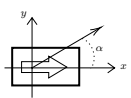
\includegraphics[width=0.2\linewidth]{immagini/5_image_0.png}
\end{center}

Immaginiamo adesso che il fascio luminoso sia polarizzato linearmente lungo una direzione che forma un angolo $\alpha$ con l'asse $x$. In MC trascurando la fase oscillante $(kz - \omega t)$ che non gioca alcun ruolo in quello che vogliamo discutere, possiamo semplicemente decomporre l'ampiezza del campo elettrico incidente in

$$E_{i n}=E_{0}\cos\alpha x+E_{0}\sin\alpha y$$

Subito dopo il filtro polarizzatore l'ampiezza risulta essere

$$E_{o u t}=E_{0}\cos\alpha x$$

Poich\'e l'intensit\'a \'e proporzionale al quadrato del campo elettrico, la frazione di energia del fascio che attraversa il polarizzatore nell'unit\'a di tempo arbitrario \'e dato dalla legge di Malus

$$T={\frac{I_{o u t}}{I_{i n}}}=\cos^{2}\alpha x$$

in cui la luce trasmessa ha la stessa frequenza della luce incidente. Reinterpretiamo il risultato in termini di fotoni identici. Per semplificare la trattazione possiamo immaginare che l'intensit\'a del fascio incidente sia cos\'i debole che i fotoni arrivino sul polarizzatore (e sul rivelatore posto dopo il polarizzatore) uno alla volta. Il singolo fotone pu'o o attraversare o non attraversare il polarizzatore e nel primo caso verr\'a rivelato (una frazione pari a $\cos^2 \alpha x$), nel secondo no (una frazione pari a $1 - \cos^2 \alpha x$). Com\'e possibile che fotoni identici si comportino diversamente? La risposta della MQ \'e che il determinismo viene meno: \'e impossibile prevedere se un singolo fotone venga assorbito o trasmesso, il meglio che possiamo fare \'e prevedere le probabilit\'a che questo accada. Lo scettico potrebbe rispondere che esistono delle variabili nascoste, che sfuggono alle nostre misure sperimentali, che differenziano i fotoni che passano da quelli che non passano. Tuttavia \'e stato dimostrato dal teorico John Bell ed altri, come sia possibile distinguere sperimentalmente tra la MQ e le teorie con variabili nascoste. Ingegnosi esperimenti hanno consentito di falsificare la maggior parte delle teorie con variabili nascoste.
\end{enumerate}

\newpage

\vspace{5em}
\section{\huge Formalismo della MQ ad un determinato istante di tempo}

L'obiettivo di questo capitolo \'e introdurre un formalismo generale che possa essere applicato a una vasta classe di sistemi per la descrizione degli stati e delle grandezze fisiche osservabili delle quali vogliamo saper calcolare i risultati della misura, la probabilit\'a che una loro misura fornisca un determinato valore e, a partire da questo, il valore medio in uno stato e la fluttuazione attorno un valore arbitrario. Tutto questo deve essere fatto in accordo con le caratteristiche fondamentali della MQ: l'interpretazione probabilistica, le relazioni di indeterminazione e la quantizzazione di certe grandezze fisiche.

Iniziamo imponendo alcune restrizioni semplificartici:
\begin{enumerate}
\item Consideriamo sistemi con un numero finito N di gradi di libert\'a 

\item Daremo una trattazione non relativistica della MQ, che ci permetter\'a di considerare in modo diverso lo spazio-tempo, non pi'u come semplici coordinate, ma come operatori. Questi limiti saranno superati poi con la teoria relativistica dei campi.

\item adotteremo un formalismo hamiltoniano per la descrizione del sistema fisico
\end{enumerate}

\subsection{Descrizione degli stati}

Conoscere lo stato di un sistema fisico significa avere a disposizione l'informazione massima che possiamo acquisire su tale sistema effettuando operazioni che siamo fisicamente in grado di eseguire su di esso (\textit{stato puro}), ma anche un'informazione parziale se per qualche motivo quella massima ci 'e preclusa (\textit{stati misti}), a cui poi dovremmo applicare i concetti della fisica statistica.


\subsubsection{Stati in MC}

In MC la descrizione dello stato di un sistema 'e completamente determinata nel momento in cui abbiamo a disposizione i valori delle coordinate generalizzate e dei loro momenti coniugati, misurati ad un tempo iniziale $t_0$:

$$[q_i(t_0), p_i(t_0)]_{i=1, \ldots, N}$$

Sappiamo dal formalismo hamiltoniano classico che, note queste condizioni iniziali, lo stato del sistema a qualsiasi istante successivo $t > t_0$ \'e completamente determinato attraverso le equazioni del moto

\begin{equation}
	{\dot{q}}_{i}={\frac{\partial H}{\partial p_{i}}}\qquad\qquad{\dot{p}}_{i}=-{\frac{\partial H}{\partial q_{i}}}
\end{equation}

Conoscendo con precisione arbitraria le condizioni iniziali, possiamo conoscere ugualmente con precisione arbitraria anche le $[q_i(t), p_i(t)]$ per istanti successivi e le funzioni $f(q, p)$ di queste due osservabili, grazie all'introduzione delle parentesi di Poisson:

$${\frac{\mathrm{d}f}{\mathrm{d}t}}=\sum_{i=1}^{N}{\frac{\partial f}{\partial q_{i}}}{\frac{\mathrm{d}q_{i}}{\mathrm{d}t}}+{\frac{\partial f}{\partial p_{i}}}{\frac{\mathrm{d}p_{i}}{\mathrm{d}t}}=\sum_{i=1}^{N}{\frac{\partial f}{\partial q_{i}}}{\frac{\partial H}{\partial p_{i}}}-{\frac{\partial f}{\partial p_{i}}}{\frac{\partial H}{\partial q_{i}}}=\{f,H\}$$


\subsubsection{Stati In MQ}

Dal punto di vista quantistico questa trattazione non \'e accettabile perch\'e viola il principio di indeterminazione, che non ci consente di conoscere simultaneamente i valori delle variabili tra loro coniugate con precisione arbitraria, ma anche perch\'e dobbiamo considerare l'aspetto probabilistico della MQ.

Per capire come generalizzare la descrizione dell'evoluzione dello stato in MQ consideriamo un sistema molto semplice di una singola particella priva di spin, che si muove in una dimensione spaziale infinita $x$. Lo stato di questa particella \'e descritto dalla funzione d'onda $\Psi(x)$, che ovviamente non potr\'a essere una funzione qualsiasi, ma dovr\'a rispettare alcune regole fondamentali per poter essere associata alla particella. Dal contributo di Born, sappiamo che $\Psi(x)$ \'e legata alla densit\'a di probabilit\'a $P(x)$ di trovare la particella in un intorno della posizione $x$, per cui dovr\'a necessariamente essere:

\begin{equation}
	P(x)\geq0 \qquad \int{\rm d}x\,P(x)=1\qquad P(x)=\frac{|\Psi(x)|^{2}}{\parallel\Psi(x)\parallel^{2}}
\end{equation}

Da questa definizione ricaviamo due condizioni a cui deve sottostare la funzione d'onda: innanzitutto non pu\'o essere una funzione identicamente nulla, matematicamente perch\'e avrebbe norma nulla e quindi la frazione divergerebbe, fisicamente perch\'e non descriverebbe alcuno stato, in secondo luogo dovr\'a appartenerne a quel gruppo di funzioni modulo quadro integrabili per poter rispettare la condizione imposta dalla probabilit\'a, chiamiamo questo gruppo $L_2(\mathbb{R})$

\begin{equation}
	\left\|\Psi\right\|^{2}=\int{\rm d}x\left|\Psi\right|^{2}<\infty\quad\text{e} \quad\Psi(-\infty)=\Psi(+\infty)=0\quad\longrightarrow\quad\Psi(x)\in L_{2}(\mathbb{R})
\end{equation}

Osserviamo che se $\Psi(x)$ descrive lo stato di un sistema, anche $\alpha\Psi(x)$ con $\alpha \in \mathbb{C} - {0}$ descrive lo stesso stato, perch\'e nel calcolo della densit\'a di probabilit\'a la costante moltiplicativa si elide e otteniamo lo stesso risultato.


\textbf{Richiami sugli spazi di Hilbert}

Dato che $L_2(\mathbb{R})$ \'e uno \textit{spazio di Hilbert}, richiamiamo alcuni concetti fondamentali su questi spazi. $\mathcal{H}$ \'e uno \textit{spazio vettoriale complesso}, i cui vettori si indicano con il simbolo di \textit{ket} $|\Psi\rangle$; questo significa che presi due vettori in esso, anche la loro combinazione lineare appartiene a $\mathcal{H}$

$$\alpha,\beta\in\mathbb{C}\quad \text{e}\quad(|\Psi\rangle\,,|\Phi\rangle)\in\mathcal{H}\quad\longrightarrow\quad(\alpha\,|\Psi\rangle+\beta\,|\Phi\rangle\,)\in\mathcal{H}\,$$
ci'o 'e necessario per la linearit\'a della MQ che fa valere il principio di sovrapposizione. Poi, 'e presente un *prodotto* scalare definito positivo, cio'e possiamo associare a due vettori uno specifico numero complesso

$$(\left|\Psi\right\rangle,\left|\Phi\right\rangle)\in{\mathcal{H}}\quad\longrightarrow\quad\left\langle\Psi|\Phi\right\rangle\in{\mathbb{C}}$$

che gode delle ben note propriet\'a:

$$\langle\Psi|\Phi\rangle=\langle\Phi|\Psi\rangle^{*}$$
$$\braket{\Phi}{\lambda_{1}\Psi_1 + \lambda_{2}\Psi_2} = \lambda_{1}\braket{\Phi}{\Psi_{1}} + \lambda_{2}\braket{\Phi}{\Psi_{2}} \qquad\qquad 
\braket{\lambda_{1}\Psi_{1} + \lambda_{2}\Psi_{2}}{\Phi} = \lambda_{1}^* \braket{\Psi_{1}}{\Phi} + \lambda_{2}^* \braket{\Psi_{2}}{\Phi}$$
$$||\Psi||2 = \braket{\Psi}{\Psi} \geq 0 \qquad\qquad = 0 \iff \ket{\Psi} = 0$$

Inoltre $\mathcal{H}$ \'e \textit{completo}, cio\'e ogni successione di Cauchy $\{\ket{\Psi_n}\}$ converge in $\mathcal{H}$:

$$\operatorname*{lim}_{m,n\to\infty}||\Psi_{m}-\Psi_{n}||=0\quad\exists\,|\Psi\rangle\in{\mathcal{H}}\quad\left|\quad\operatorname*{lim}_{n\to\infty}||\Psi-\Psi_{n}||=0\right.$$

Infine \'e \textit{separabile}, quindi esistite una base numerabile e densa ovunque per i vettori di $\mathcal{H}$, e non \'e restrittivo prenderla ortonormale $\{\ket{u_n}\}$. Questo ci consente di scrivere ogni vettore dello spazio di Hilbert come combinazione lineare dei vettori di base

$$|\Psi\rangle=\sum_{n}c_{n}\,|u_{n}\rangle\qquad\langle u_{n}|u_{m}\rangle=\delta_{m n}$$

e moltiplicando a destra per il \textit{bra} $\bra{u_n}$ (un \textit{bra} altro non \'e che il complesso coniugato di un vettore) otteniamo la relazione

$$\langle u_{n}|\Psi\rangle=c_{n}\quad\longrightarrow\quad|\Psi\rangle=\sum_{n}|u_{n}\rangle\,\langle u_{n}|\Psi\rangle$$

Ci\'o che abbiamo fatto ha un importante risvolto pratico che scopriremo proseguendo nello studio della MQ,
infatti la quantit\'a $\sum_n \ket{u_n}\bra{u_n}$ rappresenta l'operatore identit\'a e si chiama \textit{relazione di completezza} dello spazio hilbertiano, si usa spessissimo nell'ambito degli operatori.

Notiamo che se prendiamo un'arbitraria combinazione lineare dei vettori di base dello spazio di Hilbert, infinita e numerabile, non \'e detto che il vettore corrispondente sia in $L_2$, perch\'e \'e necessario verificare che abbia norma finita, cio\'e che i suoi coefficienti soddisfino

$$\langle\Psi|\Psi\rangle=\sum_{n}|c_{n}|^{2}<\infty$$

Tutta l'informazione fornita da $\Psi(x)$ \'e reperibile anche dalla sua trasformata di Fourier, 

${\tilde{\Psi}}(p)=\left[L_{2}(\mathbb{R})\right]_{p}$

$$\tilde{\Psi}(p) = \frac{1}{\sqrt{2\pi\hbar}} \int \mathrm{d}x \Psi(x) e^{-i\frac{px}{\hbar}} \qquad\qquad \text{con} \Psi(x) = \frac{1}{\sqrt{2\pi\hbar}} \int \mathrm{d}p \tilde{\Psi} e^{i\frac{px}{\hbar}} \text{ antitrasformata}$$

il cui spazio di appartenenza \'e isomorfo $L_2(\mathbb{R})$. La presenza di $\hbar$ come fattore di normalizzazione e come fattore dell'esponenziale \'e dovuto al fatto che nella definizione rigorosa \'e presente il vettore d'onda $k$, legato al momento dalla relazione $k = \frac{p}{\hbar}$. La trasformata \'e una funzione definita nello spazio delle $p$ da cui \'e possibile ricavare la densit\'a di probabilit\'a di trovare una particella in un intorno di un determinato valore dell'impulso, in modo analogo a quanto fatto per la funzione nello spazio delle coordinate

$$P(p)=\frac{|\tilde{\Psi}(p)|^{2}}{||\tilde{\Psi}(p)||^{2}}$$

Tra trasformata e antitrasformata vale l'\textit{identit\'a di Parseval}, per la quale descrivere il sistema in un modo o nell'altro \'e del tutto equivalente 

$$||\Psi||^2 = ||\tilde{\Psi}||^2$$

Quanto appena detto deriva dal fatto che possiamo dimostrare che tutti gli spazi di Hilbert che hanno la stessa cardinalit\'a sono isomorfi tra loro; questo fatto ci suggerisce di sviluppare un formalismo in cui lo stato del sistema non sia legato alla particolare scelta della variabile da cui dipende la funzione d'onda, ma che ci sia un \textit{vettore astratto} di uno spazio di Hilbert, poi se risulta necessario potremo specificare una \textit{rappresentazione concreta}.

Detto questo, enunciamo il primo postulato della MQ:

\textbf{\textit{Postulato 1. Degli stati}} 

\textit{Ogni sistema quantistico $\mathcal{S}$ pu\'o essere associato ad uno spazio di Hilbert astratto $\mathcal{H}$, e ogni stato (puro) $\Sigma$ del sistema pu\'o essere associato a un raggio vettore complesso $\hat{\Psi} \in \mathcal{H}$.}

Introduciamo quindi la nozione importante di \textit{raggio vettore}, che \'e definito come la classe di equivalenza dei vettori che puntano nella stessa direzione

$${\hat{\Psi}}=\{\lambda\,|\Psi\rangle\quad\big|\quad\lambda\in\mathbb{C}-0\}$$

infatti come abbiamo detto in precedenza, tutti i $\lambda \ket{Psi}$ rappresentano lo stesso stato. Per rappresentare un raggio vettore possiamo scegliere un qualsiasi elemento rappresentativo della classe, solamente per comodit\'a lo prendiamo normalizzato, nel caso non lo fosse non dobbiamo dimenticare il fattore di normalizzazione necessario nella definizione di probabilit\'a.

Notiamo alcune cose: la prima \'e che la presenza della costante $\lambda$ include la possibilit\'a di avere una fase arbitraria pur essendo presente la normalizzazione, la seconda \'e che nel postulato valgono le implicazioni opposte, cio\'e a uno spazio di Hilbert \'e associabile un sistema quantistico e ad una raggio vettore uno stato puro, tranne in alcuni casi particolari che non tratteremo.


\textbf{Rappresentazioni $x$ e $p$}

Quando in MC abbiamo parlato di onde, abbiamo detto che quelle piane monocromatiche, che sono infinitamente estese, non sono realizzabili fisicamente ma le abbiamo comunque sfruttate per determinare la struttura matematica dei pacchetti, che invece hanno estensione ed energia finite, mediante integrale di Fourier.

Ora siamo di fronte allo stesso tipo di problema e la soluzione finale avr\'a la stessa struttura logica: abbiamo scritto $\Psi(x)$ come l'integrale di Fourier di esponenziali pesati da opportuni coefficienti dati dalla trasformata:

$$u_{p}(x)={\frac{1}{\sqrt{2\pi\hbar}}}e^{i{\frac{p x}{\hbar}}}\ \ \ \ \notin L_{2}(\mathbb{R})$$

Notiamo subito che questo tipo di funzioni non sono modulo quadro integrabili, tuttavia ci\'o non ci impedisce di interpretare questo insieme di oggetti come una \textit{base ortonormale generalizzata nel senso delle distribuzioni}, per le quali vale la relazione di ortonormalit\'a generalizzata (con la $\delta$ di Dirac) e di completezza

$$u_{p}u_{p}^{\prime}=\int\mathrm{d}x\,u_{p}^{*}(x)u_{p^{\prime}}(x)=\frac{1}{2\pi}\int\frac{d x}{\hbar}e^{-i\,\frac{x}{\hbar}(p-p^{\prime})}=\delta(p-p^{\prime})$$

$$\int\mathrm{d}x\,u_{p}^{*}(x^{\prime})u_{p}(x)=\frac{1}{2\pi}\int\frac{d x}{\hbar}e^{-i\frac{p}{\hbar}(x-x^{\prime})}d x=\delta(x-x^{\prime})$$

Allo stesso modo possiamo introdurre una base generalizzata con indici continui legati alla posizione della particella: $\xi_{x_0} (x) = \delta(x - x_0) \notin L_2(\mathbb{R})$

$$(\xi_{x_{0}},\xi_{x_{0}^{\prime}})=\int\mathrm{d}x\,\delta(x-x_{0})\delta(x-x_{0}^{\prime})=\delta(x_{0}-x_{0}^{\prime})$$
$$\int\mathrm{d}x_{0}\,\xi_{x_{0}}^{*}(x^{\prime})\xi_{x_{0}}(x)=\int\mathrm{d}x_{0}\,\delta(x_{0}-x^{\prime})\delta(x_{0}-x)=\delta(x-x^{\prime})$$  

A queste basi possiamo associare i \textit{ket} generalizzati $|x_{0}\rangle\,,|p_{0}\rangle$ e scrivere le relazioni di completezza generalizzate 

$$\begin{matrix}\langle x_0|x'_0\rangle=\delta(x_0-x'_0)&\int\mathrm{d}x_0\,|x_0\rangle\langle x_0|=1\\ \langle p_0|p_0\rangle=\delta(p_0-p_0')&\int\mathrm{d}p_0\,|p_0\rangle\langle p_0|=1\end{matrix}$$ 

grazie alle qual possiamo scrivere la funzione d'onda in modo estremamente intuitivo ed efficace
 
$$\langle x|\Psi\rangle=\langle x|\mathbbm{1}|\Psi\rangle=\int\mathrm{d}x\,\langle x|x_{0}\rangle\,\langle x_{0}|\Psi\rangle=\delta(x-x_{0})\int\mathrm{d}x^{\prime}\,\xi_{x_{0}}^{*}(x^{\prime})\Psi(x^{\prime})=\int\mathrm{d}x^{\prime}\,\delta(x-x^{\prime})\Psi(x^{\prime})=\Psi(x)\,.$$
$$\langle p|\Psi\rangle=\ldots={\tilde{\Psi}}(p)$$

\subsection{Descrizione delle osservabili}

Le osservabili sono tutte quelle quantit\'a che possiamo misurare con operazioni fisicamente eseguibili sul sistema, come per esempio l'energia, la velocit\'a, la posizione, ecc. Tutto ci\'o che possiamo sperare di misurare in laboratorio sulle osservabili \'e il valore medio in un dato stato.

\subsubsection{Spettro di un'osservabile}

In generale dobbiamo distinguere tra l'osservabile fisica e l'operatore matematico che la descrive, quindi chiamiamo A la prima e A il secondo. Possiamo per\'o identificare i due oggetti in base al postulato 3 che enunceremo in seguito, quindi la maggior parte delle volte verr\'a meno la distinzione tra i due.

Misurando questa osservabile, otteniamo certi valori che racchiudiamo in un insieme chiamato \textit{spettro}:

\textbf{Definizione 1.} \textit{Lo spettro di un'osservabile, che scriviamo come $\sigma(\mathcal{A})$, \'e l'insieme dei valori che possiamo ottenere con una misura di $\mathcal{A}$ prendendo in considerazione tutti i possibili stati del sistema}.

Ovviamente si deve verificare che $\sigma \mathcal{A} \subseteq \mathbb{R}$ dato che stiamo parlando di misure fisicamente eseguibili (di certo non potremmo trovare un valore complesso). Lo spettro di un'osservabile pu\'o essere sia \textit{puramente discreto} (come per esempio quello per una particella senza spin in una buca di potenziale infinita), oppure \textit{puramente continuo} (per una particella libera); in alcune occasioni pu\'o presentarsi uno \textit{spettro misto} dato dalla somma di una parte discreta e di una continua (\'e il caso della particella in una buca di potenziale di profondit\'a finita),
quindi in generale scriviamo 

$$\sigma(\mathcal{A}) = \sigma_d(\mathcal{A}) + \sigma_{c}(\mathcal{A})$$

Vediamo ora cosa possiamo dire sul valore medio dell'osservabile $\mathcal{A}$ nello stato $\Sigma$. Diamone una definizione matematica operativa 

\textbf{Definizione 2.} \textit{Consideriamo un numero $N$ molto grande di copie del sistema nello stesso stato}\footnote{Questo concetto \'e piuttosto sottile, non \'e totalmente corretto dire che si effettuano $N$ misure sullo stesso sistema nello stesso stato, questo perch\'e lo studio degli effetti della misura in MQ \'e una questione delicata e tutt'ora non risolta}
\textit{, ed effettuiamo $N$ misure dell'osservabile $\mathcal{A}$ che forniscono un certo risultato, allora il valore medio di $\mathcal{A}$ \'e:}

$$\langle A\rangle_{\Sigma}\equiv\operatorname*{lim}_{N\rightarrow\infty}{\frac{a_{1}+...+a_{N}}{N}}$$

\textit{Accanto al valore medio possiamo considerare anche la fluttuazione quadratica media attorno un certo numero arbitrario reale, definita come}

$$(\Delta\mathcal{A})_{a} \equiv \sqrt{\langle (\mathcal{A} - a)^2 \rangle}$$



\subsubsection{Osservabili in MC}

Nella MC, sappiamo che lo stato fisico iniziale del sistema \'e descritto matematicamente dalle coordinate generalizzate e dagli impulsi generalizzati $(q_0, p_0)$ ad un certo istante $t_0$; poi da questo punto nello spazio delle fasi possiamo ricavare lo stato a qualsiasi istante di tempo successivo tramite le equazioni della meccanica hamiltoniana; questo vale anche per qualsiasi funzione di $(q, p)$, che sappiamo rappresentare un'osservabile: una misura di A dar\'a sempre lo stesso risultato perch\'e non \'e contemplata alcuna fluttuazione dei valori misurati.

Quindi possiamo dire che \textit{lo spettro di un'osservabile in MC \'e semplicemente il codominio della funzione che la descrive, cio\'e i valori che questa funzione pu\'o assumere quando facciamo variare le coordinate nel loro intervallo di validit\'a}.


\subsubsection{Osservabili in MQ}

In MQ la trattazione assume un aspetto pi\'u complicato perch\'e non possiamo trascurare l'interpretazione probabilistica e le relazioni di indeterminazione che ci impediscono di conoscere con precisione arbitraria variabili tra loro coniugate, per non parlare poi della quantizzazione di certe osservabili.

Iniziamo la trattazione sullo spettro vedendo un esempio semplice. Consideriamo una particella priva di spin che si muove lungo la direzione $x$. Il suo stato \'e descritto dalla funzione $\Psi(x) \in L_2(\mathbb{R})$ e le osservabili fondamentali sono la posizione $X$ e la corrispondente componente dell'impulso $P_X$, a cui sappiamo sono associati degli operatori che agiscono su una funzione come:

\begin{equation}
	X\left|\Psi\right\rangle=x\left|\Psi\right\rangle\longrightarrow X\Psi(x)=x\Psi(x)\qquad\qquad P\left|\Psi\right\rangle=p\left|\Psi\right\rangle\longrightarrow P_{x}\Psi(x)=-i\hbar\frac{\mathrm{d}\Psi(x)}{\mathrm{d}x}
\end{equation}

A partire da questi due operatori possiamo esprimere qualsiasi altra grandezza mediante delle opportune funzioni, per esempio l'hamiltoniano (indipendente dal tempo)

\begin{equation}
	H={\frac{P^{2}}{2m}}+V(X)
\end{equation}

che rappresenta l'energia totale della particella nella sua componente cinetica e potenziale.


\textbf{Postulato 2. \textit{Delle osservabili}} 

\textit{Ad ogni osservabile $\mathcal{A}$ del sistema quantistico sar\'a associato un operatore lineare e autoaggiunto che chiamiamo $A \in \mathcal{H}$. Il valor medio di questa osservabile nello stato $\Sigma$ \'e dato partendo da un qualsiasi vettore $\Psi$ nello spazio di Hilbert che rappresenta lo stato}

$$\langle A\rangle_{\Sigma}=\frac{\langle\Psi|A|\Psi\rangle}{\langle\Psi|\Psi\rangle}$$

Dopo aver ricordato che un operatore 'e autoaggiunto se 'e uguale al suo aggiunto, cio'e se si verifica che

$$\forall\left|\Psi\right\rangle,\left|\Phi\right\rangle\in\mathcal{D}(A) \qquad\qquad \left\langle\Psi|A\Phi\right\rangle=\left\langle A\Psi|\Phi\right\rangle \qquad\qquad \text{ con } {\mathcal{D}}(A)={\mathcal{D}}(A^{+})$$

elenchiamo alcune caratteristiche che devono avere gli operatori associati alle osservabili secondo questo postulato le seguenti:
\begin{enumerate}
	\item $A$ deve essere un operatore lineare perch\'e vogliamo che valga il principio di sovrapposizione
	
	$$A(\lambda_{1}\Psi_{1}+\lambda_{2}\Psi_{2})=\lambda_{1}A\Psi_{1}+\lambda_{2}A\Psi_{2}$$
	
	Questo fatto \'e importante perch\'e il valore medio dell'osservabile rimanga lo stesso anche se moltiplichiamo il vettore di stato per una costante diversa da zero.
	
	\item Il dominio $\mathcal{D}(A)$ di $A$ deve essere denso in $\mathcal{H}$. Questa richiesta \'e necessaria perch\'e non tutti gli operatori sono definiti su tutto lo spazio di Hilbert: per spazi di Hilbert di dimensione finita non ci sono problemi perch\'e il dominio dell'operatore \'e tutto $\mathcal{H}$, ma per operatori illimitati in spazi di Hilbert di dimensione infinita questo non \'e automatico. Dobbiamo chiedere qualcosa in meno della relazione $\mathcal{D}(A) = \mathcal{H}$, cio\'e dobbiamo chiedere almeno che $\mathcal{D}(A)$ sia denso in $\mathcal{H}$, questo ci permette di "approssimare bene quanto vogliamo" un qualsiasi vettore nello spazio di Hilbert, che potr\'a essere scritto come limite di una successione di stati che appartengono a $\mathcal{D}(A)$
	
	$$\forall\Psi\in\mathcal{H},\exists\{\Psi_{n}\}\subset\mathcal{D}(A)\quad\left|\quad\lim_{n\to\infty}||\Psi_{n}-\Psi||=0\quad\longrightarrow\quad\langle\mathcal{A}\rangle=\lim_{n\to\infty}\frac{\langle\Psi|A|\Psi_{n}\rangle}{\langle\Psi|\Psi\rangle}\right|$$
	
	\item $A$ \'e hermitiano, cio\'e per ogni coppia di vettori $\ket{\Psi}, \ket{\Phi} \in \mathcal{D}(A)$ vale
	
	$$\braket{\phi}{A\Psi} = \braket{A\Psi}{\Phi}$$
	
	\'E importante che questa condizione venga rispettata perch\'e \'e quella necessaria e sufficiente perch\'e i valori medi siano reali, e come sappiamo ci\'o \'e fondamentale per un operatore che ha la pretesa di descrivere osservabili fisiche. Dimostriamo che un operatore \'e hermitiano se e solo se ha valori medi reali.
	
	
	\textit{Dimostrazione}. Consideriamo il caso semplificato $\ket{\Psi} = \ket{\Phi}$ che non fa perdere di generalit\'a, e dimostriamo che $\bra{\Psi|A}\ket{\Psi} \in \mathbb{R}$
	\begin{equation*}
		\begin{array}{l l}
			\braket{\Psi}{A\Psi} = \braket{A\Psi}{\Psi}^* & \text{ prop. prodotto scalare}
			\\
			\braket{\Psi}{A\Psi} = \braket{A\Psi}{\Psi} & \text{ definizione di hermitiano}
		\end{array}
		\longrightarrow \braket{A\Psi}{\Psi}^* = \braket{A\Psi}{\Psi} \text{ definizione di valore medio reale}
	\end{equation*}
	
	Mostriamo ora il viceversa, cio\'e che a valori medi reali corrispondono operatori hermitiani. Consideriamo uno stato $\ket{\Psi}$ e scriviamolo come combinazione di altri due stati di cui uno moltiplicato per un fattore di fase non banale
	
	$$|\Psi\rangle=|f\rangle+e^{i\alpha}\,|g\rangle\qquad|f\rangle\,,|g\rangle\in{\mathcal{D}}(A)$$
	
	allora
	
	$$\langle\Psi|A\Psi\rangle=\big{(}\,\langle f|+e^{-i\alpha}\,\langle g|\,\big{)}A\big{(}\,|f\rangle+e^{i\alpha}\,|g\rangle\,\big{)}=\langle f|A|f\rangle+\,\langle g|A|g\rangle+e^{i\alpha}\,\langle f|Ag\rangle+e^{-i\alpha}\,\langle g|Af\rangle$$
	
	scegliendo prima $\alpha = 0$ e poi $\alpha = \frac{\pi}{2}$ e dividendo questo secondo risultato per $i$ otteniamo le seguenti due equazioni
	
	$$\langle f|A g\rangle+\langle g|A f\rangle=\langle A f|g\rangle+\langle A g|f\rangle \qquad\qquad \langle f|A g\rangle-\langle g|A f\rangle=\langle A f|g\rangle-\langle A g|f\rangle$$
	
	in cui abbiamo usato la definizione di valor medio reale; sommandole membro a membro otteniamo
	
	$$\langle f|A g\rangle=\langle A f|g\rangle\qquad\forall\left|f\right\rangle,\left|g\right\rangle\in{\mathcal{D}}(A)$$
	
	che \'e la condizione di hermiticit\'a per un operatore. $\qquad\square$
\end{enumerate}

Passiamo ora a dare la rappresentazione matriciale di un operatore. Data la base ortonormale $\{|\ket{u_n}\}$, possiamo scrivere il vettore $\Psi_n$ grazie alla rappresentazione \textit{bra-ket}: $\Psi_n = \braket{u_n}{\Psi}$. Da ci\'o deduciamo che il generico vettore $\ket{\Psi}$ \'e dato dalla somma delle proiezioni lungo i vettori di base mediante la relazione di completezza di cui avevamo parlato in precedenza

$$|\Psi\rangle=\sum_{n}|\mu_{n}\rangle\,\langle\mu_{n}|\Psi\rangle$$

Consideriamo anche un operatore $O$ che agisce su $\Psi$ come $O\left|\Psi\right\rangle=\left|\Psi^{\prime}\right\rangle$, allora

$$\Psi_{m}^{\prime}=\langle\mu_{m}|\Psi^{\prime}\rangle=\langle\mu_{m}|O|\Psi\rangle=\sum_{n}\,\langle\mu_{m}|O|\mu_{n}\rangle\,\Psi_{m}=\sum_{m n}O_{m n}\Psi_{n}\,,$$

In via pi\'u in generale, avendo a disposizione anche un altro vettore $\ket{\Phi}$, vale:

$$|\Psi\rangle=\sum_{m}\Psi_{m}\,|\mu_{m}\rangle\quad|\Phi\rangle=\sum_{n}\Phi_{n}\,|\mu_{n}\rangle\quad\longrightarrow\quad\langle\Psi|O|\Phi\rangle=\sum_{m n}\Psi_{m}^{*}O_{m n}\Phi_{n}=\Psi^{*}O\Phi\,.$$

Il termine $O_{mn}$ \'e chiamato \textit{elemento di matrice dell'osservabile $O$ fra $\ket{\Psi}$ e $\ket{\Phi}$}, infatti formalmente un operatore \'e ben rappresentato da una matrice i cui elementi sono proprio questi termini, che in questo caso sono posizionati nella $m$-esima riga e $n$-esima colonna.

\textbf{Postulato 3. \textit{Possibili risultati delle misure}} 

\textit{Gli unici risultati possibili per una misura dell'osservabile $A$ sono tutti e soli gli autovalori dell'operatore $A$, quindi vale}

$$\sigma({\mathcal{A}})=\sigma(A)$$

Questo postulato in realt\'a si potrebbe dimostrare, facendo vedere come $\sigma(\mathcal{A}) \subseteq \sigma(A)$ e poi $\sigma(\mathcal{A}) \supseteq \sigma(A)$, che porta inevitabilmente all'uguaglianza. Nel caso discreto lo spettro \'e definito come l'insieme degli autovalori che soddisfano l'equazione agli autovalori per l'operatore che descrive l'osservabile:

$$\sigma_{d}(A)=\{a\in\mathbb{R},\quad\exists\,|\Psi_{\alpha}\rangle\in\mathcal{D}(A)\quad\left|\quad A\,|\Psi_{\alpha}\rangle=a\,|\Psi_{\alpha}\rangle\right\}$$

e in questo contesto possiamo anche dimostrare che gli autovalori di un operatore hermitiano relativi ad autovalori distinti $a_n \neq a_m (\forall m \neq n)$ sono ortogonali; infatti se vale $A \ket{a_m} = a_m\ket{a_m}$ e $A \ket{a_n} = a_n \ket{a_n}$, allora

$$\left(a_{m}-a_{n}\right)\left\langle a_{m}|a_{n}\right\rangle=\left\langle Aa_{m}|a_{n}\right\rangle-\left\langle a_{m}|Aa_{n}\right\rangle=\left\langle Aa_{m}|a_{n}\right\rangle-\left\langle Aa_{m}|a_{n}\right\rangle=0\quad\Longleftrightarrow\quad\left\langle a_{m}|a_{n}\right\rangle=0$$

per definizione di $A$ hermitiano.

Diremo che $A$ \'e \textit{non degenere} se non esistono due autovettori relativi allo stesso autovalore linearmente indipendenti; invece diremo che \'e \textit{degenere con grado di degenerazione} $d$ quando esistono $d$ autovettori $ \{ \ket{\Psi_\alpha^i} \}_{i=1, \ldots, d} $ linearmente indipendenti relativi allo stesso autovalore, questi autovettori formano uno spazio di Hilbert $\mathcal{H}_d \subset \mathcal{H}$
di dimensione $d$. 


\textbf{Postulato 4. \textit{Probabilit\'a di ottenere un dato risultato da una misura}}

\textit{La probabilit\'a che una misura di $A$ nello stato $\ket{\Psi}$ dia come risultato $a_k \in \sigma_d(A)$, con $\braket{a_k}{a_k} = 1$ e $A \ket{a_k} = a_k \ket{a_k}$, \'e data da}

$$w(a_{k})={\frac{\mid\langle a_{k}|\Psi\rangle\mid^{2}}{\langle\Psi|\Psi\rangle}}$$

A seconda della tipologia di spettro che presenta l'osservabile, possiamo distinguere tre differenti casistiche per la base ortonormale, e di conseguenza tre scritture per tale probabilit\'a:
\begin{itemize}
	\item Se lo spettro 'e discreto e non degenere, possiamo costruire la base ortonormale di autovettori $\{\ket{a_k}\}$ e scrivere la funzione d'onda come una loro combinazione lineare, di conseguenza la probabilit\'a avr\'a una forma semplificata

	$$|\Psi\rangle=\sum_{n}c_{n}\,|a_{n}\rangle\quad\longrightarrow\quad w(a_{k})={\frac{|c_{k}|^{2}}{||\Psi||^{2}}}$$

	\item Invece se lo spettro 'e discreto ma degenere di grado $d$, la base necessita di un indice aggiuntivo che conta la degenerazione $\{ \ket{a_{k,i}}_{i=1,...,d}\}$, questo si ripercuote nella scrittura del vettore e della probabilit\'a

	$$|\Psi\rangle=\sum_{R}\sum_{i=1}^{d_{R}}c_{k,i}\,|a_{k,i}\rangle\quad\longrightarrow\quad w(a_{k})=\sum_{i=1}^{d_{R}}\frac{|\,\langle a_{k,i}|\Psi\rangle\,|^{2}}{||\Psi||^{2}}=\sum_{i=1}^{d_{R}}\frac{|c_{k,i}|^{2}}{||\Psi||^{2}}\,.$$

	\item Se siamo di fronte ad uno spettro continuo, la base generalizzata sar\'a $\{\ket{a}\}$ che rispetta le condizioni $\braket{a^\prime}{a} = \delta(a-a^\prime)$ e $c(a) = \braket{a}{\Psi}$, e il vettore si scriver\'a $\ket{\Psi} = \int c(a)\ket{a} \mathrm{d}a$. In questo caso ha senso domandarsi qual \'e la probabilit\'a di trovare $\mathcal{A}$ in un range (anche infinitesimo) $a \pm \mathrm{d}a$ attorno all'autovalore\footnote{Dato che lo strumento non sar\'a infinitamente preciso, non possiamo chiedere la probabilit\'a di trovare esattamente il valore $a$}, e possiamo anche ricavare la funzione densit\'a di probabilit\'a:

	$$\mathrm{d} w(a)=\rho(a)\mathrm{d} a={\frac{\mid\langle a|\Psi\rangle\mid^{2}}{||\Psi||^{2}}}\,\mathrm{d}a={\frac{|c(a)|^{2}}{||\Psi||^{2}}}\,\mathrm{d}a\quad\longrightarrow\quad\rho(a)={\frac{|c(a)|^{2}}{||\Psi||^{2}}}\,\mathrm{d}a$$
\end{itemize}

Proseguiamo lo studio delle osservabili enunciando un teorema di cui non diamo la dimostrazione:

\begin{theorem} \textbf{Teorema spettrale}
	Dato un operatore autoaggiunto $A$ associato ad una certa osservabile $\mathcal{A}$, ogni stato $\ket{\Psi}$ dello spazio di Hilbert si pu\'o decomporre in una base ortonormale costituita tutta da autovettori di questo operatore. Quindi nel caso di spettro discreto la base ortonormale sar\'a $\ket{a_{k,i}}$
	
	$$|\Psi\rangle=\sum_{k}\sum_{i=1}^{d_{k}}c_{k}^{i}\,|a_{k,i}\rangle$$
	
	e nel caso di spettro continuo ci sar\'a una relazione analoga generalizzata
	
	$$|\Psi\rangle=\int\mathrm{d}a\,c\,|a\rangle$$
	
	Questo risultato \'e importante perch\'e ci permette di arrivare facilmente a predizioni fisiche sia per i risultati delle misure, che per l'evoluzione temporale.	
\end{theorem}


\subsubsection{Relazioni di indeterminazione}

Ora abbiamo gli strumenti per dimostrare le relazioni di indeterminazione in modo generale, per poi calarci nel caso particolare di posizione-impulso del principio di indeterminazione di Heisenberg.

Consideriamo due operatori autoaggiunti $A, B$ e due numeri reali qualsiasi $a, b \in \mathbb{R}$, vogliamo dimostrare che il prodotto delle fluttuazioni quadratiche medie nello stato rappresentato dal vettore $\Psi$ soddisfa

$$(\Delta A)_{\Psi,a}(\Delta B)_{\Psi,b}\geq\frac{1}{2}\vert\left<[A,B]\right>_{\Psi}\vert$$

\textit{Dimostrazione}. Incominciamo definendo due nuovi operatori

$$\hat{A}=A-\,\mathbbm{1}a\qquad\hat{B}=B-\,\mathbbm{1}b$$

\'e evidente come anche questi siano autoaggiunti hermitiani, dato che $a$ e $b$ sono reali. Calcoliamo la fluttuazione quadratica media per l'operatore A, sapendo che poi varr\'a lo stesso per B

$$(\Delta A)^{2}_{\Psi,n}\equiv\frac{\langle\Psi|(A-a)^{2}|\Psi\rangle}{\langle\Psi|\Psi\rangle}=\frac{\langle\Psi|\hat{A}^{2}|\Psi\rangle}{||\Psi||^{2}}=\frac{\langle\hat{A}\Psi|\hat{A}\Psi\rangle}{||\Psi||^{2}}=\frac{||\hat{A}\Psi||^{2}}{||\Psi||^{2}}\qquad\qquad(\Delta B)^{2}_{\Psi,b}=\frac{||\hat{B}\Psi||^{2}}{||\Psi||^{2}}$$ 

$$\longrightarrow\quad(\Delta A)^{2}_{\Psi,a}(\Delta B)^{2}_{\Psi,b}=\frac{||\hat{A}\Psi||^{2}}{||\Psi||^{2}}\frac{||\hat{B}\Psi||^{2}}{||\Psi||^{2}}$$  

Introduciamo per semplicit\'a altri due operatori e dimostriamo che sono hermitiani

$$C=-i[A,B]=-i[\hat{A},\hat{B}]\qquad\qquad\{\hat{A},\hat{B}\}=\hat{A}\hat{B}+\hat{B}\hat{A}\quad\text{(anticommutatore)}.$$
	
	
$$C^+=\big(\,-\,i[A,B]\big)^+=+i(AB-BA)^+=+i(B^+A^+-A^+B^+)=+i(BA-AB)=\big(\,-\,i[A,B]\big)=C$$

$$\{\hat{A},\hat{B}\}^+=\big(\hat{A}\hat{B}+\hat{B}\hat{A}\big)^+=\hat{B}^+\hat{A}^++\hat{A}^+\hat{B}^+=\{\hat{A},\hat{B}\}$$

Giungiamo alla dimostrazione che ci eravamo prefissati di dare




\begin{align*}
	\parallel\hat{A}\Psi\parallel^2 \; \parallel\hat{B}\Psi\parallel^2  
	&\overbracket[0pt][0pt]{\geq}^{(a)}
	\big| \braket[\big]{\hat{A}\Psi}{\hat{B}\Psi} \big|^2 \overbracket[0pt][0pt]{=}^{(b)} \big| \braket[\big]{\Psi}{\hat{A}\hat{B}\Psi} \big|^2 
	\overbracket[0pt][0pt]{=}^{(c)} \bigg| \bra[\bigg]{\Psi} \frac{\{A, B\}}{2} \ket[\bigg]{\Psi} + \frac{i}{2} \bra{\Psi} C \ket{\Psi} \bigg|^2 =
	\\
	&\overbracket[0pt][0pt]{\geq}^{(d)} \frac{1}{4} \big( | \bra{\Psi}{A, B}\ket{\Psi} |^2 + \bra{\Psi} C \ket{\Psi} |^2 \big) \overbracket[0pt][0pt]{\geq}^{(e)} \frac{1}{4} | \bra{\Psi} C \ket{\Psi} |^2 
	\\
	&= \frac{1}{4} | \bra{\Psi} [A, B] \ket{\Psi} |^2 
	\\
	(\Delta A \Delta B)_\Psi 
	&\geq \frac{1}{2} \frac{\bra{\Psi} [A, B] \ket{\Psi}} {||\Psi||^2} = \frac{ 1}{ 2 } | \langle [A, B] \rangle_\Psi |
\end{align*}

in cui nel passaggio (a) abbiamo usato la disuguaglianza di Schwartz, in (b) la propriet\'a di autoaggiuntezza, in	(c) abbiamo riscritto il prodotto dei due operatori come somma del loro commutatore e anticommutatore, in (d) abbiamo sfruttato il fatto che il quadrato della somma di due numeri di cui uno reale e l'altro puramente immaginario \'e dato dalla somma dei quadrati perch\'e sono ortogonali nel piano complesso, infine in (e) abbiamo minorato semplicemente togliendo opportunamente uno dei due addendi. $\square$
	
Nel caso particolare in cui consideriamo gli operatori posizione e momento dobbiamo fare le sostituzioni $A \to X$ e $B \to P_X$, inoltre sappiamo gi\'a che $[X, P] = i\hbar$, quindi si ricava facilmente che
	
$$(\Delta X\Delta P)\geq{\frac{\hbar}{2}}$$
	
Calcoliamo quando tale relazione satura come uguaglianza (nel caso particolare in cui $x = p = 0$). La prima disuguaglianza da considerare \'e quella di Schwarz:
	
$$||X\Psi||^{2}||P\Psi||^{2}\stackrel{{!}}{{=}}|\left\langle X\Psi|P\Psi\right\rangle|^{2}\quad\Longleftrightarrow\quad P\left|\Psi\right\rangle=\Gamma X\left|\Psi\right\rangle\quad\Gamma\in\mathbb{C}$$

cio\'e vale l'uguaglianza quando i due vettori sono paralleli (uno 'e multiplo dell'altro mediante una costante moltiplicativa complessa). La seconda disuguaglianza 'e quella in cui si annulla l'anticommutatore tra le osservabili
	
$$|\braket{\Psi}{\{X,P\} \Psi}|^2 + |\braket{\Psi}{[X,P] \Psi}|^2 \stackrel{{!}}{{=}} |\braket{\Psi}{[X,P] \Psi}|^2 \iff \braket{\Psi}{XP\Psi} = -\braket{\Psi}{PX\Psi} = -\braket{XP\Psi}{\Psi}$$

e sfruttando il risultato precedente

$$\braket{\Psi}{\Gamma X^2 \Psi} = - \braket{\Gamma X^2 \Psi}{\Psi} \qquad \Rightarrow \qquad \Gamma\braket{\Psi}{X^2 \Psi} = -\Gamma^* \braket{X^2 \Psi}{\Psi} = -\Gamma \braket{\Psi}{X^2 \Psi} \qquad\Rightarrow $$

$$\Rightarrow \qquad \Gamma=-\Gamma^* \qquad \Rightarrow \qquad \Gamma = i\gamma \qquad (\gamma\in \mathbb{R})$$

cio\'e il fattore moltiplicativo deve essere puramente immaginario. Gli stati per cui questa relazione \'e soddisfatta si calcolano facilmente considerando l'equazione agli autovalori per l'operatore $P$:

$$P\Psi = i\gamma X\Psi \qquad \Rightarrow \qquad -i\hbar \frac{\mathrm{d}\Psi}{\mathrm{d}x} = i\gamma x\Psi \qquad\Rightarrow\qquad \frac{\mathrm{d}\Psi}{\mathrm{d}x} = -\frac{\gamma x}{\hbar}\Psi$$
	
limitandoci ai soli $\gamma \geq 0$ per i quali la funzione d'onda \'e accettabile, cio\'e $\Psi \in L_2(\mathbb{R})$, otteniamo l'equazione di una gaussiana in una dimensione la cui larghezza \'e modulata da un fattore moltiplicativo $\propto \gamma$
	
$$\Psi(x)=A e^{-{\frac{\gamma x^{2}}{2\hbar}}}$$
	
	
\subsubsection{Operatore posizione X}
	
Per definire questo basilare operatore della MQ, vediamo come agisce quando viene applicato ad una funzione d'onda, cio\'e consideriamo la sua equazione agli autovalori che abbiamo scritto in \ref{cap: 1.4}.

Immaginiamo che il nostro sistema fisico sia definito in un certo intervallo $[a, b] \subseteq \mathbb{R}$ del tutto generale (pu\'o anche essere $[-\infty, +\infty]$ andando a coprire tutto $\mathbb{R}$), in questo caso lo spazio di Hilbert \'e $L_2([a, b])$.

Il dominio di questo operatore $\mathcal{D}(X)$, per\'o, non pu\'o essere solamente l'insieme di tutte le funzioni modulo quadro integrabili, infatti questa richiesta non 'e sufficiente a garantire che anche $x\Psi(x)$ sia modulo quadro integrabile, dobbiamo essere pi\'u specifici. Come sappiamo, quello che sicuramente possiamo dire \'e che $\mathcal{D}(X)$ \'e denso in $\mathcal{H}$ qualsiasi sia l'intervallo $[a, b]$ (se per esempio la funzione ha supporto compatto, anche se moltiplicata per $x$ risulta avere supporto compatto), perch\'e si tratta di una richiesta necessaria nella definizione di osservabile fisica. Inoltre $X$ \'e anche hermitiano: se prendiamo due vettori $\ket{\Psi}$, $\ket{\Phi}$, allora il prodotto scalare soddisfa
	
$$\langle\Psi|X\Phi\rangle=\int_{a}^{b}\mathrm{d}x\;\Phi^{*}(x)X\Phi(x)=\int_{a}^{b}\mathrm{d}x\;(X\Psi(x))^{*}\Phi(x)=\langle X\Psi|\Phi\rangle$$  

e dato che \'e anche di dominio denso, ne consegue che \'e simmetrico; si pu\'o dimostrare che \'e autoaggiunto e quindi vale anche l'uguaglianza del dominio con il suo aggiunto $\mathcal{D}(X) = \mathcal{D}(X^+)$.

Affrontiamo ora il problema agli autovalori. Vogliamo trovare i \textit{ket} $\ket{x_0}$ che soddisfano l'equazione

$$X\left|x_{0}\right\rangle=x_{0}\left|x_{0}\right\rangle$$

Dato che in questo caso l'operatore ha spettro continuo, l'equazione agli autovalori non fornisce soluzioni perch\'e l'autovettore risultante non \'e in $\mathcal{H}$. Per trattare il problema in maniera rigorosa dovremmo discretizzare lo spazio dividendo l'asse reale in intervalli di larghezza $\varepsilon$ e prendere poi il limite in cui questa grandezza tende a 0.
Operiamo comunque sfruttando la densit\'a del dominio dell'operatore; consideriamo la scrittura

\begin{equation}
	\label{eq:oper X}
	\forall x_{0}\in[a,b]\quad\exists\Psi_{x_{0},n}\text{ successione }\subset\mathcal{D}(X)\quad\bigg{|}\quad\lim_{n\to\infty}\frac{\|(X-x_{0})\Psi_{x_{0},n}\|}{\|\Psi_{x_{0},n}\|^{2}}=0
\end{equation} 

ci chiediamo se un $x_{0}$ che soddisfa a questa relazione di limite, appartenga automaticamente allo spettro dell'operatore $X$. Per dimostrare quanto abbiamo appena detto calcoliamoci nel caso specifico (che non fa perdere generalit\'a) di $[a, b] = \mathbb{R}$ e prendiamo come termine generico della successione
	
$$\Psi_{x_{0},n}(x)={\left\{\begin{array}{l l}{n}&{|x-x_{0}|\leq{\frac{1}{2n}}}\\ {0}&{\text{altrove}}\end{array}\right.}$$

in questo modo l'area sotto la funzione non cambia al variare di $n$, ed \'e evidente come tutte queste funzioni appartengano al dominio di $X$, dato che la loro norma assume un valore finito

$$||\Psi_{x_{0},n}||^{2}=\int\mathrm{d}x\,|\Psi_{x_{0},n}|^{2}=\int_{-\frac{1}{2n}}^{+\frac{1}{2n}}\mathrm{d}n\,n^{2}=n$$

Allora
\begin{align*}
	||(x-x_{0})\Psi_{x_{0},n}||^{2}
	&=\int\mathrm{d}x\,(x-x_{0})^{2}|\Psi_{x_{0},n}|^{2}=\int_{-\frac{1}{2\pi}}^{+\frac{1}{2\pi}}\mathrm{d}x\,(x-x_{0})^{2}n^{2}
	\\
	&\leq\int_{-\frac{1}{2\pi}}^{+\frac{1}{2\pi}}\mathrm{d}x\,x^{2}n^{2}=\frac{1}{12n}=\frac{1}{12n^{2}}n=\frac{1}{12n^{2}}||\Psi_{x_{0},n}||^{2}\leq\frac{1}{4n^{2}}||\Psi_{x_{0},n}||^{2}
	\\ 
	\lim_{n\to\infty}\frac{||(X-x_{0})\Psi_{x_{0},n}||}{||\Psi_{x_{0},n}||^{2}}
	&\leq\lim_{n\to\infty}\frac{1}{2n}=0
\end{align*}

Quindi $x_0$ appartiene formalmente allo spettro dell'operatore $X$. Quanto dimostrato pu\'o essere considerato come una definizione: $x_0$ \textit{appartiene allo spettro continuo dell'operatore in questione se riusciamo a trovare una successione di stati nel dominio dell'operatore tali che il limite in \ref{eq:oper X} tende a 0.} Tuttavia non \'e possibile definire lo stato limite che soddisfa all'equazione agli autovalori, infatti proprio per questo caso la norma non converge ad un elemento dello spazio di Hilbert, n\'e a un elemento del dominio
	
$$||\Psi_{x_{0},n}||={\sqrt{n}}\quad\longrightarrow\quad\operatorname*{lim}_{n\longrightarrow\infty}||\Psi_{x_{0},n}||=\infty$$

Il problema viene completamente risolto introducendo la teoria delle distribuzioni, che ci permette di definire una convergenza pi\'u debole per la norma. Possiamo definire un funzionale lineare continuo che appartiene allo spazio delle distribuzioni $\Psi_{x_0,n} \in \mathcal{S}'$ e che agisce su una funzione di prova $\Phi$ appartenente allo spazio $\mathcal{S}$ (come sappiamo le funzioni di prova sono delle funzioni sufficientemente regolari che decrescono con una certa velocit\'a all'infinito). Questa combinazione permette al seguente integrale di convergere

$$\Psi_{x_{0},n}(\Phi)=\langle\Psi_{x_{0},n}|\Phi\rangle=\int_{-\infty}^{+\infty}\mathrm{d}x\,\Psi_{x_{0},n}^{*}(x)\Psi(x)\ ,$$

Per questi tre spazi introdotti finora, vale la catena di inclusioni $\mathcal{S} \subset \mathcal{H} \subset \mathcal{S}'$.

In questo contesto possiamo considerare il limite \ref{eq:oper X} sotto una nuova luce

$$\operatorname*{lim}_{n\to\infty}\langle\Psi_{x_{0},n}|\Phi\rangle=\langle\delta_{x_{0}}|\Phi\rangle=\int\mathrm{d}x\,\delta(x-x_{0})\Phi(x)=\Phi(x_{0})$$

Non 'e difficile estendere l'azione di $X$ allo spazio pi\'u ampio delle distribuzioni $\mathcal{S}'$, imponendo formalmente ci\'o che abbiamo detto per lo spettro discreto, e cio\'e che

$$\langle X\Psi|\Phi\rangle=\langle\Psi|X\Phi\rangle \qquad X\left|\Psi\right\rangle=x\left|\Psi\right\rangle\quad\longrightarrow \qquad\left|\Psi\right\rangle=\left|\delta_{x_{0}}\right\rangle=\left|x_{0}\right\rangle$$

chiamiamo la soluzione \textit{autovettore generalizzato} dell'operatore $X$ relativo all'\textit{autovalore generalizzato} $x_0$, appartenente allo spettro continuo. Questi autovettori generalizzati obbediranno alla condizione generalizzata di ortonormalit\'a

$$\langle x_{0}|x_{0}^{\prime}\rangle=\delta(x_{0}-x_{0}^{\prime}) \qquad \int \mathrm{d}x_0 \ket{x_0}\bra{x_0} = \mathbbm{1}$$

significa che anche in questo caso avremo una base generalizzata ortonormale che ci consente di riscrivere la funzione d'onda nello spazio delle coordinate come proiezione

$$\Psi(x)=\langle x|\Psi\rangle\quad\forall\,|\Psi\rangle\in{\mathcal{H}}$$

Quanto detto si estende in modo ovvio alle 3D: detto $\vec{X}$ l'operatore associato alle coordinate $(x, y, z)$, possiamo definire degli autostati generalizzati $\ket{\vec{x}}$ tali per cui

$${\vec{X}}\left|{\vec{x_{0}}}\right\rangle={\vec{x_{0}}}\left|{\vec{x_{0}}}\right\rangle
\qquad \langle\vec{x}_{0}|\vec{x}_{0}\rangle=\delta^{(3)}(\vec{x}_{0}-\vec{x}_{0}^{\prime}) \qquad \int\mathrm{d}\vec{x}_{0}\,|\vec{x}_{0}\rangle\langle\vec{x}_{0}|=\mathbbm{1}$$
	
	
\subsubsection{Operatore impulso}
	
Anche in questo caso, per analizzare l'operatore momento, incominciamo da un sistema unidimensionale.

Sappiamo gi\'a che $P$ agisce nello spazio delle coordinare tramite la derivata parziale introdotta nell'equazione 1.4, e possiamo intuire che, trattandosi di un operatore che descrive un'osservabile fisica, sar'a hermitiano autoaggiunto

$$\langle\Psi|P\Phi\rangle=\langle P\Psi|\Phi\rangle$$

Grazie all'equazione agli autovalori generalizzata \'e possibile ricavare autovettori e autovalori generalizzati, che soddisfano alle condizioni di ortonormalizzazione generalizzate

$$P u_{p_{0}}(x)=-i\hbar{\frac{\partial u_{p_{0}}(x)}{\partial x}}=p_{0}u_{p_{0}}(x)\quad\longrightarrow\quad u_{p_{0}}(x)={\frac{1}{\sqrt{2\pi\hbar}}}e^{i{\frac{p_{0}}{\hbar}}x}$$

$$\langle p_{0}|p_{0}^{\prime}\rangle=\delta(p_{0}-p_{0}^{\prime}) \qquad\qquad \int d p_{0}\left|p_{0}\right\rangle\left\langle p_{0}\right|=\mathbb{I}$$

Come nel caso dell'operatore posizione, possiamo riscrivere la funzione d'onda nello spazio dei momenti come proiezione del \textit{ket} costituito dalla funzione d'onda astratta sul \textit{bra} $\bra{p}$, che altro non \'e che la trasformata di Fourier della funzione d'onda stessa nello spazio delle coordinate 

$$\tilde{\Psi}(p) = \braket{p}{\Psi}$$

A questo punto enunciamo il \textit{postulato di quantizzazione canonica}, che spiega come passare in maniera sistematica da un sistema classico nel formalismo hamiltoniano dipendente dalle coordinate $(q, p)$, alla descrizione del corrispondente sistema quantistico, che quindi sar\'a un sistema con analogo classico. 

\textbf{Postulato 5. \textit{Quantizzazione canonica}}

\textit{Alle coordinate $q_i$ associamo degli operatori autoaggiunti $Q_i$, agli impulsi $p_i$ associamo gli operatori autoaggiunti $P_i$ e alle parentesi di Poisson ${\cdot, \cdot}$ associamo il commutatore $-i\hbar[\cdot, \cdot]$}

Sulla base di questo postulato possiamo scrivere le regole di commutazione canoniche (o di Heisenberg)
\begin{equation}
	[Q_{i},Q_{j}]=[P_{i},P_{j}]=0\qquad\qquad[Q_{i},P_{j}]=i\hbar\delta_{i j}
\end{equation}

in cui la presenza dell'unit\'a immaginaria \'e necessaria perch\'e il commutatore di due operatori autoaggiunti hermitiani sia hermitiano e non anti-hermitiano, come si pu\'o facilmente dimostrare. 

C'\'e un'ambiguit\'a nel passaggio da MC a MQ che emerge nel momento in cui la funzione dipende da prodotti di queste due osservabili e non da $Q$ e $P$ separatamente; infatti sulla base delle relazioni di commutazione fondamentali i due elementi non commutano, e per di pi\'u il prodotto non \'e nemmeno autoaggiunto

\begin{equation}
	X P=P X+i\hbar\qquad\qquad (X P)^{+}=P X\neq X P
\end{equation}

Allora quello che si fa per ovviare a questo problema \'e applicare una \textit{procedura di simmetrizzazione}, cio\'e ogni volta che incontriamo un prodotto consideriamo la combinazione simmetrica autoaggiunta
\begin{equation}
	\frac{X P+P X}{2}
\end{equation}

in cui abbiamo anche introdotto un fattore di normalizzazione. Questo risultato vale solo se siamo in coordinate cartesiane, e solo per sistemi con analogo classico; se vogliamo considerare altre tipologie di sistemi dobbiamo introdurre dei fattori che discendono da considerazioni sperimentali e/o principi di simmetria del sistema.

Svolgiamo un piccolo esercizio. Consideriamo una particella priva di spin in una dimensione e calcoliamo come agisce l'operatore posizione X sulla sua funzione d'onda espressa nella rappresentazione degli impulsi

$$X\tilde{\Psi}(p)=\,\langle p|X|\Psi\rangle=\int\mathrm{d}x\,\langle p|X|x\rangle\,\langle x|\Psi\rangle=\int\mathrm{d}x\,x\frac{1}{\sqrt{2\pi\hbar}}e^{-\frac{i p x}{\hbar}}\Psi(x)=$$

moltiplicando e dividendo per $-i\hbar$ troviamo la derivata dell'esponenziale rispetto la coordinata $p$

$$=i\hbar{\frac{\partial}{\partial p}}\left[{\frac{1}{\sqrt{2\pi\hbar}}}\int\mathrm{d}x\,e^{-{\frac{i p z}{\hbar}}}\Psi(x)\right]=i\hbar{\frac{\partial}{\partial p}}{\tilde{\Psi}}(p)$$


\subsubsection{Operatore di proiezione}

In questo paragrafo introduciamo un tipo di operatori che chiamiamo proiettori (o \textit{operatori di proiezione}), che hanno delle particolari caratteristiche che li differenziano dagli altri, per le quali godono di molta importanza nell'ambito della MQ.

Consideriamo uno spazio di Hilbert $\mathcal{H}$ e un operatore lineare $\mathcal{P}$ di dominio $\mathcal{D}(\mathcal{P})$ denso in $\mathcal{H}$, diremo che $\mathcal{P}$ \'e proiettore se soddisfa le seguenti richieste:
\begin{itemize}
\item \'e hermitiano, e dato che si tratta di un operatore di dominio denso in $\mathcal{H}$, \'e anche simmetrico:

$$\langle{\mathcal{P}}\Psi|\Phi\rangle=\langle\Psi|{\mathcal{P}}\Phi\rangle\quad\forall\,|\Psi\rangle\,,|\Phi\rangle\in{\mathcal{H}}$$

\item \'e idempotente: $\qquad \mathcal{P}^2 = \mathcal{P}$
\end{itemize}

Accanto a $\mathcal{P}$ introduciamo anche $\bar{\mathcal{P}}$, operatore complemento di $\mathcal{P}$, in modo tale che

$${\overline{{\mathcal{P}}}}=\mathbbm{1}-{\mathcal{P}} \qquad\qquad \mathcal{D}(\overline{\mathcal{P}}) \mathcal{D}({\mathcal{P}})\qquad\longrightarrow\qquad {\mathcal{P}}{\overline{{{\mathcal{P}}}}}={\mathcal{P}}(1-{\mathcal{P}})=0 \qquad\qquad
{\mathcal{P}}+{\overline{{{\mathcal{P}}}}}=1$$

si dimostra facilmente che \'e anch'esso hermitiano e idempotente 

$$\langle\overline{{{\cal P}}}\Psi|\Phi\rangle=\langle\Psi|\overline{{{\cal P}}}\Phi\rangle \qquad\qquad
{\overline{{{\mathcal{P}}}}}^{2}=(\mathbb{I}-{\mathcal{P}})(\mathbb{I}-{\mathcal{P}})=\mathbb{I}-2{\mathcal{P}}+{\mathcal{P}}^{2}={\overline{{{\mathcal{P}}}}}$$

e che entrambi si trattano di operatori limitati

$$||\mathcal{P} \Psi||^2 \equiv \braket{\mathcal{P} \Psi}{\mathcal{P} \Psi} = \braket{\mathcal{P}^2 \Psi}{\Psi} = \braket{\mathcal{P} \Psi}{\Psi} \qquad\qquad 
||\bar{\mathcal{P}} \psi||^2 \equiv \braket{\bar{\mathcal{P}} \Psi}{\bar{\mathcal{P}} \Psi} = \braket{\bar{\mathcal{P}}^2 \Psi}{\Psi} = \braket{\bar{\mathcal{P}} \Psi}{\Psi} $$

sommando queste due equazioni membro a membro otteniamo e sfruttando la linearit\'a e l'hermicit\'a degli operatori

$$||{\cal P}\Psi||^{2}+||\overline{{\cal P}}\Psi||^{2}=\left\langle({\cal P}+\overline{{\cal P}})\Psi|\Psi\right\rangle=\left\langle\Psi|\Psi\right\rangle=||\Psi||^{2}\quad\longrightarrow\quad||{\cal P}\Psi||\leq||\Psi||\quad\longrightarrow\quad\mathcal{P}\text{ limitato}$$

analogamente per $\bar{\mathcal{P}}$. Inoltre sono ortogonali, come si pu\'o capire dal valore del loro prodotto:

$$\braket{\mathcal{P}\Psi}{\bar{\mathcal{P}}\Psi} = \braket{\mathcal{P}\bar{\mathcal{P}}\Psi}{\Psi} = 0$$

Detto ci\'o, possiamo ampliare il dominio di entrambi gli operatori da $\mathcal{D}(\mathcal{P})$ denso in $\mathcal{H}$, a $\mathcal{D}(\mathcal{P}) = \mathcal{H}$ senza fare azioni illecite o perdere di generalit\'a dato che stiamo trattando operatori lineari con dominio denso.

A questo punto verifichiamo che tutti i vettori del tipo $\ket{\Psi_{\mathcal{P}}} = \bar{\mathcal{P}} \ket{\Psi}$ sono autovettori di $\mathcal{P}$ con autovalore 1 e per $\bar{\mathcal{P}}$ con autovalore 0:

$${\mathcal{P}}\left|\Psi_{\mathcal{P}}\right\rangle={\mathcal{P}}^{2}\left|\Psi\right\rangle={\mathcal{P}}\left|\Psi\right\rangle=+1\left|\Psi_{\mathcal{P}}\right\rangle \qquad\qquad \overline{{{\mathcal{P}}}}\left|\Psi_{\mathcal{P}}\right\rangle=\overline{{{\mathcal{P}}}}\mathcal{P}\left|\Psi\right\rangle=0\left|\Psi_{\mathcal{P}}\right\rangle$$

Allo stesso modo si pu\'o verificare che $\ket{\Psi_\bar{\mathcal{P}}} = \bar{\mathcal{P}} \ket{\Psi}$ \'e autovettore per $\mathcal{P}$ con autovalore $0$ e per $\bar{\mathcal{P}}$ con autovalore
+1. Abbiamo gi\'a intuito grazie a queste considerazioni che lo spettro di un operatore di proiezione sar\'a formato da soli due autovalori 

$$\sigma(\mathcal{P}) = \{0, 1\}$$

e gli autovettori possono decomporre lo spazio di Hilbert come somma diretta dei loro due sottospazi di appartenenza 

$$\mathcal{H} = \mathcal{H}_1 \oplus \mathcal{H}_0$$

acciamo alcuni esempi di operatori di proiezione:
\begin{itemize}
	\item $\mathcal{P}_\Psi \equiv \ket{\Psi}\bra{\Psi}$ che agisce come 
	
	$$\mathcal{P}_\Psi \ket{\Phi} = \ket{\Psi} \braket{\Psi}{\Phi} \qquad \ket{\Phi} \in \mathcal{H}$$
	
	quello che abbiamo fatto \'e la proiezione di un generico vettore dello spazio di Hilbert lungo una determinata direzione orientata.

	\item Sia $\ket{\Psi_i} \quad i = {1,...,q}$ una base ortonormale per un certo sottospazio $\mathcal{H}_q \subseteq \mathcal{H}$. Possiamo definire il proiettore associato a questa base come la somma dei proiettori dell'esempio precedente

	$${\mathcal{P}}_{q}=\sum_{i=1}^{q}|\Psi_{i}\rangle\!\langle\Psi_{i}|$$

	in questo caso il vettore generico viene proiettato in un sottospazio dello spazio di Hilbert di dimensione maggiore di 1. L'introduzione di questo proiettore, in aggiunta al teorema spettrale, ci permette di arrivare alla \textit{decomposizione spettrale} di un operatore autoaggiunto associato a un'osservabile fisica

	\begin{equation}
		A=\sum_{k\in\sigma_{d}(A)}\sum_{i=1}^{d}a_{k,i}\,|a_{k,i}\rangle\!\langle a_{k,i}|+\int_{\sigma_{c}(A)}\mathrm{d}a\,a\,|a\rangle\!\langle a|
	\end{equation}

	\item Consideriamo lo spazio di Hilbert pi\'u semplice che possiamo incontrare: $\mathcal{H} = \mathbb{C}^2$, e gli operatori espressi come matrici quadrate

	$$ P=\frac{1}{2}\left|\begin{array}{ccc}1&1\\ 1&1\end{array}\right|\qquad\qquad P'=\frac{1}{2}\left|\begin{array}{ccc}1&-1\\ -1&1\end{array}\right|$$  

	verifichiamo che sono proiettori e costruiamo una base ortonormale costituita da autovettori di $P$, determinando anche le componenti del generico vettore $v = \left( \begin{array}{c} \alpha \\ \beta\end{array}$ in tale base.
	Le matrici date sono reali e simmetriche, quindi descrivono operatori autoaggiunti; inoltre

	$$P^{2}={\frac{1}{2}}{\left|\begin{array}{l l}{1}&{1}\\ {1}&{1}\end{array}\right|}\cdot{\frac{1}{2}}{\left|\begin{array}{l l}{1}&{1}\\ {1}&{1}\end{array}\right|}={\frac{1}{4}}{\left|\begin{array}{l l}{2}&{2}\\ {2}&{2}\end{array}\right|}={\frac{1}{2}}{\left|\begin{array}{l l}{1}&{1}\\ {1}&{1}\end{array}\right|}=P$$

	e analogamente per $P^\prime$, ne consegue che sono proiettori per cui i loro autovalori sono $(0, 1)$, come si ricava anche applicando la procedura geometrica direttamente sulla matrice. In questo caso $P^\prime$ svolge il ruolo di $P$ gi\'a introdotto in precedenza, infatti

	$$P P^{\prime}={\frac{1}{2}}{\left|\begin{array}{l l}{0}&{0}\\ {0}&{0}\end{array}\right|}\qquad\qquad P+P^{\prime}={\left|\begin{array}{l l}{1}&{1}\\ {1}&{1}\end{array}\right|}$$

	Ora vediamo come determinare gli autovettori per costruire una base ortonormale. Dato che abbiamo uno spazio bidimensionale, ci sar\'a un autovettore linearmente indipendente associato all'autovalore 1, e uno per l'autovalore 0 ortogonale al primo. Avremo quindi, senza bisogno di conti elaborati

	$$\Phi_{1}={\frac{1}{\sqrt{2}}}\left(\begin{array}{c}{{1}}\\ {{1}}\end{array}\right) \qquad\qquad	\Phi_{0}=\frac{1}{\sqrt{2}}\left(\begin{array}{c}{{1}}\\ {{-1}}\end{array}\right)$$

	Quindi la decomposizione di un generico vettore:
	
	$$\left( \begin{array}{c} \alpha \\ \beta \end{array} \right) = \frac{1}{2} \left| \begin{array}{c c} 1 & 1 \\ 1 & 1 \end{array} \right| \left( \begin{array}{c} \alpha \\ \beta \end{array} \right) + \frac{1}{2} \left| \begin{array}{c c} 1 & -1 \\ -1 & 1 \end{array} \right| \left( \begin{array}{c} \alpha \\ \beta \end{array} \right) = \left( \begin{array}{c} \frac{\alpha+\beta}{2} \\ \frac{\alpha+\beta}{2} \end{array} \right) + \left( \begin{array}{c} \frac{\alpha-\beta}{2} \\ \frac{-\alpha+\beta}{2} \end{array} \right) = $$
	
	$$=\frac{\alpha+\beta}{\sqrt{2}} \Phi_{1} + \frac{\alpha-\beta}{\sqrt{2}} \Phi_{0}$$

	\item Consideriamo lo spazio di Hilbert $\mathcal{H}={\mathbb{C}}^{3}$ e l'operatore $P = \frac{1}{3} \left| \begin{array}{c c c} 1 & 1 & 1 \\ 1 & 1 & 1 \\ 1 & 1 & 1 \end{array} \right|$. Verifichiamo che \'e un proiettore e determiniamone una base ortonormale in $\mathcal{H}$ costituita di autostati.
	Analogamente al caso precedente, si tratta di una matrice reale e simmetrica, quindi \'e autoaggiunta, inoltre
	
	$$P^{2}={\frac{1}{3}}\left|\begin{array}{ccc}1&1&1\\ 1&1&1\\ 1&1&1\end{array}\right|\cdot{\frac{1}{3}}\left|\begin{array}{ccc}1&1&1\\ 1&1&1\\ 1&1&1\end{array}\right|={\frac{1}{9}}\left|\begin{array}{ccc}3&3&3\\ 3&3&3\\ 3&3&3\end{array}\right|={\frac{1}{3}}\left|\begin{array}{ccc}1&1&1\\ 1&1&1\\ 1&1&1\end{array}\right| = P$$
	
	Per determinare una base sar\'a sufficiente cercare gli autovalori con il calcolo matriciale, troviamo:
	
	$$\lambda = 0, 1$$ 
	
	come ci si aspetta da un proiettore, e da questi troviamo gli autovettori
	
	$$\Phi_{0,1}=\frac{1}{\sqrt{2}}\left(\begin{array}{c}{{0}}\\ {{1}}\\ {{-1}}\end{array}\right)\qquad\Phi_{0,2}=\frac{1}{\sqrt{2}}\left(\begin{array}{c}{{1}}\\ {{0}}\\ {{-1}}\end{array}\right)\qquad\Phi_{3}=\frac{1}{\sqrt{3}}\left(\begin{array}{c}{{0}}\\ {{0}}\\ {{0}}\end{array}\right)$$
\end{itemize}	

	
\subsection{Misura delle osservabili fisiche}

La domanda che ci poniamo ora \'e come l'operazione di misura di un'osservabile influisca sullo stato del sistema fisico che osserviamo.

In MC siamo di fronte a una situazione ideale in cui le misure possono essere effettuate con precisione arbitraria, sono istantanee e non perturbano il sistema. In MQ, come vedremo, questo non si verifica.

\textbf{Definizione 3.} \textit{Supponiamo di misurare l'osservabile $A$ all'istante $t$ e di ottenere come valore $a$. La misura effettuata \'e detta di prima specie se rimisurando l'osservabile all'istante $t + \mathrm{d}t$ immediatamente successivo, si ottiene con certezza (probabilit\'a 1) il valore $a$, e questo vale per ogni autovalore a dello spettro.

Si dice ideale se perturba il meno possibile il sistema.}

Quello che fa una misura di prima specie \'e \textit{proiettare il sistema nell'autostato relativo all'autovalore che \'e risultato dalla misura}; se l'autovalore \'e non degenere abbiamo la certezza dell'autostato, se \'e degenere \'e presente un'ambiguit\'a e possiamo solo dire che il sistema si trova in uno tra gli autostati possibili per quell'autospazio (che ha dimensione maggiore di 1), ma non sappiamo di quale si tratta.

\textbf{Postulato 6. \textit{Misura di un'osservabile}} 

\textit{Supponiamo che immediatamente prima di una misura, a $t^-$, il sistema si trovi nello stato $\Psi$; a $t$ effettuiamo la misura ideale di prima specie dell'osservabile $A$ (che per semplicit\'a supponiamo a spettro discreto) e troviamo come risultato $a_k \in \sigma_{d}(A)$. Lo stato del sistema immediatamente dopo la misura a $t^+$ \'e proiettato in $\Psi_k$, autostato relativo all'autovalore $a_k$:}

$$|\Psi\rangle\longrightarrow|\Psi_{k}\rangle=\frac{{\mathcal{P}}_{k}\,|\Psi\rangle}{\sqrt{\left\langle\Psi|{\mathcal{P}}_{k}|\Psi\right\rangle}} \qquad\qquad \text{con} \qquad \mathcal{P}_k = \sum_{i=1}^{d_k} \ket{a_{k,i}} \bra{a_{k,i}} \quad \text{proiettore}$$

Questo lemma spiega il concetto importante del \textit{collasso della funzione d'onda} come conseguenza della misura.

Se l'osservabile ha uno spettro continuo non degenere, non possiamo prescindere dalla precisione finita dello strumento, quindi non potremo mai dire che siamo \textit{esattamente} in un punto dello spettro, piuttosto diremo che siamo in un intervallo di larghezza $\Delta a$ centrato in quel valore. In questo caso lo stato dopo la misura lo possiamo costruire a partire dal proiettore $P_{\Delta a}(a_0)$ relativo all'autostato A.

$$\ket{\Psi^\prime} = \frac{{\mathcal{P}}_{\Delta a}(a_{0})\,|\Psi\rangle}{\sqrt{\left\langle\Psi|{\mathcal{P}}_{\Delta a}(a_{0})|\Psi\right\rangle}} \qquad\qquad \begin{array}{r l}\text{con}&{{}{\mathcal{P}}_{\Delta a}(a_{0})=\int_{a_{0}-{\frac{\Delta a}{2}}}^{a_{0}+{\frac{\Delta a}{2}}}\mathrm{d}a\,|a\rangle\!\langle a|}\end{array}$$
	
\begin{center}
	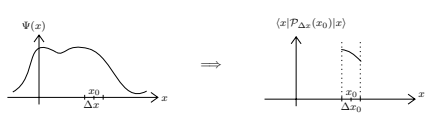
\includegraphics{immagini/19_image_2.png}
\end{center}
	
Le figure soprastanti mostrano cosa succede alla funzione d'onda. Prima della misura la funzione \'e nel suo stato iniziale $\Psi(x) = \braket{x}{\Psi}$ e ha come dominio tutto l'asse reale perch\'e la particella potr\'a trovarsi in qualsiasi punto; effettuando una misura ideale di prima specie il sistema \'e perturbato il meno possibile, per cui se la particella viene trovata all'interno dell'intervallo $\Delta x_0$, la funzione d'onda avr\'a la stessa forma precedente in quell'intervallo, mentre nella regione esterna collasser\'a a 0 (per cui dovr\'a essere rinormalizzata in accordo con l'interpretazione probabilistica di Born della funzione d'onda).
	

\begin{comment}
\subsubsection{Osservabili compatibili}
	
	Nel paragrafo precedente abbiamo considerato solamente osservabili a spettro non degenere, e abbiamo detto che immediatamente dopo la misura lo stato del sistema 'e completamente determinato perch´e 'e proiettato sull'autospazio relativo all'autovalore ak ∈ σd(A) trovato.
	
	Il caso non banale 'e quando ak 'e degenere, infatti dopo la misura possiamo solamente sapere che lo stato del sistema sta nell'autospazio multidimensionale relativo ad ak. Quindi per determinare univocamente lo stato 'e necessario misurare altre grandezze fisiche, con il requisito che non deteriorino l'informazione acquisita misurando A, ma anzi, la migliorino. Le osservabili per cui questo succede sono dette *osservabili compatibili* con A. Diamone la definizione operativa:
	Definizione 4. Immaginiamo che A e B siano grandezze fisiche a spettro discreto. Al tempo t *effettuiamo* una misura di A e otteniamo il risultato ak ∈ σd(A); subito dopo, cio'e prima che il sistema possa evolvere temporalmente in modo non banale, al tempo t
	+ facciamo una misura di B *ottenendo il risultato* bi ∈ σd(B),
	allora B 'e compatibile con A se ripetendo la misura di A *all'istante* t
	++ *otteniamo con certezza il valore* ak,
	∀ak, bi e ∀ *stato (cio'e non deve essere una particolare coincidenza).*
	Vediamo come tradurre nel linguaggio matematico della MQ questo risultato. Enunciamo e dimostriamo a tal proposito due teoremi.
	
	Teorema 1.3.1. A e B sono due osservabili compatibili ⇐⇒ *esiste una base ortonormale di autovettori comuni,*
	cio'e simultaneamente autovettori di A e B.
	
	Dimostrazione. =⇒: sappiamo che A e B essendo associati ad osservabili sono operatori autoaggiunti, allora qualsiasi vettore dello spazio di Hilbert pu'o essere decomposto in autostati dell'operatore A perch´e esiste sempre una base ortonormale di autovettori di questo operatore per H
	
	$$|\Psi\rangle=\sum_{a_{k}\in\sigma(A)}|\Psi_{a_{k}}\rangle$$
	
	in cui |\Psiak i 'e la proiezione del vettore sugli autospazi. Questo 'e ovviamente vero anche per l'operatore B
	
	$$|\Psi_{a_{k}}\rangle=\sum_{b_{i}\in\sigma(B)}|\Psi_{b_{i}}(a_{k})\rangle$$
	
	In generale se A e B sono operatori autoaggiunti qualsiasi, gli |\Psibi
	,(ak)i non rimangono pi'u autovettori dell'operatore A, questo per'o si verifica se A e B sono osservabili compatibili, quindi in questo caso sono loro autostati simultanei e li scriviamo come |\Psiak,bi i. Allora possiamo riscrivere il vettore come
	
	$\Psi\rangle=\sum_{a_{k}\in\sigma(A),b_{i}\in\sigma(B)}\Psi_{a_{k},b_{i}}\rangle\qquad\forall\,|\Psi\rangle\in\mathcal{H}$.  
	Se non c''e degenerazione, cio'e l'intersezione degli autospazi relativi ad ak e bi 'e unidimensionale, abbiamo concluso la dimostrazione; se invece c''e degenerazione, 'e sufficiente decomporre ogni autovettore all'interno degli autospazi di dimensione maggiore di 1 come |\PsiΦak,pi,τ i, e aggiungere una somma sull'indice τ che conta la degenerazione.
	
	⇐=: A e B possiedono una base di autovettori comuni |\Psiak,bi,τ i, allora il generico stato \Psi si pu'o decomporre in
	
	$$|\Psi\rangle=\sum_{a_{k},b_{i},\tau}c_{a_{k},b_{i},\tau}\left|\Psi_{a_{k},b_{i},\tau}\right\rangle$$
	
	Quello che fa la misura dell'osservabile A 'e eliminare la sommatoria sul suo spettro dato che 'e stato trovato solamente il valore ak, cio'e seleziona la proiezione ortogonale sull'autospazio relativo all'autovalore ak. Succede lo steso se effettuiamo la misura di B e otteniamo come risultato bi
	
	misura di $A\to\quad\sum_{b_{i},\tau}c_{a_{k},b_{i},\tau}\,|\,\Psi_{a_{k},b_{i},\tau}\rangle$ misura di $B\to\quad\sum_{\tau}c_{a_{k},b_{i},\tau}\,|\,\Psi_{a_{k},p_{i},\tau}\rangle$
	quindi resta solamente la somma sulla degenerazione residua. Ovviamente questi autovettori appartengono all'autospazio di A relativo all'autovalore ak, quindi effettuando una nuova misura di A non possiamo che trovare ak, e questa 'e esattamente la definizione che abbiamo dato per A e B osservabili compatibili.
	
	Un modo equivalente per enunciare questo risultato 'e di dire che se due osservabili sono compatibili possiamo decomporre l'intero spazio di Hilbert come la somma diretta degli autospazi relativi ai due operatori Hak,bi =
	Hak ∩ Hbi
	
	$$\mathcal{H}=\bigoplus_{a_{k}\in\sigma(A),b_{i}\in\sigma(B)}\mathcal{H}_{a_{k},b_{i}}$$
	$\texttt{1.3.2}$
	Inoltre questo teorema si pu'o estendere anche a operatori con spettro continuo, ricordando di considerare il problema agli autovalori generalizzato nello spazio delle distribuzioni, e di rimpiazzare le somme con gli integrali.
	
	Teorema 1.3.2. A e B sono due osservabili compatibili ⇐⇒ commutano tra loro, cio'e [*A, B*] = 0.
	
	Dimostrazione. =⇒: facciamo agire AB sul generico stato |\Psii e sfruttiamo il risultato del teorema precedente considerando una base di autovettori comuni di A e B
	
	$$AB\left|\Psi\right\rangle=AB\sum_{a_{k}\in\sigma(A),b_{i}\in\sigma(B)}\left|\Psi_{a_{k},b_{i}}\right\rangle=\sum_{a_{k},b_{i}}a_{k}b_{i}\left|\Psi_{a_{k},b_{i}}\right\rangle=\sum_{a_{k},b_{i}}b_{i}a_{k}\left|\Psi_{a_{k},b_{i}}\right\rangle$$ $$=A\sum_{a_{k},b_{i}}b_{i}\left|\Psi_{a_{k},b_{i}}\right\rangle=BA\sum_{a_{k},b_{i}}\left|\Psi_{a_{k},b_{i}}\right\rangle=BA\left|\Psi\right\rangle\quad\longrightarrow\quad[A,B]=0$$
	
	⇐=: dato che A 'e autoaggiunto possiamo decomporre lo spazio di Hilbert nella somma dei suoi autospazi H =Lak∈σ(A) Hak
	, quindi prendendo un qualsiasi vettore |\Psiak i ∈ Hak vale la seguente catena di uguaglianze
	
	$$A B\left|\Psi_{a_{k}}\right\rangle=B A\left|\Psi_{a_{k}}\right\rangle=B a_{k}\left|\Psi_{a_{k}}\right\rangle=a_{k}\big(B\left|\Psi_{a_{k}}\right\rangle\big)$$
	$$\square$$
	
	abbiamo ottenuto che B |\Psiak i 'e autostato di A relativo all'autovalore ak, cio'e Hak
	'e invariante sotto l'azione di B. Possiamo quindi considerare la restrizione di B che agisce su Hak e che rimane un operatore autoaggiunto:
	
	$$\mathcal{H}_{a_{k}}=\bigoplus_{b_{i}\in\sigma(B)}\mathcal{H}_{a_{k},b_{i}}\qquad\longrightarrow\qquad\mathcal{H}=\bigoplus_{a_{k}\in\sigma(A),b_{i}\in\sigma(B)}\mathcal{H}_{a_{k},b_{i}}$$
	
	Anche in questo caso il teorema si pu'o estendere facilmente al caso continuo con il consueto metodo.
	
	Se A e B sono limitati questo teorema 'e valido rigorosamente perch´e gli operatori possono essere definiti in tutto H, per cui D(A) = D(B) = D(AB) = D(BA). Per operatori illimitati ci possono essere casi patologici/particolari con problemi di dominio che non considereremo mai.
	
	Introduciamo ora un concetto molto importante per lo studio di un sistema quantistico: l'*insieme completo di* osservabili compatibili, chiamato pi'u semplicemente *ICOC*. La caratteristica di questo set di osservabili 'e che se effettuiamo una loro misura simultanea, identifichiamo il sistema in modo univoco, senza l'ambiguit'a che era presente nel caso dello spettro degenere.
	
	Definizione 5. *Consideriamo un vettore di N grandezze fisiche misurabili* A~ = (A1, ..., AN ) a cui associamo i rispettivi operatori A~ = (A1, A2, ..., AN ) *a spettro discreto. Supponiamo che queste osservabili siano compatibili* tra loro, e facciamo una misura di prima specie ottenendo come risultato il vettore ~a = (a1, ..., aN )*; sappiamo che* lo spazio HA = Ha1,...,aN sar'a dato dall'intersezione degli autospazi delle osservabili relativi ai diversi autovalori.
	
	Le osservabili saranno un ICOC se questo autospazio 'e non degenere, cio'e se ha dimensione unitaria.
	
	In generale, un insieme di osservabili deve verificare le seguenti due propriet'a per essere un ICOC: gli operatori commutano tra loro, e specificare un insieme di autovalori trovati con le misure determina univocamente lo stato del sistema. Quindi un modo equivalente per dire che un insieme di osservabili compatibili 'e completo 'e dire che esiste un'unica base ortonormale (a meno di fattori di fase) costituita tutta di autovettori simultanei di tutti gli operatori che costituiscono l'ICOC.
	
	Facciamo un esempio concreto. Per una particella priva di spin in una dimensione spaziale, X 'e un ICOC,
	perch´e sappiamo che esiste una base ortonormale generalizzata priva di degenerazione di oggetti del tipo ξx0
	(x) = δ(x−x0) per la quale 'e possibile scrivere qualsiasi stato del sistema. Allo stesso modo P 'e ICOC perch´e conoscere la decomposizione della trasformata di Fourier della funzione d'onda nello spazio delle P equivale ad avere l'informazione completa sullo stato del sistema. Si pu'o dimostrare che l'hamiltoniamo non 'e un ICOC,
	perch´e 'e quadratico nelle P, quindi per ogni valore di energia abbiamo una duplice degenerazione dello spettro delle onde piane, risulta quindi necessario un altro operatore, per esempio P, che ci permette di rimuovere tale degenerazione conoscendo il segno del momento.
	
	Avere un ICOC ci consente di dare una rappresentazione degli stati in termini di opportune funzioni d'onda.
	
	Prendiamo l'esempio precedente, H = L2(R) e X e P che sono due ICOC separatamente, con base generalizzata di vettori che soddisfano alle equazioni astratte in 1.4 Ogni elemento di H lo possiamo scrivere mediante le relazioni di completezza generalizzate per lo spettro continuo
	
	$$|\Psi\rangle=\int\mathrm{d}x\,|x\rangle\underbrace{\langle x|\Psi\rangle}_{\Psi(x)}\qquad\qquad|\Psi\rangle=\int\mathrm{d}p\,|p\rangle\underbrace{\langle p|\Psi\rangle}_{\Psi(p)}$$
	
	Pi'u in generale, possiamo applicare questo ragionamento a qualsiasi ICOC A~ con autovettori |~ai, i quali formano una base generalizzata per H, allora la decomposizione del ket |\Psii 'e del tutto analoga ai casi specifici precedenti
	
	$$|\Psi\rangle=\int\mathrm{d}\vec{a}\,|\vec{a}\rangle\underbrace{\langle\vec{a}|\Psi\rangle}_{\Psi(\vec{a})}$$
\end{comment}


\begin{comment}
	

# Capitolo 2 Evoluzione Temporale (O Causale) Di Un Sistema Quantistico

Abbiamo gi'a detto che in MQ si perde il determinismo che invece caratterizza la MC, cio'e in certe situazioni non
'e possibile prevedere esattamente il risultato di una misura ma al massimo la probabilit'a che una data misura dia un risultato particolare. Questo non ha nulla a che vedere con l'evoluzione temporale di un sistema che si trova in uno stato puro e isolato, infatti in questo caso c''e determinismo assoluto (causalit'a) e siamo in grado di calcolare esattamente quale sar'a lo stato del sistema ad un istante di tempo successivo t. Questo non significa che a quell'istante siamo in grado di misurare precisamente tutte le osservabili fisiche, perch´e per queste varr'a ancora l'interpretazione probabilistica.

Postulato 7. *Evoluzione temporale del sistema* Esiste un operatore H autoaggiunto associato all'energia totale del sistema che controlla l'evoluzione temporale attraverso l'equazione di Schr¨odinger dipendente dal tempo, che nello spazio di Hilbert astratto si scrive come

$$i\hbar{\frac{\partial\left|\Psi(t)\right\rangle}{\partial t}}=H(t)\left|\Psi(t)\right\rangle$$
$$(2.1)$$
∂t = H(t)|Ψ(t)i (2.1)
Quindi in questo approccio l'evoluzione temporale 'e parametrizzata dal modo in cui il vettore di stato dipende dalla coordinata temporale.

Ricordiamo che come conseguenza dell'equazione di Schr¨odinger abbiamo la conservazione della probabilit'a nel tempo, che in prima battuta si legge come il fatto che la norma degli stati non dipende dal tempo. Possiamo dimostrare questa affermazione abbastanza facilmente restando in una dimensione:

$$\frac{\mathrm{d}}{\mathrm{d}t}\left\langle\Psi(t)|\Psi(t)\right\rangle=\left(\frac{\mathrm{d}}{\mathrm{d}t}\left\langle\Psi(t)|\right\rangle|\Psi(t)\right)+|\Psi(t)\rangle\left(\frac{\mathrm{d}}{\mathrm{d}t}\left\langle\Psi(t)|\right\rangle\right)$$ $$=+\frac{i}{\hbar}\Big{(}\left\langle\,H\Psi(t)|\Psi(t)\right\rangle-\left\langle\Psi(t)|H\Psi(t)\right\rangle\,\Big{)}=0$$ $$\left\langle\Psi(t)|\Psi(t)\right\rangle=\left\langle\Psi(t_{0})|\Psi(t_{0})\right\rangle$$

in cui abbiamo moltiplicato e diviso per la quantit'a i~

in modo da poter scrivere l'operatore hamiltoniano, che
ricordiamo essere autoaggiunto. Ovviamente questo risultato vale anche nel caso tridimensionale, per il quale
definiamo:
$$\begin{array}{r l}{P({\vec{x}},t)={\frac{|\Psi({\vec{x}},t)|^{2}}{||\Psi||^{2}}}}&{{}{\mathrm{~dense}}}\\ {d w({\vec{x}},t)=\rho({\vec{x}})\,\mathrm{d}^{3}{\vec{x}}}\\ {W=\int\mathrm{d}^{3}x\,\rho({\vec{x}},t)=1}&{{}{\mathrm{~pair}}}\end{array}$$
||Ψ||2 densit'a di probabilit'a relativa alla posizione ~x
dw(*~x, t*) = ρ(~x) d3~x densit'a di probabilit'a infinitesima
3x ρ(*~x, t*) = 1 probabilit'a totale indipendente dal tempo
Vediamo come si pu'o scrivere la conservazione della probabilit'a. Consideriamo la forma generale dell'hamiltoniana
data dall'equazione 1.5 in cui per'o il potenziale dipende dal tempo
$$H={\frac{\vec{P}^{2}}{2m}}+V(\vec{X},t)$$
$$(2.2)$$
+ V (*X, t* ~ ) (2.2)
se la esplicitiamo nello spazio delle coordinate otteniamo l'equazione di Schr¨odinger dipendente dal tempo, di cui scriviamo anche la complessa coniugata:

$$i\hbar\frac{\partial}{\partial t}\Psi(\vec{x},t)=-\frac{\hbar^{2}}{2m}\vec{\nabla}^{2}\Psi(\vec{x},t)+V(\vec{x},t)\Psi(\vec{x},t)\qquad\qquad-i\hbar\frac{\partial}{\partial t}\Psi^{*}(\vec{x},t)=-\frac{\hbar^{2}}{2m}\vec{\nabla}^{2}\Psi^{*}(\vec{x},t)+V(\vec{x},t)\Psi^{*}(\vec{x},t)$$

moltiplichiamo la prima equazione per Ψ∗e la seconda per Ψ e sottraiamo membro a membro

$$i\hbar(\underbrace{\dot{\Psi}\Psi^{*}+\Psi\dot{\Psi}^{*}}_{\frac{\partial\rho}{\partial t}})=-\underbrace{\frac{\hbar}{2m}(\Psi^{*}\vec{\nabla}^{2}\Psi-\Psi\vec{\nabla}^{2}\Psi^{*})}_{\mathrm{(for~}}.$$

∂t
$\lambda^{\frac{1}{2}}$
$\phi$
$$\mathbf{\hat{\Pi}}^{+}$$
hΨ|Ψi = hUΨ|UΨi = |λ|
2hΨ|Ψ*i ⇐⇒ |*λ| = 1
| {z }
$$-{\dot{\vec{\nabla}}}J$$
La conservazione della probabilit'a assume le sembianze di una formula gi'a vista nel caso elettromagnetico, cio'e
l'equazione di continuit'a della corrente
$${\frac{\partial\rho}{\partial t}}+\vec{\nabla}\vec{j}(\vec{x},t)=0$$

## 2.1 Operatori Unitari

Definizione 6. Un operatore U nello spazio di Hilbert H *associato al nostro sistema quantistico, si dice unitario* se sono soddisfatte le seguenti due condizioni:
- 'e isometrico, ovvero conserva il prodotto scalare ∀ |Ψi, |Φi hUΨ|UΦi = hΨ|Φi
- *dominio e codominio coincidono con lo spazio di Hilbert* D(U) = C(U) = H
Data questa definizione di operatore unitario (non 'e l'unica, per esempio i matematici dicono che 'e sufficiente che dominio e codominio siano densi in H), derivano alcune importanti propriet'a che rendono questi operatori fondamentali nello studio dei sistemi in MQ:
1. U ammette un inverso U
−1: questa dimostrazione scaturisce automaticamente una volta verificato che la relazione |Ψ*i −→* U |Ψi 'e biunivoca, cio'e che U |Ψi = U |Φ*i −→ |*Ψi = |Φi

U |Ψi = U |Φi
$\langle U\Psi-U\Phi|U\Psi-U\Phi\rangle=\langle U\Psi|U\Psi\rangle+\langle U\Phi|U\Phi\rangle-\langle U\Phi|U\Psi\rangle-\langle U\Psi|U\Phi\rangle$  $\langle\Psi|\Psi\rangle+\langle\Phi|\Phi\rangle-\langle\Phi|\Psi\rangle-\langle\Psi|\Phi\rangle=\langle\Psi-\Phi|\Psi-\Phi\rangle=||\,|\Psi-\Phi\rangle\,||^{2}\longrightarrow|\Psi\rangle=|\Phi\rangle$
quindi esiste un inverso ed 'e evidente che anche questo 'e unitario, 2. U 'e lineare: definiamo il vettore |Ψi = α1 |Ψ1i + α2 |Ψ2i e dimostriamo che l'azione di U su |Ψi 'e lineare.

Prendendo un qualsiasi |Φ*i ∈ H* possiamo scrivere la seguente catena di uguaglianze

hΦ|UΨi =U
$$\begin{array}{l}{{\left\langle U^{-1}\Phi\right|\Psi\rangle=\left\langle U^{-1}\Phi\right|\left(\alpha_{1}\left|\Psi_{1}\right.\right)+\alpha_{2}\left|\Psi_{2}\right.\right\rangle}}\\ {{\left.\alpha_{1}\left\langle U^{-1}\Phi\right|\Psi_{1}\right\rangle+\alpha_{2}\left\langle U^{-1}\Phi\right|\Psi_{2}\right\rangle=U\big(\alpha_{1}\left.\left\langle\Phi\right|\Psi_{1}\right\rangle+\alpha_{2}\left.\left\langle\Phi\right|\Psi_{2}\right\rangle\big)}}\end{array}$$
= α1 Da quanto detto finora si estrapola che U
+ = U
−1,

3. U 'e limitato:
$$\langle U\Psi|U\Psi\rangle=\left\langle U^{+}U\Psi\right|\Psi\rangle=\langle\Psi|\Psi\rangle$$
ed essendo un operatore anche lineare, 'e continuo nello spazio di Hilbert.

4. gli autovalori di U hanno modulo unitario: detto |Ψi un autovettore di U associato all'autovalore λ:

5. due autovettori di U unitario corrispondenti ad autovalori distinti sono ortogonali: detti |Ψ1i e |Ψ2i
autovettori relativi a λ1, λ2, con λ1 6= λ2:
$$\langle\Psi_{1}|\Psi_{2}\rangle=\langle U\Psi_{1}|U\Psi_{2}\rangle=\lambda_{1}^{*}\lambda_{2}\,,$$
−→ (1 − λ
∗
1λ2)hΨ1|Ψ2i = 0 *⇐⇒ h*Ψ1|Ψ2i = 0
$$\lambda_{1}^{*}\lambda_{2}\neq1$$
$$\begin{array}{l l l}{{\theta_{2}\rangle=\lambda_{1}^{*}\lambda_{2}\left\langle\Psi_{1}|\Psi_{2}\right\rangle}}&{{}}&{{|\lambda_{1}|=|\lambda_{2}|=1}}&{{\quad m a}}\end{array}$$
Un modo equivalente per caratterizzare un operatore unitario 'e dire che il prodotto con il suo aggiunto (sia a destra che a sinistra) restituisce l'unit'a U
+U = UU + = 1 (2.3)
se ci capitasse di dover verificare con questa equazione che un operatore sia unitario, in uno spazio di dimensione finita basta verificare che una delle due uguaglianze sia verificata, nel caso di spazi con dimensione infinita devono essere verificate entrambe.

## 2.2 Evoluzione Temporale In Visuale Di Schr¨Odinger

La visuale di Schr¨odinger della MQ si focalizza sullo studio dell'evoluzione degli stati del sistema, quindi
matematicamente dei vettori espressi sottoforma di ket che li descrivono. Il punto di partenza per la discussione
dell'operatore di evoluzione temporale 'e l'equazione agli autovalori dipendente dal tempo che abbiamo scritto
in 2.1, in cui supponiamo che l'hamiltoniana abbia una dipendenza esplicita dal tempo (questo 'e il caso pi'u
generale, se non fosse cos'ı i risultati si semplificherebbero notevolmente). Questa 'e un'equazione differenziale al primo ordine nella coordinata temporale, quindi per determinare univocamente una sua soluzione serve una sola
condizione al contorno che 'e il vettore di stato all'istante iniziale t0. Inoltre 'e lineare ed omogenea nel vettore
|Ψ(t)i, questo significa che vale il principio di sovrapposizione, esattamente come ci aspettiamo.
La mappa |Ψ(t0)*i → |*Ψ(t)i definisce un operatore lineare U = U(*t, t*0) che 'e appunto l'*operatore di evoluzione*
temporale:
$$|\Psi(t)\rangle=U(t,t_{0})\,|\Psi(t_{0})\rangle\qquad\qquad U(t_{0},t_{0})=1\,.$$
Inserendo tale scrittura nell'equazione di Schr¨odinger, otteniamo l'equazione differenziale cui soddisfa questo
Instructions the covariant differentiation of conformal, Neumann curvature and structure on boundary operator: $$i\hbar\frac{\partial\left|\Psi(t)\right>}{\partial t}=H(t)\left|\Psi(t)\right>=i\hbar\frac{\partial}{\partial t}U(t,t_0)\left|\Psi(t_0)\right>=H(t)U(t,t_0)\left|\Psi(t_0)\right>\longrightarrow$$ $$\longrightarrow\quad i\hbar\frac{\partial U(t,t_0)}{\partial t}=H(t)U(t,t_0)\tag{2.4}$$  Integrando etotanimo un'altra exprescione che incorpera sia l'equatione diferenziale che la condicione inicialmente esta la transformada de la (2.4). 
$$\int_{t_{0}}^{t}\mathrm{d}t^{\prime}\,i\hbar\frac{\partial U(t^{\prime},t_{0})}{\partial t}=\int_{t_{0}}^{t}\mathrm{d}t^{\prime}\,H(t^{\prime})U(t^{\prime},t_{0})\quad\longrightarrow\quad i\hbar\big{(}U(t,t_{0})-1\big{)}=\int_{t_{0}}^{t}\mathrm{d}t^{\prime}\,H(t^{\prime})U(t^{\prime},t_{0})$$ $$U(t,t_{0})-1=-\frac{i}{\hbar}\int_{t_{0}}^{t}\mathrm{d}t^{\prime}\,H(t^{\prime})U(t^{\prime},t_{0})\tag{2.5}$$  Vediano un altra importante caracteristica dell'operatore di evoluzione temporale $U$. Ricerviamo la definiciones

che abbiamo dato inizialmente di stato evoluto come:
$$(2.4)$$
$$|\Psi(t)\rangle=U(t,t^{\prime})\,|\Psi(t^{\prime})\rangle$$
nulla ci vieta di considerare |Ψ(t 0)i come l'evoluzione di un altro stato |Ψ(t 00)i mediante lo stesso operatore, ma dipendente da degli opportuni parametri:

$$|\Psi(t^{\prime})\rangle=U(t^{\prime},t^{\prime\prime})\,|\Psi(t^{\prime\prime})\rangle$$

allora sostituendo all'equazione precedente otteniamo una formula per l'evoluzione considerando step intermedi, che deve necessariamente essere uguale a quella globale senza frammentazione dell'asse temporale

$\Psi(t)\rangle=U(t,t^{\prime})U(t^{\prime},t^{\prime\prime})\,|\Psi(t^{\prime\prime})\rangle\quad\stackrel{{!}}{{=}}U(t,t^{\prime\prime})\,|\Psi(t^{\prime\prime})\rangle\quad\longrightarrow\quad U(t,t^{\prime\prime})=U(t,t^{\prime})U(t^{\prime},t^{\prime\prime})$.  
questa relazione ha un importante significato: l'evoluzione temporale dipende solamente dagli istanti iniziale e
finale considerati, non dal valore assoluto dell'intervallo temporale in questione; in particolare se poniamo in
questa formula t
00 = t, dall'equazione 2.3 risulta:
$$\mathbb{1}=U(t,t^{\prime})U(t^{\prime},t)=U(t^{\prime},t)U(t,t^{\prime})\quad\longrightarrow\quad U(t,t^{\prime})=U^{-1}(t^{\prime},t)\quad\mathrm{in}\quad t^{\prime}=t^{\prime}.$$
0, t) inversione temporale
Chiediamoci ora cosa succede se l'intervallo temporale su cui consideriamo l'evoluzione 'e infinitesimo dt e
sviluppiamo l'equazione di Schr¨odinger per questo caso:
 Momente in non-singular par "quotee" $$\begin{array}{lcl}d\left|\Psi(t)\right>&=&\left|\Psi(t+dt)\right>-\left|\Psi(t)\right>=-\dfrac{i}{\hbar}H(t)\left|\Psi(t)\right>\mathrm{d}t\\ \text{risolvendo per}&\left|\Psi(t+dt)\right>&\\ &\left|\Psi(t+dt)\right>&=&\left(1-\dfrac{i}{\hbar}H(t)\right)\left|\Psi(t)\right>\stackrel{!}{=}U(t+dt,t)\left|\Psi(t)\right>\\ &U(t+dt,t)&=&\left(1-\dfrac{i}{\hbar}H(t)\right)dt\\ \end{array}$$ l'usquelizione di de operatori diveri como cojumolero derivate o integral. 

abbiamo riscritto l'uguaglianza di due operatori diversi senza coinvolgere derivate o integrali, quindi possiamo interpretare il secondo membro dell'ultima equazione come l'operatore che d'a l'evoluzione temporale del sistema per un tempo infinitesimo, in questo caso si dice che H 'e *generatore delle traslazioni temporali*. Poich´e H 'e autoaggiunto e definito in un dominio denso in H, esiste un teorema matematico che dice che il corrispondente operatore infinitesimo U 'e unitario, e da questo si pu'o dedurre sotto opportune ipotesi che anche l'operatore di evoluzione temporale per un intervallo di tempo finito 'e unitario:

$$U^{+}(t+dt,t)=\left(1+\frac{i}{\hbar}H(t)\right)\mathrm{d}t\quad\longrightarrow\quad UU^{+}=U^{+}U=1+\mathcal{O}\big{(}t^{2}\big{)}\quad\longrightarrow\quad U^{+}(t,t^{\prime})=U^{-1}(t,t^{\prime})=U(t^{\prime},t)$$

in cui abbiamo scartato i termini di ordine superiore al primo dato che lavoriamo con infinitesimi al primo ordine.

## 2.2.1 Evoluzione Temporale Per Sistemi Conservativi

I sistemi conservativi sono quelli per cui vale la conservazione dell'energia e in cui le forze che agiscono non dipendono dal tempo, di conseguenza nemmeno l'energia/hamiltoniana. Per questi sistemi il tempo 'e *omogeneo*, cio'e non non esiste un istante privilegiato (sono tutti equivalenti) e le leggi della fisica non dipendono dall'intervallo considerato, quindi facendo evolvere il sistema in intervalli di lunghezza uguale, ci aspettiamo che l'evoluzione temporale sia la stessa, cio'e che l'operatore U(*t, t*0) dipenda solamente da un'unica variabile τ = t − t0 e che continuino a valere le stesse propriet'a studiate al paragrafo precedente

$$U(\tau),\qquad U(0)=\mathbb{I}\,,\qquad U(\tau_{1})U(\tau_{2})=U(\tau_{1}+\tau_{2})$$
$$[U(\tau)]^{-1}=U(-\tau)$$
 $\begin{array}{cc}\left|\Psi(t)\right>=U(t-t_0)\left|\Psi(t_0)\right>&A(t)=A(t_0)\end{array}$  or $\grave{\lambda}$, the stati iniciali-diversi-damos-lucos-s-stat. 
Consideriamo l'equazione di Schr¨odinger per l'operatore U che abbiamo trovato in 2.4, ora l'hamiltoniana che compare 'e indipendente dal tempo e la soluzione 'e piuttosto semplice da trovare avendo a disposizione la
condizione iniziale
$$i\hbar{\frac{\mathrm{d}}{\mathrm{d}\tau}}U(\tau)=H U(\tau)\quad\longrightarrow\quad U(t-t_{0})=e^{-i{\frac{H}{\hbar}}(t-t_{0})}$$
dato che l'hamiltoniana 'e autoaggiunta, si pu'o dimostrare che questo operatore 'e unitario e definito su tutto H.
La caratteristica principale dell'evoluzione temporale nella visuale di Schr¨odinger, la si pu'o estrapolare osservando
quello che abbiamo fatto finora: gli stati evolvono mediante l'operatore U(τ ) ma le osservabili/operatori/strumenti
di misura restano fisse:
|Ψ(t)i = U(t − t0)|Ψ(t0)i A(t) = A(t0) (2.6)
Un fatto importante da notare 'e che stati iniziali diversi danno luogo a stati finali diversi, questo perch´e
l'evoluzione temporale 'e una mappa invertibile quindi non deve presentare punti di intersezione tra curve
differenti
$$|\Psi(t_{0})\rangle\neq|\Phi(t_{0})\rangle\quad\longrightarrow\quad|\Psi(t)\rangle\neq|\Phi(t)\rangle$$
le traiettorie nello spazio delle fasi devono essere sempre distinte e non devono intersecarsi per non incappare in ambiguit'a nel momento in cui invertiamo la relazione, cio'e la mappa dev'essere biettiva.
Consideriamo ora uno stato qualsiasi in un istante iniziale |Ψ(t0)i; la ricetta appena trovata ci suggerisce
che l'evoluzione causale 'e data da
$$|\Psi(t)\rangle=e^{-i{\frac{H}{\hbar}}(t-t_{0})}\,|\Psi(t_{0})\rangle$$
(t−t0)|Ψ(t0)i (2.7)
Proviamo a trovare la scrittura esplicita in termini degli autostati dell'hamiltoniana |En, rni (sappiamo che
essendo una base ortonormale vale hEn, rn|Em, rmi = δmn, con rn l'indice che conta la degenerazione). Quello
che dobbiamo fare 'e decomporre lo stato iniziale e scriverlo come combinazione degli autovettori:
$$(2.6)$$
$$(2.7)$$
$$|\Psi(t_{0})\rangle=\sum_{E_{n}\in\sigma(H)}\sum_{r_{n}}|E_{n},r_{n}\rangle\left\langle E_{n},r_{n}|\Psi(t_{0})\right\rangle\quad\longrightarrow$$ $$\longrightarrow|\Psi(t)\rangle=\sum_{E_{n}\in\sigma(H)}e^{-\frac{i}{\hbar}E_{n}(t-t_{0})}\sum_{r_{n}}|E_{n},r_{n}\rangle\left\langle E_{n},r_{n}|\Psi(t_{0})\right\rangle$$
$$(2.8)$$
Per il caso di spettro continuo si procede generalizzando la somma sugli autovalori discreti all'integrale sullo spettro continuo, con l'accortezza di mantenere la degenerazione discreta:

$$|\Psi(t_{0})\rangle=\int_{\sigma(H)}dE\sum_{r}|E,r\rangle\left\langle E,r|\Psi(t_{0})\right\rangle\quad\longrightarrow\quad|\Psi(t)\rangle=\int_{\sigma(H)}e^{-\frac{i}{\hbar}E(t-t_{0})}\sum_{r}|E,r\rangle\left\langle E,r|\Psi(t_{0})\right\rangle dE$$  Chiedamosj quando il valor medio di una grandeza fisica overvable non dipende del tempo. Consideremos
l'equazione di Schr¨odinger dipendente dal tempo e la sua complessa coniugata:
$$\begin{array}{r c l}{{\left[\begin{array}{c c}{{}}&{{i\hbar{\frac{\mathrm{d}\left|\Psi\right\rangle}{\mathrm{d}t}}=H\left|\Psi\right\rangle}}\\ {{}}&{{-i\hbar{\frac{\mathrm{d}\left|\Psi\right\rangle}{\mathrm{d}t}}=H\left\langle\Psi\right|}}\end{array}\right.}}&{{\longrightarrow}}&{{i\hbar{\frac{\mathrm{d}}{\mathrm{d}t}}\left\langle\Psi|A|\Psi\right\rangle=\left\langle\Psi|[A,H]|\Psi\right\rangle}}\end{array}$$

Ci sono due situazioni in cui la richiesta viene rispettata:
1. ∀Ψ quando [*A, H*] = 0, che corrisponde alla situazione in cui ci sono delle simmetrie dinamiche, cio'e la grandezza A 'e conservata.

2. ∀A se |Ψi 'e un autostato dell'hamiltoniano, cio'e 'e un cos'ı detto stato stazionario.

## 2.3 Trasformazioni Unitarie

Sono un particolare tipo di trasformazioni che a partire da un certo stato |Ψ(t)i forniscono |Ψ0(t)i, e a partire dall'operatore A forniscono A0; dunque agiscono sia sugli stati che sugli operatori. Dato un operatore U nello spazio di Hilbert H, la trasformazione unitaria 'e definita come

$$\forall\left|\Psi\right\rangle\quad\left|\Psi^{\prime}\right\rangle=U\left|\Psi\right\rangle$$
$$\forall A\quad A^{\prime}=U A U^{+}$$
0i = U |Ψi ∀A A0 = UAU +
Le trasformazioni unitarie costituiscono delle simmetrie del formalismo, ma non dinamiche perch´e a priori non lasciano invariata l'hamiltoniana e non implicano che le equazioni della dinamica mantengono la stessa forma; significano semplicemente che esistono diversi modi equivalenti per descrivere la stessa fisica.

Le trasformazioni unitarie lasciano invariati:
- i prodotti scalari: hΦ
0|Ψ0i = hUΦ|UΨi = hΦ|Ψi
- gli elementi di matrice: hΦ
0|A0|Ψ0i = hUΦ|UAU +|UΨi = hΦ|U
+UAU +U|Ψi = hΦ|A|Ψi
- la condizione di autoaggiuntezza degli operatori: A = A+ −→ (A0)
+ = (UAU +)
+ = UAU + = A+
- lo spettro delle osservabili: A0|a 0 k i = UAU +U |aki = akU |aki = ak |a 0 k i
- le relazioni algebriche tra gli operatori: AB = C A0B0 = UAU +UBU + = UABU + = UCU + = C
0 Ci sono delle precisazioni da fare su questo tipo di trasformazioni. La prima 'e che non stiamo parlando di evoluzione temporale, nonostante abbiamo scelto di usare lo stesso simbolo, infatti come sappiamo quest'ultima evolve o gli stati o le osservabili separatamente, mentre qui stiamo trasformando entrambe queste entit'a contemporaneamente. Inoltre le trasformazioni unitarie non esauriscono tutte le simmetrie del formalismo della MQ che soddisfano alle richieste che abbiamo appena elencato, pi'u avanti introdurremo delle trasformazioni dette antiunitarie che realizzano quanto abbiamo appena detto e che si differenziano da quelle unitarie per la antilinearit'a.

## 2.4 Evoluzione Temporale In Visuale Di Heisenberg

Studiamo ora la versione complementare a quella di Schr¨odinger, cio'e la visuale di Heisenberg che ovviamente porta allo stesso risultato. Consideriamo sistemi conservativi in cui H non dipende dal tempo; nella visuale di Schr¨odinger sappiamo gi'a come trasformano lo stato |Ψ(t0)i e l'operatore A(t0) grazie alle relazioni in 2.6. Come si pu'o immaginare, nella visuale di Heisenberg succede l'opposto:

$$\Psi_{h}(t))=|\Psi(t_{0})\rangle A_{h}(t)=U(t_{0}-t)A(t_{0})U^{+}(t_{0}-t)=[U(t-t_{0})]^{+}A(t_{0})U(t-t_{0})\tag{2.9}$$

Dato che descrivono la stessa fisica, queste due visuali devono essere legate da una trasformazione unitaria che 'e evidente essere la trasformazione generata dall'operatore unitario di traslazione temporale, allora

$$|\Psi(t)\rangle_{s}=U(t-t_{0})\,|\Psi(t_{0})\rangle$$
|Ψ(t)is = U(t − t0)|Ψ(t0)i As(t) = U(t − t0)Ah(t)U
$$A_{s}(t)=U(t-t_{0})A_{h}(t)U^{+}(t-t_{0})$$

in cui Hs = Hh perch´e l'operatore U 'e scritto in funzione dell'hamiltoniana stessa e quindi commuta con essa.

Cerchiamo ora di ricavare l'equazione di Heisenberg, cio'e l'equivalente dell'equazione differenziale di Schr¨odinger che determina l'evoluzione temporale dell'osservabile, in cui l'operatore A non 'e esplicitamente dipendente dal tempo.

d dt |Ψh(t)i = 0 per gli stati i~ d dt Ah(t) = i~ d dt U +(t − t0)AsU(t − t0) = i~ dU +(t − t0) dtAsU(t − t0) + i~U +(t − t0)As dU(t − t0) dt ricordando che i~ d dt U(t − t0) = HU(t − t0) = −U +(t − t0)HAsU(t − t0) + U +(t − t0)AsHU(t − t0) = U +(t − t0)AsU(t − t0) · H − H · U +(t − t0)AsU(t − t0) = [Ah, H] i~ dA(t)h dt= [Ah, H] equazione di Heisenberg (2.10)
$$(2.10)$$
Se consideriamo grandezze fisiche con dipendenza esplicita dal tempo As(t) = As(*q, p, ..., t*), l'equazione di Heisenberg acquista un termine aggiuntivo ed 'e facile dimostrare che assume la seguente forma:

$$i\hbar{\frac{\mathrm{d}A_{h}(t)}{\mathrm{d}t}}=[A_{h},H]-i\hbar\left[{\frac{\partial A(t)}{\partial t}}\right]_{h}\qquad\qquad\mathrm{con}\quad{\frac{\partial A_{s}(t)}{\partial t}}=i\hbar U^{+}(t-t_{0}){\frac{\partial A_{h}(t)}{\partial t}}U(t-t_{0})$$

Questo 'e quanto ci serve per discutere l'evoluzione temporale in visuale di Heisenberg di sistemi indipendenti dal tempo.

## 2.4.1 Evoluzione Temporale Per Sistemi Non Conservativi

Discutiamo ora il caso generale in cui estendiamo la dipendenza degli operatori anche dalla coordinata temporale esplicitamente. Riprendiamo la formula integrale che avevamo trovato per l'operatore U(*t, t*0) nell'equazione 2.5:
se l'hamiltoniana fosse indipendente dal tempo la soluzione di questo problema sarebbe banale, quindi escludiamo questo caso e risolviamo l'equazione pi'u complessa con un procedimento iterativo, notando che l'operatore U 'e presente in entrambi i membri. In questo caso l'hamiltoniana viene trattata come il parametro su cui espandere e il risultato all'ordine successivo si trova inserendo il precedente nell'equazione generale:

U (0) = 1 U (1) = 1 − i~ R t t0 dt1H(t1) U (2) = 1 − i ~ Z t t0 dt1H(t1) +− i~ 2 R t t0 dt1 R t1 t0 dt2H(t1)H(t2) | {z } U(t−t0) U (n)(t − t0) = U (n−1)(t − t0) + − i~ nZ t t0 Z t1 t0 ... Z tn−1 t0 | {z } n volte dtn H(t, t1)H(t, t2)...H(t, tn) | {z } n volte

in cui stiamo implicitamente considerando la catena di disuguaglianze t0 < tn < tn−1 < ... < t2 < t1.

Possiamo arrivare a una forma molto pi'u simmetrica introducendo il *prodotto cronologico tra operatori*, che definiamo con l'operatore T tale per cui:

$$T H(t_{1})H(t_{2})\equiv\left\{\begin{array}{l l}{{H(t_{1})H(t_{2})}}&{{\mathrm{se}\ t_{2}<t_{1}}}\\ {{H(t_{2})H(t_{1})}}&{{\mathrm{se}\ t_{1}<t_{2}}}\end{array}\right.$$

notiamo subito che possiamo riscriverlo in termini della funzione gradino di Heaviside centrata nell'origine

$$\theta(t)=\left\{\begin{array}{l l l}{{1}}&{{\approx t>0}}\\ {{0}}&{{\approx t<0}}\end{array}\right.\quad\longrightarrow\quad T H(t_{1})H(t_{2})=\theta(t_{1}-t_{2})H(t_{1})H(t_{2})+\theta(t_{2}-t_{1})H(t_{2})H(t_{1})$$

L'introduzione di questo tipo di funzione 'e necessaria perch´e in generale le hamiltoniane valutate a istanti di tempo diversi non commutano tra loro. Dimostriamo che effettivamente vale l'uguaglianza

$$\int_{t_{0}}^{t}d t_{1}\int_{t_{0}}^{t_{1}}d t_{2}H(t_{1})H(t_{2})=\frac{1}{2}\int_{t_{0}}^{t}d t_{1}\int_{t_{0}}^{t}d t_{2}T H(t_{1})H(t_{2})\quad\quad\quad\quad t_{1}>t_{2}$$

![28_image_0.png](28_image_0.png)

Graficamente la regione in cui stiamo svolgendo il primo integrale 'e rappresentata dal triangolo che sta sopra la bisettrice in figura. Questo stesso integrale si pu'o scrivere in modo alternativo come

$$\int_{t_{0}}^{t}\mathrm{d}t_{2}\int_{t_{2}}^{t}\mathrm{d}t_{1}\,H(t_{1})H(t_{2})\qquad t_{1}>t_{2}\qquad\mathrm{o~anche~come}$$
$$\int_{t_{0}}^{t}\mathrm{d}t_{1}\int_{t_{1}}^{t}\mathrm{d}t_{2}\,H(t_{2})H(t_{1})\qquad t_{2}>t_{1}$$

Ora sfruttiamo le propriet'a della θ di Heaviside e estendiamo l'integrale a tutto il quadrato

$$\frac{1}{2}\left[\int_{t_{0}}^{t}\!\mathrm{d}t_{1}\int_{t_{1}}^{t}\!\mathrm{d}t_{2}\,\theta(t_{1}-t_{2})H(t_{1})H(t_{2})+\int_{t_{0}}^{t}\!\mathrm{d}t_{1}\int_{t_{1}}^{t}\!\mathrm{d}t_{2}\,\theta(t_{2}-t_{1})H(t_{2})H(t_{1})\right]=\frac{1}{2}\int_{t_{0}}^{t}\!\mathrm{d}t_{1}\int_{t_{0}}^{t}\!\mathrm{d}t_{2}\,TH(t_{1})H(t_{2})$$  Since $t_{0}$ is a constant, we can obtain a limit as a function of $t_{0}$ will be included.  
Se vogliamo essere pi'u precisi e considerare non solo i primi ordini, ma arrivare fino all'n-esimo, dobbiamo riformulare la definizione di prodotto cronologico in modo opportuno

$$\theta(t_{1},...t_{n})=\theta(t_{1}-t_{2})\theta(t_{2}-t_{3})...\theta(t_{n-1}-t_{n})\quad\longrightarrow\quad TH(t_{1})...H(t_{n})=\sum_{p}\theta(t_{p_{1}},...t_{p_{n}})H(t_{p_{1}})H(t_{p_{2}})...H(t_{p_{n}})$$

in cui p1, p2*, ..., p*n sono le permutazioni possibili della striscia (1, 2*, ..., n*); allora l'operatore di evoluzione temporale all'ordine n si scrive come:

$$U^{(n)}(t,t_{0})=U^{(n-1)}+\frac{1}{n!}\left(-\frac{i}{\hbar}\right)^{n}\int_{t_{0}}^{t}\mathrm{d}t_{1}\int_{t_{0}}^{t}d t t_{2}...\int_{t_{0}}^{t}\mathrm{d}t_{n}\,H(t_{1})H(t_{2})...H(t_{n})\,.$$

formalmente questa 'e una serie esponenziale (non 'e garantito che converga), allora in notazione sintetica possiamo scrivere l'espressione formale dell'operatore di evoluzione temporale nel caso in cui l'hamiltoniana dipenda dal tempo

$$U(t,t_{0})=T e^{-{\frac{i}{\hbar}}\int_{t_{0}}^{t}\mathrm{d}t^{\prime}H(t^{\prime})}$$

## 2.5 Limite Classico E Teorema Di Ehrenfest

Naturalmente tutto quello che abbiamo detto finora deve essere concorde con quanto viene accettato dalla teoria della MC, dunque nel limite in cui il parametro caratterizzante la MQ (cio'e ~ opportunamente definito) tende a 0, dobbiamo ritrovare le equazioni classiche, e in particolare quelle di Hamilton per l'evoluzione delle osservabili.

Per studiare il comportamento della MQ nel limite classico, consideriamo come al solito una particella priva di spin in una dimensione, lavoriamo in visuale di Heisenberg e dunque partiamo dalla sua equazione generale trovata in 2.10 per un operatore autoaggiunto A = A(*Q, P*) = f(*Q, P*), che sia funzione di Q e P ma non esplicitamente del tempo. Abbiamo sempre considerato l'hamiltoniana come funzione di P e Q della forma H = H(*Q, P*) = P
2 2m + V (Q), adesso facciamo una piccola semplificazione e consideriamola come un polinomio

$$H=\sum_{m,n}a_{m n}P^{m}Q^{n}=\sum_{m,n}a_{m n}(P^{n}Q^{m}+Q^{m}P^{n})$$

in cui abbiamo preso una combinazione simmetrica di QP per essere coerenti con la MC e il principio di simmetrizzazione. Manipoliamo tale scrittura calcolando alcuni commutatori

$$[Q,H]=QH-HQ=\sum_{m,n}a_{mn}\big{(}QP^{n}Q^{m}+Q^{m}QP^{n}-P^{n}QQ^{m}-Q^{m}P^{n}Q\big{)}=0$$  $$\sum_{m,n}a_{mn}\big{(}[Q,P^{n}]Q^{m}+Q^{m}[Q,P^{n}]\big{)}=\sum_{m,n}a_{mn}\big{\{}[Q,P^{n}],Q^{m}\big{\}}$$

(Q e Qm commutano, quindi possiamo invertire l'ordine di applicazione) sapendo che vale: [*Q, f*(P)] =
i~
df(P )
dP −→ [*Q, P* n] = i~
dP
n dP[*P, Q*m] = −i~
dQm dQ
:

$$[Q,H]=\sum_{m,n}a_{m n}\left\{i\hbar\frac{\mathrm{d}P^{m}}{\mathrm{d}P},Q^{m}\right\}=i\hbar\sum_{m,n}a_{m n}\frac{\mathrm{d}}{\mathrm{d}P}\{P^{n},Q^{m}\}=i\hbar\frac{\partial H}{\partial P}$$
Un risultato simetrico si troya per $[P,H].$ Otteniano facilement I'evoluzone degli operator $$i\hbar\frac{\mathrm{d}Q}{\mathrm{d}t}=[Q,H]=i\hbar\frac{\partial H}{\partial P}\qquad\qquad\qquad i\hbar\frac{\mathrm{d}P}{\mathrm{d}t}=[P,H]=-i\hbar\frac{\partial H}{\partial Q}$$. 
La conclusione 'e immediata, infatti notiamo subito che queste due equazioni sono formalmente identiche alle equazioni canoniche di Hamilton dell'equazione 1.1; presentano per'o una differenza sostanziale: in MC abbiamo funzioni numeriche reali del tempo, in MQ abbiamo a che fare con operatori autoaggiunti dipendenti dal tempo, quindi per stabilire una corrispondenza biunivoca dobbiamo aggiungere qualcosa alla nostra trattazione.

Consideriamo un pacchetto d'onda abbastanza stretto in modo che rappresenti al meglio una particella classica, e uno stato generico Ψ; il valore classico delle osservabili 'e dato dal valore di aspettazione degli operatori:

$$q_{c}\equiv\langle Q\rangle$$
$$p_{c}\equiv\langle P\rangle$$
qc ≡ hQi pc ≡ hPi
Facciamo la derivata temporale di queste quantit'a, quindi applichiamo direttamente le equazioni di Hamilton, facendo attenzione alla presenza del valor medio (in visuale di Heisenberg gli stati non dipendono dal tempo quindi possiamo portare il valor medio dentro e fuori l'operazione di derivata):

$${\frac{\mathrm{d}\left\langle Q\right\rangle}{\mathrm{d}t}}=\left\langle{\frac{\mathrm{d}Q}{\mathrm{d}t}}\right\rangle=\left\langle{\frac{\partial H}{\partial P}}\right\rangle\qquad\qquad{\frac{\mathrm{d}\left\langle P\right\rangle}{\mathrm{d}t}}=\left\langle{\frac{\mathrm{d}P}{\mathrm{d}t}}\right\rangle=\left\langle{\frac{\partial H}{\partial Q}}\right\rangle.$$

Quelle che abbiamo appena scritto altro non sono che le *equazioni di Ehrenfest*. Nonostante sembrino in accordo con la MC, possiamo dimostrare che in realt'a dobbiamo ancora ritoccare qualche dettaglio, infatti:

 $\left<\dfrac{\partial H}{\partial P}\right>\neq\dfrac{\partial H\big(\left<Q\right>,\left<P\right>\big)}{\partial\left<P\right>}\qquad\qquad-\left<\dfrac{\partial H}{\partial Q}\right>\neq-\dfrac{\partial H\big(\left<Q\right>,\left<P\right>\big)}{\partial\left<Q\right>}$  or wilciloreo la postre tratentioreo. Data la solite hamiltoniano de ... 
Dunque procediamo per migliorare la nostra trattazione. Data la solita hamiltoniana di una particella libera, possiamo calcolare

$${\frac{\partial H}{\partial P}}={\frac{P}{m}}\qquad\qquad{\frac{\partial H}{\partial Q}}=V^{\prime}(Q)\quad\longrightarrow\quad{\frac{\mathrm{d}Q}{\mathrm{d}t}}={\frac{P}{m}}\qquad\qquad{\frac{\mathrm{d}P}{\mathrm{d}t}}=-V^{\prime}(Q)$$

Passando ai valori medi

$${\frac{\operatorname{d}\langle Q\rangle}{\operatorname{d}t}}={\frac{\langle P\rangle}{m}}\qquad\qquad{\frac{\operatorname{d}\langle P\rangle}{\operatorname{d}t}}=-\,\langle V^{\prime}(Q)\rangle\neq{\frac{\operatorname{d}V(\langle Q\rangle)}{\operatorname{d}\langle Q\rangle}}=V^{\prime}(\langle Q\rangle)$$

la prima equazione corrisponde perfettamente al caso classico, ma la seconda no. Risolviamo questo problema introducendo come variabili le fluttuazioni che avevamo gi'a incontrato in precedenza:

$\dot{Q}=Q-\langle Q\rangle\qquad\dot{P}=P-\langle P\rangle\quad\longrightarrow\quad\langle\dot{Q}\rangle=\langle\dot{P}\rangle=0,\quad\langle\dot{Q}^{2}\rangle=\Delta Q=\sigma_{Q}^{2},\quad\langle\dot{P}^{2}\rangle=\Delta P=\sigma_{P}^{2}$
Queste scritture ci permettono di alleggerire la notazione dei conti che seguono, infatti ora sviluppiamo in serie di Taylor il potenziale e anche la sua derivata prima attorno al valore Q = hQi e chiamiamo ogni funzione del valor medio delle osservabili fc = f(hQi,hPi), in cui il pedice vuole evidenziarne l'aspetto classico.

V (Q) = V (hQi) + V 0(hQi)Qˆ + 1 2 V 00(hQi)Qˆ2 + ... = Vc + V 0 cQˆ + 1 2 V 00 c Qˆ2 + ... V 0(Q) = V 0 c + V 00 c Qˆ + 1 2 V 000 c Qˆ2 + ... −→ hV 0(Q)i = V 0(hQi) + 0 + 12 V 000 c σ 2 Q d hPi dt= −V 0 c − 1 2 V 000 c σ 2 Q + ...d hQi dt= −V 0 c La corrispondenza che cerchiamo si realizza quando il termine aggiuntivo di ordine superiore nella prima equazione
risulta trascurabile, cio'e per ~ → 0 che si verifica simultaneamente a σQ, σP → 0. Ci sono anche situazioni limite
in cui questo termine si annulla matematicamente per il valore che assume la derivata terza, per il quale la MC
risulta essere lineare: la particella libera V = *cost*, l'oscillatore armonico semplice V =
1
2KQ2, una forza esterna
costante V = −F Q.

## 2.6 Relazione Di Indeterminazione Tempo-Energia

Sulla base del principio di indeterminazione di Heisenberg che vale tra le componenti delle coordinate e degli impulsi, ci chiediamo se anche per entrambe le prime componenti dei quadrivettori posizione e momento, cio'e il tempo e l'energia, esiste una relazione simile, che possiamo gi'a supporre essere del tipo

$$(\Delta t)(\Delta E)\geq{\frac{\hbar}{2}}$$

La risposta alla domanda 'e ovviamente affermativa e la relazione proposta 'e corretta, ma notiamo subito un problema intrinseco a questa definizione. C''e da chiedersi quale significato assuma la quantit'a ∆t, dato che non pu'o essere una fluttuazione temporale come invece succede per la fluttuazione energetica ∆E.

Lavoriamo in visuale di Heisenberg e ricordiamo la relazione generalizzata di indeterminazione e la sua scrittura nel caso particolare in cui B = H e gli operatori non dipendano dal tempo:

$$(\Delta A)_{\Psi}(\Delta B)_{\Psi}\geq\frac{1}{2}|\,\langle[A,B]\rangle\,|\qquad e\qquad(\Delta A)_{\Psi}(\Delta E)_{\Psi}\geq\frac{1}{2}|\,\langle[A,H]\rangle\,|$$
$$i\hbar{\frac{\mathrm{d}A}{\mathrm{d}t}}=[A,H]\quad\longrightarrow\quad(\Delta A)_{\Psi}(\Delta E)_{\Psi}\geq{\frac{\hbar}{2}}\left|\left\langle{\frac{\mathrm{d}A}{\mathrm{d}t}}\right\rangle\right|={\frac{\hbar}{2}}{\frac{\mathrm{d}}{\mathrm{d}t}}\left\langle A\right\rangle_{\Psi}\quad\longrightarrow\quad\left|{\frac{(\Delta A)_{\Psi}}{{\frac{\mathrm{d}t}{\mathrm{d}t}}\left\langle A\right\rangle_{\Psi}}}\right|\Delta E)_{\Psi}\geq{\frac{\hbar}{2}}$$

in cui la frazione messa in evidenza ha palesemente le dimensioni di un tempo, per questo la chiamiamo τA
e la interpretiamo come il tempo caratteristico del sistema nello stato Ψ. Se il sistema si trova in uno stato stazionario, la fluttuazione attorno il valor medio 'e nulla e quindi la disuguaglianza 'e soddisfatta perch´e stiamo prendendo il limite in cui il tempo tende a ∞.

Vediamo cosa succede alla probabilit'a PΨ(a).

![30_image_1.png](30_image_1.png)

![30_image_0.png](30_image_0.png)

Dopo un lasso di tempo ∆t il sistema 'e evoluto e il pacchetto d'onda ha modificato sia la sua forma che la posizione del picco. Possiamo calcolare la differenza tra i valori medi in questi due casi e ricavare quanto vale ∆t

$$\mid\langle A\rangle_{t+\Delta t}-\langle A\rangle_{t}\mid\;=\;\left|{\frac{\mathrm{d}\,\langle A\rangle}{\mathrm{d}t}}\right|\left|\Delta t\right|\quad\longrightarrow\quad\left|\Delta t\right|\;=\;{\frac{\mid\langle A\rangle_{t+\Delta t}-\langle A\rangle_{t}\mid}{{\frac{\mathrm{d}\,\langle A\rangle}{\mathrm{d}t}}}}$$

Se scegliamo un intervallo di tempo in cui il valor medio di A si 'e spostato di una quantit'a dell'ordine di ∆A,
allora ∆t = τA. Possiamo interpretare fisicamente τA come quel tempo che deve trascorrere per capire se 'e cambiato qualcosa nel sistema, cio'e se 'e variato il valor medio dell'osservabile.

# Capitolo 3 Operatore (O Matrice) Densit'A

Abbiamo detto che quando siamo di fronte a uno stato misto ci 'e preclusa l'informazione massimale sul sistema.

Ci'o non ci impedisce per'o di poterlo studiare con metodi statistici e di ricavare il massimo della conoscenza da ci'o che abbiamo a disposizione. L'obiettivo di questo capitolo 'e costruire un formalismo agevole che ci consenta di fare proprio questo.

Gi'a in MC abbiamo affrontato un problema simile, quando abbiamo parlato del caso di un fascio non polarizzato che corrisponde a una miscela statistica di stati di polarizzazione. In quel caso avevamo due stati puri, corrispondenti alle polarizzazioni lungo le due direzioni ortogonali alla direzione di propagazione dell'onda, entrambi con probabilit'a pari a 12
. Un altro esempio di stato misto classico 'e il sistema in equilibrio termodinamico a una certa temperatura assoluta T: non sappiamo quale sia lo stato del sistema, possiamo solo dire che la probabilit'a di trovarsi a una data energia En 'e proporzionale a e
−
En kBT .

In MQ succede qualcosa di simile: tutto ci'o che possiamo dire su uno stato misto 'e la probabilit'a P1, P2*..., P*n che il sistema si trovi in uno degli stati puri {|Ψ1i, |Ψ2i*, ...,* |Ψni}, in cui sappiamo che per definizione di probabilit'a devono verificarsi per ogni Pile relazioni in 1.2. Quanto detto 'e completamente diverso dal dire che il sistema si trova nello stato Ψ = Pn k=1 αkΨk, con |αk| 2 = Pk e Ψk normalizzati, cio'e non 'e possibile definire un stato medio che contenga nel modo corretto l'informazione parziale dello stato misto.

Per descrivere al meglio uno stato misto, introduciamo un oggetto che contenga l'informazione da esso fornita e che ci consenta di trattarlo nel modo pi'u corretto in accordo con i principi della MQ. Tale oggetto 'e l'operatore densit'a che scriviamo come una matrice della stessa dimensione dello spazio di Hilbert che caratterizza il sistema.

Naturalmente la matrice densit'a non 'e una caratteristica esclusiva degli stati misti ma potr'a essere definita anche per stati puri, per i quali assumer'a una scrittura pi'u semplificata e avr'a propriet'a aggiuntive.

## 3.1 Per Gli Stati Puri

Consideriamo uno stato puro |Ψ(t)i che descrive il nostro sistema all'istante t. Possiamo scrivere questo ket, che
consideriamo gi'a normalizzato, come una combinazione lineare dei vettori di una base ortonormale |uki dello
spazio di Hilbert:
$$\begin{array}{c c c}{{\left|\Psi(t)\right\rangle=\sum_{k}c_{k}(t)\left|u_{k}\right\rangle}}&{{}}&{{\left\langle\Psi(t)|\Psi(t)\right\rangle=1}}&{{}}&{{\sum_{k}\left|c_{k}(t)\right|^{2}=1}}\end{array}$$
2 = 1 (3.1)
Prendiamo adesso un operatore autoaggiunto A associato a un'osservabile fisica; il generico elemento di matrice di A ci permette di calcolare l'evoluzione dell'osservabile nel tempo

$$(3.1)$$
$$\langle u_{n}|A|u_{p}\rangle=A_{n p}\quad\longrightarrow\quad\langle A\rangle_{t}=\,\langle\Psi(t)|A|\Psi(t)\rangle=\sum_{n p}c_{n}^{*}(t)c_{p}(t)A_{n p}\,$$

I coefficienti c
∗
n
(t)cp(t) non sono altro che gli elementi di matrice dell'operatore di proiezione ρ(t) dato dallo stato, calcolati come proiezione sui vettori di base:
ρ(t) ≡ |Ψ(t)ihΨ(t)*| −→* ρnp(t) = hun|ρ(t)|upi = hun|Ψ(t)i hΨ(t)|upi = cn(t)c
∗ p
(t)
il proiettore ρ(t) 'e l'*operatore densit'a di probabilit'a per gli stati puri*. Vediamo di quali propriet'a gode questo operatore, valide non solo per gli stati puri, ma anche per il caso del tutto generale degli stati misti:
- ρ
+ = ρ, cio'e la matrice densit'a 'e un operatore autoaggiunto
- la traccia di ρ(t) per definizione 'e data dalla somma degli elementi diagonali e vale 1:

$$T r(\rho(t))=\sum_{n}\rho_{n n}(t)=\sum_{n}\left\langle u_{n}|\Psi\right\rangle\left\langle\Psi|u_{n}\right\rangle=\sum_{n}|\left\langle u_{n}|\Psi\right\rangle|^{2}=\sum_{n}|c_{n}(t)|^{2}=1$$
- T r(ρ
2) = 1
- il valor medio dell'osservabile A nel tempo t 'e dato dalla traccia della matrice densit'a moltiplicata per l'operatore A che descrive l'osservabile,

$$\langle A\rangle=\sum_{n,p}c_{n}^{*}(t)c_{p}(t)A_{n p}=\langle u_{p}|\rho(t)|u_{n}\rangle\ \langle u_{n}|A|u_{p}\rangle=\sum_{p}\ \langle u_{p}|\rho(t)A|u_{p}\rangle\equiv T r\big{(}\rho(t)A\big{)}\.$$

- calcolando la derivata nel tempo della densit'a, si ottiene un'equazione formalmente molto simile all'equazione di Heisenberg 2.10

dρ(t) dt= d dt |Ψ(t)ihΨ(t)| = d |Ψ(t)i dt hΨ(t)| + |Ψ(t)i d hΨ(t)| dt  = − i ~ H |Ψ(t)ihΨ(t)| + i ~ |Ψ(t)ihΨ(t)| H(t)= − i ~ [H(t), ρ(t)] i~ dρ(t) dt= [H(t), ρ(t)]

Vediamo adesso se queste informazioni sono sufficienti per calcolare la probabilit'a w(an) che una misura dell'osservabile A, per semplicit'a a spettro discreto, fornisca come risultato il valore an. Ricordando i postulati della MQ e considerando gli stati gi'a normalizzati, si trova che

$$w(a_{n})=\,\langle\Psi(t)|P_{n}|\Psi(t)\rangle=T r[P_{n}\rho(t)]$$

Questo tipo di formalismo sembrerebbe essere inutile nel caso degli stati puri, dato che l'informazione 'e massimale e pu'o essere trattata con la funzione d'onda come abbiamo fatto fin'ora. Introducendo la matrice densit'a, per'o, abbiamo ottenuto esclusivamente equazioni lineari in questo operatore, che sono facilmente gestibili e si adattano meglio al principio di sovrapposizione quantistico, mentre utilizzando la funzione d'onda avevamo equazioni quadratiche dato che la probabilit'a 'e definita come il modulo quadro di Ψ. Non di meno, nel caso degli stati puri abbiamo anche altre due propriet'a che si aggiungono alle quattro generali sopra elencate:
- ρ(t)
2 = ρ(t) perch´e 'e un proiettore

## 3.2 Per Gli Stati Misti

Consideriamo un insieme di stati {|Ψki} normalizzati a cui associamo una certa probabilit'a pk che il sistema si trovi in ciascuno di essi, come possiamo calcolare la probabilit'a che misurando l'osservabile A (a spettro discreto)
troviamo come risultato il valore ak?

Considerando quanto detto per lo stato puro, 'e evidente che nello stato misto la probabilit'a di trovare l'autovalore ak sar'a data dalla media pesata delle probabilit'a calcolate per gli stati puri che costituiscono lo stato misto, dove i pesi sono le probabilit'a pk che abbiamo inizialmente associato a ciascuno stato

$$w(a_{n})=\sum_{k}p_{k}w_{k}(a_{n})=\sum_{k}p_{k}Tr(\rho_{k}P_{n})=Tr\left(\sum_{k}p_{k}\rho_{k}P_{n}\right)\quad\longrightarrow$$  $$\longrightarrow\quad\rho=\sum_{k}p_{k}\rho_{k}\qquad\mbox{definizione generale di operato densitid}$$
$$(3.2)$$

in cui abbiamo ampiamente sfruttato la linearit'a, sia come propriet'a della traccia, sia come caratteristica delle formule in ρ. Un commento importante riguarda la biunivocit'a di questa relazione: data una distribuzione statistica di stati con le loro rispettive probabilit'a, risulta univocamente determinata la matrice densit'a ad essi associata ma non vale il viceversa, cio'e ad un dato operatore di densit'a potrebbero corrispondere diverse distribuzioni statistiche di stati e probabilit'a, si pensi per esempio a un cambiamento della base; questo succede perch´e gli stati appartengono a una classe di equivalente e sono definiti a meno di un fattore moltiplicativo.

Supponiamo ora che gli stati Ψk siano ortonormali, questo significa che costituiscono una base ortonormale dello spazio e il loro operatore densit'a si pu'o scrivere come una matrice diagonale

$$\rho=d i a g(p_{1},p_{2},...,p_{n})$$

se prendiamo il quadrato della matrice, nel caso degli stati misti abbiamo che ogni elemento sar'a necessariamente < 1, quindi in questo caso avremo
$$\rho^{2}\neq\rho$$
26= *ρ T r*(ρ
$$T r(\rho^{2})\leq1$$
nel caso degenere in cui una sola di queste due relazioni di disuguaglianza satura come uguaglianza, siamo indiscutibilmente di fronte ad uno stato puro.

Si pu'o dimostrare che in generale la matrice densit'a 'e definita positiva, come si pu'o intuire pensandola legata alla probabilit'a, e di conseguenza anche tutti i suoi autovalori saranno positivi: preso un qualsiasi stato |ui

$$\langle u|\rho|u\rangle=\sum_{k}p_{k}\left\langle u|\rho_{k}|u\right\rangle=\sum_{k}p_{k}\left\langle u|\Psi_{k}\right\rangle\left\langle\Psi_{k}|u\right\rangle=\sum_{k}p_{k}|\left\langle u|\Psi_{k}\right\rangle|^{2}\geq0$$

Facciamo due esempi importanti dell'operatore densit'a che ci permettono di capire la sua l'importanza e di concretizzare quanto abbiamo detto. Il primo 'e che se consideriamo un sistema in equilibrio termodinamico alla temperatura assoluta T, allora si pu'o scrivere

$$\begin{array}{l l}{{\rho=Z^{-1}e^{-{\frac{H}{k_{B}T}}}}}&{{\qquad\qquad Z=T r\left(e^{-{\frac{H}{k_{B}T}}}\right)}}\end{array}$$

in cui H 'e l'hamiltoniana, kB la costante di Boltzmann e Z il fattore di normalizzazione, che rappresenta la funzione di partizione. Il secondo riguarda considerazioni predittive: immaginiamo di avere un sistema chiuso Σ
e di poter fare misure solamente su un suo sottoinsieme stretto S ⊂ Σ, abbiamo bisogno di elementi probabilistici per determinare cosa succede in Σ. Consideriamo come esempio concreto la polarizzazione di due fotoni, abbiamo due possibili stati che prendiamo ortonormali tra loro

$$|1\rangle={\left(\begin{array}{l}{1}\\ {0}\end{array}\right)}\qquad\qquad|2\rangle={\left(\begin{array}{l}{0}\\ {1}\end{array}\right)}$$

Il generico vettore di polarizzazione potr'a essere scritto come combinazione di questi elementi di base

$$\left|\Psi\right\rangle=c_{1}\left|1\right\rangle+c_{2}\left|2\right\rangle={\left(\begin{array}{l}{c_{1}}\\ {c_{2}}\end{array}\right)}$$
$$\begin{array}{r l}{{\mathrm{normalizato~se}}}&{{}{1=\langle\Psi|\Psi\rangle=|c_{1}|^{2}+|c_{2}|^{2}}}\end{array}$$

Possiamo associare a ciascun elemento della base che costituisce uno stato puro, un operatore di proiezione che agisce nel seguente modo: sul rispettivo ket restituisce l'autovalore 1, se applicato all'altro ket restituisce l'autovalore 0:

$\mathcal{P}_{1}\left|1\right\rangle=\left|1\right\rangle$$\mathcal{P}_{1}\left|2\right\rangle=0$$\mathcal{P}_{1}=\left|1\right\rangle\!\!\left\langle1\right|=\left(1\right.$$0\right)\left(\begin{array}{c}1\\ 0\end{array}\right)=\left|\begin{array}{cc}1&0\\ 0&0\end{array}\right|$, $\mathcal{P}_{2}\left|1\right\rangle=0$$\mathcal{P}_{2}\left|2\right\rangle=\left|2\right\rangle$$\mathcal{P}_{2}=\left|2\right\rangle\!\!\left\langle2\right|=\left|\begin{array}{cc}0&0\\ 0&1\end{array}\right|$
Scriviamo la matrice densit'a associata allo stato puro |Ψi = c1 |1i + c2 |2i: dalla relazione con i vettori di base e dalla definizione di matrice densit'a ricaviamo che

$$\rho_{|\Psi\rangle}=\left(c_{1}\left|1\right\rangle+c_{2}\left|2\right\rangle\right)\left(c_{1}^{*}\left\langle1\right|+c_{2}^{*}\left\langle2\right|\right)={\left|\begin{array}{l l}{|c_{1}|^{2}}&{c_{1}c_{2}^{*}}\\ {c_{1}^{*}c_{2}}&{|c_{2}|^{2}}\end{array}\right|}$$

Possiamo anche ricavare la matrice densit'a per uno stato non polarizzato che corrisponde a uno stato misto:
sapendo che ad entrambi gli autostati |1i, |2i 'e associata la stessa probabilit'a p1 = p2 =
1 2
, otteniamo che

$$\rho=p_{1}\left|1\rangle\!\langle1|+p_{2}\left|2\rangle\!\langle2|={\frac{1}{2}}\right|\begin{array}{c c}{{1}}&{{0}}\\ {{0}}&{{1}}\end{array}\right|$$

# Capitolo 4 Sistemi Quantistici (Pt. 1)

Consideriamo in questa sezione i sistemi quantistici unidimensionali in cui una particella priva di spin si trova immersa in un potenziale che pu'o assumere svariate forme nello spazio, e a seconda di questo le autofunzioni e gli autovalori avranno un comportamento peculiare. Inoltre per i nostri scopi consideriamo l'hamiltoniana della particella non dipende dal tempo. L'obiettivo che ci poniamo 'e determinare l'evoluzione temporale per gli stati, quindi per prima cosa dobbiamo risolvere l'equazione agli autovalori indipendente dal tempo per trovare l'andamento spaziale delle soluzioni; poi quello temporale potremo facilmente ricavarlo incollando accanto a ogni autofunzione il rispettivo esponenziale.

L'equazione agli autovalori dell'hamiltoniana che vale per ogni casistica 'e

$H\left|\Psi\right\rangle=E\left|\Psi\right\rangle$. 
Nel caso in cui l'osservabile energia abbia spettro discreto, E assumer'a valori discreti e le Ψ saranno veri stati fisici del sistema; invece nel caso in cui lo spettro fosse continuo, E assumer'a valori continui e le autofunzioni apparterranno allo spazio delle distribuzioni.

Sostituendo opportunamente gli operatore nello spazio delle coordinate all'equazione agli autovalori otteniamo l'equazione di Schr¨odinger

$$H=-\frac{P^{2}}{2m}+V(X)\quad\longrightarrow\quad\left[-\frac{\hbar}{2m}\frac{\mathrm{d}^{2}}{\mathrm{d}x^{2}}+V(x)\right]\Psi(x)=E\Psi(x)\qquad\mbox{\it con}\quad\Psi(x)=\langle x|\Psi\rangle\tag{4.1}$$

In questo tipo di problemi 'e fondamentale specificare il dominio di definizione dell'operatore lo stesso operatore applicato a domini diversi pu'o assumere un altro significato, oppure pu'o persino perderlo diventando un operatore non autoaggiunto che non descrive pi'u un'osservabile. Nei casi che tratteremo in questa sezione, supponiamo che l'osservabile possa assumere tutti i valori dell'asse reale, continui o discreti. La richiesta che dobbiamo fare nel caso discreto 'e che le funzioni appartengano a L2(R), cio'e devono essere quadrato integrabili e svanire all'infinito come richiesto in 1.3.

## 4.1 Oscillatore Armonico

Questo 'e un caso particolare di sistema unidimensionale in cui lo spettro 'e puramente discreto. Si tratta di un sistema particolarmente importante perch´e, come gi'a sappiamo dalla MC, ogni sistema fisico che oscilla attorno a una sua posizione di equilibrio statico (con oscillazioni non troppo ampie e con un potenziale sufficientemente regolare) 'e ben approssimabile a questo tipo di moto.

## 4.1.1 Oscillatore In Mc

In MC se abbiamo una particella di massa m che si muove lungo la direzione x in presenza di un potenziale del tipo V (x) = 12 kx2, l'equazione da considerare e la sua soluzione sono

$${\ddot{x}}=-{\frac{k}{m}}x=-\omega^{2}x\quad\longrightarrow\quad x=x_{n}\cos\left(\omega t-\varphi\right)$$

con xn ampiezza massima di elongazione della molla, ϕ costante da determinarsi con le condizioni al contorno, ω pulsazione. Questo tipo di sistema non 'e comunque il pi'u generale possibile, perch´e abbiamo scelto come posizione di equilibrio il punto x0 = 0 e il potenziale in esso nullo, avremmo potuto prendere equivalentemente un x0 = 0 e un 6 V (0) 6= 0; queste scelte sono del tutto arbitrarie e non fanno perdere di generalit'a la trattazione dato che consideriamo lo spazio omogeneo e dato che l'aggiunta di una costante al potenziale non modifica l'andamento delle energie ma aggiunge solo un offset alla soluzione. L'energia totale sar'a data dalla somma della parte cinetica e di quella potenziale, che possiamo anche riscrivere in funzione della condizione iniziale xn se pensiamo alla conservazione dell'energia

$$E=E_{k}+E_{p}={\frac{p^{2}}{2m}}+{\frac{1}{2}}m\omega^{2}x^{2}={\frac{1}{2}}m\omega^{2}x_{n}^{2}$$
$$(4.2)$$

infatti per x = xn l'energia cinetica 'e nulla e l'energia potenziale 'e massima.

## 4.1.2 Oscillatore In Mq

In MQ sia X che P sono due ICOC incompatibili tra loro, e l'hamiltoniana quantistica si ricava da quella classica
sostituendo alle osservabili gli operatori associati. A partire dall'equazione 4.1 troviamo che per questo sistema il
problema agli autovalori diventa
− ~ 2 2m d 2 dx 2 + 1 2 mω2x 2 |Ψi = E |Ψi (4.2)
Il nostro obiettivo 'e trovare le funzioni che sono soluzione di questa equazione, da cui poi si ricavano facilmente gli autovalori di energia. La prima cosa che vogliamo fare per semplificare il problema 'e rendere adimensionali le quantit'a in gioco. Sappiamo che [X] = m, [P] = *kgms*−1, [ω] = s
−1, [~] = kgm2s
−1, allora definiamo due nuovi operatori X, ˆ Pˆ ∝ *X, P* che ci permettono di introdurre una hamiltoniana ridotta, legata a quella effettiva solamente da una costante moltiplicativa:

$$\dot{X}=\sqrt{\frac{m\omega}{\hbar}}X,\quad\dot{P}=\frac{1}{\sqrt{m\omega\hbar}}P\quad\longrightarrow\quad[\dot{X},\dot{P}]=i,\quad\dot{H}\equiv\frac{1}{2}(\dot{X}^{2}+\dot{P}^{2})\quad\longrightarrow\quad H=\hbar\omega\dot{H}$$

Naturalmente se troviamo la soluzione per una hamiltoniana automaticamente avremo la soluzione per l'altra, quindi concentriamoci sull'equazione pi'u semplice che 'e appunto quella per Hˆ . Chiamiamo le sue autofunzioni
Ψiν
, in cui l'indice i conta la degenerazione, e ν i suoi autovalori, quindi l'equazione da risolvere 'e:

$$\hat{H}\left|\Psi_{\nu}^{i}\right\rangle=\epsilon_{\nu}\left|\Psi_{\nu}^{i}\right\rangle\qquad\qquad\hat{H}\mathrm{~adim~}\longrightarrow\epsilon_{\nu}\mathrm{~adim~}$$

Definiamo ora un tipo di operatori a
+ e a legati a X, ˆ Pˆ, che chiamiamo rispettivamente operatori di creazione e di distruzione per un motivo che sar'a noto alla fine della trattazione:

 -  $$a=\frac{1}{\sqrt2}(\hat X+i\hat P)\qquad a^+=\frac{1}{\sqrt2}(\hat X-i\hat P)\quad\longrightarrow$$  $$\longrightarrow\quad\hat X=\frac{a^++a}{\sqrt2}\qquad\hat P=\frac{i(a^+-a)}{\sqrt2}\quad\longrightarrow\quad X=\sqrt{\frac{h}{2m\omega}}(a^++a)\qquad P=i\sqrt{\frac{m\omega\hbar}{2}}(a^+-a)$$  é facile demostrare che questí due movi operatorj somo berntiani e che l'uno á l'autologjunto del'alto. Risulateriah. 

utile per i nostri scopi calcolare anche il commutatore e il prodotto tra a e a
+:
$$[a,a^{+}]=\frac{1}{2}[\hat{X}+i\hat{P},\hat{X}-i\hat{P}]=-i[\hat{X},\hat{P}]=1\qquad\qquad N=a^{+}a=\frac{1}{2}(\hat{X}-i\hat{P})(\hat{X}+i\hat{P})=\frac{1}{2}(\hat{X}^{2}+\hat{P}^{2}-1)$$
con N autoaggiunto chiamato operatore *numero*. Abbiamo introdotto questi due operatori perch´e ci permettono
di riesprimere in termini pi'u semplici l'hamiltoniana Hˆ come loro prodotto, con una piccola correzione dovuta
proprio al commutatore:
al commutator: $$\hat{H}=a^+a+\frac{1}{2}=N+\frac{1}{2}$$ $$N^+=(a^+a)^+=a^+a=N\qquad[N,a]=[a^+a,a]=a^+[a,a]+[a^+,a]a=-a\qquad[N,a^+]=+a^+$$
Quanto abbiamo fatto semplifica notevolmente lo studio dell'equazione agli autovalori dell'hamiltoniana, perch´e sar'a sufficiente studiare il problema agli autovalori di N, per poi tornare alla soluzione dell'equazione di partenza semplicemente aggiungendo e moltiplicando per costanti. Si dimostra che :

$$N\left|\Psi_{\nu}^{i}\right\rangle>=\nu\left|\Psi_{\nu}^{i}\right\rangle\qquad\qquad c o n\quad\nu\in\mathbb{N}$$

Allora per l'hamiltoniana originaria H troviamo:

$$E_{\nu}=\hbar\omega\left(\nu+{\frac{1}{2}}\right)$$

Dimostriamo alcune propriet'a che riguardano autovalori e autofunzione dell'oscillatore armonico (se valgono per gli operatori che abbiamo finora definito, valgono anche per H)
1. ν ≥ 0, ovvero gli autovalori dell'operatore N sono non negativi, questo risulta necessario dalla seguente catena di uguaglianze:

$$0\leq||a\left|\Psi_{\nu}^{i}\right\rangle||^{2}=\left\langle\Psi_{\nu}^{i}|a^{+}a|\Psi_{\nu}^{i}\right\rangle=\left\langle\Psi_{\nu}^{i}|\Psi_{\nu}^{i}\right\rangle\nu=\nu||\left|\Psi_{\nu}^{i}\right\rangle||^{2}$$

2. Se applichiamo l'operatore a ad un autovalore deve valere

$$a\left|\Psi_{\nu}^{i}\right\rangle=0\quad\Leftrightarrow\quad\nu=0$$
$\epsilon$. 

cio'e l'azione dell'operatore di abbassamento 'e nulla se l'autovalore 'e nullo e cio'e se l'autovettore 'e il minore; questo risulta evidente da quanto detto al punto precedente assieme alla seguente relazione

$$\nu>0\quad\longrightarrow\quad N(a\left|\Psi_{\nu}^{i}\right\rangle)=\left[N,a\right]\left|\Psi_{\nu}^{i}\right\rangle+a N\left|\Psi_{\nu}^{i}\right\rangle=-a\left|\Psi_{\nu}^{i}\right\rangle+\nu a\left|\Psi_{\nu}^{i}\right\rangle=(\nu-1)a\left|\Psi_{\nu}^{i}\right\rangle$$

dato che l'autovalore non pu'o essere negativo, al pi'u ν − 1 pu'o valere zero; questo spiega perch´e a 'e chiamato operatore di distruzione, dato che toglie al sistema un quanto di energia.

3. Per a
+ vale un risultato simile. Se a
+Ψiν 6= 0 possiamo scrivere:
||a
+Ψ
i ν ||2 =Ψ
i ν
aa+Ψ
i ν
=Ψ
i ν
N + 1Ψ
i ν
= (ν + 1)||Ψ

$$\Psi_{\nu}^{i}\rangle\,||^{2}\quad\longrightarrow\quad N(a^{+}\,|\Psi_{\nu}^{i}\rangle)=(\nu+1)a^{+}\,|\Psi_{\nu}^{i}\rangle$$

per questo motivo a
+ 'e chiamato operatore di creazione: aggiunge un quanto di energia.

4. Si pu'o dimostrare per assurdo che ν ∈ Z+. Supponiamo che ν /∈ Z+ e che *n < ν < n* + 1, cio'e l'autovalore dovr'a stare in mezzo a due interi non negativi; allora la seguente striscia 'e costituita tutta di autovettori di N

$$\left|\Psi_{\nu}^{i}\right\rangle,a\left|\Psi_{\nu}^{i}\right\rangle,...,a^{n}\left|\Psi_{\nu}^{i}\right\rangle$$

Il generico a pΨiν
'e autovettore di N associato all'autovalore ν − p; nel caso specifico in cui p = n + 1, a n+1 Ψiν dovrebbe essere un autovettore relativo all'autovalore ν − (n + 1), ma questa quantit'a 'e negativa per cui 'e impossibile da realizzare.

5. Vediamo ora che lo spettro non ha degenerazione. Cominciamo dallo stato di vuoto, cio'e quello di energia minima relativo all'autovalore ν = 0, e dimostriamo che lo statoΨi0
'e non degenere. Passiamo alla rappresentazione coordinata {|xi}: Ψi0
(x) = xΨi0

aΨ i 0 = 0 −→1 √2 rmω ~ X +i √mω~ P Ψ i 0 = 0 −→ mω ~ x + ∂ ∂xΨ i 0 (x) = 0 ∂ ∂xΨi0 (x) Ψi0 (x)= − mω ~ x −→ Ψ i 0 (x) = Ce− mω 2~ x 2

la soluzione che abbiamo trovato 'e unica a meno di una costante moltiplicativa complessa arbitraria, per cui esiste un unico stato |0i associato al minimo autovalore di energia E0 =
~ω 2
; normalizzando determiniamo C:

$$C_{0}=\left({\frac{m\omega}{\pi\hbar}}\right)^{\frac{1}{4}}$$

Questo 'e vero anche per gli altri autovettoriΨin
∀n ≥ 0: sappiamo che l'operatore numero agisce restituendo il valore del livello energetico NΨin+1= (n + 1)Ψin+1, e che aΨin
'e autovettore non degenere di autovalore n, allora

$$a\left|\Psi_{n+1}^{i}\right\rangle=c^{i}\left|\Psi_{n}^{i}\right\rangle\quad\longrightarrow\quad a^{+}a\left|\Psi_{n+1}^{i}\right\rangle=c^{i}a^{+}\left|\Psi_{n}^{i}\right\rangle\quad\longrightarrow\quad\left|\Psi_{n+1}^{i}\right\rangle=\frac{c^{i}}{n+1}a^{+}\left|\Psi_{n}^{i}\right\rangle.$$

l'autovalore trovato non ha degenerazione, quindi con i suoi vettori possiamo ricoprire al pi'u uno spazio unidimensionale.

Per alleggerire la notazione possiamo scrivere l'equazione agli autovalori in un modo pi'u incisivo, dato che lo spettro 'e non genere e discreto possiamo rappresentare l'autovettore n-esimo con il semplice ket |ni

$$H\left|n\right\rangle=\hbar\omega\left(n+{\frac{1}{2}}\right)\left|n\right\rangle$$

e proprio perch´e non c''e degenerazione, sia N che H da soli costituiscono due ICOC per questo sistema.

Gli operatori di creazione e distruzione non sono utili solamente per riscrivere in modo pi'u semplice l'hamiltoniana, ma permettono anche di costruire una base ortonormalizzata di autostati in modo sistematico partendo dallo stato di vuoto. Per definizione si ha che per lo stato fondamentale e poi per gli stati successivi:

$$a\left|0\right\rangle=0\qquad\qquad\left\langle0|0\right\rangle=1$$
$$a\left|0\right\rangle=0\qquad\qquad\left\langle0|0\right\rangle=1$$  $$\left|1\right\rangle=c_{1}a^{+}\left|0\right\rangle\qquad\qquad1=\left\langle1|1\right\rangle=\left|c_{1}\right|^{2}\left\langle0|aa^{+}|0\right\rangle=\left|c_{1}\right|\quad\longrightarrow\quad c_{1}=1$$  $$\left|2\right\rangle=c_{2}a^{+}\left|1\right\rangle\qquad\qquad1=\left\langle2|2\right\rangle=\left|c_{2}\right|^{2}\left\langle1|aa^{+}|1\right\rangle=2\left|c_{2}\right|^{2}\quad\longrightarrow\quad c_{2}=\frac{1}{\sqrt{2}}$$
$$\left|n\right\rangle=c_{n}a^{+}\left|n-1\right\rangle\quad\longrightarrow\quad\left|n\right\rangle={\frac{1}{\sqrt{n}}}a^{+}\left|n-1\right\rangle={\frac{1}{\sqrt{n!}}}(a^{+})^{n}\left|0\right\rangle$$

abbiamo ottenuto un'espressione del tutto generale per ricavare la base ortonormale di autostati sia di N che di H, per la quale ovviamente valgono le solite relazioni di ortonormalizzazione

$$\langle n|m\rangle=\delta_{m,n}$$
hn|mi = δm,n X
$$\sum_{n}|n\rangle\!\langle n|=1$$

Volendo esplicitare i conti e trovare in modo diretto come agiscono gli operatori di creazione e distruzione sull'n-esimo autovettore

|ni =1 √n a + |n − 1i e |n + 1i =1 √n + 1 a + |ni −→ a + |ni = √n + 1 |n + 1i a |ni =1 √n aa+ |n − 1i =1 √n -(a +a) − 1|n − 1i −→ a |ni = √n |n − 1i ∀ |ni
in cui abbiamo sfruttato il commutatore tra l'operatore a
+ e a. Nello spazio delle coordinate possiamo concludere la risoluzione del problema e arrivare alla scrittura dello stato fondamentale, sapendo che gli altri si ricavano iterando l'operatore di creazione n volte:

$$X\left|x\right\rangle=x\left|x\right\rangle\qquad\qquad u_{n}(x)=\left\langle x|n\right\rangle\qquad\longrightarrow\qquad u_{0}(x)=\left({\frac{m\omega}{\pi\hbar}}\right)^{\frac{1}{4}}e^{-{\frac{m\omega}{2\hbar}}x^{2}}$$
$$\begin{array}{l l l}{{|n\rangle=\frac{1}{\sqrt{n}}(a^{+})^{n}\,|0\rangle}}&{{\qquad}}&{{c o n}}&{{a^{+}=\frac{1}{\sqrt{2}}\left(\sqrt{\frac{m\omega}{\hbar}}x-\sqrt{\frac{\hbar}{m\omega}}\frac{\partial}{\partial x}\right)}}\end{array}$$

$$u_{n}(x)=\langle x|n\rangle=\frac{1}{\sqrt{n!}}\,\langle x|(a^{+})^{n}|0\rangle=\frac{1}{\sqrt{n!}}\frac{1}{\sqrt{2^{n}}}\left[\sqrt{\frac{m\omega}{\hbar}}x-\sqrt{\frac{\hbar}{m\omega}}\frac{\mathrm{d}}{\mathrm{d}x}\right]^{n}u_{0}(x)$$ $$=\left[\frac{1}{2^{n}n!}\left(\frac{\hbar}{m\omega}\right)^{n}\right]^{\frac{1}{2}}\left(\frac{m\omega}{\pi\hbar}\right)^{\frac{1}{4}}\left[\frac{m\omega}{\hbar}x-\frac{\mathrm{d}}{\mathrm{d}x}\right]^{n}e^{-\frac{m\omega}{\hbar}x^{2}}$$  distinct ball's functions are identical, and are given by $V$ discussed above it) shall be 

espressione implicita dell'autofunzione relativa all'autovalore n-esimo. Vediamo che la parit'a della funzione segue quella dell'indice n, cio'e quando n 'e pari/dispari la funzione 'e pari/dispari, matematicamente lo scriviamo come:

$$u_{n}(-x)=(-1)^{n}u_{n}(x)$$

## 4.2 Potenziali Costanti A Tratti

Un potenziale costante a tratti 'e un tipo di potenziale che sulla retta reale assume un valore costante per certi

![38_image_2.png](38_image_2.png)

intervalli. I punti di raccordo di tali intervalli sono dei punti singolari (situazione ideale) in cui il potenziale salta istantaneamente di una quantit'a finita oppure infinita.

![38_image_1.png](38_image_1.png)

Figura 4.1: Potenziale ideale Figura 4.2: Potenziale reale

![38_image_0.png](38_image_0.png)

Figura 4.3: Discontinuit'a
Il caso ideale sar'a una buona approssimazione di quello fisico quando tutte le lunghezze caratteristiche del sistema sono pi'u grandi della lunghezza in cui avviene la variazione del potenziale. Per fare un esempio consideriamo una particella qualsiasi, descritta da una funzione d'onda con lunghezza di de Broglie direttamente proporzionale al suo impulso; dire che questa lunghezza dev'essere maggiore della variazione del potenziale, significa dire che la particella ha un impulso che deve superare una certa soglia. Consideriamo un istante di tempo fissato t e la funzione d'onda Ψ(x) che descrive una particella priva di spin immersa in un potenziale V costante nella regione del moto. Sappiamo gi'a qual 'e l'equazione agli autovalori per l'hamiltoniana in rappresentazione x (equazione 4.1), proviamo a manipolarla portando a sinistra l'energia

$$\left({\frac{P^{2}}{2m}}+V\right)\Psi(x)=E\Psi(x)\quad\longrightarrow\quad{\frac{\mathrm{d}^{2}}{\mathrm{d}x^{2}}}\Psi(x)-{\frac{2m}{\hbar^{2}}}(E-V)\Psi(x)=0$$

La soluzione di questa equazione sar'a di tipo esponenziale e dipender'a dal segno della quantit'a (E − V ):

 $\text{se}E>V\qquad k^2=\sqrt{\frac{2m(E-V)}{k^2}}\qquad\Psi(x)=A e^{ikx}+A'e^{-ikx}\qquad\text{con}\quad A,A',B,B'\in\mathbb{C}$ $\text{se}E<V\qquad-\rho^2=\sqrt{\frac{2m(V-E)}{k^2}}\qquad\Psi(x)=B e^{\rho x}+B'e^{-\rho x}\qquad\text{con}\quad A,A',B,B'\in\mathbb{C}$
Chiamiamo x = x1 il punto di discontinuit'a del potenziale che fa un salto finito. In x1 devono essere applicate le condizioni al contorno per rendere la soluzione accettabile e coerente dal punto di vista fisico: sia la funzione che la sua derivata prima devono essere continue, invece si dimostra che la derivata seconda 'e discontinua.

Possiamo approssimare il potenziale come un V che sia uguale al nostro V (x) al di fuori dell'intervallo [x−, x+]
(figura 4.3), dopo di che vediamo cosa succede nel limite in cui  → 0. Chiamiamo Ψ(x) la soluzione per questo nuovo potenziale, e dimostriamo che tende ad una funzione continua con derivata prima continua in x = x1, mentre la sua derivata seconda 'e discontinua. Si pu'o dimostrare che questa funzione resta limitata nell'intorno di x1, intuitivamente perch´e il potenziale 'e regolare e non ha divergenze, di conseguenza anche la densit'a di probabilit'a |Ψ(x)| 2(supponiamo la funzione gi'a normalizzata) resta finita in questo punto singolare. Integriamo l'equazione di Schr¨odinger in [x − , x + ]

$$\frac{\mathrm{d}\Psi_{\epsilon}}{\mathrm{d}x}(x_{1}+\epsilon)-\frac{\mathrm{d}\Psi_{\epsilon}}{\mathrm{d}x}(x_{1}-\epsilon)=\frac{2m}{\hbar^{2}}\int_{x_{1}-\epsilon}^{x_{1}+\epsilon}\mathrm{d}x\,[V_{\epsilon}(x)-E]\Psi_{\epsilon}(x)=0\quad\longrightarrow\quad\frac{\mathrm{d}\Psi_{\epsilon}}{\mathrm{d}x}(x_{1}+\epsilon)=\frac{\mathrm{d}\Psi_{\epsilon}}{\mathrm{d}x}(x_{1}-\epsilon)$$

l'integrale a secondo membro 'e finito e limitato per la regolarit'a della funzione integranda, dunque per  → 0 assumer'a un valore nullo, questo significa che la derivata della funzione d'onda valutata a destra del punto x1 assumer'a lo stesso valore della derivata calcolata a sinistra (definizione di continuit'a). Ma se la derivata 'e continua, lo sar'a anche la funzione d'onda stessa.

Non si pu'o dire lo stesso per la derivata seconda, e lo si vede direttamente dall'equazione di Schr¨odinger riscritta

$${\frac{\mathrm{d}^{2}}{\mathrm{d}x^{2}}}\Psi(x+\epsilon)-{\frac{\mathrm{d}^{2}}{\mathrm{d}x^{2}}}\Psi(x-\epsilon)\propto V_{\epsilon}(x-\epsilon)-V_{\epsilon}(x+\epsilon)\neq0$$

dato che a secondo membro c''e a priori una quantit'a diversa da 0, non 'e possibile eguagliare i due limiti delle derivate seconde.

E importante notare come questo ragionamento non sia applicabile alle discontinuit'a infinite, dato ´ V non 'e limitato nell'introno della discontinuit'a, quindi l'integrale non si annullerebbe; per esempio se fosse V (x) = δ(x1),
l'integrale avrebbe un valore finito 6= 0.

$$\mathrm{\boldmath~I~}\uparrow\mathrm{\boldmath~II~}$$

I IIV0
Per semplicit'a e senza perdere di generalit'a consideriamo x = 0 il punto di discontinuit'a, che ci permette di
identificare naturalmente le regioni I e II. Il potenziale avr'a un andamento nello spazio del tipo funzione θ(x) di
Heaviside
$$V(x)={\left\{\begin{array}{l l}{0}&{{\mathrm{~se~}}x<0}\\ {V_{0}}&{{\mathrm{~se~}}x>0}\end{array}\right.}$$
Come nel caso generale, in base al valore dell'energia della particella possiamo distinguere due casi che tratteremo
separatamente:
1. *E > V*0 energia della particella pi'u alta del gradino.

zona I x < 0 Ψ1(x) = A1e
$$\begin{array}{l}{{\Psi_{1}(x)=A_{1}e^{i k_{1}x}+A_{1}^{\prime}e^{-i k_{1}x}}}\\ {{\Psi_{2}(x)=A_{2}e^{i k_{2}x}+A_{2}^{\prime}e^{-i k_{2}x}}}\end{array}$$
$$\mathrm{\boldmath~\zeta~}\mathrm{\boldmath~I~}\quad x<0$$
$${\mathrm{\boldmath~\zona~II}}\quad x>0$$
−ik1x k1 =
zona II x > 0 Ψ2(x) = A2e
−ik2x k2 =
$$\begin{array}{r}{k_{1}={\sqrt{\frac{2m E}{\hbar^{2}}}}}\\ {k_{2}={\sqrt{\frac{2m(E-V_{0})}{\hbar^{2}}}}}\end{array}$$
La funzione Ψ1 descrive la sovrapposizione di un'onda incidente e di una riflessa nella regione I, l'impulso ad esse relativo 'e pari a pi = −pr = ~k1, mentre la funzione Ψ2 descrive onda trasmessa nella regione II con impulso differente, dato che l'energia 'e diversa: pt = ~k2.

Abbiamo quattro costanti da determinare tramite le condizioni al contorno, che per'o sono solamente due: la continuit'a della funzione e della sua derivata prima nel punto x = 0. Una costante la eliminiamo facilmente: nel momento in cui applichiamo l'evoluzione temporale troveremo una soluzione che si propaga da sinistra verso destra ma anche una che si propaga da destra verso sinistra; noi scartiamo quest'ultimo caso dalla nostra trattazione e per fare ci'o poniamo A02 = 0. A questo punto applichiamo la continuit'a

$\Psi_{1}(0)=\Psi_{2}(0)\quad\longrightarrow\quad\quad A_{1}+A_{1}^{\prime}=A_{2}$  $\Psi_{1}^{\prime}(0)=\Psi_{2}^{\prime}(0)\quad\longrightarrow\quad k_{1}A_{1}-k_{1}A_{1}^{\prime}=k_{2}A_{2}\quad\longrightarrow\quad A_{2}=\frac{2k_{1}}{k_{1}+k_{2}}A_{1}\quad\quad A_{1}^{\prime}=\frac{k_{1}-k_{2}}{k_{1}+k_{2}}A_{1}$
In questo sistema possiamo calcolare i coefficienti di riflessione e trasmissione *R, T* che danno la probabilit'a dell'onda di venire riflessa oppure trasmessa dal gradino di potenziale

$$R=\left|{\frac{A_{1}^{\prime}}{A_{1}}}\right|^{2}=\left({\frac{k_{1}-k_{2}}{k_{1}+k_{2}}}\right)^{2}\ \ \ \ \ \ \ \ \ \ \ \ T=1-R={\frac{k_{2}}{k_{1}}}\left|{\frac{A_{2}}{A_{1}}}\right|^{2}={\frac{4k_{1}k_{2}}{(k_{1}+k_{2})^{2}}}\ .$$

in cui 'e presente un fattore correttivo nella trasmissione, dovuto alla diversa velocit'a di propagazione dell'onda nelle due regioni.

Finora abbiamo effettuato una trattazione in accordo con la MC, dato che non ci sono comportamenti anomali, vediamo cosa succede nel caso di energia minore del gradino.

2. *E < V*0: rispetto al caso precedente cambia la funzione d'onda nella regione II, complessivamente il sistema diventa diventa:

$$\begin{array}{l l l l}{{\mathrm{zona~I}}}&{{x<0}}&{{\qquad\Psi_{1}(x)=B_{1}e^{i k_{1}x}+B_{1}^{\prime}e^{-i k_{1}x}\qquad}}&{{\qquad k_{1}=\sqrt{-\frac{2m E}{\hbar^{2}}}}}\\ {{\mathrm{zona~II}}}&{{x>0}}&{{\qquad\Psi_{2}(x)=B_{2}e^{\rho_{2}x}+B_{2}^{\prime}e^{-\rho_{2}x}\qquad}}&{{\qquad\rho_{2}=\sqrt{\frac{2m(V_{0}-E)}{\hbar^{2}}}}}\end{array}$$

Naturalmente dobbiamo pensare ad una funzione d'onda che sia accettabile come rappresentazione di una particella, quindi dobbiamo necessariamente porre B2 = 0 altrimenti la Ψ esploderebbe per x → ∞ e non darebbe risultati finiti nemmeno moltiplicata per per un'opportuna funzione regolare. Le condizioni al contorno forniscono le seguenti equazioni

$${\frac{A_{1}^{\prime}}{A_{1}}}={\frac{k_{1}-i\rho_{2}}{k_{1}+i\rho_{2}}}\qquad\qquad{\frac{B_{2}^{\prime}}{A_{1}}}={\frac{2k_{1}}{k_{1}+i\rho_{2}}}$$
e i coefficienti di riflessione e trasmissione sono
$$R=\left|{\frac{A_{1}^{\prime}}{A_{1}}}\right|^{2}=\left|{\frac{k_{1}-i\rho_{2}}{k_{1}+i\rho_{2}}}\right|^{2}=1$$
$$T=0$$

## 4.2. Potenziali Costanti A Tratti 41

Anche nel caso quantistico la particella 'e sempre riflessa, ma c''e un'importante differenza rispetto il caso classico: nella regione II la funzione d'onda (chiamata *onda evanescente*) 'e non nulla e decresce esponenzialmente sotto il controllo del parametro ρ2 1 ρ2
= λ 'e la lunghezza tipica della decrescita. Inoltre notiamo che il coefficiente R ha un'espressione all'interno del modulo quadro che 'e complessa, quindi si crea una fase tra l'onda indicente e quella riflessa, cio'e la particella riemerge dal gradino con un certo ritardo temporale (che si calcola dividendo la lunghezza di penetrazione per la velocit'a della particella).

Nel limite di gradino infinitamente alto V0 → ∞, ρ2 → ∞, questo significa che A01 → −A1, B02 → 0 cio'e l'onda viene totalmente riflessa con sfasamento π.

## 4.2.2 Barriera Di Potenziale

![40_image_0.png](40_image_0.png)

In questo caso le regioni da studiare sono tre, ciascuna con la sua propria funzione d'onda che dipender'a da certi parametri legati all'energia della particella. Anche ora dobbiamo distinguere tra energia superiore al gradino oppure inferiore.

$1.\;\;E>V_0$ . 
$$\begin{array}{l}{{\Psi_{1}(x)=A_{1}e^{i k_{1}x}+A_{1}^{\prime}e^{-i k_{1}x}}}\\ {{\Psi_{2}(x)=A_{2}e^{i k_{2}x}+A_{2}^{\prime}e^{-i k_{2}x}}}\\ {{\Psi_{3}(x)=A_{3}e^{i k_{1}x}+A_{3}^{\prime}e^{-i k_{1}x}}}\end{array}$$
Come nel caso precedente possiamo annullare il coefficiente A03 perch´e escludiamo una particella che arriva da destra e procede verso sinistra. L'applicazione delle condizioni al contorno ci permette di arrivare a

$$A_{1}=\left[\cos k_{2}l-i\frac{k_{1}^{2}k_{2}^{2}}{2k_{1}k_{2}}\sin k_{2}l\right]e^{i k_{1}l}A_{3}~~~~~~~~~~~~A_{1}^{\prime}=i\frac{k_{2}^{2}-k_{1}^{2}}{2k_{1}k_{2}}\sin{(k_{2}l)}e^{i k_{1}l}A_{3}$$

Identifichiamo un'onda riflessa dalla barriera e una trasmessa che si propaga nella regione III

$$R=\left|\frac{A_{1}^{\prime}}{A_{1}}\right|^{2}=\ldots\qquad\qquad T=1-R=\left|\frac{A_{3}}{A_{1}}\right|^{2}=\frac{4E(E-V_{0})}{4E(E-V_{0})+V_{0}^{2}\sin^{2}\left[\sqrt{2m(E-V_{0})}\frac{1}{h}\right]}$$

Non 'e particolarmente interessante sapere quanto vale il coefficiente di riflessione, invece discutiamo il comportamento del coefficiente di trasmissione in funzione della distanza l: avr'a un andamento sinusoidale tra un valore minimo che si trova ponendo sin = 1, e un massimo pari a 1 quando il sin = 0

![40_image_1.png](40_image_1.png)

Un fenomeno particolare riguarda l'onda all'interno della zona soprastante la barriera, infatti emerge un'analogia con il fenomeno ottico della risonanza per cui si possono verificare delle riflessioni dell'onda senza sfasamento che portano a una situazione stazionaria, oppure se 'e presente uno sfasamento un'interferenza distruttiva.

2. *E < V*0: l'unica funzione d'onda che modifica la sua struttura 'e quella interna alla barriera che diventa

$$\Psi_{2}(x)=B_{2}e^{i\rho_{2}x}+B_{2}^{\prime}e^{-i\rho_{2}x}$$

In questo caso avremmo un coefficiente di trasmissione a priori 6= 0:

$$T={\cfrac{4E(V_{0}-E)}{4E(V_{0}-E)+V_{0}\sinh^{2}\underbrace{\left[{\sqrt{2m(V_{0}-E)}}{\hbar}\right]}_{.}}}$$

| {z }
ρ2l
il che significa che c''e una probabilit'a non nulla di osservare la particella al di l'a della barriera di potenziale, fenomeno inspiegabile classicamente che prende il nome di *effetto tunnel*. Nel caso limite in cui ρ2*l >>* 1
(barriera molto spessa), possiamo espandere il sinh per ottenere anche in questo caso un'onda evanescente

$$T\simeq\frac{16E(V_{0}-E)}{V_{0}^{2}}e^{-2\rho_{2}l}$$

## 4.2.3 Buca Finita Di Potenziale

![41_image_0.png](41_image_0.png)

Nel caso in cui la particella abbia energia maggiore del valore V (x) = 0, si comporta come una particella libera.

Quindi in questo caso studiamo direttamente il caso non banale *E < V*0.

Nelle tre regioni identificate, la funzione d'onda vale

$$\begin{array}{l l l}{{\Psi_{1}(x)=B_{1}e^{\rho_{1}x}+B_{1}^{\prime}e^{-\rho_{1}x}}}\\ {{\Psi_{2}(x)=B_{2}e^{i k z x}+B_{2}^{\prime}e^{-i k z x}}}&{{\quad\mathrm{con}\quad\rho={\sqrt{-{\frac{2m E}{\hbar^{2}}}}}}}\\ {{\Psi_{3}(x)=B_{3}e^{\rho_{1}x}+B_{3}^{\prime}e^{-\rho_{1}x}}}\end{array}$$

Anche in questo caso, per lo stesso motivo della barriera di potenziale, poniamo B01 = B3 = 0 da cui possiamo ricavare delle condizioni sugli altri coefficienti:

$$\begin{array}{l l l}{{B_{3}=0}}&{{\longrightarrow}}&{{\left({\frac{\rho-i k}{\rho+i k}}\right)^{2}=e^{2i k a}}}\end{array}$$

l'interpretazione che dobbiamo dare di questa formula 'e legata alla quantizzazione dell'energia; da questa possiamo ricavare due classi di soluzioni:

$${\frac{\rho-i k}{\rho+i k}}=-e^{i k a}\qquad\qquad{\frac{\rho-i k}{\rho+i k}}=e^{i k a}$$

che permettono di arrivare rispettivamente alle soluzioni funzioni d'onda pari e alle funzioni d'onda dispari.

# Capitolo 5 Simmetrie Nella Mq

I postulati della MQ enunciano che ad un sistema fisico S 'e associato uno spazio di Hilbert H, a uno stato Σ
un raggio vettore Ψˆ ∈ H, e alle osservabili A degli operatori autoaggiunti A in H. Inoltre ci permettono di determinare il valore di aspettazione di una qualsiasi funzione di A

$$\langle F(A)\rangle={\frac{\langle\Psi|F(A)|\Psi\rangle}{\langle\Psi|\Psi\rangle}}$$
$\langle V\rangle$

hΨ|V Φi =V
+ΨΦ∗=ΦV
+Ψ
Viene da chiedersi se questa corrispondenza sia univocamente determinata oppure no, cio'e se dato uno stato e una osservabile, siamo portati ad un unico raggio vettore e un unico operatore autoaggiunto, oppure se ci sono altri (Ψˆ 0, A0) che descrivono la stessa fisica. Ovviamente per fare ci'o, questi altri stati e osservabili devono avere lo stesso valor medio:

$$\langle F(A)\rangle_{\hat{\Psi}}=\langle F(A^{\prime})\rangle_{\hat{\Psi}^{\prime}}\quad\longrightarrow\quad\frac{\langle\Psi|F(A)|\Psi\rangle}{\langle\Psi|\Psi\rangle}=\frac{\langle\Psi^{\prime}|F(A^{\prime})|\Psi^{\prime}\rangle}{\langle\Psi^{\prime}|\Psi^{\prime}\rangle}\,.$$

La risposta alla domanda 'e che effettivamente ci sono delle descrizioni del sistema che sono fisicamente equivalenti tra di loro, come si pu'o capire dalla formula sopra.

Le corrispondenze che ci permettono di passare tra diversi raggi vettori e tra diversi operatori sono proprio le trasformazioni di simmetria, che indichiamo con T . Queste sono delle mappe:

$${\mathcal{T}}:\left\{\begin{array}{l l}{{\hat{\Psi}\to\hat{\Psi}^{\prime}}}\\ {{A\to A^{\prime}}}\end{array}\right.\qquad\mathrm{{\mathrm{tail~che}}}\quad\langle F(A)\rangle_{\Psi}=\langle F(A^{\prime})\rangle_{\Psi^{\prime}}$$

Tra le trasformazioni di simmetria ci sono le trasformazioni unitarie che avevamo precedentemente introdotto in occasione della discussione sull'evoluzione temporale di un sistema isolato, ma non le esauriscono tutte perch´e ci sono delle altre trasformazioni, dette antiunitarie, che soddisfano alle loro stesse propriet'a ma sono descritte da operatori antiunitari (come avevamo gi'a preannunciato).

Definizione 7. *Operatore antiunitario* Un operatore V definito sull'intero spazio di Hilbert H *'e antiunitario se 'e antilineare, cio'e:*

$$V\left(\lambda\left|\Psi\right\rangle+\mu\left|\Phi\right\rangle\right)$$

Vλ |Ψi + µ |Φi= λ
∗V |Ψi + µ
∗V |Ψi hV Ψ|V Φi = hΨ|Φi
∗ = hΦ|Ψi Inoltre definiamo l'aggiunto di un operatore antiunitario come:
Si pu'o dimostrare che anche per gli operatori antiunitari definiti su tutto lo spazio di Hilbert, l'aggiunto coincide con l'inverso V V + = V
+V = 1 −→ V
+ = V
−1 inoltre proprio da questa relazione si ricava che il *prodotto di due operatori antiunitari 'e unitario*. Detto ci'o, enunciamo subito un teorema, di cui non diamo la dimostrazione, che risulter'a fondamentale per lo studio delle implicazioni matematiche delle simmetrie.

Teorema 5.0.1. *Teorema di Wigner* Ogni trasformazione di simmetria in MQ 'e realizzata da una trasformazione unitaria o antiunitaria.

Questo risultato associa ad ogni trasformazione (anti)unitaria una simmetria del sistema. Anche in questo caso viene spontaneo domandarsi se vale il viceversa, quindi se ad ogni simmetria sia associata un'unica trasformazione
(anti)unitaria. La risposta 'e ancora che la corrispondenza non 'e biunivoca, perch´e possiamo associare pi'u operatori (anti)unitari alla stessa trasformazione di simmetria. Dimostriamolo. Dimostrazione. Consideriamo due trasformazioni indotte da operatori che per semplicit'a consideriamo unitari U, U0; 'e evidente che se prendiamo U
0 = e iϕU (con 0 ≤ ϕ ≤ 2π fase) le due trasformazioni associate coincidono TU = TU0 , infatti TU0 (Ψ) = ˆ {αeiϕU |Ψi}α∈C−0 = {βU |Ψi} = TU (Ψ) ˆ

$${\cal T}_{U^{\prime}}(A)=\big(e^{i\varphi}U\big)A\big(e^{i\varphi}U\big)^{+}=e^{i\varphi}e^{-i\varphi}U A U^{+}={\cal T}_{U}(A)$$

quindi le due trasformazioni di simmetria sono equivalenti.

Dimostriamo ora il viceversa, cio'e prendiamo due operatori *U, U*0e vediamo che descrivono la stessa simmetria solo se differiscono per una fase.

$$\forall A\in{\mathcal{H}}\quad U A U^{+}=U^{\prime}A U^{'+}\quad\longrightarrow\quad(U^{'+}U)A=A(U^{'+}U)$$

in cui abbiamo moltiplicato a sinistra per U
0+ e a destra per U. Abbiamo ottenuto una relazione di commutazione tra l'operatore tra parentesi e la generica osservabile A, questo significa che per verificare tale relazione per ogni osservabile l'operatore U
0+U non potr'a che essere un multiplo dell'unit'a, e sapendo che abbiamo a che fare con operatori unitari risulter'a

$$\longrightarrow\quad\lambda=e^{i\varphi}$$
$$U^{'+}U=\lambda\mathbb{1}\quad\longrightarrow\quad|\lambda|=1\quad\rightarrow$$

Dato che abbiamo appena provato che vale la doppia implicazione, possiamo dire che *due trasformazioni di* simmetria coincidono se e solo se sono indotte da operatori unitari tra di loro proporzionali mediante una fase.

Per riassumere in un solo concetto, possiamo introdurre la definizione di *raggio operatore*:

$$\square$$
$${\hat{U}}=\{e^{i\varphi}U\}$$

con ϕ fase e U operatore unitario, che ci permette di riformulare il teorema di Wigner come segue:
Esiste una corrispondenza biunivoca tra trasformazioni di simmetria e raggi operatori unitari o antiunitari nello spazio di Hilbert.

Descriviamo ora le trasformazioni di simmetria introducendo delle semplici nozioni riguardanti la teoria dei gruppi. Ricordiamo che un gruppo G 'e un insieme non vuoto di elementi munito di un'operazione binaria *, che associa ad ogni coppia di elementi a, b ∈ G la quantit'a a ∗ b ∈ G; tale operazione gode della propriet'a associativa e presenta sia un elemento neutro che un elemento inverso in G ∀a ∈ G.

Indichiamo con Gs l'insieme di tutte le trasformazioni di simmetria, questo ha la struttura di un gruppo infatti:
- la trasformazione identica 'e una simmetria: 1 ∈ Gs
- ogni trasformazione di simmetria ammette inversa: T ∈ Gs → T −1 ∈ Gs
- il prodotto tra due trasformazioni di simmetria 'e ancora una trasformazione di simmetria: (T T 0) ∈ Gs
- gode della propriet'a associativa: (T T 0)T
00 = T (T
0T
00)
dunque si potr'a parlare di *gruppo delle simmetrie* di un sistema quantistico.

## 5.1 Rappresentazioni Proiettive

Abbiamo detto che per rappresentare una simmetria si pu'o scegliere un U qualsiasi tra gli operatori appartenenti alla stessa classe di equivalenza, che abbiamo chiamato raggio operatore Uˆ. La legge di composizione tra questi operatori rappresentativi deve includere a priori anche un fattore di fase non banale

$$\varphi=e^{i\varphi(T,\frac{1}{2})}$$
$$\overline{{{I}}}_{T,T}$$
UT UT 0 = e
iϕ(T ,T
0)UT ,T
0

## 5.1. Rappresentazioni Proiettive 45

in cui ϕ ∈ [0, 2π] in generale dipende dalle trasformazioni T , T
0. Volendo restare nel caso pi'u generale possibile, consideriamo i generici operatori del tipo U
0 T = e iθ(T )UT che rappresentano la loro classe di equivalenza, la legge di composizione dovr'a includere anche il fattore di fase del rappresentativo:

$$\overline{{{U}}}_{\mathcal{T}}^{\prime}\overline{{{U}}}_{\mathcal{T}^{\prime}}^{\prime}=\underbrace{e^{i[\varphi(\mathcal{T},\mathcal{T}^{\prime})+\theta(\mathcal{T})+\theta(\mathcal{T}^{\prime})-\theta(\mathcal{T}\cdot\mathcal{T}^{\prime})]}\,\overline{{{U}}}_{\mathcal{T},\mathcal{T}^{\prime}}^{\prime}}_{e^{i\varphi^{\prime}(\mathcal{T}\cdot\mathcal{T}^{\prime})}}\,.$$

che ha la stessa forma della composizione precedente. Questo significa che i raggi operatori che realizzano le trasformazioni di simmetria hanno anch'essi la stessa struttura di gruppo, anzi ne sono una rappresentazione perch´e obbediscono alle stesse propriet'a algebriche. Quindi moltiplicando i raggi operatori associati alle trasformazioni T e T
0 otteniamo proprio, senza nessuna modifica, il raggio operatore associato a T T 0; ma questo fatto non vale per i singoli operatori che scegliamo come rappresentanti di ciascun raggio operatore, perch´e la loro scelta ha delle arbitrariet'a nelle fasi, quindi la legge di composizione non sar'a semplicemente quella che da la rappresentazione ordinaria del gruppo, ma sar'a una legge in cui interviene un fattore di fase ben determinato che dipende dalla fase degli operatori e dalle trasformazioni di simmetria che stiamo componendo.

Quanto appena detto 'e una generalizzazione del concetto ordinario di rappresentazione di un gruppo che si chiama *rappresentazione proiettiva* e diventa particolarmente rilevante quando si considerano le particelle con spin. Tuttavia ci sono casi in cui 'e possibile scegliere i rappresentativi in modo da eliminare le fasi (questo non pu'o essere fatto per particelle con spin semintero), infatti se possiamo sceglierli tali che ϕ 0(T , T
0) = 0 ∀T , T
0 ∈ Gs, allora possiamo definire la corrispondenza T → U0T che 'e una *rappresentazione ordinaria non proiettiva*. Quando questa scelta di fasi non 'e mai possibile parleremo di rappresentazioni *genuinamente proiettive*.

## 5.1.1 Traslazioni

Definiamo i *sottogruppi continui a un parametro* delle simmetrie come quel gruppo i cui elementi dipendono da
un solo parametro che pu'o variare con continuit'a. Un esempio di questa tipologia di gruppi sono le traslazioni,
spaziali oppure anche temporali, rispetto un certo parametro s fissato, in cui nell'asse di riferimento non sono
presenti punti privilegiati (omogeneit'a). Indichiamo con T(s) la traslazione della quantit'a s e indichiamo con
K l'insieme di queste traslazioni K = {T (s), s ∈ R}, su questo insieme 'e immediato definire una legge di
composizione
$$T(s)T(s^{\prime})=T(s^{\prime})T(s)=T(s+s^{\prime})$$
questo significa che gli elementi commutano tra loro quindi si tratta di un *gruppo abeliano*. Questa operazione 'e
associativa, l'elemento neutro 'e la traslazione nulla T(s = 0) e l'inverso 'e T(−s), inoltre come gi'a anticipato 'e
commutativa. Queste propriet'a si ripercuotono sui raggi operatori
$$\hat{U}(s^{\prime})\hat{U}(s)=\hat{U}(s+s^{\prime})\qquad\hat{U}(0)=\mathbb{1}\qquad\hat{U}(s)^{-1}=\hat{U}(-s)$$
naturalmente questi non possono essere antiunitari perch´e ∀s ∈ R possiamo scrivere Uˆ(s) = Uˆs2 2, ma allora avremmo un'inconsistenza della formula perch´e il prodotto di due operatori antiunitari deve essere unitario quindi l'unico modo in cui possiamo realizzare consistentemente l'uguaglianza 'e supporre che U sia unitario. Possiamo ulteriormente semplificare la trattazione perch´e si pu'o dimostrare che per questo tipo di gruppi continui non sono ammesse rappresentazioni genuinamente proiettive quindi possiamo sempre scegliere gli operatori unitari rappresentativi in modo che non compaiano mai le fasi: θ(*s, s*0) = 0 ∀*s, s*0 ∈ R

$$U(s)U(s^{\prime})=U(s+s^{\prime})\qquad U(0)=1\qquad U(s)^{-1}=U(s)$$

Teorema 5.1.1. *Teorema di Stone* Per ogni gruppo continuo a un parametro che sia sottogruppo del gruppo delle simmetrie K = {U(s), s ∈ R},
in cui gli U(s) sono operatori unitari in H che realizzano il gruppo delle simmetrie, e per ogni |Ψi, |Φi ∈ H,
l'elemento di matrice hΦ|U(s)|Ψi 'e continuo in s *e il seguente limite del rapporto incrementale converge in* H

$$\operatorname*{lim}_{s\to0}i\hbar{\frac{U(s)-U(0)}{s}}\left|\Psi\right\rangle<\infty$$

in realt'a si pu'o rendere la condizione meno stretta perch´e vale anche nel caso pi'u generale di convergenza in un dominio denso in H.

Questo significa che se abbiamo un operatore unitario U(s) associato a un gruppo continuo ad un parametro di simmetrie, possiamo scrivere la formula sopra identificando il limite a un operatore autoaggiunto Q che pu'o essere associato alla derivata di U(s) per come 'e stato definito

$$U(s)=e^{-\frac{i}{\hbar}s Q}$$

sQ Q = lims→0
s=0
$$Q=\operatorname*{lim}_{s\to0}i\hbar{\frac{U(s)-U(0)}{s}}=i\hbar{\frac{\mathrm{d}U(s)}{\mathrm{d}s}}\,$$

notiamo che matematicamente 'e necessaria la presenza della costante immaginaria, altrimenti Q non sarebbe hermitiano ma antihermitiano, infatti nel caso corretto abbiamo:

$$\begin{array}{r l}{{1=U^{+}(s)U(s)}}&{{\longrightarrow}}&{{0=\left.{\frac{\mathrm{d}}{\mathrm{d}s}}\big[U^{+}(s)U(s)\big]\right|_{s=0}=\left.{\frac{\mathrm{d}U^{+}(s)}{\mathrm{d}s}}\right|_{s=0}U(0)+U^{+}(0){\frac{\mathrm{d}U(s)}{\mathrm{d}s}}\right|_{s=0}}\end{array}$$
=
$$=+\frac{i}{\hbar}Q^{+}-\frac{i}{\hbar}Q=\frac{i}{\hbar}(Q^{+}-Q)\quad\longrightarrow\quad Q^{+}=Q$$

Dato che il parametro 'e continuo, abbiamo il diritto di chiederci cosa succederebbe se considerassimo trasformazioni
infinitesime, cio'e trasformazioni in cui questo varia con continuit'a di una quantit'a infinitesima attorno un punto
qualsiasi, che per semplicit'a scegliamo essere l'origine. Formalmente possiamo espandere in serie di potenze
attorno a 0:
$$U(s)=\mathbb{I}-\frac{i}{\hbar}s Q+\mathcal{O}\big(s^{2}\big)$$
quindi una trasformazione infinitesima pu'o essere realizzata mediante l'operatore Q, che per questo motivo viene detto *generatore delle trasformazioni infinitesime* associate al gruppo K.

Facciamo anche qualche considerazione sul fattore ~. Ha le dimensioni di un'azione, cio'e 'e dato dal prodotto di due grandezze coniugate come possono essere per esempio il tempo e l'energia, oppure lo spazio e l'impulso. La sua utilit'a nella formula 'e quella di rendere adimensionale l'esponente, infatti nelle applicazioni Q 'e l'operatore associato alla grandezza coniugata a quella rappresentata dalla variabile s.

## Traslazioni Temporali

Abbiamo gi'a ampiamente parlato dell'evoluzione temporale, quindi la discussione 'e rimandata al capitolo precedente.

Dobbiamo fare attenzione a non confondere l'evoluzione temporale e le traslazioni temporali, infatti queste ultime sono considerate come simmetrie e prevedono l'evoluzione sia degli stati che delle osservabili, mentre nel primo caso si tratta di evolvere o gli stati secondo Schr¨odinger o le osservabili alla Heisenberg, non entrambi contemporaneamente.

Per il teorema di Stone, se consideriamo il tempo omogeneo e un'hamiltoniana indipendente dal tempo l'operatore associato sia all'evoluzione temporale che alla traslazione 'e

$$U(t)=e^{-{\frac{i}{\hbar}}H t}$$

quindi in relazione a quello che abbiamo appena detto nel linguaggio delle simmetrie H 'e il generatore che associamo alle traslazioni temporali.

## Traslazioni Spaziali

Consideriamo ora le traslazioni spaziali, che sappiamo essere delle simmetrie se lo spazio 'e omogeneo (questo
'e sicuramente vero se consideriamo lo spazio vuoto, ma per esempio nel caso della buca di potenziale non lo
'e); se consideriamo una sola dimensione queste rappresentano un gruppo di simmetrie a un parametro in cui il parametro 'e rappresentato dalla grandezza di cui trasliamo.

Per il teorema di Stone le traslazioni spaziali sono delle rappresentazioni unitarie non proiettive associate all'operatore U(a) che possiamo scrivere come

$$U(a)=e^{-{\frac{i}{\hbar}}a P}$$

in cui P rappresenta il generatore delle traslazioni spaziali. Dimostriamo (con vari conti intermedi) che si tratta dell'impulso totale del sistema.

Consideriamo il caso semplice unidimensionale e ricordiamo che il commutatore con la coordinata spaziale 'e
[*Q, P*] = i~ (in cui Q ora torna ad essere l'operatore associato alla posizione); calcoliamo il commutatore con l'operatore di evoluzione ricordando che [*Q, f*(P)] = i~
df(P )
dP

$$[Q,U(a)]=[Q,e^{-\frac{i}{\hbar}a P}]=i\hbar\frac{\mathrm{d}U}{\mathrm{d}P}=-i\hbar\frac{i}{\hbar}a U(a)=a U(a)\quad\longrightarrow\quad Q U(a)=U(a)(Q+a).$$

Prendiamo un autovettore generalizzato della posizione |qi che soddisfa all'equazione agli autovalori per l'operatore Q con autovalore q, si dimostra abbastanza facilmente che l'oggetto U(a)|qi 'e ancora autovettore della posizione ma con autovalore q + a

$$Q\left|q\right\rangle=q\left|q\right\rangle\quad\longrightarrow\quad Q U(a)\left|q\right\rangle=U(a)(Q+a)\left|q\right\rangle=U(a)(q+a)\left|q\right\rangle=(q+a)U(a)\left|q\right\rangle=(q+a)\left|q+a\right\rangle.$$

## 5.1. Rappresentazioni Proiettive 47

Questa equazione ha un significato pi'u profondo di quello che si possa pensare, infatti dimostra che se lo spazio 'e omogeneo, cio'e se le traslazioni sono simmetrie per qualsiasi valore di a, allora lo spettro generalizzato dell'operatore posizione coincide con tutto lo spazio reale, perch´e agendo opportunamente con l'operatore di traslazione specifico U(q) su un autovettore, solitamente quello corrispondente alla posizione zero |0i, possiamo generare tutti gli altri autovettori in corrispondenza di tutti gli autovalori generalizzati

$$|q\rangle=U(q)\,|0\rangle$$

Con un ragionamento analogo al caso dell'oscillatore armonico, ma tradotto per il caso continuo, si pu'o dimostrare che tutti gli autovettori generalizzati di Q non hanno degenerazione.

Vediamo come agiscono gli operatori *U, U* + su i ket e (prendendo l'aggiunto) sui bra astratti della posizione

$$\begin{array}{c}{{U(a)\left|q\right\rangle=U(a)U(q)\left|0\right\rangle=U(a+q)\left|0\right\rangle=\left|q+a\right\rangle}}\\ {{\left\langle q\right|U^{+}(a)=\left\langle q\right|U^{-1}(a)=\left\langle q\right|U(-a)=\left\langle q+a\right|}}\\ {{\left\langle q\right|U(a)=\left\langle q-a\right|}}\end{array}$$

Se vogliamo ricavare l'azione anche per le corrispondenti funzioni d'onda Ψ(q) = hq|Ψi:

$$\begin{array}{c}{{(Q\Psi)(q)=\langle q|Q|\Psi\rangle=q\,\langle q|\Psi\rangle=q\Psi(q)}}\\ {{U(a)\Psi(q)=\langle q|U(a)|\Psi\rangle=\langle q-a|\Psi\rangle=\Psi(q-a)}}\end{array}$$

Per ritrovare sulla base di questo formalismo la consueta azione dell'operatore impulso sulla funzione d'onda, prendiamo a infinitesimo e espandiamo l'operatore:

$$U(-a)=e^{\frac{i}{\hbar}a P}=1+\frac{i}{\hbar}a P+\ldots$$

ora lo applichiamo alla funzione d'onda sapendo che sono possibili due vie che devono essere equivalenti:

$$U(-a)\Psi(q)=$$
$$\left\{\begin{array}{c c c}{{\langle q|U(-a)\Psi\rangle=\Psi(q)-\frac{i}{\hbar}a\,\underbrace{\langle q|P|\Psi\rangle}}}&{{}}&{{\longrightarrow}}&{{P\Psi(q)=-i\hbar\frac{\mathrm{d}\,\Psi(q)}{\mathrm{d}q}}}\\ {{}}&{{}}&{{\Psi(q+a)=\Psi(q)+a\frac{\mathrm{d}\Psi}{\mathrm{d}q}+\ldots}}\end{array}\right.$$

Questo si generalizza naturalmente al caso tridimensionale di traslazione di un vettore ~a le cui componenti rappresentano le traslazioni lungo gli assi xyz. L'operatore associato 'e U(~a) = e
− i~

~a·P~che agisce come

$$U({\vec{a}})\Psi({\vec{x}})=\Psi({\vec{x}}-{\vec{a}})$$

se vogliamo, nel linguaggio delle trasformazioni di coordinate dei campi, Ψ trasforma come un campo scalare rispetto le traslazioni.

Per quanto riguarda gli operatori X, ~ P~ nelle tre dimensioni, abbiamo che P~ commuta con la traslazione perch´e banalmente U(~a) ne 'e funzione, mentre X~ non commuta:

$$\vec{P}^{\prime}=U(\vec{a})\vec{P}U^{+}(\vec{a})=\vec{P}$$ $$\vec{X}^{\prime}=U(\vec{a})\vec{X}U^{+}(\vec{a})=e^{-\frac{i}{\hbar}\vec{x}\cdot\vec{P}}\vec{X}e^{\frac{i}{\hbar}\vec{x}\cdot\vec{P}}=\vec{X}+e^{-\frac{i}{\hbar}\vec{x}\cdot\vec{P}}[\vec{x},e^{\frac{i}{\hbar}\vec{x}\cdot\vec{P}}]=\vec{X}+e^{-\frac{i}{\hbar}\vec{x}\cdot\vec{P}}i\hbar e^{\frac{i}{\hbar}\vec{x}\cdot\vec{P}}\frac{i}{\hbar}a=\vec{X}-\vec{a}$$

Quindi in generale per un qualsiasi sistema quantistico, anche osservato sotto l'ottica della teoria quantistica dei campi, alla traslazione spaziale possiamo associare l'operatore unitario U(a) = e
− i~

aP sotto il quale il generico stato e il generico operatore trasformeranno come

$$|\Psi\rangle=U(a)\,|\Psi\rangle$$
$$A^{\prime}=U(a)A U^{+}(a)$$

## 5.1.2 Rotazioni

Lo spazio vuoto oltre che essere omogeneo, 'e anche isotropo, cio'e ogni direzione 'e equivalente; questo significa che un sistema quantistico pu'o essere descritto in infiniti modi equivalenti tra loro collegati, non solo mediante le traslazioni, ma anche con le rotazioni. La combinazione tra traslazione e rotazione nello spazio euclideo tridimensionale ha la struttura di un gruppo e viene chiamato gruppo delle rototraslazioni.

Le rotazioni sono un sottogruppo delle simmetrie fisiche di un sistema quantistico, quindi sulla base del teorema di Wigner possono essere associate a una rappresentazione, in generale proiettiva, costituita da operatori
(anti)unitari. In questo caso il generatore delle rotazioni sar'a il momento angolare totale, che per la particella priva di spin coincide con il momento angolare orbitale J~ = L~ .

Facciamo alcuni richiami sulle rotazioni. Sono delle trasformazioni lineari delle coordinate che non spostano l'origine del sistema di riferimento e lasciano invariata la distanza tra ogni coppia di punti nello spazio tridimensionale. Indichiamo con ~x = (x1, x2, x3) un qualsiasi vettore, la sua rotazione si scrive con l'utilizzo di una matrice R reale 3 × 3 che deve soddisfare a una particolare richiesta per preservare la distanza tra due punti

$$R^{T}R=R R^{T}=\mathbb{I}_{3}$$
$${\vec{x}}^{\prime}=R{\vec{x}}$$

~x0 = *R~x R*T R = RRT = 13
Nel linguaggio della teoria dei gruppi si dice che R appartiene al *gruppo delle matrici ortogonali* O(3, R). Inoltre da questa relazione deve valere anche

$$d e t(R R^{T})=d e t(R^{T}R)=d e t^{2}(R)=1$$
$$e t^{2}(R)=1\quad\longrightarrow\quad d e t(R)=\pm1$$

le matrici di rotazione che hanno determinante positivo vengono dette rotazioni proprie e sono connesse all'identit'a
(che viene anch'essa considerata come una rotazione), mentre le matrici con determinante negativo sono dette improprie (si dimostra che la generica trasformazione impropria si pu'o scrivere come l'azione successiva di una rotazione propria e della parit'a). Per i nostri scopi considereremo solamente le matrici proprie, che appartengono al *sottogruppo delle matrici speciali ortogonali reali* 3 × 3, che abbreviato si chiama SO(3, R). Questo gruppo 'e l'esempio principe di un *gruppo di Lie*: si tratta di un gruppo continuo il cui spazio dei parametri 'e una variet'a differenziale, che ci permette di effettuare operazioni di derivazione senza preoccupazioni.

Le matrici di rotazione dipendono da tre parametri reali, come per esempio possono essere gli angoli di Eulero, che racchiudiamo in un vettore ~ω e possono essere scritte come combinazione lineare di rotazioni attorno ai tre assi cartesiani.

Per introdurci allo studio delle rotazioni, consideriamo dapprima il caso di trasformazioni di rotazione infinitesime, che rappresentiamo con una matrice Rij con *i, j* = 1, 2, 3

$$R_{i j}=\delta_{i j}+\overline{{{\omega}}}_{i j}$$
$$\overline{{{\omega}}}_{k i}=-\overline{{{\omega}}}_{i k}$$
$$\bar{\upsilon}_{i k})+\ldots\quad\longrightarrow$$

in cui ωij 'e il nostro parametro infinitesimo. Chiediamoci quanti sono i parametri indipendenti in questa scrittura, cio'e a che propriet'a deve soddisfare ωij se vogliamo che R rappresenti una rotazione δik = RijRkj = (δij + ωij )(δkj + ωkj ) = δik + (ωki + ωik) + ... −→ ωki = −ωik in cui abbiamo trascurato gli infinitesimi di ordine superiore al primo. Abbiamo trovato la condizione di una matrice antisimmetrica 3 × 3 con tre parametri indipendenti che sono proprio i tre parametri delle rotazioni, che scriviamo con l'ausilio del tensore di Levi-Civita

$$\varpi_{i j}=-\epsilon_{i j k}\omega_{k}$$

Quindi applicando la rotazione infinitesima alle coordinate x 0 i = xi + ωijxj = xi − ijkxjωk = xi + ijkωjxk −→ ∆~x = ~x0 − ~x = ~ω × ~x Il vantaggio di lavorare con un gruppo di Lie sta nel fatto che essendo ben definita la derivata, quello che vale per il caso infinitesimo vale anche per il caso finito, inoltre ci permette di generalizzare il teorema di Stone e dire che vale un equivalente anche per gruppi non abeliani (cio'e i cui elementi non commutano).

Riscriviamo le rotazioni come esponenziale:
R(~ω) = e
−iωT
in cui naturalmente T funge da generatore; se R appartiene al gruppo SO(3, R), T 'e nella *corrispondente algebra* di Lie SO(3) definita dalle regole di commutazione fondamentali tra i generatori, nel caso delle rotazioni queste sono:
[Ti, Tj ] = iijkTk in modo tale che se consideriamo una trasformazione infinitesima

R(~ω) = 1 − iω · T + ... −→ Rij = δij − iωk(T)kj = δij − ijkωk
Allora la forma esplicita dei generatori del gruppo delle rotazioni 'e:

$$T_{1}=\left(\begin{array}{ccc}0&0&0\\ 0&0&-i\\ 0&+i&0\end{array}\right)\qquad\qquad T_{2}=\left(\begin{array}{ccc}0&0&+i\\ 0&0&0\\ -i&0&0\end{array}\right)\qquad\qquad T_{3}=\left(\begin{array}{ccc}0&-i&0\\ +i&0&0\\ 0&0&0\end{array}\right).$$
$\sigma_{\rm t}$
$$=i\epsilon_{i j k}T_{k}$$

Concentriamoci ora sull'algebra di Lie. Quando abbiamo un gruppo di Lie, le componenti connesse all'identit'a si possono sempre scrivere in forma esponenziale, in cui gli oggetti che a esponente moltiplicano la costante

## 5.1. Rappresentazioni Proiettive 49

immaginaria e i parametri sono detti appunto generatori del gruppo, i quali soddisfano alle stesse relazioni di commutazione del gruppo e si dicono costituire la sua algebra di Lie. L'algebra di Lie ci permette di ricostruire
tutto il gruppo di Lie da cui deriva, per questo motivo possiamo lavorare dapprima sulle trasformazioni infinitesime
per poi ricostruire con l'esponenziale qualsiasi altra trasformazione finita. Quanto appena detto non 'e vero per
componenti non connesse all'identit'a, motivo per cui consideriamo solamente le matrici di rotazione proprie.
Consideriamo ora la particella con analogo classico nelle tre dimensioni, indichiamo con U(R) l'operatore unitario
nello spazio di Hilbert associato alla generica rotazione ~x0 = R~x, e imponiamo che la funzione d'onda trasformi
come un campo scalare
 $\Psi'(\vec{x}')=\Psi(\vec{x})\quad\longrightarrow\quad U(R)\Psi(x)=\Psi(R^{-1}x)$  a rappresentazione unitaria non projettiva, Nel caso di una particella. 
questa definizione ci fornisce una rappresentazione unitaria non proiettiva. Nel caso di una particella priva di
queno deunamos de la masse una rapidemente unaura non peutra. We also on a spin, le equazioni important da ricordare nell'ambito delle rotazioni sono:  $$\vec{x}^{\prime}=R\vec{x}\hskip28.452756pt\Psi^{\prime}(\vec{x}^{\prime})=\Psi(x)\longrightarrow\left|\Psi^{\prime}\right\rangle=U(R)\left|\Psi\right\rangle$$ $$U(R)\Psi(\vec{x})=\Psi(R^{-1}\vec{x})\hskip28.452756pt\vec{P}^{\prime}=U(R)\vec{P}U^{+}(R)=R^{-1}\vec{P}$$ $$\vec{X}^{\prime}=U(R)\vec{X}U^{+}(R)=R^{-1}\vec{X}\hskip28.452756pt\vec{P}^{\prime}=U(R)\vec{P}U^{+}(R)=R^{-1}\vec{P}$$
e il generatore delle rotazioni spaziali 'e J~ = L~ = X~ × P~ . Questo fatto si pu'o facilmente dimostrare:

$$U[R(\delta\vec{\omega})]\Psi(\vec{x})=\Psi[R^{-1}(\delta\vec{\omega})\cdot\vec{x}]\quad\longrightarrow\quad U[R(\delta\vec{\omega})]\simeq1-\frac{i}{\hbar}\delta\vec{\omega}\cdot\vec{G}$$

Ψ[R −1(δ~ω) · ~x] = Ψ[~x − δ~ω × ~x] = Ψ(~x) − (δ~ω × ~x) · ∇Ψ(~x) = Ψ(~x) − i ~ (δ~ω) · P~Ψ(~x) dove il segno negativo comparso all'inizio deriva dal fatto che R−1(δ~ω) = R(−δ~ω). Sapendo che P~ = i~∇· ~ e P~ · δ~ω × ~x = δ~ω · ~x × P~ = Ψ(~x) − i ~ δ~ω · ~x × P~Ψ(~x) = Ψ(~x) − i ~ δ~ω · X~ × P~Ψ(~x)U[R(δ~ω)]Ψ(~x) = [1 − i ~ δ~ω · G~ ]Ψ(~x) −→ G~ = X~ × P~ = L~ = J~ Osserviamo che non c''e alcuna ambiguit'a nel prodotto degli operatori X e P, perch´e vengono coinvolte solamente

le loro componenti che commutano, quindi non 'e necessaria la simmetrizzazione.

## 5.1.3 Rototraslazioni

Possiamo combinare rotazioni e traslazioni per generare il gruppo euclideo delle rototraslazioni nelle tre dimensioni
E+, che possiamo scrivere genericamente come
x
0 = Rx + a
con R *∈ SO*(3, R) e ~a vettore reale. E+ avr'a come elementi g(*R, a*) = (1, a) · (R;~0) (traslazione+rotazione) che
identificano univocamente una rototraslazione; costruiamo la legge di composizione facendo agire successivamente
le matrici di rotazione
be matrix qui rotatome  $$(R_{1},a_{1})(R_{2},a_{2})=(R_{1}R_{2},R_{1}a_{2}+a_{1})$$  per cu posisimo rieuvre sao l'elemento neutro $c=(1,\vec{0})$ de l'inverse $[g(R,a)]^{-1}=(R^{-1},-R^{-1}a)$. La general transformacione della coordinates infinitessina sera 
δ~x = δ~ω × ~x + δ~a
e l'operatore unitario associato alla rototraslazione
$$U[R(\delta\vec{\omega}),\delta\vec{a}]=1-\frac{i}{\hbar}\delta\vec{\omega}\cdot\vec{J}-\frac{i}{\hbar}\delta\vec{a}\cdot\vec{P}$$
$$(5.1)$$
$$[J_{i},J_{j}]=i\hbar\epsilon_{i j k}J_{k}$$

Per vedere a che algebra soddisfano gli operatori J~ e P~ , possiamo rifarci ai loro commutatori e alle propriet'a di
ci'o che rappresentano: innanzitutto vale il commutatore
[Ji, Jj ] = i~ijkJk (5.1)
poi le traslazioni commutano tra loro, quudini.$$

## [Pi, Pj ] = 0
Infine, Usando Quanto Visto Per Le Rotazioni Infinitesime
[Ji, Pj ] 6= 0 = I~Ijkpk
Queste Tre Relazioni Di Commutazione Vanno Sotto Il Nome Di Algebra Di Lie Associata Alle Rototraslazioni. 5.2 Simmetrie Dinamiche

Ci sono delle situazioni in cui le simmetrie riguardano le equazioni del moto, per cui vengono dette dinamiche e ad esse sapremo associare delle quantit'a conservate. Le simmetrie dinamiche hanno due propriet'a importanti: in primo luogo spiegano la degenerazione dello spettro dell'hamiltoniana, poi si verifica che ogni generatore del gruppo continuo di una simmetria dinamica 'e un operatore autoaggiunto e rappresenta una quantit'a conservata
(versione quantistica del teorema di Noether).

Per semplicit'a consideriamo un sistema conservativo in cui l'hamiltoniana H non dipende dal tempo, abbiamo gi'a detto che l'operatore di evoluzione temporale sar'a U(τ ) = e
− i~

T τ ; chiamiamo simmetrie dinamiche quelle particolari simmetrie fisiche finora discusse, realizzate da operatori W nello spazio di Hilbert che prendiamo indipendenti dal tempo, unitari o antiunitari, che soddisfano alla seguente propriet'a: se applichiamo W
all'hamiltoniana otteniamo nuovamente l'hamiltoniana stessa, inoltre se moltiplicando a destra per W, questa propriet'a 'e equivalente a chiedere che l'operatore commuti con H

$$W H W^{+}=H\qquad\Longleftrightarrow\quad[W,H]=0$$

Un modo equivalente di caratterizzare le simmetrie dinamiche si ottiene attraverso W unitario (e non antiunitario per consistenza) applicato all'operatore di evoluzione temporale. In questo caso 'e possibile la commutazione tra gli operatori perch´e U 'e funzione di H

$$W U(\tau)W^{+}=U(\tau)\quad\Longleftrightarrow\quad[W,U(\tau)]=0$$

Possiamo capire il significato delle simmetrie dinamiche guardando all'evoluzione temporale nelle due differenti visuali che abbiamo precedentemente analizzato. Secondo Schr¨odinger, prendiamo uno stato iniziale generico |Ψs(t0)i e il corrispondente evoluto al tempo t: |Ψs(t)i = U(*t, t*0)|Ψs(t0)i, vediamo cosa succede se applichiamo l'operatore unitario associato alle simmetrie dinamiche a questo stato:

$$W U(t,t_{0})\left|\Psi_{s}(t_{0})\right\rangle=U(t,t_{0})W\left|\Psi_{s}(t_{0})\right\rangle$$

in cui abbiamo potuto invertire l'ordine di applicazione solo perch´e siamo di fronte a simmetrie dinamiche che commutano con l'evoluzione temporale. Il risvolto pratico di questo fatto 'e che l'immagine W |Ψs(t0)i dello stato |Ψs(t0)i evolve nel tempo esattamente come evolveva lo stato |Ψs(t0)i, cio'e se |Ψs(t0)i va in |Ψs(t)i dopo un tempo t, allora W |Ψs(t0)i va in W |Ψs(t)i nello stesso lasso temporale. Un risultato analogo si ottiene in visuale di Heisenberg: l'operatore evolve come Ah(t) = U(t−t0)
+Ah(t0)U(t−t0),
se applichiamo la trasformazione associata a W otteniamo

$$W A_{h}(t)W^{-1}=W U(t-t_{0})^{+}A_{h}$$

+Ah(t0)U(t − t0)W−1 = U(t − t0)
+W Ah(t0)W−1U(t − t0)
Questo ci suggerisce che due sistemi quantistici o due osservatori connessi da trasformazioni di simmetria dinamiche sono indistinguibili, perch´e non abbiamo a disposizione propriet'a fisiche che li possano differenziare.

Dimostriamo che W 'e una simmetria dinamica se e solo se lascia invariante ogni autospazio dell'hamiltoniana H.

Vediamo come procedere considerando lo spettro discreto sapendo che poi si pu'o estendere la trattazione anche al caso continuo.

Dimostrazione. =⇒: immaginiamo di avere l'autostato generico |Ei che soddisfa H |Ei = E |Ei. Sappiamo che
W commuta con H, quindi
$$H{\big(}W\left|E\right\rangle{\big)}=W{\big(}H\left|E\right\rangle{\big)}=E{\big(}W\left|E\right\rangle{\big)}$$
cio'e anche W |Ei 'e autovalore di H con stesso autovalore.
⇐=: allo stesso modo si pu'o dimostrare il viceversa, supponiamo che |Ei sia un autovettore appartenente
all'autospazio HE, allora anche W |Ei vi appartiene, quindi
$$H{\big(}W\,|E\rangle{\big)}=E{\big(}W\,|E\rangle{\big)}=W{\big(}H\,|E\rangle{\big)}$$
$$\forall|E\rangle\in{\mathcal{H}}_{E}$$
$\square$
Nel linguaggio della teoria dei gruppi abbiamo dimostrato che se Gd 'e il gruppo delle simmetrie dinamiche, allora gli autospazi HE dell'hamiltoniana relativi ai singoli autovalori sono sede di una rappresentazione unitaria di questo gruppo. Si pu'o anche dimostrare che oltre ad essere una rappresentazione unitaria 'e anche irriducibile, cio'e questo spazio non ammette sottospazi propri che siano invarianti sotto l'azione delle trasformazioni del gruppo (praticamente significa che le trasformazioni del gruppo rimescolano tutto lo spazio senza lasciare nulla di non trasformato).

Dimostriamo le due propriet'a che avevamo elencato all'inizio di questo paragrafo. Per quanto riguarda la degenerazione, il gruppo delle simmetrie dinamiche realizzate dall'operatore Gd contiene sempre un sottogruppo abeliano formato da tutti operatori nello spazio di Hilbert che sono funzione dell'hamiltoniana. Si pu'o dimostrare che questo sottogruppo coincide con quello che matematicamente viene chiamato il *centro del gruppo* Kd, cio'e il sottogruppo formato dagli elementi del gruppo che commutano con tutti gli altri elementi. A questo punto si pu'o realizzare il gruppo quoziente Gd/Kd (classi di equivalenza degli elementi del gruppo a meno degli elementi del centro), e si pu'o dimostrare che lo spettro dell'energia non ha degenerazione solo se questo quoziente 'e banale.

Invece per l'altra propriet'a, dimostriamo in visuale di Heisenberg che ai generatori delle simmetrie associamo delle quantit'a conservate durante il moto: consideriamo Ws simmetria dinamica in visuale di Schr¨odinger; l'operatore in visuale di Heisenberg evolve come

$$W_{h}(t)=U^{+}(t)W_{s}U(t)=W_{s}$$

quindi per Heisenberg l'operatore rimane costante nel tempo, questo significa che anche gli elementi di matrice che sono associati a quantit'a fisiche misurabili non variano nel tempo dato che sia l'operatore che gli stati sono costanti. Analogamente si pu'o fare per gli stati in visuale di Schr¨odinger.

Nel caso volessimo considerare delle osservabili, ricordiamo che W 'e unitario e connesso all'identit'a; in generale se abbiamo un gruppo ad esso associato descritto certi parametri i, W sar'a del tipo W = e
− i~

iAiin cui Ai sono i generatori autoaggiunti del gruppo, quindi associati a quantit'a osservabili. Se consideriamo una trasformazione infinitesima dei parametri i otteniamo che

$U(t)A_{i}U^{+}(t)=A_{i}\quad\Longleftrightarrow\quad[A_{i},U(t)]=0\quad\Longleftrightarrow\quad[A_{i},H]=0$
quindi in MQ le osservabili fisiche associate agli operatori autoaggiunti Ai generatori delle trasformazioni di simmetria sono le quantit'a conservate cui fa riferimento il teorema di Noether.

## 5.3 Simmetrie Discrete In Mq

Tra le simmetrie discrete che giocano un ruolo importante in MQ ci sono la parit'a spaziale, associata all'inversione di segno delle coordinate spaziali, e l'inversione temporale associata invece all'inversione di segno del parametro tempo. Nella teoria quantistica dei campi ci sar'a una terza simmetria importante che va sotto il nome di coniugazione di carica.

## 5.3.1 Parit'A Spaziale

La parit'a spaziale cambia di segno a tutte e tre le coordinate spaziali e lascia invariata quella temporale

$${\vec{x}}\longrightarrow-{\vec{x}}$$
$$t\ -$$
$\to$ 4. 
$$\vec{L}^{\prime}=\vec{X}^{\prime}\times\vec{P}^{\prime}=-\vec{X}\times(-\vec{P})=\vec{L}$$
~x −→ −*~x t* −→ t
Ricordando le definizione delle principali quantit'a vettoriali in MC, possiamo distinguere tra vettori polari e assiali in base al comportamento sotto l'azione dell'operatore di parit'a, degli esempi per queste due categorie sono rispettivamente P~ 0 = −P~ L~ 0 = X~ 0 × P~ 0 = −X~ × (−P~ ) = L~
La parit'a pu'o essere considerata come una particolare rotazione impropria che possiamo scrivere (banalmente) come una matrice hermitiana diagonale, simmetrica e reale

$${\vec{P}}^{\prime}=-{\vec{P}}$$
$$R_{P}=$$

−1 −1 R 2 P = 1 R + P = RP
$$-1$$

Il nostro obiettivo 'e scrivere le trasformazioni di parit'a come un operatore *P ∈ H* unitario oppure antiunitario.

Assumiamo che le osservabili trasformino come le corrispondenti variabili classiche e vediamo se arriviamo ad un risultato consistente con le richieste della MQ:

$${\mathcal{P}}{\vec{X}}{\mathcal{P}}^{-1}=-{\vec{X}}$$

−1 = −X~ PP~P
$$\begin{array}{c c c}{{{\mathcal{P}}\vec{P}{\mathcal{P}}^{-1}=-\vec{P}}}&{{}}&{{}}&{{{\mathcal{P}}\vec{L}{\mathcal{P}}^{-1}=\vec{L}}}\end{array}$$

(lo stesso sar'a vero per gli altri momenti angolari associati alle particelle), e per scegliere in modo semplice di che tipo di operatore si tratta vediamo l'azione di P sul commutatore [Xi, Pj ]:

$\mathcal{P}[X_{i},P_{j}]\mathcal{P}^{-1}=\mathcal{P}i\hbar\delta_{ij}\qquad\mathcal{P}[X_{i},P_{j}]\mathcal{P}^{-1}=[-X_{i},-P_{j}]=i\hbar\delta_{ij}\quad\longrightarrow\quad\mathcal{P}i\hbar\delta_{ij}\mathcal{P}^{-1}\stackrel{{!}}{{=}}i\hbar\delta_{ij}$
il risultato di applicare l'operatore parit'a al risultato del commutatore deve essere uguale a fare il commutatore degli operatori trasformati sotto parit'a, di conseguenza P deve necessariamente essere un operatore unitario.

La definizione esplicita di P dipende dal sistema in esame, quindi consideriamo come al solito il caso semplice della particella senza spin. L'azione pi'u generale che possiamo scrivere 'e applicare l'operatore alla generica funzione e richiedere di ritrovare la stessa a meno di un fattore di fase moltiplicativo (che sappiamo non modifica lo stato)
PΨ(~x) = ηP Ψ(−~x) *con η*P = ±1 A questo punto 'e immediato verificare alcune propriet'a chiave di questo operatore:
- P 'e isometrico: prendiamo due stati |Ψi, |Φi e facciamo il prodotto scalare dei loro trasformati

$$\langle\mathcal{P}\Psi|\mathcal{P}\Phi\rangle=\int\eta_{\mathcal{P}}^{2}\Psi^{*}(-\vec{x})\Phi(-\vec{x})\,\mathrm{d}^{3}\vec{x}=\int\Psi^{*}(\vec{x})\Phi(\vec{x})\,\mathrm{d}^{3}\vec{x}=\langle\Psi(\vec{x})|\Phi(\vec{x})\rangle$$

in cui abbiamo implicitamente svolto un cambio di variabili −~x ↔ ~x
- P
2 = 1: ovvio sulla base della definizione

[P
2Ψ](~x) = ηP [PΨ](−~x) = η
$$(-{\vec{x}})=\eta_{P}^{2}\Psi({\vec{x}})=\Psi({\vec{x}})$$
- sfruttando il fatto che P = P
−1 = P
+:

X~ 0Ψ(~x) = [PX~ P]Ψ(~x) = ηP [PX~ ]Ψ(−~x) = η
$$\eta_{\mathcal{P}}^{2}\big(-{\vec{x}}\big)\Psi({\vec{x}})$$
− ~xΨ(~x) = (−X~ )Ψ(~x)
- e analogamente si dimostra anche che
[P~ 0Ψ](~x) = [PP~PΨ](~x) = ηP P− i~∇~xΨ(−~x) = η 2 P (−i~∇· ~ −~x)Ψ(~x) = −P~Ψ(~x)
Quindi l'operazione di parit'a rappresenta sempre una simmetria fisica e equivale a passare dalla terna destrogira a quella levogira e viceversa nello spazio euclideo tridimensionale. Non 'e detto per'o che sia una simmetria dinamica, perch´e deve lasciare invariante l'hamiltoniana

$$H^{\prime}(X,P)={\mathcal{P}}H(X,P){\mathcal{P}}^{+}=H(-{\vec{X}},-{\vec{P}})\stackrel{?}{=}H({\vec{X}},{\vec{P}})$$

Per esempio se H ha una forma polinomiale e contiene solo termini che sono potenze pari di X~ e P~ (come per esempio la particella libera) 'e evidente che 'e anche simmetria dinamica. In questo caso potremo associare alla parit'a un operatore che si conserva durante l'evoluzione temporale, e quindi non cambia la parit'a della funzione onda fintanto che non viene misurata una grandezza fisica che non commuta con l'operatore di parit'a.

## 5.3.2 Inversione Temporale

In MQ l'inversione temporale T non va vista nella stessa ottica della parit'a spaziale perch´e il tempo non 'e un operatore ma un parametro, quindi pi'u correttamente si dovrebbe parlare di inversione del moto, tuttavia i concetti si unificano nella teoria quantistica dei campi, e possiamo trattare le due simmetrie allo stesso modo. La trasformazione di coordinate associata all'inversione temporale 'e complementare a quella spaziale

$${\vec{x}}\longrightarrow{\vec{x}}$$
~x −→ ~x t *−→ −*t
Se in MC 'e dato il potenziale V 6∝ t, l'equazione del moto si ricava dalla legge di Newton

$$t=\,-$$
$$\rightarrow-t$$
$$m{\ddot{\vec{x}}}=-{\vec{V}}({\vec{x}})$$

dalla quale si intuisce facilmente che se ~x(t) 'e soluzione, lo 'e anche ~x(−t) perch´e compare una derivata seconda che sistema i segni. Per quanto riguarda i vettori pi'u frequenti in fisica, vale

$$\vec{P}^{\prime}=-\vec{P}\qquad\qquad\vec{L}^{\prime}=-\vec{L}$$
$$P^{\prime}={\mathcal{T}}P{\mathcal{T}}=-P$$

In MQ possiamo pensare di agire come fatto finora associando un operatore unitario, ma ci accorgiamo subito che questo ragionamento non pu'o funzionare perch´e il formalismo non permette di essere consistenti, e lo vediamo con alcuni semplici esempi: consideriamo il commutatore tra le componenti della posizione e dell'impulso

$$X^{\prime}={\mathcal{T}}X{\mathcal{T}}^{\prime}=+X$$
0 = +X P0 = T PT = −P −→ [X0
$$\longrightarrow\qquad[X_{i}^{\prime},P_{j}^{\prime}]=-i\hbar\delta_{i j}$$

il commutatore dei trasformati va in contrasto con le leggi di commutazione canoniche. Oppure anche considerando
l'equazione di Schr¨odinger
$$H\Psi(\vec{x},-t)=i\hbar\frac{\partial}{\partial t}\Psi(\vec{x},-t)=-i\hbar\frac{\partial}{\partial t}\Psi(\vec{x},t)$$
quindi se fosse T Ψ(*~x, t*) = Ψ(~x, −t) quest'oggetto non soddisferebbe all'equazione.
Tuttavia notiamo che Ψ∗(~x, −t) 'e un'equazione buona per le nostre richieste e questo ci suggerisce di scegliere
un operatore antiunitario, infatti vediamo che l'applicazione al commutatore 'e ben posta:
$$\mathcal{T}[X_{i},P_{j}]\mathcal{T}^{\prime}=\mathcal{T}i\hbar\mathcal{T}^{-1}=[\mathcal{T}X_{i}\mathcal{T}^{-1},\mathcal{T}P\mathcal{T}^{-1}]=-[X_{i},P_{j}]=-i\hbar\delta_{i j}$$
per fare in modo che la quantit'a T i~T
−1sia uguale a −i~δij dobbiamo necessariamente imporre che l'operatore sia antiunitario. Come nel caso della parit'a spaziale, l'inversione temporale potr'a essere o no una simmetria dinamica se soddisfa T HT
−1 = H
Infine vediamo anche l'azione di T sull'operatore di evoluzione temporale: come si pu'o intuire, cambia il segno della coordinata dato che 'e un operatore antilineare

$$\tau U(t){\mathcal{T}}^{-1}=$$
$$=U$$
$\downarrow$ . 
−1 = U(−t)
# Capitolo 6 Momenti Angolari

## 6.1 Spettro Del Momento Angolare Totale

Cerchiamo ora di determinare lo spettro dell'operatore momento angolare J~ = (Jx, Jy, Jz) in una visione generale, partendo dall'unica cosa che sappiamo su di esso, cio'e la regola di commutazione che abbiamo trovato nell'equazione 5.1 nonch´e l'autoaggiuntezza delle componenti

$$[J_{i},J_{j}]=i\hbar\epsilon_{i j k}J_{k}$$
$$J_{k}\;=\;$$

[Ji, Jj ] = i~ijkJk J
+
k = Jk con k = 1, 2, 3 Nonostante sembri un caso particolare per la particella priva di spin, questa relazione 'e vera molto pi'u in generale se pensiamo al momento angolare come il generatore delle rotazioni.

Incominciamo considerando J
2 = J
2 x + J
2 y + J
2 z e Jz (in generale possiamo pensare di usare una qualsiasi delle componenti Jk ma tradizionalmente si usa Jz), queste sono osservabili compatibili e lo si pu'o verificare esplicitamente calcolando il loro commutatore:

$$[J^{2},J_{z}]=[J_{x}^{2}+J_{y}^{2}+J_{z}^{2},J_{z}]=J_{x}[J_{x},J_{z}]+[J_{x},J_{z}]J_{x}+J_{y}[J_{y},J_{z}]+[J_{y},J_{z}]J_{y}+0$$ $$=i\hbar(J_{x}\epsilon_{xy}J_{y}+\epsilon_{xy}J_{y}J_{x}+J_{y}\epsilon_{yz}J_{x}+\epsilon_{yz}J_{y}J_{y})=i\hbar(-J_{x}J_{y}-J_{x}J_{y}+J_{y}J_{x}+J_{x}J_{y})=0$$

quindi possiamo trovare un insieme di autovettori comuni, che devono essere a priori indicizzati da un indice k che conta la degenerazione residua perch´e non 'e detto che siano un ICOC. Le equazioni agli autovalori a cui soddisfano sono:J
2|*k, j, m*i = ~
2l(l + 1)|*k, j, m*i j = 0, +
1 2
, +1, +
3 2
, ...

Jz |k, j, mi = ~m |k, j, mi m = −j, −(j − 1), ...j − 1, j I soli valori possibili per j sono positivi interi o seminteri e non 'e detto che tutti siano sempre realizzabili per ogni sistema fisica, inoltre ∀j fissato i possibili valori di m sono 2j + 1: una volta che un particolare j 'e realizzato per un sistema fisico, lo 'e anche almeno un m e con esso tutti gli altri 2j (cio'e se riesco a trovarne solo uno, allora posso trovarli tutti).

A questo punto introduciamo due operatori che sono l'analogo degli operatori di creazione e distruzione dell'oscillatore armonico J+, J−

J± = Jx ± iJy (J±)
$$(J_{\pm})^{+}=J_{\mp}\qquad\longrightarrow\qquad J_{x}=\frac{J_{+}+J_{-}}{2}\qquad\qquad J_{y}=\frac{J_{+}-J_{-}}{2i}$$
$$J_{\pm}=J_{x}\pm i J_{y}$$
che non sono autoaggiunti ma l'uno l'aggiunto dell'altro. Facendo alcuni commutatori abbiamo la possibilit'a di esplicitare alcune quantit'a che ci interessano
$$[J_{z},J_{\pm}]=[J_{z},J_{x}\pm iJ_{y}]=\pm J_{\pm}\hbar\quad\longrightarrow\quad J_{z}J_{\pm}=J_{\pm}(J_{z}\pm\hbar)$$  $$[J_{+},J_{-}]=[J_{x}+iJ_{y},J_{x}-iJ_{y}]=2\hbar J_{z}$$
$$[J^{2},J_{\pm}]=0\quad\longrightarrow\quad J^{2}=\frac{1}{2}(J_{+}J_{-}+J_{-}J_{+})+J_{z}^{2}\quad\longrightarrow\quad J_{+}J_{-}=J^{2}-J_{z}(J_{z}-\hbar).$$
analogamente si pu'o trovare una formula per J−J+. Di J
2sappiamo che 'e autoaggiunto e (semi)definito positivo, condizione che sull'autovalore equivale a dire che

$$j(j+1)\geq0\qquad j\geq0,\quad j\leq-1$$

per le sue caratteristiche non 'e restrittivo dimenticarci di j = −1, quindi teniamo solamente j ≥ 0.

Ora siamo pronti per dimostrare quello che avevamo detto sugli autovalori j e m, cio'e dimostriamo che devono essere interi o seminteri, e che dato un j i possibili valori di m sono in numero pari a 2j + 1, presi a salti di una unit'a che vanno da −j a +j. Per prima cosa vediamo come agiscono J
2, Jz su vettori del tipo J± |*j, m*i, per poter interpretare questi J± in modo analogo a *a, a*+:

$$\left\{\begin{array}{c}{{J_{z}J_{\pm}\left|j m\right\rangle=J_{\pm}(J_{z}\pm\hbar)\left|j m\right\rangle=\hbar(m\pm1)J_{\pm}\left|j m\right\rangle}}\\ {{J^{2}J_{\pm}\left|j m\right\rangle=J_{\pm}J^{2}\left|j m\right\rangle=\hbar^{2}j(j\pm1)J_{\pm}\left|j m\right\rangle}}\end{array}\right.$$

ci'o che abbiamo ricavato da queste equazioni 'e che J± |*j, m*i 'e ancora un autovettore degli operatori, ma relativo all'autovalore aumentato o diminuito di un'unit'a ~. Quanto appena detto 'e vero solo se vale la condizione che J± |jmi 6= 0 che 'e fondamentale per i nostri obiettivi, perch´e grazie a questi operatori possiamo costruire la successione di autovalori

$$...,m-q,...,m-1,m,m+1,...,m+p...$$

che pu'o arrestarsi solamente quando siamo arrivati all'autovalore massimo/minimo oltre il quale gli operatori di innalzamento/abbassamento non possono pi'u agire; troviamo questi autovalori con le seguenti uguaglianze

$$\begin{array}{l c l}{{\left|\left|J_{-}\right.\left|j,m\right.\right\rangle\left|\right|^{2}}}&{{=}}&{{\left\langle j,m|J_{+}J_{-}|j,m\right\rangle=\left.\left\langle j,m|J^{2}|j,m\right\rangle-\left.\left\langle j,m|J_{z}(J_{z}-h)|j,m\right\rangle\right.}}\\ {{}}&{{=}}&{{\hbar^{2}[j(j+1)-m(m-1)]||\left|j m\right.\right\rangle\left|\right|^{2}}}\\ {{\left|\left|J_{+}\right.\left|j,m\right.\right\rangle\left|\right|^{2}}}&{{=}}&{{\hbar^{2}j(j+1)-m(m+1)||\left.\left|j,m\right.\right\rangle\left|\right|^{2}}}\end{array}$$

Da questi risultati otteniamo il sistema di disequazioni per j e m che ci portano a determinare i valori estremali per m, da cui poi ricaviamo proprio ci'o che ci siamo prefissati di dimostrare:

$$(6.1)$$
$$\begin{array}{c c c c}{{j(j+1)-m(m+1)\geq0}}&{{}}&{{\longrightarrow}}&{{-j\leq m\leq j}}\\ {{j(j+1)-m(m-1)\geq0}}&{{}}&{{}}&{{}}\end{array}$$
$$J_{-}\left|j,m-q\right\rangle=0\Leftrightarrow m-q=-j\quad\longrightarrow\quad2j=p+q=n$$
$$J_{+}\left|j,m+p\right\rangle=0\Leftrightarrow m+p=+j$$
J+ |*j, m* + pi = 0 ⇔ m + p = +j J− |*j, m* − qi = 0 ⇔ m − q = −j −→ 2j = p + q = n
Quello che abbiamo trovato 'e che il valore j deve essere uguale alla met'a della somma di due numeri interi per ipotesi, cio'e pu'o essere intero o semintero a seconda che p + q sia pari o dispari. Per estensione possiamo dire lo stesso di m, sapendo qual 'e la relazione che intercorre tra questi due numeri quantici.

Grazie a un solo autovettore e agli operatori di innalzamento e abbassamento, possiamo determinare tutto lo spettro e tutte le autofunzioni degli operatori J
2e Jz, perch´e sar'a sufficiente applicare J± a questo autovettore per trovare tutti gli altri. Qualsiasi sia il sistema fisico, possiamo sempre costruire una base ortonormale di autovettori del tipo {|kjmi}, che chiameremo *base standard*, normalizzata grazie a una costante reale e non negativa: N±(j, m)|*k, j, m* − 1i. Dalle equazioni 6.1 possiamo ricavare che tale fattore vale

$$N_{\pm}(j,m)=\hbar\sqrt{j(j+1)-m(m\pm1)}$$

Passiamo ora a calcolare gli elementi di matrice delle componenti del momento angolare

$$\langle j,m|J_{i}|j,n\rangle$$
$$i=1,2,3$$
hj, m|Ji|*j, n*i i = 1, 2, 3
Per i = 3 si trova facilmente che

$$J_{z}\left|j,m\right\rangle=m\hbar\left|j,m\right\rangle\quad\longrightarrow\quad\left\langle j,m|J_{z}|j,n\right\rangle=\delta_{m n}n\hbar$$

Mentre per i = 1, 2 dobbiamo svolgere dei conti pi'u elaborati. Sapendo che gli operatori di innalzamento e abbassamento agiscono sull'autovettore come in 6.1, la contrazione tra due elementi di base risulta:

$$\begin{array}{l}{{\langle j,m|J_{+}|j,n\rangle=\delta_{m,n+1}\hbar\sqrt{j(j+1)-n(n+1)}}}\\ {{\langle j,m|J_{-}|j,n\rangle=\delta_{m,n-1}\hbar\sqrt{j(j+1)-n(n-1)}}}\end{array}$$
$$\begin{array}{c}{{\langle j,m|J_{1}|j,n\rangle=\frac{\hbar}{2}\big(\delta_{m,n+1}\sqrt{j(j+1)-n(n+1)}+\delta_{m,n-1}\sqrt{j(j+1)-n(n-1)}\big)}}\\ {{\langle j,m|J_{2}|j,n\rangle=-i\frac{\hbar}{2}\big(\delta_{m,n+1}\sqrt{j(j+1)-n(n+1)}-\delta_{m,n-1}\sqrt{j(j+1)-n(n-1)}\big)}}\end{array}$$

## 6.2 Spettro Del Momento Angolare Orbitale, Armoniche Sferiche

Ora che abbiamo definito tutti gli operatori di cui abbiamo bisogno, passiamo a trovare le autofunzioni del momento angolare per un sistema specifico: la particella singola priva di spin. Mettiamoci direttamente nella rappresentazione delle coordinate, in cui sappiamo che

$${\vec{X}}\longrightarrow{\vec{x}}$$
X~ −→ ~x P~ *−→ −*i~∇~ L~ = X~ × P~ = −i~~x × ∇~
Chiamiamo l'autofunzione Ψlm(~r), che possiamo trovare come soluzione del seguente problema agli autovalori:

$${\vec{P}}\longrightarrow-i\hbar{\vec{\nabla}}$$
$$\vec{L}=\vec{X}\times\vec{P}=-i\hbar\vec{x}\times\vec{\nabla}$$
$$\begin{array}{c}{{L^{2}\Psi_{l m}(\vec{r})=\hbar^{2}l(l+1)\Psi_{l m}(\vec{r})}}\\ {{L_{z}\Psi_{l m}(\vec{r})=\hbar m\Psi_{l m}(\vec{r})}}\end{array}$$

Conviene lavorare dall'inizio in coordinate polari sferiche, che ci permettono di riscrivere gli operatori posizione:

$$\left\{\begin{array}{l l}{x=r\sin\theta\cos\varphi}&{\quad r^{2}=x^{2}+y^{2}+z^{2}}\\ {y=r\sin\theta\sin\varphi}&{\quad\tan\varphi={\frac{y}{x}}}\\ {z=r\cos\theta}&{\quad\cos\theta={\frac{z}{r}}}\end{array}\right.$$

Da questo sistema 'e possibile riscrivere gli operatori associati a *X, Y, Z* e ai loro momenti coniugati con le nuove coordinate

  X = x = r sin θ cos ϕ Y = y = r sin θ sin ϕ Z = z = r cos θ Pα = −i~∂ ∂xα = −i~ ∂θ ∂xα ∂ ∂θ + ∂ϕ ∂xα ∂ ∂ϕ + ∂r ∂xα ∂ ∂r α = x, y, z
Possiamo a questo punto calcolare facilmente a rappresentazione esplicita dell'operatore momento angolare. La cosa particolare 'e che spariscono i termini relativi alla coordinata radiale r, sia come fattore moltiplicativo, sia come coordinata di derivazione, e possiamo anche dimostrarlo:

$${\frac{\partial r}{\partial x_{\alpha}}}={\frac{\partial}{\partial x_{\alpha}}}\left(\sum_{\beta=1}^{3}x_{\beta}^{2}\right)^{\frac{1}{4}}={\frac{x_{\alpha}}{r}}\quad\longrightarrow\quad{\frac{\partial}{\partial r}}\propto x_{\alpha}{\frac{\partial r}{\partial x_{\beta}}}{\frac{\partial}{\partial r}}-x_{\beta}{\frac{\partial r}{\partial x_{\alpha}}}{\frac{\partial}{\partial r}}=x_{\alpha}{\frac{x_{\beta}}{r}}{\frac{\partial}{\partial r}}-x_{\beta}{\frac{x_{\alpha}}{r}}{\frac{\partial}{\partial r}}=0$$

ridefinendo i pedici in uno dei due addendi; allora le componenti del momento angolare dipenderanno solamente dalle coordinate angolari *θ, ϕ*, come ci aspettiamo da un generatore delle rotazioni (in particolare notiamo come la componente lungo l'asse z faccia variare solamente l'angolo ϕ):

$\begin{array}{cc}{}^{\prime}&{L}_{x}=i\hbar\left(\sin\varphi\frac{\partial}{\partial\theta}+\frac{\cos\varphi}{\tan\theta}\frac{\partial}{\partial\varphi}\right)\\ {}&{L}_{y}=i\hbar\left(-\cos\varphi\frac{\partial}{\partial\theta}+\frac{\sin\varphi}{\tan\theta}\frac{\partial}{\partial\varphi}\right)\\ {}&{L}_{z}=-i\hbar\frac{\partial}{\partial\varphi}\end{array}$. 

Trovate le componenti, calcoliamo anche l'espressione di L
2e L±

$$L^{2}=L_{x}^{2}+L_{y}^{2}+L_{z}^{2}=-\hbar^{2}\left(\frac{\partial^{2}}{\partial\theta^{2}}+\frac{1}{\tan\theta}\frac{\partial}{\partial\theta}+\frac{1}{\sin^{2}\theta}\frac{\partial^{2}}{\partial\varphi^{2}}\right)=-\frac{\hbar^{2}}{\sin^{2}\theta}\left[\sin\theta\frac{\partial}{\partial\theta}\left(\sin\theta\frac{\partial}{\partial\theta}\right)+\frac{\partial^{2}}{\partial\varphi^{2}}\right]$$  $$L_{\pm}=\hbar e^{\mp\varphi}\left(\pm\frac{\partial}{\partial\theta}+i\cot\theta\frac{\partial}{\partial\varphi}\right)=\hbar e^{\mp\varphi}\cot\theta\left(\pm\sin\theta\frac{\partial}{\partial\sin\theta}+i\frac{\partial}{\partial\varphi}\right)\tag{6.2}$$  II isvoluto importante the causa l'independena totale dal parametro $r$ e the posisano futtorizarre il problema
separando le dipendenze in due funzioni distinte che moltiplicate tra loro restituiscono la l'autofunzione originaria.

Chiamiamo flm(r) la funzione dipendente esclusivamente dal modulo di r e Y
m l(*θ, ϕ*) quella dipendente dalle coordinate angolari. Si pu'o dimostrare che per queste osservabili non c''e degenerazione, quindi non 'e necessario introdurre un indice aggiuntivo per contarla, allora le equazioni prenderanno la forma

$$\Psi_{l m}(r,\theta,\varphi)=f_{l m}(r)Y_{l}^{m}(\theta,\varphi)$$
$$(6.3)$$
l(*θ, ϕ*) (6.3)
il problema agli autovalori per L
2e Lz introdotto all'inizio si semplifica notevolmente perch´e possiamo eliminare la flm(r) dalle equazioni, lasciando solamente la Y
m l(*θ, ϕ*) che corrisponde proprio all'armonica sferica

$$\begin{array}{l l l}{{L^{2}Y_{l}^{m}(\theta,\varphi)=l(l+1)h^{2}Y_{l}^{m}(\theta,\varphi)}}&{{\qquad-\left({\frac{\partial^{2}}{\partial\theta^{2}}}+{\frac{1}{\tan\theta}}{\frac{\partial}{\partial\theta}}+{\frac{1}{\tan\theta}}{\frac{\partial^{2}}{\partial\varphi^{2}}}\right)\Psi_{l m}(r,\theta,\varphi)=l(l+1)\Psi_{l m}(r,\theta,\varphi)}}\\ {{}}&{{L_{z}Y_{l}^{m}(\theta,\varphi)=m h}}&{{\qquad-i h\partial_{\varphi}Y_{l}^{m}(\theta,\varphi)=m Y_{l}^{m}(\theta,\varphi)Y_{l}^{m}(\theta,\varphi)}}\end{array}$$

Per convenzione si sceglie di normalizzare separatamente le due equazioni fattorizzate

$$\int_{0}^{\infty}\mathrm{d}r\,r^{2}|f_{m l}(r)|^{2}=1$$
2 = 1 Z 2π
$$\int_{0}^{2\pi}\mathrm{d}\varphi\int_{0}^{\pi}\mathrm{d}\theta\sin\theta|Y_{l}^{m}(\theta,\varphi)|^{2}=1$$

Anche in questo caso specifico 'e possibile dimostrare pi'u agevolmente che m, e poi di conseguenza anche l, sono numeri interi e lo si fa a partire dalla condizione sulla dipendenza da ϕ della funzione d'onda. Risolviamo l'equazione per Lz che abbiamo appena scritto sapendo che la dipendenza da θ non viene indagata, dunque potr'a essere una qualsiasi funzione:

$$-i\hbar\partial_{\varphi}Y_{l}^{m}(\theta,\varphi)=m Y_{l}^{m}(\theta,\varphi)\quad\longrightarrow\quad Y_{l}^{m}(\theta,\varphi)=Y_{l}^{m}(\theta)e^{i m\varphi}$$

Tale funzione deve essere ben definita nell'intervallo di appartenenza di ϕ, questo significa che se calcolata in un
punto ϕ0 deve essere uguale a se stessa calcolata in ϕ0 + 2π perch´e rappresentano lo stesso punto nello spazio
tridimensionale, cio'e la funzione deve essere definita modulo 2π:
$$Y_{l}^{m}(\theta,\varphi+2\pi)=Y_{l}^{m}(\theta,\varphi)\quad\longrightarrow\quad m{\mathrm{~intero}}\quad\longrightarrow$$
Per trovare le Y
m
l(θ) dobbiamo fissare un particolare l, spostarci in un estremo della catena di m e agire con
l'opportuno operatore di innalzamento o abbassamento che restituisca l'autovalore nullo. Nel dettaglio l'estremo
m = +l, applichiamo l'operatore L+ alla Y
l
l
(θ) cos'ı che:
a questo punto possiamo sostituire l'espressione esplicita che avevamo trovato dell'operatore di creazione in 6.2 e
proseguire con i conti
pringsure on earth  $$0=(\partial_{\theta}+i\cot\theta\partial_{\varphi})[Y^{i}_{l}(\theta)e^{i\theta\varphi}]=\partial_{l}Y^{i}_{l}(\theta)e^{i\varphi}+i\cot\theta Y^{i}_{l}(\theta)(i)e^{i\theta\varphi}\quad\longrightarrow\quad0=(\partial_{\theta}-l\cot\theta)Y^{i}_{l}(\theta)$$ $$\left(\partial_{\theta}-\frac{l}{\sin\theta}\frac{\partial\sin\theta}{\partial\theta}\right)Y^{i}_{l}(\theta)=0$$  in eui abbiano riserito la contagnente como $\cot\theta=\frac{\cos\theta}{\sin\theta}=\frac{1}{\sin\theta}\frac{\partial\cos\theta}{\partial\theta}$. Inductre posiamos risivrever la derivata de $\cos\theta$, $\cos\theta=\frac{\cos\theta}{\sin\theta}$, $\cos\theta=\frac{1}{\sin\theta}\frac{\partial\cos\theta}{\partial\theta}$.  
$$L_{+}Y_{l}^{l}(\theta,\varphi)=0$$
rispetto il seno come: ∂
∂ sin θ =
∂
∂θ∂θ
∂ sin θ
dunque l'equazione diventa
$$\left(\sin\theta\frac{\partial}{\partial\sin\theta}-l\right)Y_{l}^{l}(\theta)=0\quad\longrightarrow\quad Y_{l}^{l}(\theta)=c_{l}(\sin\theta)^{l}\quad\longrightarrow\quad Y_{l}^{l}(\theta,\varphi)=c_{l}(\sin\theta)^{l}e^{il\varphi}$$  In general, we have shown that $\theta$ is a real function. The result is a real function.  
Per determinare tutte le altre soluzioni per l fissato, facciamo ricorso alla teoria e applichiamo alla Y
l l
(*θ, ϕ*)
l'operatore di abbassamento L−. Senza fare i calcoli, diamo subito il risultato

$$Y_{l}^{m}(\theta,\varphi)=\frac{(-1)^{l}}{2^{l}l!}\sqrt{\frac{2l+1}{4\pi}\frac{(l+m)!}{(l-m)!}}e^{i m\varphi}\frac{\mathrm{d}^{m-l}}{\mathrm{d}\cos\theta^{m-l}}(\sin\theta)2l$$

Un fatto matematico 'e che la dipendenza da θ delle armoniche sferiche contenuta nelle Y
m lrisiede in quelli che vengono chiamati *polinomi di Legendre* definiti come

$$(6.4)$$
$$P^{l}(u)=\frac{(-1)^{l}}{2^{l}l!}\frac{\mathrm{d}^{l}}{\mathrm{d}u^{l}}\big(1-u^{2}\big)^{l}$$

Se inseriamo come variabile u = cos θ otteniamo esattamente la funzione che stiamo considerando

 The formula for the following trigonometric functions of the three-dimensional harmonic oscillator is:  ${\begin{matrix}Y_0^0(\theta)=\sqrt{\frac{2i+1}{4\pi}}I(\cos\theta)\\ \\ Y_0^0(\theta,\varphi)=\frac{1}{2}\sqrt{\frac{1}{\pi}}&Y_1^{-1}(\theta,\varphi)=\frac{1}{2}\sqrt{\frac{3}{2\pi}}\sin\theta e^{-i\varphi}&Y_1^0(\theta,\varphi)=\frac{1}{2}\sqrt{\frac{3}{\pi}}\cos\theta&Y_1^{-1}(\theta,\varphi)=-\frac{1}{2}\sqrt{\frac{3}{2\pi}}\sin\theta e^{i\varphi}\end{matrix}}$  I polinommi di Legendre coëfficiënicoo una base ortogonale non normalizatta per le funnoni nell sola variabla ${\theta}$; nú, seguele su relacióni en el comport si imparto a obfuscamento si estamos la funcioni di Legendre. 
poi, agendo sui polinomi con gli operatori di innalzamento e abbassamento si ottengono le funzioni di Legendre.

Le armoniche sferiche, invece, costituiscono una base ortonormale per le funzioni di *θ, ϕ* che sono modulo quadro integrabili, quindi per esse valgono le relazioni di ortonormalit'a e di completezza:

$$\begin{array}{c}{{\int\mathrm{d}\Omega\,Y_{l}^{m^{\prime}*}(\theta,\varphi)Y_{l}^{m}(\theta,\varphi)=\delta_{l l^{\prime}}\delta_{m m^{\prime}}}}\\ {{\sum_{l=0}^{\infty}\sum_{m=-l}^{+l}Y_{l}^{m}(\theta,\varphi)Y_{l}^{m*}(\theta^{\prime},\varphi^{\prime})=\delta(\cos\theta-\cos\theta^{\prime})\delta(\varphi-\varphi^{\prime})=\frac{\delta(\theta-\theta^{\prime})}{\sin\theta}\delta(\varphi-\varphi^{\prime})}}\end{array}$$

Per quanto riguarda la parte radiale della funzione d'onda complessiva flm(r), possiamo dimostrare che non dipende dall'indice m e che sar'a solamente fl(r).

## 6.3 Parentesi Matematica: Prodotto Tensoriale Di Spazi Di Hilbert

Immaginiamo di avere due sistemi quantistici isolati, cio'e posti ad una distanza tale da non influenzarsi, a cui associamo due spazi di Hilbert S1 7→ H1 e S2 *7→ H*2. In previsione della possibilit'a di avvicinamento dei due sistemi per permettere l'interazione, consideriamo anche il sistema S = S1 ∪ S2. La domanda che ci facciamo 'e che spazio di Hilbert possiamo associare a questo sistema unito, e la risposta 'e che si tratta dello spazio prodotto tensoriale H = H1 ⊗ H2. In realt'a questa non 'e la prima volta che incontriamo il prodotto tensore, perch´e lo abbiamo gi'a usato in modo non esplicito quando dal sistema di particella in moto in una dimensione siamo passati al caso tridimensionale. Definizione 8. *Prodotto tensore*
∀ |Ψ1i ∈ H1 |Ψ2i ∈ H2 possiamo definire uno stato prodotto tensore dato da: |Ψi = |Ψ1i ⊗ |Ψ2*i ∈ H*
Da questa definizione ricaviamo le propriet'a del prodotto tensoriale:

1. linearità: $[\lambda\,|\Psi_{1}\rangle\otimes|\Psi_{2}\rangle]=\lambda[|\Psi_{1}\rangle\otimes|\Psi_{2}\rangle]$ e $|\Psi_{1}\rangle\otimes[\mu\,|\Psi_{2}\rangle]=\mu[|\Psi_{1}\rangle\otimes|\Psi_{2}\rangle]$.  
2. propriet'a distributiva

$\left|\Psi_{1}\right\rangle\otimes\left[\,\left|\chi_{2}\right\rangle+\left|\Phi_{2}\right\rangle\,\right]=\left|\Psi_{1}\right\rangle\otimes\left|\chi_{2}\right\rangle+\left|\Psi_{1}\right\rangle\otimes\left|\Phi_{2}\right\rangle\qquad\left[\,\left|\chi_{1}\right\rangle+\left|\Phi_{1}\right\rangle\,\right]\otimes\left|\Psi_{2}\right\rangle=\left|\Psi_{1}\right\rangle\otimes\left|\chi_{2}\right\rangle+\left|\Psi_{1}\right\rangle\otimes\left|\Phi_{2}\right\rangle$
3. se {|u1ii}i=1*,...,N*1 base per H1 e {|u2j i}j=1*,...,N*2 base per H2, allora {|ui*i ⊗ |*uj i} 'e una base per H
I vettori che appartengono a questo spazio H saranno sicuramente della forma |Ψ1*i ⊗ |*Ψ2i. Se |Ψ1i =Pi ai|u1ii e |Ψ2i =Pj bj |uj i allora il loro prodotto tensore si scrive come

$${\mathrm{{\boldmath~ir~}}}{\mathcal{H}}_{1}\ {\mathrm{e~}}\{|u_{2j}\rangle\}_{j=1}$$
$$\left|\Psi_{1}\right\rangle\left|\Psi_{2}\right\rangle=\sum_{i j}a_{i}b_{j}\left|u_{1i}\right\rangle\otimes\left|u_{2j}\right\rangle$$

La cosa interessante 'e che questa combinazione lineare non esaurisce tutte le possibilit'a per i vettori di H, infatti ce ne saranno alcuni che non possono essere scritti come prodotto di vettori appartenenti a H1 e H2, questi li scriviamo come

$$|\Psi\rangle=\sum_{i j}c_{i j}\,|u_{1i}\rangle\times|u_{2j}\rangle$$

in cui il fattore cij non pu'o essere scritto come il prodotto di aibj . Questo tipo particolare di stati vengono detti entangled e giocano ruolo importante in molti punto interessanti per ma MQ (come vedremo).

Cerchiamo di scrivere il prodotto scalare di due vettori di stato |Ψi, |Ψ0i ∈ H = H1 ⊗ H2, usando la definizione

generale che abbiamo appena dato hΨ|Ψ 0i =  X ik c ∗ ij hui1| ⊗ hu2j | !  X i 0j 0 γi 0j 0 |u1i 0 i |u2j 0 i   = X ij X i 0j 0 c ∗ ijγi 0j 0 hu1i|u1i 0 i hu2j |u2j 0 i =X ij X i 0j 0 c ∗ ijγi 0j 0δii0δjj0 = X ij c ∗ ijγij se Ψ = Ψ0hΨ|Ψi = X ij |cij | 2
Per quanto riguarda gli operatori, invece, consideriamo A1 ∈ H1 e A2 ∈ H2 e estendiamo la loro azione allo spazio di Hilbert H, dicendo che nello spazio che non 'e di loro competenza agiscono come l'unit'a (cio'e non fanno nulla): definiamo gli operatori estesi A˜1, A˜2, che si scriveranno come

$$\tilde{A}_{1}=A_{1}\otimes\mathbb{1}_{2}\qquad\qquad\tilde{A}_{2}=\mathbb{1}_{1}\otimes A_{2}$$
A˜1 = A1 ⊗ 12 A˜2 = 11 ⊗ A2 (6.5)
e che agiscono sul vettore |Ψi come:

$$\tilde{A}_{1}\left(\sum_{ij}c_{ij}\left|u_{1i}\right\rangle\left|u_{2j}\right\rangle\right)=\sum_{ij}c_{ij}\big{(}A_{1}\left|u_{1i}\right\rangle\big{)}\otimes\left|u_{2j}\right\rangle\qquad\tilde{A}_{2}\left(\sum_{ij}c_{ij}\left|u_{1i}\right\rangle\left|u_{2j}\right\rangle\right)=\sum_{ij}c_{ij}\left|u_{1i}\right\rangle\otimes\left(A_{2}\left|u_{2j}\right\rangle\right).$$

E importante ricordare che operatori che agiscono su spazi diversi commutano sempre tra loro, quindi possiamo ´
scrivere il loro prodotto tensore semplicemente come il prodotto tra le loro estensioni A˜1 = A1 ⊗12, B˜2 = 11 ⊗B2

$$(6.5)$$
$$A_{1}\otimes B_{2}=\bar{A}_{1}\bar{B}_{2}$$

Per quanto riguarda gli autovettori, chiamiamoa i 1n un autovettore di A1 corrispondente all'autovalore an, con i = 1*, ..., d*n indice di degenerazione; il vettorea i 1n |Ψ2i 'e autovettore di A˜1 con stesso autovalore an
∀ |Ψ2*i ∈ H*2.

Una base ortonormale per lo spazio H formata da autovettori di A˜1 'e

$$\left|a_{n j}^{i}\right\rangle=\left|a_{1n}^{i}\right\rangle\left|u_{2j}\right\rangle$$

la seconda base ortonormale 'e costituita da N2 vettori di base per A2, quindi la degenerazione sar'a data dal prodotto tra la degenerazione i della base di A2 per il numero di vettori della base di A2: dnN2.

Se poi abbiamo un certo operatore C = A˜1 + B˜2 e an, bp sono i due corrispondenti autovalori, 'e evidente che gli autovalori di C saranno della forma an + bp e sar'a possibile trovare una base di autovettori comuni di A˜1, B˜2.

Infine se abbiamo un ICOC in H1 e un altro in H2, la loro unione forma un ICOC per lo spazio prodotto tensore.

Esempi fisici di spazi prodotto tensore:
- lo spazio di Hilbert associato a una particella in tre dimensioni xyz lo possiamo pensare come prodotto tra i tre spazi H = Hx ⊗ Hy ⊗ Hz
- lo spazio di Hilbert associato a due particelle prive di spin H = H1 ⊗ H2 - la particella con spin non ha pi'u un analogo classico, lo spazio di Hilbert per gli stati 'e H = Hxyz ⊗ Hs prodotto tra l'analogo classico e lo spazio di appartenenza della variabile di spin

## 6.4 Momento Angolare Di Spin

Fin'ora abbiamo sempre considerato sistemi con analogo classico, cio'e in cui le particelle sono prive di spin e il momento angolare totale coincide con il momento angolare orbitale, generatore delle rotazioni spaziali, per cui vale anche l'uguaglianza dei numeri quantici

$${\vec{J}}={\vec{L}}$$
$$j=l$$
J~ = L j ~ = l
Tuttavia sappiamo che esistono particelle quantistiche, come l'elettrone, in cui oltre alla componente orbitale del momento angolare dobbiamo considerare anche una componente intrinseca che va sotto il nome di momento angolare di spin. Lo spin 'e una quantit'a propria di ogni particella che la caratterizza in base al suo valore: pu'o assumere numeri interi (1 come per il fotone e le particelle mediatrici W e Z, oppure 2 come per il gravitone se si vuole quantizzare la gravit'a) o seminteri ( 12 per i costituenti della materia protone, neutrone ed elettrone, e 3 2 per il barione ∆), ma pu'o essere anche uguale a 0 come nel caso del pione e del kaone. Queste ultime sono particelle assimilabili a quelle classiche che abbiamo discusso finora: le uniche osservabili "elementari" sono quelle orbitali X, ~ P~ , lo spazio di Hilbert 'e isomorfo a L2(R*, dx*) e le osservabili fisiche sono operatori autoaggiunti funzioni di X~ e P~ .

L'evidenza fenomenologica dell'esistenza dello spin viene dalla struttura fine delle righe spettrali degli atomi (in particolare studiate nel caso dell'atomo di idrogeno): andando a indagare con sufficiente risoluzione sperimentale questa struttura, si vede che quelle che a prima vista sembrano righe singole in realt'a *splittano* in un numero maggiore a causa di effetti relativistici e legati allo spin. Un'altra evidenza 'e l'effetto Zeeman anomalo per atomi in campo elettromagnetico, studiata dall'esperimento di Stern e Gerlach: si fanno passare degli atomi di argento in una regione con un intenso campo magnetico e si vede che il fascio si divide in due a causa del loro diverso momento angolare, questo significa che il momento angolare dev'essere un numero semintero altrimenti se fosse intero si dividerebbe in un numero dispari di fasci (per j intero 2j + 1 'e una quantit'a dispari, ma per j semintero
'e pari).

Questi fatti sperimentali ci spingono ad ipotizzare che il momento angolare totale non abbia solo una componente orbitale, ma anche una intrinseca di spin, per cui vale la formula

$${\vec{J}}={\vec{L}}+{\vec{S}}$$
$$(6.6)$$
J~ = L~ + S~ (6.6)
Queste nuove variabili dinamiche soddisfano ad alcune propriet'a:
- allo spin associamo un certo operatore che chiameremo S~ che soddisfa alle regole di commutazione tipiche dei momenti angolari, espresse nell'equazione 5.1: [Si, Sj ] = i~Sk
- gli operatori associati alle componenti dello spin agiscono in un diverso spazio di Hilbert {H~s}, nel quale S
2, Sz costituiscono un ICOC e tradizionalmente vengono usati per definire completamente lo spin di una particella. Questo ci consente di individuare in questo spazio una base ortonormale di autostati comuni a S
2, Sz che indichiamo come |*s, m*i e che quindi soddisfa alle equazioni agli autovalori per questo ICOC

$$\begin{array}{c}{{S^{2}\left|s,m\right\rangle=\hbar^{2}s(s+1)\left|s,m\right\rangle}}\\ {{S_{z}\left|s,m\right\rangle=\hbar m\left|s,m\right\rangle}}\end{array}$$
Sz |s, mi = ~m |*s, m*i(6.7)
in cui s potr'a essere intero o semintero e m 'e limitato dai valori di s: −*s < m < s* a salti di 1
- lo spazio di Hilbert degli stati di una particella quantistica con spin sar'a dato dal prodotto tensoriale

$$(6.7)$$
$${\mathcal{H}}={\mathcal{H}}_{\vec{x}}\otimes{\mathcal{H}}_{\vec{s}}$$

allora per specificare lo stato del sistema non baster'a pi'u avere un raggio vettore in H~x, ma dovremo specificare anche il vettore in H~s.

## 6.4.1 Particella Di Spin 1/2

Prendiamo in considerazione il caso, molto frequente in MQ, di particella con s =
1 2
; avremo come conseguenza che anche m sar'a vincolato ad avere valore fissato a ±
1 2
. In questo caso allora Hs 'e bidimensionale e avr'a come base (ortonormale)

|+i =  1 2 , 1 2 |−i =  1 2 , − 1 2 h±|±i = 1 h±|∓i = 0 |+ih+| + |−ih−| = 1
e le equazioni agli autovalori che abbiamo scritto in 6.7 diventeranno:

$$S^{2}\left|\pm\right\rangle=\hbar^{2}\frac{1}{2}\left(\frac{1}{2}+1\right)\left|\pm\right\rangle\quad\longrightarrow\quad S^{2}=\frac{3}{4}\hbar^{2}1\quad\quad\quad\quad S_{z}\left|\pm\right\rangle=\pm\frac{\hbar}{2}\left|\pm\right\rangle.$$
$$|\chi\rangle=c_{+}\,|+\rangle+c_{-}\,|-\rangle$$
$$c_{\pm}\in\mathbb{C}$$

la cosa molto interessante da osservare 'e che essendo il valore s =
1 2 fissato l'operatore S
2 'e multiplo dell'identit'a e commuta con tutti gli altri operatori definiti nel sottospazio Hs. Chiamando |χi la generica funzione di spin di una singola particella, abbiamo che questa sar'a scritta in funzione degli autovettori di spin mediante due coefficienti costanti |χi = c+ |+i + c− |−i c± ∈ C
Possiamo anche in questo caso trovare gli operatori di innalzamento e abbassamento dell'autovalore di spin, definiti come per il caso del momento angolare orbitale e con le stesse propriet'a

 But come per i also del momento angular otorale c can be solved provided  $S_\pm=S_x\pm iS_y\qquad\qquad S_\pm S_\mp=S^2-S_z^2\pm iS_z\qquad\qquad S_+|-\rangle=\hbar\,|+\rangle$  $\qquad\qquad||S_+|+\rangle\,||^2=\langle+|S_+S_-|+\rangle=\langle+|S^2-S_z^2+\hbar S_z|+\rangle=\hbar^2\,|+\rangle$  via a cursta simplici formula siems in grade di calculare tutti gil elementi. 
Z ± ~Sz S+ |−i = ~ |+i S+ |+i = S− |−i = 0
$$S_{+}\left|+\right\rangle=S_{-}\left|-\right\rangle=0$$
$$S_{-}\left|+\right\rangle=\hbar\left|-\right\rangle$$
$$\mathrm{\boldmath~\con~}\;\;m,n=+,-$$
2|+i S− |+i = ~ |−i
Grazie a queste semplici formule siamo in grado di calcolare tutti gli elementi di matrice di tutte e tre le
componenti di S
$$\begin{array}{c c c}{{(\vec{S})_{m n}=\,\langle m|\vec{S}|n\rangle}}&{{\longrightarrow}}&{{\vec{S}=\frac{\hbar}{2}\vec{\sigma}}}\\ {{}}&{{}}&{{}}\\ {{\sigma_{1}=\left|\begin{array}{c c}{{1}}&{{1}}\\ {{1}}&{{0}}\end{array}\right|}}&{{\qquad}}&{{\sigma_{2}=\left|\begin{array}{c c}{{0}}&{{-i}}\\ {{i}}&{{0}}\end{array}\right|}}\end{array}$$
~σ con *m, n* = +, −

le matrici σ che abbiamo introdotto sono fondamentali per lo studio particelle di spin 12
sia nel caso relativistico
che non, e sono dette *matrici di Pauli*:
- sono matrici autoaggiunte σ
+ = σ, infatti σ1 e σ3 sono reali simmetriche mentre σ2 'e immaginaria pura e
antisimmetrica: σ
+
$$\sigma_{3}={\left|\begin{array}{l l}{1}&{0}\\ {0}&{-1}\end{array}\right|}$$
1 = σ1, σ+
2 = −σ2, σ+
3 = σ3
- il commutatore di due matrici vale:
$$\left[\sigma_{i},\sigma_{j}\right]=2i\epsilon_{i j k}\sigma_{k}\quad\longrightarrow\quad\left[\frac{\sigma_{i}}{2},\frac{\sigma_{j}}{2}\right]=i\epsilon_{i j k}\frac{\sigma_{k}}{2}$$
quest'ultima espressione ricorda il commutatore delle rotazioni nell'equazione 5.1, per cui possiamo dire che le matrici di Pauli realizzano l'algebra di Lie associata alle rotazioni spaziali SU(2) localmente omeomorfa all'algebra di Lie del gruppo SO(3). Questo passaggio articolato 'e necessario perch´e SO(3) non
'e topologicamente semplicemente connesso, quindi conviene considerare la identica algebra del ricoprimento universale, che 'e definito come il semplicemente connesso che nei pressi dell'identit'a 'e omeomorfo al gruppo di partenza, cio'e 'e in corrispondenza biunivoca continua con gli elementi del gruppo considerato.

- l'anticommutatore vale: {σi, σj} = 2δij ; questo esprime il fatto che σ 2 i = 12 come si vede dalla traccia e dal determinante di queste matrici: T r(σi) = 0 det(σi) = −1 i = 1, 2, 3
- le tre matrici di Pauli combinate con l'identit'a costituiscono una base per tutte le matrici 2x2 Essendo le matrici di Pauli le componenti di un trivettore, possiamo farne il prodotto scalare con un vettore o un operatore. Detti A, ~ B~ due vettori/operatori, vale la seguente catena di uguaglianze

$$(\vec{\sigma}\cdot\vec{A})(\vec{\sigma}\cdot\vec{B})=\sigma_{i}A_{i}\sigma_{j}B_{j}=\sigma_{i}\sigma_{j}A_{i}B_{j}=\frac{\left\{\sigma_{i},\sigma_{j}\right\}}{2}A_{i}B_{j}+\frac{\left[\sigma_{i},\sigma_{j}\right]}{2}A_{i}B_{j}\tag{6.8}$$ $$=\delta_{ij}A_{i}B_{j}+i\epsilon_{ijk}\sigma_{k}A_{i}B_{j}=\vec{A}\cdot\vec{B}-i\vec{\sigma}\cdot(\vec{A}\times\vec{B})$$

Adesso cerchiamo di determinare una base per lo spazio di Hilbert H = Hl ⊗ Hs. Nel caso di una particella priva di spin avevamo detto che sia X~ che P~ sono ICOC, e che se volevamo costruirne uno con l'hamiltoniana H
dovevamo scegliere un'altra osservabile che completasse l'informazione, un esempio 'e {H, L2, Lz}. Nel caso di una particella con spin 12
, guidati dalle analogie che abbiamo fin'ora incontrato, dato che S
2 'e multiplo dell'identit'a possiamo considerare parte dell'ICOC solamente Sz i cui autovalori associamo alla base |±i. Per trovare una base di H 'e sufficiente unire una base per lo spazio classico H~x che chiamiamo genericamente |~xi, e una per H~s che chiamiamo |i = |±i; allora questa base estesa sar'a data da vettori caratterizzati sia dalla tripletta di indici continui in ~x che che dall'indice discreto a due valori :

$$|{\vec{x}},\epsilon\rangle=|{\vec{x}}\rangle\otimes|\epsilon\rangle$$

Questi vettori saranno autovettori dell'operatore posizione X~ con autovalore generalizzato ~x, ma si verifica che sono anche autovettori per S
2e Sz

$$\begin{array}{c c c}{{\vec{X}\left|\vec{x},\epsilon\right\rangle=\vec{x}\left|\vec{x},\epsilon\right\rangle}}&{{~~~~~~~~~S^{2}\left|\vec{x},\epsilon\right\rangle=\frac{3}{4}\hbar^{2}\left|\vec{x},\epsilon\right\rangle}}&{{~~~~~~~~~S_{z}\left|\vec{x},\epsilon\right\rangle=\frac{\hbar}{2}\epsilon\left|\vec{x},\epsilon\right\rangle.}}\end{array}$$

e come sempre possiamo richiedere la condizione di ortonormalizzazione e di completezza:

$$\langle\vec{x^{\prime}},\epsilon^{\prime}|\vec{x},\epsilon\rangle=\delta_{\epsilon\epsilon^{\prime}}\delta^{(3)}(\vec{x}-\vec{x^{\prime}})$$
(3)(~x − ~x0)X
$$\sum_{\epsilon}\int\mathrm{d}^{3}{\vec{x}}\,|{\vec{x}},\epsilon\rangle\!\langle{\vec{x}},\epsilon|=\int\mathrm{d}^{3}x\left(\,|{\vec{x}},+\rangle\!\langle{\vec{x}},+|+|{\vec{x}},-\rangle\!\langle{\vec{x}},-|\,\right)=1\ .$$

Per definizione ogni vettore di stato |Ψi, e naturalmente anche il suo complesso coniugato hΨ|, si pu'o scrivere come combinazione lineare generalizzata di questi vettori di base

$$|\Psi\rangle=\sum_{\epsilon}\int\mathrm{d}^{3}x\,|\vec{x},\epsilon\rangle\,\langle\vec{x},\epsilon|\Psi\rangle=\sum_{\epsilon}\int\mathrm{d}^{3}x\,|\vec{x},\epsilon\rangle\,\Psi_{\epsilon}(\vec{x})$$  $$\langle\Psi|=\sum_{\epsilon}\int\mathrm{d}^{3}x\,\langle\Psi|\vec{x},\epsilon\rangle\,\langle\vec{x},\epsilon|=\sum_{\epsilon}\int\mathrm{d}^{3}x\,\langle\vec{x},\epsilon|\Psi\rangle^{*}\,\langle\vec{x},\epsilon|=\sum_{\epsilon}\int\mathrm{d}^{3}x\,\Psi_{\epsilon}^{*}(\vec{x})\,\langle\vec{x},\epsilon|$$  queston significa che abblamo a disposicione que funcioni d'onda $\Psi_{\epsilon}(\vec{x})=\Psi_{\epsilon}(\vec{x})$, $\Psi_{\epsilon}(\vec{x})$ per descreve uneo state.  
e altre due che sono le complesse coniugate per il bra: Ψ∗

(~x) = Ψ∗+(~x), Ψ∗−(~x), che possiamo pensare costituire un vettore rispettivamente colonna e riga:

$$[\Psi](\vec{x})=\left[\begin{array}{l}{{\Psi_{+}(\vec{x})}}\\ {{\Psi_{-}(\vec{x})}}\end{array}\right]\qquad\qquad[\Psi]^{+}(\vec{x})=\left[\Psi_{+}^{*}(\vec{x}),\Psi_{-}^{*}(\vec{x})\right]\,,$$

Il primo vettore prende il nome di *spinore di Pauli* (dove il nome del fisico indica il fatto che 'e una trattazione non relativistica) mentre il secondo 'e il suo complesso coniugato. Questi ci permettono di rappresentare in modo compatto il prodotto scalare di due vettori in H:

$$\langle\Psi|\Phi\rangle=\sum_{\epsilon}\int\mathrm{d}^{3}\vec{x}\,\langle\Psi|\vec{x},\epsilon\rangle\,\langle\vec{x},\epsilon|\Phi\rangle=\int\mathrm{d}^{3}\vec{x}\,[\Psi_{+}^{*}(\vec{x})\Phi_{+}(\vec{x})+\Psi_{-}^{*}(\vec{x})\Phi_{-}(\vec{x})]=\int\mathrm{d}^{3}\vec{x}\,[\Psi]^{+}(\vec{x})[\Phi](\vec{x})\,\langle\Psi|\vec{x},\epsilon\rangle\,\langle\Psi|\vec{x},\epsilon\rangle\,\langle\Psi|\vec{x},\epsilon\rangle\,.$$

A questo punto possiamo vedere come un operatore A in H agisce sullo spinore. Dal punto di vista generale la definizione di azione di un operatore sappiamo che 'e: |Ψ0i = A |Ψi, se ci spostiamo nella rappresentazione x dello spazio H la funzione d'onda Ψ(~x) = |~xihΨ| si scrive come uno spinore a due componenti che dipendono dalla coordinata x, questo significa che l'operatore si scriver'a come una matrice 2 × 2 di operatori differenziali, per cui scriveremo la formula in modo leggermente diverso:

$$[\Psi^{\prime}](\vec{x})=(A)[\Psi](\vec{x})$$

Naturalmente ci saranno casi semplici come quello degli operatori di spin che agiscono solo su H~s oppure quelli orbitali che agiscono solo su H~x, in altri casi ci saranno operatori misti che agiscono su entrambi.

I primi non presentano alcun tipo di problema perch´e sappiamo che possiamo rappresentare qualsiasi componente dello spin nella base {|+i, *|−i}* mediante le matrici 2 × 2 di Pauli, per esempio l'operatore di innalzamento sar'a

$$S_{+}=\frac{\hbar}{2}\big(\sigma_{1}+i\sigma_{2}\big)=\hbar\left|\begin{array}{c c}{{0}}&{{1}}\\ {{0}}&{{0}}\end{array}\right|$$

Nel secondo caso avremo gli operatori X~ e P~ che saranno delle matrici diagonali:
$$\vec{X}=\left|\begin{array}{l l}{{\vec{x}}}&{{0}}\\ {{0}}&{{\vec{x}}}\end{array}\right|\qquad\qquad\vec{P}=-i\hbar\left|\begin{array}{l l}{{\vec{\nabla}}}&{{0}}\\ {{0}}&{{\vec{\nabla}}}\end{array}\right|$$


il fatto che fuori dalla diagonale abbiamo tutti zeri significa che questi operatori non mescolano le loro componenti.

Per gli operatori misti, possiamo a titolo di esempio calcolare

$${\vec{S}}\cdot{\vec{P}}={\frac{\hbar}{2}}{\big(}\sigma_{x}\cdot P_{x}+\sigma_{x}\cdot P_{y}+\sigma_{z}\cdot P_{z}{\big)}=-{\frac{i\hbar^{2}}{2}}\left|\begin{array}{c c}{{\partial_{z}}}&{{\partial_{x}-i\partial_{y}}}\\ {{\partial_{x}+i\partial_{y}}}&{{-\partial_{z}}}\end{array}\right|$$

quindi banalmente si combinano gli operatori in base alla loro definizione.

## Rotazioni Di Spinori

Abbiamo introdotto questo nuovo modo di scrivere le funzioni sottoforma di spinori per vedere in un formalismo pi'u adatto come trasformano sotto rotazioni spaziali. Ci aspettiamo in generale che a una rotazione R(~ω) sia associato un operatore unitario; questo non avr'a pi'u la forma che abbiamo visto in precedenza perch´e ora dobbiamo considerare anche lo spin, quindi scriveremo

$U[R(\vec{\omega})]=e^{-\frac{i}{\hbar}\vec{\omega}\cdot\vec{J}}=e^{-\frac{i}{\hbar}\vec{\omega}\cdot\vec{L}}\otimes e^{-\frac{i}{\hbar}\vec{\omega}\cdot\vec{S}}$ . 

Supponiamo per un attimo di aver a che fare con un vettore di stato fattorizzabile come |Ψi = |Φi⊗|χi (sappiamo che non tutti i vettori in H si scrivono in questo modo), l'azione di questo operatore si distribuisce sulle due componenti della funzione che competono alle due parti che lo compongono:

$$\left|\Psi^{\prime}\right\rangle=U[R(\vec{\omega})]\left|\Psi\right\rangle=e^{-\frac{i}{\hbar}\vec{\omega}\cdot\vec{L}}\left|\Phi\right\rangle\otimes e^{-\frac{i}{\hbar}\vec{\omega}\cdot\vec{S}}\left|\chi\right\rangle.$$

questo ci dice che una rotazione agisce in maniera non banale sia sulla componente orbitale che su quella di spin.

Se ora consideriamo la base {|+i, *|−i}*, possiamo associare gli spinori

$$\chi_{+}=\left(\begin{array}{l}{{1}}\\ {{0}}\end{array}\right)\qquad\qquad\chi_{-}=\left(\begin{array}{l}{{0}}\\ {{1}}\end{array}\right)$$

e lo stato di spin si scriver'a come combinazione lineare di questi vettori di base, che possiamo anche esprimere come spinore mediante i coefficienti della combinazione

$$|\chi\rangle=c_{+}\,|+\rangle+c_{-}\,|-\rangle={\left(\begin{array}{l}{c_{+}}\\ {c_{-}}\end{array}\right)}$$

Immaginiamo di fare una rotazione di un angolo θ attorno alla direzione orientata individuata dal versore
~n = (nx, ny, nz), il parametro ~ω che rientra nella definizione di rotazione sar'a dato da

$$\vec{\omega}=\theta\hat{n}\quad\longrightarrow\quad\theta=|\vec{\omega}|\quad\vec{n}=\frac{\vec{\omega}}{|\vec{\omega}|}$$
allora l'operatore di rotazione che coinvolge solamente la parte di spin sar'a
$$U_{s}(\theta,\hat{n})=e^{-\frac{i}{\hbar}\vec{\sigma}\cdot\vec{S}}=e^{-\frac{i}{2}\theta\hat{n}\cdot\vec{\sigma}}=\sum_{m=0}^{\infty}\left(-\frac{i\theta}{2}\right)^{m}\frac{1}{m!}(\vec{n}\cdot\vec{\sigma})^{m}$$

possiamo semplificare la scrittura notando che per m pari (nˆ · ~σ)
2 = ~n2 = 1 e lo possiamo dimostrare dalla relazione 6.8, mentre se m 'e dispari possiamo scrivere: 1 · (ˆn · ~σ)

$$=\sum_{m\text{pair}}\left(\frac{\theta}{2}\right)^{m}\frac{1}{m!}+\sum_{m\text{diparity}}\left(-\frac{i\theta}{2}\right)^{m}\frac{1}{m!}\vec{n}\cdot\vec{\sigma}=1\cos\frac{\theta}{2}-i\left(\vec{n}\cdot\vec{\sigma}\right)\sin\frac{\theta}{2}=$$ $$=\left|\begin{array}{cc}\cos\frac{\theta}{2}-in_{z}\sin\frac{\theta}{2}&\left(\,-in_{x}-n_{y}\right)\sin\frac{\theta}{2}\\ \left(\,-in_{x}+n_{y}\right)\sin\frac{\theta}{2}&\cos\frac{\theta}{2}+in_{z}\sin\frac{\theta}{2}\end{array}\right|$$

il vantaggio di questa formula 'e che ci consente di calcolare immediatamente l'azione di una rotazione sul generico
stato di spin caratterizzato dal vettore colonna |χi. Una cosa particolare che succede agli spinori 'e che se
applichiamo una rotazione di 2π non tornano al vettore espresso nel modo iniziale come ci si aspetterebbe, ma
fanno spuntare una fase negativa (come se avessimo effettuato una rotazione di π), nonostante questo la fisica
del sistema non cambia. Dimostriamo tutte queste affermazioni. Consideriamo una rotazione di spin di angolo
nullo e una di angolo 2π, e inseriamo questi valori nella matrice che abbiamo appena trovato
Us(0*, ~n*) = 12 Us(2*π, ~n*) = −12
vediamo che non sono uguali, ma la seconda ha un segno negativo dovuto alla presenza dell'angolo θ2
. Nonostante
la rappresentazione sia proiettiva, la fisica descritta non cambia, infatti se prendiamo un operatore A associato ad una osservabile fisica, il trasformato risulta essere uguale all'operatore stesso perch´e dobbiamo moltiplicare
due volte per −1
A
0 = Us(2*π, ~n*)AU +
s
(2*π, ~n*) = A
Se uniamo a questa informazione sullo spazio Hs quella che abbiamo gi'a su Hx, e cio'e che Ux(2*π, ~n*) = 1, allora
risulta che nello spazio dato dal prodotto tensore dei due, la rotazione complessiva di 2π 'e data da
U(2*π, ~n*) = Ux(2π, ~n) ⊗ Us(2*π, ~n*) = −1
e complessivamente la trasformazione di rotazione sullo spinore non relativistico di Pauli agisce come
$$\Psi_{\epsilon}^{\prime}(\vec{x})=\sum_{\epsilon}[U_{s}(R)]_{\epsilon\epsilon^{\prime}}\Psi_{\epsilon^{\prime}}[R^{-1}\vec{x}]$$

## 0 6.5 Composizione Dei Momenti Angolari

Il problema della composizione dei momenti angolari si pone in molte circostanze, in particolare tutte le volte in cui abbiamo a che fare con pi'u di un momento angolare; per esempio possiamo avere un sistema costituito da due particelle senza spin con il loro specifico momento angolare orbitale e vogliamo associare al sistema un momento angolare orbitale totale, oppure nel caso di due particelle con spin, ma vale anche per una sola particella che abbia un momento angolare orbitale e uno di spin.

Immaginiamo di avere due momenti angolari totali J~1, J~2 che agiscono su due spazi di Hilbert distinti H1, H2, in questo caso possiamo formalmente definire un momento angolare totale J~ = J~1 + J~2 definito nello spazio H = H1 ⊗ H2. Supponiamo di sapere tutto sull'algebra di J~1, J~2, anche se questo vale in generale senza supposizione per qualsiasi momento angolare J~ dato che avevamo gi'a identificato le regole di commutazione tra le componenti; nel caso specifico abbiamo che:
[J1i, J1j ] = iijkJ1k [J2i, J2j ] = iijkJ2k [J~1, J~2] = 0 l'ultima relazione si 'e aggiunta perch´e i due momenti angolari totali agiscono su fattori diversi dello spazio di Hilbert prodotto tensore, dunque il loro commutatore 'e nullo. Per quanto riguarda l'operatore di rotazione, sar'a dato dal prodotto dei due operatori di rotazione relativi ai due momenti angolari distinti:

'''
U[R(~ω)] = U1(R) ⊗ U2(R) = e
                   − i~
                     
                     ~ω·J~1 ⊗ e
                          − i~
                           
                           ~ω·J~2

'''

Naturalmente le regole di commutazione (proprio per la loro universalit'a) valgono anche per le componenti di J~,
come si dimostra con la seguente catena di uguaglianze
[Ji, Jj ] = [J1i + J2i, J1j + J2j ] = [J1i, J1j ] + [J2i, +J2j ] = i~ijk(J1k + J2k) = i~ijkJk Supponendo di sapere tutto sull'equazione agli autovalori per le osservabili J
2 1
, J1z, J2 2
, J2z, il nostro obiettivo 'e ricavare autovalori e autovettori di J
2, Jz. Il punto chiave 'e che nel nostro spazio H possiamo considerare due scelte possibili per una base ortonormale di stati, che corrispondono a due possibili scelte di ICOC in questo spazio prodotto. Ignorando la degenerazione, che allunga inutilmente le formule dato che ormai sappiamo gi'a come introdurla, le scelte di ICOC sono:
1. {J
2 1
, J2 2
, J1z, J2z} e la corrispondente base ortonormale che possiamo indicare come {|j1, j2, m1, m2i} che porta un'informazione separata su H1 e H2 2. {J
2 1
, J2 2
, J2, Jz} con base ortonormale {|j1, j2*, j, m*i}
Verrebbe spontaneo aggiungere al primo ICOC anche l'osservabile J
2in modo da renderlo pi'u completo, ma questo non pu'o essere fatto perch´e non risulterebbe un insieme di osservabili compatibili dato che questo commuta con Jz ma non individualmente con J1z, J2z.

## 6.5.1 Coefficienti Di Clebsch-Gordan

A questo punto cerchiamo un metodo generale per passare da una base all'altra. Mettiamoci in un sottospazio di H in cui j1 e j2 sono fissati (che avr'a ancora dimensione (2j1 + 1)(2j2 + 1)), quello che vogliamo fare 'e identificare la trasformazione unitaria (necessariamente per conservazione della probabilit'a) che lega la prima base, i cui numeri quantici non banali sono m1 e m2, alla seconda con numeri quantici j e m. Tale relazione si scriver'a in termini di ket e bra come:

$$|j_{1}j_{2}m_{1}m_{2}\rangle=\sum_{m_{1}}\sum_{m_{2}}|j_{1}j_{2}m_{1}m_{2}\rangle\,\underline{{{\langle j_{1}j_{2}m_{1}m_{2}|j_{1}j_{2}j m\rangle}}}\,.$$

in cui i coefficienti dati dalla contrazione *bra-ket* messa in evidenza sono detti *coefficienti di Clebsch-Gordan* e spesso si trovano tabulati. Studiamo le propriet'a di questi coefficienti, che ci permetteranno di avere un algoritmo
(non troppo complicato) per determinarli:
- i coefficienti di Clebsch-Gordan si annullano identicamente a meno che non sia m = m1 + m2. Questa propriet'a ci consente di buttare via molti coefficienti che non la rispettano. Vediamone la dimostrazione:
ricordiamoci che Jz − J1z − J2z = 0, quindi applichiamo questa sequenza di operatori al *bra-ket* di base di numeri quantici j, m e m1, m2:
0 = hm1, m2|(Jz − J1z − J2z)|jmi = (m − m1 − m2)hm1m2|jmi in base a questa relazione, abbiamo due possibilit'a: o si annulla (m − m1 − m2) e i coefficienti possono essere non nulli, oppure si devono annullare i coefficienti se m − m1 − m2 non si annulla.

- i coefficienti di Clebsch-Gordan si annullano identicamente a meno che siano soddisfatte le seguenti disuguaglianze:

$$|j_{1}+j_{2}|\leq j\leq j_{1}+j_{2}$$

naturalmente sappiamo gi'a che i valori di j saranno spaziati di una unit'a. Dimostriamo questo fatto.

Supponiamo che j2 > j1 senza perdere di generalit'a, dal fatto che m = m1+m2 e che m1max = j1, m2max =
j2, segue che jmax = j1 + j2; per raggiungere l'obiettivo che ci siamo posti, 'e sufficiente dimostrare che jmin = j2 − j1, e cio'e che la dimensione della base {|jmi} 'e la stessa della base {|m1m2i}.

Chiamiamo N0la dimensione della base {|jmi} e dimostriamo che 'e uguale a N. Scriviamo l'indice j = j2 − j1 + k, cio'e partiamo dal minimo valore che pu'o avere e aggiungiamo man mano un valore k naturale, che va da 0 a 2j1, per trovare tutti gli altri j

$$N^{\prime}=\sum_{j=j_{2}-j_{1}}^{j_{2}+j_{1}}(2j+1)=\sum_{k=0}^{2j_{1}}[2(j_{2}-j_{1}+k)+1]$$

ora applichiamo il trucco di "Gauss bambino"1

$$={\frac{1}{2}}(2j_{1}+1)[2(j_{2}-j_{1})+1+2(j_{2}+j_{1})+1]=(2j_{1}+1)(2j_{2}+1)=N$$

- I coefficienti di Clebsch-Gordan formano una matrice reale unitaria (quindi ortogonale) N ×N che possiamo chiamare O. La condizione di realt'a si scrive matematicamente come:

$$\langle j m|m_{1}m_{2}\rangle=\langle m_{1}m_{2}|j m\rangle$$
$$\begin{array}{r l}{c o n}&{{}\sum_{m_{1}m_{2}}\mid\langle m_{1}m_{2}|j m\rangle\mid^{2}=1}\end{array}$$

(il prodotto scalare 'e uguale al suo complesso coniugato); mentre per quanto riguarda la matrice:

$$O O^{T}=O^{T}O=\mathbb{I}$$

Possiamo allora estrarre le relazioni di ricorrenza che ci permettono di calcolare i coefficienti di Clebsch-Gordan.

Fissiamo j, j1, j2 e concentriamoci sulla dipendenza da m1 e m2. A partire dalle componenti J1 e J2 di J
possiamo costruire gli operatori J+, J− e scrivere la loro azione sul ket |jmi. Questa azione 'e duplice, infatti 1Un aneddoto dice che l'insegnante di Gauss volesse tenerlo occupato facendogli sommare tutti i numeri da 1 a 100, ma il conto dur'o poco perch´e il bambino si accorse del risultato ricorsivo che si otteneva sommando i numeri diametralmente opposti:
1+100=101, 2+99=101... dunque il risultato fu raggiunto in breve tempo con la formula 101·100 2 = 5050 possiamo applicare J± come operatore in H che agisce sul numero quantico m, ma possiamo anche vederlo come composizione di J1± + J2± che agiscono rispettivamente su m1 e m2, e i due risultati devono essere uguali

J± |jmi =pj(j + 1) − m(m ± 1)|m ± 1i != (J1± + J2±) X m01m02 |m01m02 i hm01m02 |jmi = =X m01m02 qj1(j1 + 1) − m01 (m01 ± 1)|m01 ± 1, m02 i + qj2(j2 + 1) − m02 (m02 ± 1) · |m01 , m02 ± 1i hm01m02 |jmi moltiplichiamo per il bra hj1j2m1m2| e ricordiamo che dobbiamo imporre m1 + m2 = m ± 1
$$\begin{array}{r c l}{{\sqrt{j(j+1)-m(m\pm1)}\,(m_{1}m_{2}|j m\pm1)}}&{{=}}&{{\sqrt{j_{1}(j_{1}+1)-m_{1}(m_{1}\mp1)}\,(m_{1}\mp1,m_{2}|j m)+}}\\ {{}}&{{}}&{{+}}&{{\sqrt{j_{2}(j_{2}+1)-m_{2}(m_{2}\mp1)}\,(m_{1},m_{2}\mp1|j m)}}\end{array}$$
Questa 'e la relazione di ricorrenza che stavamo cercando tra i coefficienti di Clebsch-Gordan relativi ai numeri quantici m e m ± 1.

Facciamo un esempio semplice per capire come funziona la ricerca di una nuova base. Consideriamo i numeri quantici j1 = j2 = 1, che corrispondono per esempio a due particelle senza spin; la dimensione dello spazio di Hilbert dato dal prodotto tensore dei due spazi di particella singola 'e: (2j1 + 1)(2j2 + 1) = 9. Prendiamo come base ortonormale |m1m2i, con m1, m2 = −1, 0, 1, il nostro obiettivo 'e determinare l'altra base che scriviamo come |JMi.

I possibili valori di J vanno da j1 − j2 = 0 a j1 + j2 = 2 a salti di una unit'a, quindi J = 0, 1, 2 a cui corrisponderanno determinati numeri quantici della componente z del momento angolare: a seconda del valore di J avremo 1, 2 oppure 5 possibili valori di m: m = 0; ±1, 0; ±2, ±1, 0.

Incominciamo a lavorare dal ket con numeri quantici pi'u alti, quindi |22i; c''e un'unica possibilit'a per riprodurlo con i vettori della base |m1m2i che rispetti la relazione M = m1 + m2, che 'e:

$|J=2M=2\rangle=|m_1=1m_2=1\rangle$ ? 
a questa uguaglianza applichiamo l'operatore di abbassamento J− |JMi =pj(j + 1) − m(m − 1)|*J, M* − 1i per trovare il ket successivo

$$\left\{\begin{array}{c}J_{-}\left|22\right\rangle=2\hbar\left|J=2M=1\right\rangle\\ J_{-}\left|m_{1}=1m_{2}=1\right\rangle=\sqrt{2}\hbar\left|10\right\rangle+\sqrt{2}\hbar\left|01\right\rangle\end{array}\right.\longrightarrow\quad\left|J=2,M=1\right\rangle=\frac{1}{\sqrt{2}}(\left|10\right\rangle+\left|01\right\rangle)$$

agendo un'altra volta con l'operatore di abbassamento prima sulla base |JMi poi sulla |m1m2i che abbiamo appena trovato:

$$\left\{\begin{array}{c}J_{-}\left|J=2M=1\right\rangle=\sqrt{6}h\left|J=2M=0\right\rangle\\ \frac{J_{+}+J_{-}}{\sqrt{2}}(\left|10\right\rangle+\left|01\right\rangle)=h\big{(}\left|1-1\right\rangle+2\left|00\right\rangle+\left|-11\right\rangle\big{)}\end{array}\right.\longrightarrow\quad\left|J=2M=0\right\rangle=\frac{1}{\sqrt{6}}(\left|1-1\right\rangle+2\left|00\right\rangle+\left|-11\right\rangle)$$

per altre due volte con J−:

$$|J=2M=-1\rangle={\frac{1}{\sqrt{2}}}(|-10\rangle+|0-1\rangle)$$
(|−10i + |0 − 1i) |J = 2M = −2i = |−1 − 1i
Ora mancano i sottospazi con J = 1 e J = 0. Partiamo sempre dal valore di M pi'u alto possibile, cio'e M = 1; in questo caso abbiamo due possibilit'a per riprodurlo con l'altra base perch´e possiamo avere sia m1 = 1, m2 = 0 che m1 = 0, m2 = 1, quindi lo scriviamo come combinazione lineare con due coefficienti che dobbiamo determinare se vogliamo mantenere la normalizzazione dello stato e l'ortogonalit'a tra i vettori della nuova base:

$$|J=1M=1\rangle=\alpha\,|10\rangle+\beta\,|01\rangle\qquad\qquad|\alpha|^{2}+|\beta|^{2}=1\quad\langle J=2M=1|J=1M=1\rangle=0$$
$|J=2M=-2\rangle=|-1-1\rangle$. 

$$|J=1M=1\rangle={\frac{1}{\sqrt{2}}}(|10\rangle-|01\rangle)$$

in cui abbiamo effettuato una scelta sul segno dei coefficienti (avremmo potuto invertirlo mantenendo intatto il risultato finale). Ora ricaviamo gli altri due stati:

$$|J=1M=0\rangle={\frac{1}{\sqrt{2}}}(|1-1\rangle-|-11\rangle)$$

notiamo che rispetto all'analogo del caso precedente con J = 2 manca lo stato |00i perch´e 'e ortogonale a |J = 1M = 0i. Infine abbiamo

$$|J=1M=-1\rangle=\frac{1}{\sqrt{2}}(|0-1\rangle-|-10\rangle)$$

Ci resta da trovare 0 = M = m1 + m2. Questo 'e un caso pi'u difficile perch´e sono possibili tre stati della base originaria per creare |J = 1M = 0i, ancora con tre coefficienti che rispondono alla normalizzazione e all'ortogonalit'a con |J = 2M = 0i e |J = 1M = 0i

$$|J=0M=0\rangle=\alpha\,|1-1\rangle+\beta\,|00\rangle+\gamma\,|-11\rangle|\alpha|^{2}+|\beta|^{2}+|\gamma|^{2}=1\quad\alpha+2\beta+\gamma=0\qquad\alpha+\gamma=0$$  $$|J=0M=0\rangle=\frac{1}{\sqrt{3}}\,(|1-1\rangle-|00\rangle+|-11\rangle)$$

# Capitolo 7 Sistemi Quantistici (Pt. 2)

In questo paragrafo consideriamo una particella senza spin nelle tre dimensioni spaziali descritta da un'hamiltoniana indipendente dal tempo; lo spazio di Hilbert H 'e isomorfo a L2(R
3) e l'hamiltoniana si pu'o scrivere come una parte cinetica di particella libera con l'aggiunta di un potenziale dipendente esclusivamente dalla posizione

$$H=\frac{P^{2}}{2m}+V(\vec{X})=\frac{\hbar^{2}}{2m}\vec{\nabla}_{x}^{2}+V(\vec{x})$$
$$[X_{\alpha},P_{\beta}]=i\hbar\delta_{\alpha\beta}$$

In questo caso sappiamo che possiamo scegliere come ICOC le osservabili {X~ } e {P~ } indifferentemente, tra le quali intercorrono le regole di commutazione fondamentali che gi'a conosciamo dall'equazione 1.7

$$[X_{\alpha},X_{\beta}]=[P_{\alpha},P_{\beta}]=0$$
[Xα, Xβ] = [Pα, Pβ] = 0 [Xα, Pβ] = i~δαβ

## 7.1 Particella Libera

Il caso pi'u semplice di tutti 'e quello della particella libera, in cui V (~x) = 0 e l'hamiltoniana 'e costituita solamente dal termine cinetico
$$H={\frac{P^{2}}{2m}}$$
Conviene in questo caso cercare un ICOC in cui le osservabili commutino tutte con l'hamiltoniana, in questo
modo possono essere associate a simmetrie dinamiche e dunque a quantit'a conservate. E facile constatare che ´
un primo ICOC che commuta con H 'e costituito dalle componenti dell'impulso della particella {Px, Py, Pz},
dato che l'hamiltoniana ne 'e funzione, mentre un secondo meno immediato che non consideriamo 'e {*H, L*2Lz}.
Prendiamo dunque le autofunzioni comuni a Px, Py, Pz, cio'e le onde piane di impulso definito e pari a ~p, che
scriviamo come:

$$\Phi_{p}(\vec{x})\equiv\langle\vec{x}|\vec{p}\rangle=\frac{1}{(2\pi\hbar)^{\frac{3}{2}}}e^{i\frac{\vec{p}}{\hbar}\cdot\vec{x}}$$
queste sono automaticamente autofunzioni dell'hamiltoniana e soddisfano all'equazione

$$H\Phi_{p}(\vec{x})=\frac{p^{2}}{2m}\Phi_{p}(\vec{x})$$

in questo caso tridimensionale abbiamo una degenerazione continua dello spettro dell'hamiltoniana che descrive una superficie sferica in tre dimensioni di momento ~p costante. Una volta costruita una base con queste autofunzioni, ogni stato iniziale Ψ0(~x) ∈ L2(R
3) si pu'o sviluppare in integrale di Fourier (e il fatto che questo valga per *ogni* stato conferma che si tratta di un insieme *completo* di osservabili compatibili):

$$\Psi_{0}(\vec{x})=\frac{1}{(2\pi\hbar)^{\frac{3}{2}}}\int\mathrm{d}^{3}p\,\bar{\varphi}(p)e^{i\frac{\vec{p}\cdot\vec{x}}{\hbar}}$$

A questo punto il problema dinamico 'e risolto perch´e la funzione d'onda al generico istante t si otterr'a applicando l'operatore di evoluzione temporale allo stato iniziale, sapendo la particolare forma che ha assunto l'hamiltoniana

$$\Psi(\vec{x},t)=\frac{1}{(2\pi\hbar)^{\frac{3}{2}}}\int\mathrm{d}^{3}p\,\bar{\varphi}(p)e^{\frac{i}{\hbar}\left[\vec{p}\cdot\vec{x}-\frac{p^{2}}{2m}t\right]}$$

da cui possiamo partire per calcolare qualsiasi valor medio e fluttuazione di qualsiasi osservabile.

## 7.2 Campo Di Forze Centrali

In questo caso il potenziale dipende solamente dal modulo della coordinata radiale per cui l'intera trattazione pu'o essere fatta in un sistema di coordinate polari sferiche, in cui il centro della forza 'e l'origine del nostro sistema di riferimento. Date queste premesse, l'hamiltoniana del sistema si scrive come:

$$H=\frac{P^{2}}{2m}+V(R)~~~~~~~~~~~~~~~c o n~~~R=\sqrt{\vec{x}^{2}}$$

Per studiare le simmetrie e le invarianze del nostro sistema analizziamo separatamente il termine cinetico e quello potenziale. Per il primo osserviamo che c''e invarianza per rototraslazioni, infatti per le traslazioni vale

$\equiv$ $\ell^{\pm}$
e
− i~

~a·~pP e ~ + i~
~a·~p = P~
e naturalmente vale anche per le funzioni di questo operatore, mentre per le rotazioni

$$e^{-{\frac{i}{\hbar}}{\vec{\omega}}\cdot L}{\frac{P^{2}}{2m}}e^{+{\frac{i}{\hbar}}{\vec{\omega}}\cdot L}={\frac{P^{2}}{2m}}$$

oppure possiamo semplicemente dire che P
2 'e uno scalare. Quindi l'intero gruppo delle rototraslazioni fa parte delle simmetrie dinamiche del termine cinetico, cio'e per la particella libera sia l'impulso totale P~ che il momento angolare orbitale L~ sono delle costanti del moto.

Per quanto riguarda il termine potenziale, invece possiamo dire che 'e invariante solamente per le rotazioni, infatti V (R) dipende esclusivamente da R, e R 'e funzione di ~x2che 'e uno scalare

$e^{-\frac{i}{\hbar}\vec{\omega}\cdot\vec{L}}Re^{+\frac{i}{\hbar}\vec{\omega}\cdot\vec{L}}=R$

$${\vec{\omega}}{\cdot}{\vec{L}}=R$$
quindi si verifica che il potenziale commuta con tutte le componenti del momento angolare che generano le
rotazioni spaziali attorno i tre assi coordinati:
$$[L,V(R)]=0$$
Non si pu'o in generale dire lo stesso delle traslazioni, a meno che non siamo di fronte al caso particolare di
potenziale costante (invarianza per traslazioni spaziali continue) oppure periodico (invarianza per traslazioni
spaziali discrete/quantizzate di una certa unit'a).
Dunque nell'ottica di semplificare lo studio del problema, consideriamo come ICOC {H, L2, Lz}, in cui L
2e Lz
commutano con H, e risolviamo il problema agli autovalori simultaneo per queste tre osservabili compatibili

$$\begin{array}{c}{{H\Psi_{E l m}(r,\theta,\varphi)=E\Psi_{E l m}(r,\theta,\varphi)}}\\ {{L^{2}\Psi_{E l m}(r,\theta,\varphi)=\hbar^{2}l(l+1)\Psi_{E l m}(r,\theta,\varphi)}}\\ {{L_{z}\Psi_{E l m}(r,\theta,\varphi)=\hbar m\Psi_{E l m}(r,\theta,\varphi)}}\end{array}$$
Abbiamo scelto di scrivere la funzione soluzione di queste equazioni differenziali in coordinate sferiche, perch´e
in questo particolare sistema 'e possibile fattorizzarla in una parte radiale e una angolare data dalle armoniche sferiche:
in cui valgono ancora le restrizioni ai numeri quantici che avevamo trovato: l ∈ N, −l ≤ m ≤ l. Una cosa che
possiamo dimostrare 'e che anche l'operatore P
2si pu'o decomporre in una parte radiale e una angolare nel modo
seguente
da cui possiamo ricavare una nuova forma per l'hamiltoniana per la parte radiale
$$\Psi_{E l m}(r,\theta,\varphi)=h_{E l}(r)Y_{l}^{m}(\theta,\varphi)$$

$$\left[-\hbar^{2}\frac{1}{r}\frac{\partial}{\partial r^{2}}r+\frac{\hbar^{2}l(l+1)}{r^{2}}+2m\big{(}V(r)-E\big{)}\right]h_{E l}(r)=0$$
$$\begin{array}{l l l l}{{P^{2}=P_{r}^{2}+R^{-2}\vec{L}^{2}}}&{{\qquad}}&{{\mathrm{~con}}}&{{P_{r}=-i\hbar r^{-1}\frac{\partial}{\partial r}r}}\\ {{}}&{{}}&{{}}&{{}}\\ {{}}&{{}}&{{\mathrm{~con~}}}&{{P_{r}=-i\hbar r^{-1}\frac{\partial}{\partial r}r}}\end{array}$$

Procediamo la trattazione facendo qualche ipotesi sul potenziale. Prendiamo un V (R) regolare in tutti i punti dello spazio tranne l'origine del sistema di riferimento, in cui per'o richiediamo che vada all'infinito meno velocemente del potenziale coulombiano:

$$\operatorname*{lim}_{r\to0}r V(r)<+\infty$$

In questa zona la funzione d'onda ha due possibili andamenti (che non ricaviamo ma enunciamo solamente): o va come r l oppure come r l−1; quest'ultimo andamento per'o 'e da scartare e resta valido solamente il primo.

All'infinito chiediamo invece che il potenziale vada a 0 pi'u velocemente del potenziale coulombiano

$$\operatorname*{lim}_{r\to\infty}r V(r)=0$$

qui possiamo avere soluzioni con E > 0 e quindi stati non legati di *scattering*, oppure E < 0 per gli stati legati.

## 7.2.1 Atomo Di Idrogeno

Consideriamo due particelle di massa m1 e m2 nelle posizioni ~r1 e ~r2 (a cui sono associati gli operatori R~1 e R~2),
la loro distanza reciproca da cui dipende il potenziale V (r) 'e r = |~r| = |~r1 − ~r2|. Lo spazio di Hilbert associato a questo sistema 'e il solito prodotto tensore tra gli spazi di particella singola H = H1 ⊗ H2, ed 'e lo spazio in cui vive l'hamiltoniana complessiva

$$H=\frac{P_{1}^{2}}{2m_{1}}+\frac{P_{2}^{2}}{2m_{2}}+V(r)$$

Anche in MQ possiamo associare un *centro di massa* attraverso le seguenti variabili/operatori:

X~b = m1R~1+m2R~2 M posizione del baricentro X~r = R~1 − R~2 = R~ posizione relativa M = m1 + m2 massa totale µ = m1m2 M massa ridotta P~b = P~1 + P~2 momento del baricentro P~r = m2P~1+m1P~2 M momento relativo
Date queste nuove definizioni, possiamo riscrivere l'hamiltoniana scomponendola nella somma di due hamiltoniane:
una di particella libera che descrive il moto del baricentro del sistema, e una Hr per il moto relativo tra le particelle

$$H=\underbrace{\frac{\vec{P}_{b}^{2}}{2M}+\underbrace{\vec{P}_{r}^{2}}_{2\mu}+V(|\vec{X}_{r}|)}_{H_{b}}$$

in cui per le coordinate relative X~r, P~r valgono le stesse relazioni che avevamo precedentemente introdotto, quindi solamente il commutatore tra X~r e P~r sar'a non nullo. Questo ci consente di fattorizzare i problemi, di dimenticarci del moto del baricentro che 'e semplicemente quello di particella libera e di concentrarci sul moto relativo, analogo al moto di una particella fittizia di massa pari alla massa ridotta del sistema immersa in un potenziale che dipende solo dalla distanza delle due particelle.

Commentiamo ora alcune simmetrie dinamiche associate a questo sistema. Abbiamo supposto che questo sia isolato, quindi lo spazio risulta essere omogeneo e isotropo e per questo motivo l'hamiltoniana 'e invariante per rototraslazioni generate dall'impulso totale P~ = P~1 + P~2 e dal momento angolare totale J~ = L~ = L~1 + L~2. Date queste premesse, H commuta sia con P che con L:

$$[H,{\vec{P}}]=[H,{\vec{L}}]=0$$
$${\mathrm{_b}})\varphi({\vec{x}}_{r})$$

che saranno costanti del moto anche nel senso della MQ. Inoltre si pu'o vedere che per questa particolare forma
del potenziale vale anche la relazione
$$[H,L_{r}]=0$$
in cui Lr 'e il momento angolare orbitale costruito a partire da Xr e Pr con la solita definizione, quindi anche le
componenti del momento angolare associate al moto relativo delle particelle sono delle costanti del moto. Tutto
questo ci suggerisce che l'ICOC pi'u conveniente che possiamo utilizzare per diagonalizzare contemporaneamente
l'hamiltoniana totale del sistema e le osservabili compatibili costanti del moto 'e {P~b, Hr, L2
r
, Lrz}; quindi la
funzione d'onda totale del sistema avr'a sei gradi di libert'a rappresentati dalle componenti dei vettori r1, r2 e si
potr'a fattorizzare in
Ψ = Φ(~xb)ϕ(~xr)
di cui consideriamo solamente la parte non banale ϕ(~xr) che risolve il problema agli autovalori per Hr.
Nel caso specifico dell'atomo di idrogeno, la particella 1 'e il protone mentre la 2 l'elettrone e il potenziale V (r) 'e
di tipo coulombiano che nel sistema di unit'a di Gauss si scrive come
$$V(r)=-{\frac{e^{2}}{r}}$$
2 r Nel fare questo stiamo implicitamente considerando delle assunzioni: in primo luogo siamo di fronte a un sistema in cui 'e presente solamente l'interazione coulombiana e non la radiazione elettromagnetica, poi lavoriamo in limite non relativistico, infine ignoriamo lo spin sia del protone che dell'elettrone. In questo caso la massa ridotta pu'o essere calcolata facilmente dato che abbiamo a disposizione le masse delle due particelle, e vale

$$\mu=$$
µ =memp
$$\frac{m_{e}m_{p}}{m_{e}+m_{p}}\simeq m_{e}\simeq0.995m_{e}$$

Risolvendo le equazioni agli autovalori per le tre osservabili H, L2, Lz abbiamo trovato che le autofunzioni per la singola particella si possono scrivere nella forma fattorizzata come un'armonica sferica e una funzione radiale:

$$\Psi_{n l m}(r,\theta)$$

Ψnlm(*r, θ, ϕ*) = Rnl(r)Y
m l(*θ, ϕ*)
in generale Rnl ha una forma molto complicata ma al livello fondamentale si scrive come

$$R_{10}(r)=2a^{-{\frac{3}{2}}}e^{-{\frac{r}{a}}}$$
− ra a =~
$$a={\frac{\hbar^{2}}{m e^{2}}}\simeq0.529\times10^{-10}m\quad{\mathrm{raggio~di~B o r h}}$$

mentre gli autovalori di energia degli stati legati (escludiamo lo scattering) sono quantizzati con l'indice n, e li abbiamo scritti come

$$E_{n}={\frac{E_{1}}{n^{2}}}\ \ \ \ \ \ \ \ \ \ \ \ \ E_{1}=-{\frac{m_{e}e^{4}}{2\hbar^{2}}}=-13.6e V\ \ \ \ \ \ \ \ \ \ \ \ n=1,2,...$$

per l'indice quantico l invece vale la solita diseguaglianza 0 ≤ l ≤ n − 1 e non gioca alcun ruolo nel calcolo dell'energia nelle approssimazioni che abbiamo fatto, mentre per m vale sempre: −l ≤ m ≤ +l.

E importante notare la degenerazione dell'autovalore di energia, che l'invarianza per rotazioni spaziali non riesce ´
a spiegare

$$d_{n}=\sum_{l=0}^{n-1}(2l+1)=n{\frac{1+2(n-1)+1}{2}}=n^{2}$$

# Capitolo 8 Metodi Approssimati

I metodi approssimati permettono di affrontare molti problemi della fisica avendo a disposizioni delle "isole" di conoscenza costituite da alcuni problemi che si sanno risolvere esattamente, da cui possiamo partire per allargare l'azione e trovare una soluzione in maniera controllata (non esatta) ad una classe molto pi'u vasta di problemi.

## 8.1 Metodo Perturbativo Indipendente Dal Tempo

Questo metodo non 'e peculiare della MQ, ma si pu'o applicare anche in MC.

Consideriamo un'hamiltoniana imperturbata H0 a spettro discreto di cui sappiamo risolvere esattamente l'equazione agli autovalori; attorno a questa vogliamo esprimere la perturbazione in termini di un parametro reale piccolo che chiamiamo λ, in modo tale che per λ = 0 ci sia corrispondenza con il problema imperturbato H0. Il risultato di questo metodo 'e che per l'hamiltoniana completa sar'a possibile esprimere gli autovalori e gli autovettori approssimati come serie di potenze di λ.

Vediamo con un grafico cosa pu'o succedere agli autovalori di H0 quando viene introdotta la perturbazione che li rende autovalori di H, al variare del parametro λ

![70_image_0.png](70_image_0.png)

Vediamo che gli autovalori possono acquisire direzioni diverse (cio'e si possono alzare o abbassare come nel caso di E1, E2), λ pu'o rimuovere la degenerazione (E3) ma anche mantenerla (E4), inoltre ci possono essere casi in cui compaiono nuove degenerazioni per valori finiti del parametro come evidenziato dal cerchio rosso (*level* crossing). Analizziamo separatamente il caso non degenere e degenere dello spettro dell'hamiltoniana perch´e necessitano delle trattazioni distinte.

## 8.1.1 Caso Non Degenere

Cominciamo la trattazione considerando il caso non degenere. Decomponiamo l'hamiltoniana complessiva dividendola in una parte libera o imperturbata H0 a cui aggiungiamo la perturbazione W, entrambi operatori autoaggiunti e indipendenti dal tempo. Inoltre riscriviamo W in termini del parametro λ e di un altro operatore Wˆ (che se vogliamo possiamo definire come W
λ
)

$$H=H_{0}+W=H_{0}+\lambda{\hat{W}}$$

H = H0 + W = H0 + *λW H* ˆE
$$H\left|E_{a}^{0}\right\rangle=E_{a}^{0}\left|E_{a}^{0}\right\rangle$$

di questo parametro dobbiamo poter prendere il limite λ → 0 che ci fa ricadere nel caso imperturbato di cui conosciamo la soluzione esatta, con certi autovalori E0 a e i corrispondenti autovettori normalizzatiE0 a
, in cui a
'e l'indice discreto che conta gli autovalori.

Scriviamo il problema agli autovalori dell'hamiltoniana imperturbata che gi'a sappiamo risolvere, e la condizione di normalizzazione sugli autovettori

$$H_{0}\left|E_{a}^{0}\right\rangle=E_{a}^{0}\left|E_{a}^{0}\right\rangle\qquad\qquad\left\langle E_{a}^{0}\right|E_{b}^{0}\right\rangle=\delta_{a b}$$

cio'e stiamo supponendo che l'insieme di tutti gli autovettoriE0 a sia una base ortonormale dello spazio di Hilbert; naturalmente sar'a soddisfatta una relazione di completezza con la solita forma che conosciamo. L'obiettivo sar'a risolvere il problema con l'hamiltoniana completa:

$$\left(H_{0}+\lambda\hat{W}\right)\left|E_{a}^{\lambda}\right\rangle=E_{a}^{\lambda}\left|E_{a}^{\lambda}\right\rangle$$

per semplificare la notazione consideriamo a fissato e chiamiamo Eλ l'autovalore dell'hamiltoniana completa e |λi il corrispondente autovettore (in generale definito a meno di un fattore di fase arbitrario), quindi riscriveremo l'equazione agli autovalori nel seguente modo

$$\left(H_{0}+\lambda\hat{W}\right)\left|\lambda\right\rangle=E_{\lambda}\left|\lambda\right\rangle$$

ora possiamo effettuare formalmente l'espansione in serie di potenze attorno λ = 0. Naturalmente assumiamo implicitamente che ci sia una situazione di sufficiente regolarit'a nel far variare λ attorno allo 0, cio'e λ = 0 non dev'essere un punto singolare del problema. Otteniamo le seguenti espansioni per autovalori e autovettori:

$$E_{\lambda}=\sum_{n=0}^{\infty}\lambda^{n}\epsilon_{n}=\epsilon_{0}+\lambda\epsilon_{1}+\lambda^{2}\epsilon_{2}+\ldots\qquad\qquad|\lambda\rangle=\sum_{n=0}^{\infty}\lambda^{n}\left|n\right\rangle=\left|0\right\rangle+\lambda\left|1\right\rangle+\lambda^{2}\left|2\right\rangle+\ldots,$$

in cui gli i sono gli autovalori di H e |ni i suoi autovettori; dunque il problema agli autovalori riscritto inserendo queste espansioni diventa:

$$\left(H_{0}+\lambda\hat{W}\right)\left(\sum_{n}\lambda^{n}\left|n\right\rangle\right)=\left(\sum_{m}\lambda^{m}\epsilon_{m}\right)\left(\sum_{n}\lambda_{n}\left|n\right\rangle\right)$$
$$\left(H_{0}+\lambda\dot{W}\right)\left(\left|0\right\rangle+\lambda\left|1\right\rangle+\lambda^{2}\left|2\right\rangle+\ldots\right)=\left(\epsilon_{0}+\lambda\epsilon_{1}+\lambda^{2}\epsilon_{2}+\ldots\right)\left(\left|0\right\rangle+\lambda\left|1\right\rangle+\lambda^{2}\left|2\right\rangle+\ldots\right)$$

possiamo raggruppare i termini risultanti dal prodotto e scrivere le equazioni esplicite a seconda dell'ordine in λ in cui vogliamo arrestare l'espansione λ

$$\begin{array}{ll}\lambda^{0}&H_{0}\left|0\right\rangle=\epsilon_{0}\left|0\right\rangle\\ \lambda^{1}&\left(H_{0}-\epsilon_{0}\right)\left|1\right\rangle+\left(\hat{W}-\epsilon_{1}\right)\left|0\right\rangle=0\\ \lambda^{2}&\left(H_{0}-\epsilon_{0}\right)\left|2\right\rangle+\left(\hat{W}-\epsilon_{1}\right)\left|1\right\rangle-\epsilon_{2}\left|0\right\rangle=0\\ \vdots&\\ \lambda^{q}&\left(H_{0}-\epsilon_{0}\right)\left|q\right\rangle+\left(\hat{W}-\epsilon_{1}\right)\left|q-1\right\rangle-\epsilon_{2}\left|q-2\right\rangle+...-\epsilon_{q}\left|0\right\rangle=0\end{array}\tag{8.1}$$

Per trovare la forma degli autovettori |λi dobbiamo procedere considerando un'equazione alla volta, avendo ben chiara la normalizzazione dello stato e la perpendicolarit'a con quelli che abbiamo precedentemente trovato.

Per lo stato di ordine zero non abbiamo nessun tipo di problema perch´e 'e semplicemente il ket soluzione dell'hamiltoniana imperturbata che imponiamo essere gi'a normalizzato

$$\langle0|0\rangle=1$$

da questo deriviamo di conseguenza le relazioni successive, come per esempio al primo ordine e al secondo, ricordando di scartare i termini superiori:

$$\underbrace{\left<\lambda|\lambda\right>}_{=1}=\left(\,\left<0\right|+\lambda\left(1\right)\right(\left|0\right>+\lambda\left|1\right>\right)+\mathcal{O}\left(\lambda^{2}\right)=\underbrace{\left<0|0\right>}_{=1}+\lambda\left(\left<1|0\right>+\left<0|1\right>\right)+\mathcal{O}\left(\lambda^{2}\right)\quad\longrightarrow\quad\left<0|1\right>=\left<1|0\right>=0$$  $$\left<0|2\right>=\left<2|0\right>=-\frac{1}{2}\left(1|1\right)$$

Con queste convenzioni possiamo procedere sistematicamente per determinare gli autovalori e gli autovettori all'ordine perturbativo desiderato. All'ordine 0 abbiamo

$$\epsilon_{0}=E_{a}^{0}$$
a|0i =E
$$|0\rangle=|E_{a}^{0}\rangle$$

il primo caso non banale 'e all'ordine 1: prendiamo dal sistema 8.1 l'equazione per λ1 e la proiettiamo su
E0
a
 = h0|
$$\underbrace{\left\langle E_{a}^{0}\big|(H_{0}+\epsilon_{0})\big|1\right\rangle}+\left\langle E_{a}^{0}\big|(\hat{W}-\epsilon_{1})\big|0\right\rangle=0\qquad\qquad\epsilon_{1}=\,\langle0|\hat{W}|0\rangle\,.$$
| {z }
=0 in cui il primo termine si annulla dato che E0 a
 'e autovettore dell'hamiltoniana imperturbata con autovalore proprio 0 (cio'e vale H0
E0 a
= 0
E0 a
). Abbiamo trovato la prima correzione all'energia come valore di aspettazione della perturbazione nello stato imperturbato, da cui possiamo scrivere l'autovalore al primo ordine perturbativo:

$$E_{a}^{\lambda}=E_{a}^{0}+\,\left\langle E_{a}^{0}\right|W\left|E_{a}^{0}\right\rangle+{\mathcal{O}}\left(\lambda^{2}\right)$$

L'autovettore lo troviamo proiettando la stessa equazione su un generico bra E0 b
, in cui ora consideriamo b =6 a quindi E0 b
E0 a
= 0

$$\frac{\left\langle E_{b}^{0}\right|H_{0}-\epsilon_{0}|1\right\rangle+\left\langle E_{b}^{0}\right|\dot{W}-\epsilon_{1}|E_{a}^{0}\rangle=0\quad\longrightarrow\quad\left(E_{b}^{0}-E_{a}^{0}\right)\left\langle E_{b}^{0}\right|1\right\rangle+\left\langle E_{b}^{0}\right|\dot{W}|E_{a}^{0}\rangle=0\quad\longrightarrow\quad\left(E_{a}^{0}-E_{b}^{0}\right)\left\langle E_{b}^{0}\right|1\right\rangle.$$
=(E0
b −E0a
)hE0
b|1i
mentre nel caso di b = a :E0 a
1= h0|1i = 0.

Allora il contributo al primo ordine all'autovalore e l'autovalore corrispondente complessivo valgono

$$|1\rangle=\sum_{b\neq a}\frac{\left\langle E_{b}^{0}|\hat{W}|E_{a}^{0}\right\rangle}{E_{a}^{0}-E_{b}^{0}}\left|E_{b}^{0}\right\rangle\quad\longrightarrow\quad\left|E_{a}^{\lambda}\right\rangle=\left|E_{a}^{0}\right\rangle+\sum_{b\neq a}\frac{\left\langle E_{b}^{0}|W|E_{a}^{0}\right\rangle}{E_{a}^{0}-E_{b}^{0}}\left|E_{b}^{0}\right\rangle.$$

Vediamo che all'espressione dell'autovettore al primo ordine contribuiscono tutti gli autostati di H0, questo significa che la perturbazione induce un mescolamento tra autovettori proporzionale all'elemento di matrice e inversamente proporzionale alla differenza degli autovalori corrispondenti (questo spiega perch´e il caso degenere merita una trattazione a parte, dato che il denominatore sarebbe nullo).

Per quanto riguarda il contributo all'autovalore al second'ordine, lo calcoliamo come nel caso precedente prendendo l'equazione relativa a λ2 e proiettandola sul bra E0 a
:

$$\underbrace{\left\langle E_{a}^{0}|(H_{0}-\epsilon_{0})|2\right\rangle}_{=0}+\left\langle E_{a}^{0}|\dot{W}-\epsilon_{1}|1\right\rangle-\epsilon_{2}\underbrace{\left\langle E_{a}^{0}|0\right\rangle}_{=1}=0\quad\longrightarrow\quad\epsilon_{2}=\left\langle E_{a}^{0}|\dot{W}|1\right\rangle=\sum_{b\neq a}\frac{|\left\langle E_{b}^{0}|W|E_{a}^{0}\right\rangle|^{2}}{E_{a}^{0}-E_{b}^{0}}$$
$$E_{a}^{\lambda}=E_{a}^{0}+\,\left\langle E_{a}^{0}\right|W\left|E_{a}^{0}\right\rangle+\sum_{b\neq a}\frac{\left|\left\langle E_{b}^{0}\right|W\left|E_{a}^{0}\right\rangle\right|^{2}}{E_{a}^{0}-E_{b}^{0}}+\mathcal{O}\big(\lambda^{3}\big)\,,$$

la correzione al secondo ordine ha lo stesso segno di E0 a − E0 b che corrisponde a un effetto repulsivo tra i livelli energetici e ci dice che se a corrisponde al livello energetico pi'u basso, questa correzione sar'a sempre negativa; in particolare se la correzione al prim'ordine 'e nulla, la successiva da considerare 'e quella del secondo che abbassa il livello energetico fondamentale.

## Correzione Anarmonica All'Oscillatore Armonico

Facciamo un esercizio esplicativo che si basa su un fenomeno ricorrente in MQ: la perturbazione anarmonica all'oscillatore armonico in una dimensione, che troviamo per esempio se vogliamo studiare il moto di vibrazione di una molecola biatomica. Scriviamo la nuova hamiltoniana e accanto quello che succede per l'oscillatore armonico imperturbato, di cui sappiamo gi'a tutto:

$$H=H_{0}+W~~~~~~~~~~~~~~~~c o n~~~H_{0}=\frac{P^{2}}{2m}+\frac{1}{2}m\omega^{2}Q^{2}=\frac{\hbar\omega}{2}(p^{2}+q^{2})$$

scriviamo la nostra perturbazione in termini di un parametro σ adimensionale su cui espanderemo

$$W=\sigma\hat{W}=\sigma\hbar\omega q^{3}\qquad|\sigma|<<1$$

Poniamoci come obiettivo quello di calcolare gli autovalori al second'ordine e gli autovettori al primo.

Per capire cosa sta succedendo basta osservare il grafico seguente

![73_image_0.png](73_image_0.png)

La linea tratteggiata rappresenta il grafico non perturbato, cio'e una semplice parabola centrata nello zero, mentre il grafico continuo si pu'o dividere in una parte con q < 0 in cui il potenziale cresce meno rapidamente e una con q > 0 con una pendenza maggiore. Questo significa che senza perturbazione la posizione oscilla attorno a due posizioni limite simmetriche rispetto l'origine, nel caso perturbato invece viene rotta questa simmetria.

Nonostante ci'o, si pu'o dimostrare che il moto 'e ancora periodico ma non pi'u sinusoidale.

Ricordiamo quanto avevamo detto in precedenza sull'equazione agli autovalori e sugli operatori fondamentali dell'oscillatore armonico:

$$\begin{array}{c c c}{{}}&{{}}&{{}}\\ {{}}&{{H_{0}\left|E_{b}^{0}\right\rangle=E_{b}^{0}\left|E_{b}^{0}\right\rangle}}&{{}}&{{}}\\ {{}}&{{}}&{{}}\\ {{}}&{{}}&{{E_{b}^{0}=\hbar\omega\left(b+\frac{1}{2}\right)}}&{{}}\\ {{}}&{{}}&{{}}\\ {{}}&{{}}&{{q=\frac{\hat{a}+\hat{a}^{+}}{\sqrt{2}}}}\end{array}$$
$$N={\hat{a}}^{+}{\hat{a}}$$  i.e. 
$$\hat{a}^{+}\left|E_{b}^{0}\right\rangle=\sqrt{b+1}\left|E_{b+1}^{0}\right\rangle\qquad\qquad\hat{a}\left|E_{b}^{0}\right\rangle=\sqrt{b}\left|E_{b-1}^{0}\right\rangle,$$

Il primo obiettivo che ci poniamo 'e riscrivere la perturbazione in termini dell'operatore numero N e degli operatori di creazione e distruzione

W = σ~ωq3 = σ~ω 2 √2 [(ˆa + ˆa +)(ˆa + ˆa +)(ˆa + ˆa +)] =σ~ω 2 √2 [ˆa 3 + ˆa +3 + (ˆa +aˆaˆ + ˆaaˆ +aˆ + ˆaaˆaˆ +) + (ˆa +aˆ +aˆ + ˆa +aˆaˆ + + ˆaaˆ +aˆ +)] ricordando che [ˆa, aˆ +] = 1 → aˆaˆ + = 1 + ˆa +aˆ =σ~ω 2 √2 [ˆa 3 + ˆa +3 + 3(N + 1)ˆa + 3Naˆ +]
A partire dall'azione degli operatori aˆ
+ e aˆ sugli stati dell'hamiltoniana siamo in grado di identificare gli unici elementi di matrice non nulli dell'operatore perturbazione W

$$\langle E^{0}_{b+3}|W|E^{0}_{b}\rangle=\frac{\sigma\hbar\omega}{2\sqrt{2}}\sqrt{(b+1)(b+2)(b+3)}\langle E^{0}_{b-3}|W|E^{0}_{b}\rangle=\frac{\sigma\hbar\omega}{2\sqrt{2}}\sqrt{b(b-1)(b-2)}$$ $$\langle E^{0}_{b+1}|W|E^{0}_{b}\rangle=\frac{\sigma\hbar\omega}{2\sqrt{2}}\sqrt{b+1}(b+1)\langle E^{0}_{b-1}|W|E^{0}_{b}\rangle=\frac{\sigma\hbar\omega}{2\sqrt{2}}\sqrt{b}$$  applicando le formule general de abjamo ottenuto dalla teoria generale arribamos alla conclusione de la 
correzione al primo ordine per tutti gli autovettori sar'a nulla perch´e non ci sono elementi di matrice diagonali
diversi da zero
mentre per il secondo ordine abbiamo quattro diverse possibilit'a che non si annullano a priori, che sono quelle
$$\epsilon_{1}=\,\langle E_{b}^{0}|\hat{W}|E_{b}^{0}\rangle=0$$
sopra elencate
b = a + 3 E0 a+3 WE0 a = σ~ω 2 √2 p(a + 3)(a + 2)(a + 1) E0 a+3 − E0 a = 3~ω b = a − 3E0 a−3 WE0 a = σ~ω 2 √2 pa(a − 1)(a − 2) E0 a−3 − E0 a = −3~ω b = a + 1 E0 a+1 WE0 a = σ~ω 2 √2 √a + 1(a + 1) E0 a+1 − E0 a = ~ω b = a − 1E0 a−1 WE0 a = σ~ω 2 √2 a √a E0 a−1 − E0 a = −~ω
essivamente ettilamico:  $$\epsilon_{2}=\frac{1}{3\hbar\omega}\frac{\sigma^{2}\hbar^{2}\omega^{2}}{8}\big{[}-(a+3)(a+2)(a+1)+a(a-1)(a-2)\big{]}+\frac{1}{\hbar\omega}\frac{\sigma^{2}\hbar^{2}\omega^{2}}{8}9\big{[}-(a+1)^{3}+a^{3}\big{]}$$ $$=-\frac{1}{8}(11+30a+30a^{2})\sigma^{2}\hbar\omega$$ $$\big{(}-11\big{)}-1$$

$$\begin{array}{r c l}{{}}&{{}}&{{}}\\ {{E_{a}}}&{{=}}&{{\hbar\omega\left(a+\frac{1}{2}\right)-\frac{1}{8}\bigl(11+30a+30a^{2}\bigr)\sigma^{2}\hbar\omega}}\end{array}$$
I livelli energetici sono tutti abbassati rispetto quello fondamentale, e lo *shift* 'e tanto pi'u grande quanto maggiore
'e il parametro a.

## 8.1.2 Caso Degenere

$$(r=1,...,d)$$
$|\Phi,r\rangle$. 
Vediamo come va modificata la trattazione per tenere in conto la possibilit'a che l'autovalore di partenza dell'hamiltoniana imperturbata 0 = E0 a sia degenere. Continuando a lavorare con spettro discreto, chiamiamo d la degenerazione dell'autovalore e H0 l'autospazio relativo a questo autovalore, che avr'a dimensione pari a d. In questo spazio possiamo sempre scegliere arbitrariamente una base ortonormale che scriviamo come |Φ, ri (r = 1*, ..., d*) tale che H0 |Φ, ri = 0 |Φ, ri hΦ, r|Φ, si = δrs L'introduzione della perturbazione pu'o in generale rimuovere del tutto o in parte la degenerazione dell'autovalore, allora immaginiamo che l'autovalore di H tenda all'autovalore di H0 (Eλ → 0) per λ → 0, e che |λi sia il corrispondente autovettore che necessariamente tender'a a un certo autovettore |0i appartenente all'autospazio dell'hamiltoniana imperturbata relativo all'autovalore 0; ma adesso, a differenza del caso non degenere, possiamo pretendere che questo autovettore |0i di H si possa scrivere come combinazione lineare arbitraria dei vettori di base di H0, ed 'e questa la differenza con il caso non degenere, in cui avevamo invece uno spazio unidimensionale e la sola possibilit'a di determinare la fase del vettore. Ripercorriamo la procedura seguita per il caso non degenere e modifichiamo opportunamente al caso degenere, fermandoci al primo ordine; avevamo scritto:

$\boldsymbol{H}$
$$I_{0}\left|\Phi,r\right\rangle=\epsilon$$
$$|\Phi,r\rangle$$

$$E_{\lambda}=\epsilon_{0}+\lambda\epsilon_{1}+\ldots\qquad\qquad|\lambda\rangle=|0\rangle+\lambda\,|1\rangle+\ldots$$
decomponendo l'equazione nei contributi ai diversi ordini e supponendo che sia valida ordine per ordine nell'espansione in serie di potenze nel parametro λ, avevamo ottenuto

$$\left(H_{0}-\epsilon_{0}\right)|1\rangle=\left(\hat{W}-\varepsilon_{1}\right)|0\rangle=0$$

nel caso non degenere avevamo un unico stato su cui proiettare che era lo stesso autovettore |0i, ma ora dobbiamo proiettare sul generico vettore di base |Φ, si:

$\underbrace{\langle\Phi,s|H_{0}-\epsilon_{0}|1\rangle}_{=0}+\langle\Phi,s|\hat{W}-\epsilon_{1}|0\rangle=0\qquad\longrightarrow\qquad\langle\Phi,s|\hat{W}|0\rangle=\epsilon_{1}\ \langle\Phi,s|0\rangle\.$
inseriamo nel primo membro una relazione di completezza di autovettori in H0 relativa al primo autovettore di H0, perch´e gli altri autovettori relativi a diversi autovalori non contribuiscono dato che sono ortogonali a |0i, inoltre riportiamoci all'operatore W:

$$\sum_{r=1}^{d}\,\left\langle\Phi,s|W|\Phi,r\right\rangle\left\langle\Phi,r|0\right\rangle=\lambda\epsilon_{1}\left\langle\Phi,s|0\right\rangle$$

La relazione che abbiamo trovato ha la forma di un'equazione agli autovalori matriciale, perch´e possiamo pensare a hΦ, s|Wˆ |Φ, ri come una matrice νrs, hΦ, s|0i pu'o essere assimilato a un vettore vr e hΦ, s|0i come lo steso vettore ma con indice diverso vs.

L'unica cosa che possiamo fare per applicare il metodo perturbativo al primo ordine 'e diagonalizzare la perturbazione W nell'autospazio dell'autovalore perturbato, non serve diagonalizzarla su tutto lo spazio di Hilbert; in altre parole possiamo ignorare tutti gli elementi di matrice della perturbazione presi tra due vettori che non appartengono all'autospazio sul quale stiamo concentrando la nostra attenzione. Ovviamente questa matrice νsr dipende dalla scelta arbitraria della base dello spazio H0, quindi facciamo la scelta pi'u semplice possibile in cui la perturbazione 'e gi'a diagonale.

Vogliamo trovare un operatore A che commuta sia con H0 che con W: [*H, A*] = 0, [*W, A*] = 0. Conviene partire da una base di autostati simultanei di H0 e A perch´e in questo caso possiamo sfruttare il fatto che gli elementi di matrice di W tra |a1i e |a2i che corrispondono a autovalori diversi di A si annullano identicamente

$$0=\,\langle a_{1}|W A-A W|a_{2}\rangle=\left(a_{1}-a_{2}\right)\langle a_{1}|W|a_{2}\rangle$$

se si verifica che a1 6= a2 e se gli stati della base |Φ, ri possono essere suddivisi in autostati di A relativi a diversi autovalori, allora 'e garantito che l'elemento di matrice della perturbazione di annulla. Questo 'e tutto quello che dobbiamo sapere se ci troviamo di fronte un problema con degenerazione. Vediamo come si applica quanto detto in un esempio esplicito.

## Oscillatore Armonico Isotropo In Due Dimensioni

Consideriamo il primo stato eccitato di un oscillatore armonico bidimensionale, dato che quello fondamentale 'e nullo ed 'e unico, e calcoliamone la degenerazione, gli autovalori e gli autovettori ad esso relativi.

L'hamiltoniano libero 'e semplicemente dato dalla somma delle hamiltoniane libere delle due dimensioni spaziali
distinte
$$H=\frac{P_{x}^{2}+P_{y}^{2}}{2m}+\frac{1}{2}m\omega^{2}(X^{2}+Y^{2})\ \ \ \ \ \ \ \ \ \ \ \ [P,P_{x}]=[Y,P_{y}]=i\hbar$$
il problema si fattorizza completamente a questo livello senza perturbazione, quindi dovremo introdurre gli operatori di creazione e distruzione per la direzione x e la y distinti e con la stessa definizione del caso unidimensionale

$$a_{x}=\frac{1}{\sqrt{2\hbar m\omega}}\bigl(m\omega X+i P_{x}\bigr)\qquad\qquad a_{y}=\frac{1}{\sqrt{2\hbar m\omega}}\bigl(m\omega Y+i P_{y}\bigr)$$

ripetendo esattamente senza alcuna modifica il ragionamento fatto per l'oscillatore armonico semplice, arriviamo a scrivere l'hamiltoniana libera in termini di due operatori numero e l'autovalore che dipende dalla somma dei due indici nx e ny

$$I_{0}=\hbar\omega\bigl(N_{x}+N_{y}+1\bigr)\qquad\qquad N_{x}=a_{x}^{+}a_{x}\qquad N_{y}=a_{y}^{+}a_{y}$$
autovalore E 0 n = ~ω(nx + ny + 1) nx, ny = 1, 2, ...
Ora introduciamo la perturbazione all'hamiltoniana H0 che scriviamo come il prodotto tra i due operatori posizione:

$$V=\lambda m\omega^{2}X Y$$

questa forma 'e necessaria dimensionalmente e rompe la simmetria nel piano xy. L'autovettore |0i 'e unico e non ha degenerazione, quindi proseguiamo con gli altri. Il primo stato eccitato 'e quello che ha o Nx = 0, Ny = 1 o Nx = 1, Ny = 0, quindi l'autovalore ha degenerazione 2 e gli autovettori li scriviamo nella base naturale dei due oscillatori armonici separati, facendo agire gli operatori di creazione sullo stato fondamentale:

$$\begin{array}{r l r l r l}{{\mathrm{autovalore}}}&{{}E_{1}^{0}=2\hbar\omega\ \ }&{{}}&{{}}&{{\mathrm{autovettori}}}&{{}\ |1,0\rangle=a_{x}^{+}\ |0,0\rangle}&{{}}&{{}|0,1\rangle=a_{y}^{+}\ |0,0\rangle}\end{array}$$

Il problema cruciale 'e trovare una base che diagonalizzi la perturbazione, quindi procediamo scrivendo quest'ultima in termini degli operatori di creazione e distruzione

$$V=\lambda m\omega^{2}X Y=\lambda m\omega^{2}\frac{\hbar}{2m\omega}(a_{x}+a_{x}^{+})(a_{y}+a_{y}^{+})=\frac{\lambda\omega\hbar}{2}(a_{x}a_{y}+a_{x}a_{y}^{+}+a_{x}^{+}a_{y}+a_{x}^{+}a_{y}^{+})\,.$$

gli elementi di matrice diagonali sono nulli perch´e gli operatori mandano uno dei due stati in autostati ortogonali

$$\langle10|V|10\rangle=0$$
$$\langle10|V|10\rangle=0$$
h10|V |10i = 0 h10|V |10i = 0
mentre per quelli fuori diagonale possiamo ottenere un risultato a priori diverso da zero:

$$\langle10|V|01\rangle=\frac{\lambda\omega\hbar}{2}\,\langle10|a_{x}^{+}a_{y}|01\rangle=\frac{\lambda\omega\hbar}{2}\,\langle01|V|10\rangle=\frac{\lambda\omega\hbar}{2}\,\langle01|a_{x}a_{y}^{+}|10\rangle=\frac{\lambda\omega\hbar}{2}\,.$$

Quindi nella base {|01i, |10i} dello spazio bidimensionale associato al primo stato eccitato dell'hamiltoniana, la matrice che dobbiamo diagonalizzare assume una forma semplice con autovettori e autovettori che si determinano immediatamente dalle regole geometriche

$$\nu=\frac{\lambda\omega\hbar}{2}\left|\begin{array}{l l}{{0}}&{{1}}\\ {{1}}&{{0}}\end{array}\right|\qquad\qquad\Delta E_{1\pm}=\pm\frac{\lambda\omega\hbar}{2}\qquad\qquad|\pm\rangle=\frac{|01\rangle\pm|01\rangle}{\sqrt{2}}$$

La soluzione del problema includendo anche i termini di ordine zero 'e

$$\begin{array}{l l l l l}{{a u t o v a l o r i}}&{{}}&{{E_{1}=E_{1}^{0}+\Delta E_{1\pm}}}&{{}}&{{\longrightarrow}}&{{}}&{{E_{1+}=\hbar\omega\left(2+{\frac{1}{2}}\right)}}&{{E_{1-}=\hbar\omega\left(2-{\frac{1}{2}}\right)}}\end{array}$$
$$\begin{array}{c c c}{{a u t o v e t t o r i}}&{{}}&{{|+\rangle=\frac{|01\rangle+|01\rangle}{\sqrt{2}}}}&{{}}&{{}}&{{|-\rangle=\frac{|01\rangle-|01\rangle}{\sqrt{2}}}}\end{array}$$

Vediamo che in questo caso la perturbazione 'e riuscita a rimuovere completamente la degenerazione che presentavano gli stati imperturbati.

## 8.2 Metodo Variazionale Indipendente Dal Tempo

Affrontiamo ora un altro metodo approssimato con caratteristiche complementari a quello precedentemente discusso, perch´e non consideriamo separatamente l'hamiltoniana imperturbata di cui sappiamo gi'a risolvere precisamente l'equazione agli autovalori, ma risolviamo direttamente l'hamiltoniana complessiva.

Il metodo variazionale 'e usato in modo efficace in fisica atomica per lo studio dello stato fondamentale dell'atomo di elio, anche se in generale pu'o essere usato per ogni stato, ma ha lo svantaggio che non permette di stimare l'errore che si commette con l'approssimazione. Se per'o confrontiamo il risultato che otteniamo con i dati sperimentali possiamo renderci conto della bont'a della nostra approssimazione. Noi come al solito consideriamo lo spettro discreto, ma questi risultati valgono anche per spettro continuo.

Il metodo variazionale basa tutta la sua struttura sul seguente teorema Teorema 8.2.1. *Il valore di aspettazione dell'hamiltoniana H preso in uno stato arbitrario 'e sempre maggiore o* uguale dell'energia dello stato fondamentale

$${\frac{\langle\Psi|H|\Psi\rangle}{\langle\Psi|\Psi\rangle}}\geq E_{0}\qquad\qquad\forall\,|\Psi\rangle\in{\mathcal{H}}$$

Dimostrazione. Consideriamo il generico stato |Ψi e decomponiamolo in una base ortonormale completa di autostati dell'hamiltoniana {|Ψni}

$$|\Psi\rangle=\sum_{n}c_{n}\,|\Psi_{n}\rangle$$
$$\mathrm{con}\quad H\left|\Psi_{n}\right\rangle=E_{n}\left|\Psi_{n}\right\rangle\qquad\left\langle\Psi_{n}|\Psi_{m}\right\rangle=\delta_{m n}\qquad c_{n}=\left\langle\Psi_{n}|\Psi\right\rangle$$

allora possiamo scrivere che

$$||\Psi||^{2}=\langle\Psi|\Psi\rangle=\sum_{n}|c_{n}|^{2}\quad\longrightarrow\quad\langle\Psi|H|\Psi\rangle=\sum_{n}|c_{n}|^{2}E_{n}\quad\longrightarrow$$  $$\longrightarrow\quad\frac{\langle\Psi|H|\Psi\rangle}{\langle\Psi|\Psi\rangle}=\frac{\sum_{n}|c_{n}|^{2}E_{n}}{\sum_{n}|c_{n}|^{2}}\geq E_{0}\frac{\sum_{n}|c_{n}|^{2}}{\sum_{n}|c_{n}|^{2}}=E_{0}$$  La disguagiana puis esturer como quongiliana se como estato $|\Psi\rangle$ abitamo preso proprio un autostato
dell'hamiltoniana associato al livello fondamentale.

Per applicare questo metodo dobbiamo riuscire a inventarci una classe di vettori in H che dipendono in modo sufficientemente regolare da uno o pi'u parametri continui β = (β1*, ..., β*n), a partire dai quali possiamo definire una certa quantit'a Q(β) data dal valore di aspettazione dell'hamiltoniana completa sul generico stato |Ψ(β)i

$$Q(\beta)={\frac{\langle\Psi(\beta)|H|\Psi(\beta)\rangle}{\langle\Psi(\beta)|\Psi(\beta)\rangle}}$$

in generale, anche se non 'e garantito, questa quantit'a avr'a un certo minimo che chiamiamo E (che sar'a un'energia dato che corrisponde al valore di aspettazione di un'hamiltoniana), raggiunto in corrispondenza di un certo stato Ψ per un particolare valore β

$$\overline{{{E}}}=\frac{\langle\overline{{{\Psi}}}|H|\overline{{{\Psi}}}\rangle}{\langle\overline{{{\Psi}}}|\overline{{{\Psi}}}\rangle}$$

il fatto che non sia garantito il minimo non significa che questa quantit'a possa divergere, infatti per la definizione che abbiamo introdotto deve necessariamente avere un estremo inferiore. Se siamo fortunati e abbiamo inventato bene la classe di vettori, tra questi ci sar'a un autostato dell'hamiltoniana corrispondente all'autovalore dello stato fondamentale e a questo punto otteniamo il risultato esatto, negli altri casi il metodo funziona molto bene e otteniamo comunque una buona approssimazione dell'energia dello stato fondamentale.

Fin'ora abbiamo introdotto due tipi di vettori: |Ψ0i che 'e l'autovettore esatto soluzione dell'equazione agli autovalori per lo stato fondamentale E0, eΨche abbiamo ottenuto applicando il metodo variazionale; supponiamo che siano legati dalla relazione

$$\left|\overline{{{\Psi}}}\right\rangle=\left|\Psi_{0}\right\rangle+\epsilon\left|\Psi_{\perp}\right\rangle$$
Ψ= |Ψ0i +  |Ψ⊥i con hΨ0|Ψi = 0 || << 1ΨΨ= 1 + 
$$\begin{array}{c c c c}{{\mathrm{con}}}&{{}}&{{\langle\Psi_{0}|\overline{{{\Psi}}}\rangle=0}}&{{}}&{{|\epsilon|<<1}}&{{}}&{{\langle\overline{{{\Psi}}}|\overline{{{\Psi}}}\rangle=1+\epsilon^{2}}}\end{array}$$

questa formula vale sempre perch´eΨe |Ψ0i sono due vettori (distinti e normalizzati) nello spazio di Hilbert e quello che stiamo facendo 'e banalmente dare un nome alla loro differenza; inoltre

$$\overline{E}=\frac{\langle\overline{\Psi}|H|\overline{\Psi}\rangle}{\langle\overline{\Psi}|\overline{\Psi}\rangle}=\frac{\big{(}\langle\Psi_{0}|+\epsilon\langle\Psi_{\perp}|\,\big{)}H\big{(}|\Psi_{0}\rangle+\epsilon|\Psi_{\perp}\rangle\big{)}}{1+\epsilon^{2}}=\frac{E_{0}+\epsilon^{2}\frac{E_{\perp}}{\langle\Psi_{\perp}|H|\Psi_{\perp}\rangle}}{1+\epsilon^{2}}\simeq E_{0}+\epsilon^{2}(E_{\perp}-E_{0})+\mathcal{O}\big{(}\epsilon^{4}\big{)}\,.$$

questa formula 'e esplicativa: la nuova definizione del vettoreΨci dice che rispetto all'autovettore esatto stiamo commettendo un errore dell'ordine di , mentre l'espressione per E che riusciamo a calcolare l'energia con un errore dell'ordine di 2, che 'e un grosso vantaggio dato che questo parametro 'e infinitesimo.

## 8.2.1 Calcolo Dell'Energia Dello Stato Fondamentale Nell'Atomo Di Elio

Come esempio discutiamo l'atomo di elio. Si tratta di un problema a tre corpi in cui abbiamo un nucleo di carica +Ze con Z = 2 e due elettroni ciascuno di carica −e (abbiamo tenuto Z arbitrario perch´e vale per ogni atomo ionizzato fino a tenere 2e). Gli elettroni in questione sono particelle distinguibili, infatti possiedono uno spin (il cui contributo 'e trascurato) che per il principio di esclusione di Pauli si dispongono antiparallelelamente e assumono uno stato quantico differente. Tenendo conto che il nucleo 'e pi'u pesante degli elettroni possiamo dividere il moto del baricentro da quello attorno al baricentro. Considerando anche l'interazione coulombiana nel limite non relativistico, possiamo scrivere l'hamiltoniana quantistica come

$$H={\frac{P_{1}^{2}}{2m_{e}}}+{\frac{P_{2}^{2}}{2m_{e}}}-{\frac{Z e^{2}}{r_{1}}}-{\frac{Z e^{2}}{r_{2}}}+{\frac{e^{2}}{|\vec{r}_{1}-\vec{r}_{2}|}}$$

Il dato sperimentale che abbiamo sull'energia dello stato fondamentale dell'atomo di elio (definita come l'energia che dobbiamo fornire per portare entrambi gli elettroni a distanza infinita) 'e EHe(*sper*) = −79eV . Un calcolo analitico per ottenere questo risultato dal punto di vista teorico non 'e possibile, l'unica possibilit'a che abbiamo 'e sfruttare i metodi approssimati per avvicinarci il pi'u possibile all'energia sperimentale. In approssimazione zero (che non fa parte del metodo variazionale ma pu'o essere considerata il punto di inizio per il metodo perturbativo) si trascura la repulsione coulombiana tra gli elettroni, il problema agli autovalori 'e risolubile analiticamente partendo dall'equazione dell'atomo di idrogeno:

$$H=\left({\frac{P_{1}^{2}}{2m}}-{\frac{Z e^{2}}{r_{1}}}\right)+\left({\frac{P_{2}^{2}}{2m}}-{\frac{Z e^{2}}{r_{2}}}\right)\qquad\longrightarrow\qquad E_{n}=-{\frac{1}{2}}{\frac{Z^{2}e^{2}}{a_{0}}}\left({\frac{1}{n_{1}^{2}}}+{\frac{1}{n_{2}^{2}}}\right)$$

con n1/2 = 1, 2*, ...* e a0 =~
2 me2 . Per lo stato fondamentale dell'atomo idrogenoide, in cui 'e presente un solo elettrone e quindi un solo contributo all'energia, sappiamo che n = 1 e l'energia diventa

$$E_{1}=-{\frac{1}{2}}{\frac{Z^{2}e^{2}}{a_{0}}}=-{\frac{Z^{2}m e^{4}}{2\hbar}}=-Z^{2}\times13,6e V\qquad\qquad\mathrm{con}\quad R y=13.6e V={\frac{m e^{4}}{2\hbar}}={\frac{\hbar^{2}}{2m a_{0}^{3}}}$$

Le particelle quantistiche in approssimazione zero non interagiscono tra loro, quindi la funzione d'onda complessiva che descrive il sistema sar'a data dal prodotto delle due funzioni d'onda di particella singola, che in particolare saranno le funzioni d'onda (non normalizzate) dell'atomo idrogenoide

$$\Psi_{0}(r_{1},r_{2})=\Psi_{0}(r_{1})\Psi_{0}(r_{2})=\frac{Z^{3}}{\pi a_{0}^{3}}e^{-\frac{Z(r_{1}+r_{2})}{a_{0}}}\qquad\qquad\qquad\mathrm{con}\quad\Psi_{100}(r)=\left(\frac{Z^{2}}{a_{0}}\right)^{\frac{1}{2}}e^{-\frac{Z a_{0}}{a_{0}}}$$

A partire da questa funzione d'onda, che scriviamo in notazione simbolica con il ket |ni, possiamo calcolare gli elementi di matrice della parte cinetica e potenziale dell'hamiltoniana:

$$\begin{array}{r l r l}{\langle0_{i}|{\frac{P_{i}^{2}}{2m}}|0_{i}\rangle=Z^{2}R y}&{{}}&{{}}&{{}}\\ {E_{0}^{t h}=2\times(E_{0}^{t h}+E_{0}^{t h})=-2Z^{2}R y}&{{}}&{{}}\\ {\end{array}$$
−→ E
Come potevamo aspettarci, l'ordine zero non 'e una buona approssimazione perch´e trascura completamente l'interazione coulombiana tra i due elettroni e sbaglia di circa il 40% il valore assoluto dell'energia dello stato fondamentale, sovrastimandola in modo inaccettabile. Un modo per migliorare la stima 'e con il metodo perturbativo, se lo arrestiamo al primo ordine troveremo come valor medio della perturbazione

$$\langle0|V(r_{12})|0\rangle=\frac{5}{4}Z R y$$

questo valore va aggiunto allo stato fondamentale che abbiamo trovato prima per approssimarlo meglio:

$$E_{0}^{t h,p e r t}=E_{0}+\Delta E_{1}=\left(-8+\frac{5}{2}\right)R y\simeq-75e V$$

che 'e un buon risultato dato che abbiamo un errore di circa 5% rispetto il valore sperimentale.

Applichiamo ora il metodo variazionale. Guidati dall'intuizione fisica che l'interazione coulombiana di ciascun

## 8.3. Perturbazioni Dipendenti Dal Tempo 79

elettrone ha un effetto di schermatura della carica del nucleo percepita dall'altro elettrone, come parametro usiamo proprio la carica Z e utilizziamo la stessa funzione d'onda Ψ0(r1, r2) = Ψ0(Z) dell'approssimazione zero, con l'obiettivo di calcolare la quantit'a

$$Q(Z)=\,\langle\Psi_{0}(Z)|H|\Psi_{0}(Z)\rangle$$

in cui ricordiamo che l'hamiltoniana mantiene il parametro Z = 2. Calcoliamo dunque il valore di aspettazione dell'hamiltoniana in modo esplicito: per quanto riguarda la parte cinetica e potenziale di interazione con il nucleo
vale
$$\langle\Psi_{0}(Z)|\frac{P^{2}}{2m}|\Psi_{0}(Z)\rangle=Z^{2}R y\qquad\qquad\langle\Psi_{0}(Z)|-\frac{Z e^{2}}{r}|\Psi_{0}(Z)\rangle=-4Z R y$$
mentre la parte non banale 'e calcolare il valore di aspettazione della parte di interazione tra gli elettroni
hΨ0(Z)| e 2 r1r2 |Ψ0(Z)i =Zd 3r1 Zd 3r2 Ψ0(Z) ∗ e 2 r12 Ψ0(Z) =Z 2 πa30 2e 2 Zd 3r1 d 3r2 e − 2Zr1 a01 r12 e − 2Zr2 a0 cambiando variabili ~s1 = 2Z a0 ~r1, ~s2 = 2Z a0 ~r2 =Ze2 32π 2a0 Zd 3s1 d 3s2 e −s1 1 s12 e −s2
naturalmente per non appesantire la notazione chiamiamo nuovamente s = r. Ricordando il corso di F2, possiamo pensare a quell'integrale come l'energia di interazione tra due distribuzioni continue di carica, una associata a una densit'a di carica ρ(r1) = e
−r1 e un'altra associata a ρ(r2) = e
−r2, quindi possiamo calcolare il potenziale Φ(r)
generato dalla prima distribuzione di carica a simmetria sferica e calcolare l'energia della seconda distribuzione nel potenziale della prima. Consideriamo quindi un guscio sferico di raggio r1 e spessore infinitesimo dr1, la carica totale presente su di esso (supponendo che sia uniformemente distribuita) 'e

$$Q=V o l\times\rho(r_{1})=4\pi r_{1}^{2}\,\mathrm{d}r_{1}\,e^{-r_{1}}$$

il potenziale generato da questa distribuzione sar'a dato dalla legge di Gauss:

dΦ(r) = 4πr2 1 e −r1 dr1 1 r1r < r1 4πr2 1 e −r1 dr1 1 rr > r1−→ Φ(r) = Z r 0 4πr2 1 e −r1 1 r dr1 + Z ∞ r 4πr2 1 e −r1 1 r1 = 4π r -2 − e −r(r + 2)=Ze2 32π 2a0 Zd 3r2 Φ(r2)e −r2 = 5 4 ZRy −→ Q(Z) = 2 Z 2 − 4Z + 5 8 Z Ry a questo punto si tratta di un problema di minimo di una funzione in una variabile Z. Troviamo che l'estremo
conferma che la carica percepita 'e minore di quella effettiva del nucleo
$${\overline{{Z}}}={\frac{27}{16}}\simeq1.7\quad\longrightarrow\quad{\overline{{E}}}=2{\overline{{Z}}}^{2}R y=-77,5e V$$
osserviamo che l'errore rispetto al metodo perturbativo 'e minore e che come dev'essere il valore dell'energia dello stato fondamentale appena calcolato 'e pi'u alto del valore reale.

## 8.3 Perturbazioni Dipendenti Dal Tempo

Consideriamo come al solito il caso di spettro discreto e di un'hamiltoniana del sistema quantistico che si possa decomporre in due pezzi: uno indipendente dal tempo di cui sappiamo risolvere esattamente il problema agli autovalori (e assumiamo questa soluzione come nota), l'altro dipendente esplicitamente dal tempo che consideriamo come perturbazione

$$H_{0}\left|a\right\rangle=E_{a}\left|a\right\rangle\qquad\qquad\left\langle a|b\right\rangle=\delta_{a b}\left|a\right\rangle$$
$$H=H_{0}+V(t)$$
$$(8.2)$$
H = H0 + V (t) H0 |ai = Ea |ai ha|bi = δab (8.2)
in cui i ket {|ai} costituiscono una base ortonormale per lo spazio di Hilbert. Supponiamo che ad un tempo iniziale arbitrario il sistema si trovi in un autostato |ii dell'hamiltoniana imperturbata; se non ci fosse la perturbazione ovviamente il sistema continuerebbe a rimanere nello stato |ii la cui evoluzione temporale 'e nota e moltiplica il ket per un fattore di fase. Ma se 'e presente una perturbazione dipendente dal tempo, nulla ci garantisce che con il passare del tempo il sistema permanga nello stato |ii, infatti potrebbe avere una probabilit'a diversa da zero di trovarsi in uno qualsiasi degli altri autostati. Quindi vogliamo calcolare la probabilit'a in funzione del tempo che il sistema si trovi nell'autostato |ai generico dell'hamiltoniana, con a 6= i.

Prendiamo lo stato iniziale a t = 0 |Ψ0i e lo decomponiamo nella base ortonormale degli autostati dell'hamiltoniana libera

$$\Psi(0)=\sum_{a}c_{a}(0)\left|a\right\rangle$$

La domanda a cui possiamo rispondere subito 'e quanto vale lo stato del sistema al generico istante t > 0. Se non ci fosse la perturbazione ciascuno di questi addendi sarebbe semplicemente moltiplicato per un fattore di fase dipendente dall'hamiltoniana libera: ca(0)e i~ H0t|ai. Ma in presenza di V (t) ci conviene parametrizzare lo stato in visuale di Schr¨odinger in modo conveniente tale da incorporare questa evoluzione con l'hamiltoniana libera:

$$|\Psi(t)_{s}\rangle=\sum_{a}c_{a}(t)e^{-\frac{i}{\hbar}E_{0}t}\,|a\rangle$$

avremmo potuto semplicemente rinominare il coefficiente, ma ci conviene estrarre e mantenere separata l'evoluzione dell'hamiltoniana libera, in modo tale che ca(t) abbia una dipendenza temporale esclusivamente determinata dalla presenza della perturbazione isolata.

Ricordiamo che in MQ non abbiamo solo due visuali di descrizione dei problemi, ma ne esiste una terza di Dirac o di interazione, per la quale si ha

$$\begin{array}{l l}{{\left|\Psi(t)\right\rangle_{i}=e^{+{\frac{i}{\hbar}}H o t}\left|\Psi(t)\right\rangle_{s}=\sum_{a}c_{i}(t)\left|a\right\rangle}}&{{~~~~~~~O(t)_{i}=e^{+{\frac{i}{\hbar}}H o t}O(t)_{s}e^{-{\frac{i}{\hbar}}H o t}}}\end{array}$$

Il risultato di effettuare questa trasformazione unitaria per passare dalla visuale di Schr¨odinger a quella di Dirac
'e che in quest'ultima gli operatori evolvono solo con l'hamiltoniana libera mentre gli stati solo con la parte di perturbazione dell'hamiltoniana (che essendo un operatore trasforma come tale):

$$i\hbar{\frac{\mathrm{d}\left|\Psi(t)\right\rangle_{i}}{\mathrm{d}t}}=V_{i}(t)\left|\Psi(t)\right\rangle_{i}$$
dt= Vi(t)|Ψ(t)iicon V (t)i = e
$$\mathrm{con}\quad V(t)_{i}=e^{+\frac{i}{\hbar}H_{0}t}V(t)_{s}e^{-\frac{i}{\hbar}H_{0}t}$$
$$i\hbar{\frac{\mathrm{d}O_{i}(t)}{\mathrm{d}t}}=i\hbar{\frac{\partial O_{i}(t)}{\partial t}}+[O_{i}(t),H_{0}]$$ a visuale di interzione è
L'evoluzione temporale dello stato in visuale di interazione 'e
$$|\Psi_{i}(t)\rangle=U_{i}(t,t_{0})\,|\Psi_{i}(t_{0})\rangle$$

con la condizione iniziale Ui(*t, t*0) = 1. Sostituendo il risultato nell'equazione di Schr¨odinger dipendente dal tempo otteniamo l'equazione differenziale soddisfatta dall'operatore:

$$i\hbar{\frac{\mathrm{d}U_{i}(t,t_{0})}{\mathrm{d}t}}=V_{i}(t)U_{i}(t,t_{0})\quad\longrightarrow\quad U_{i}(t,t_{0})=1-\int_{t_{0}}^{t}\mathrm{d}t^{\prime}\,V_{i}(t^{\prime})U_{i}(t^{\prime},t_{0})\,.$$

Abbiamo gi'a incontrato questa espressione quando abbiamo parlato di evoluzione temporale per sistemi non conservativi, per cui riproponiamo la soluzione

$$U^{(n)}(t,t_{0})=\sum_{n=0}^{\infty}\left(-{\frac{i}{\hbar}}\right)^{n}\int_{t_{0}}^{t}\mathrm{d}t_{1}\int_{t_{0}}^{t_{1}}\mathrm{d}t_{2}\ldots\int_{t_{0}}^{t_{n-1}}\mathrm{d}t_{n}\,V_{i}(t_{1})...V_{i}(t_{n})=T e^{-{\frac{i}{\hbar}}\int_{t_{0}}^{t}V_{i}(t^{\prime})\mathrm{d}t^{\prime}}$$

Per risolvere i problemi che ci poniamo in questa trattazione consideriamo la funzione d'onda combinazione lineare degli elementi di una base, i cui coefficienti possono essere scritti come una serie di certi elementi indicizzati dal numero n; si pu'o fare lo stesso con l'operatore di evoluzione temporale:

$$|\Psi_{i}(0)\rangle=|i\rangle\qquad|\Psi_{i}(t)\rangle=\sum_{a}c_{a}(t)\,|a\rangle\qquad c_{a}(t)=\sum_{n=0}^{\infty}c_{a}^{(n)}(t)\qquad e\qquad U_{i}(t,t_{0})=\sum_{n=0}^{\infty}U_{i}^{(n)}(t,t_{0})\,.$$

allora possiamo trovare un'espressione iterativa per il coefficiente

$$c_{n}^{(n)}=\ \langle a|U_{i}(t,t_{0})|i\rangle=\sum_{n=0}^{\infty}\left(-\frac{i}{\hbar}\right)^{n}\int_{t_{0}}^{t}\mathrm{d}t_{1}\int_{t_{0}}^{t_{1}}\mathrm{d}t_{2}\ldots\int_{t_{0}}^{t_{n-1}}\mathrm{d}t_{n}\ \langle a|V_{i}(t_{1})...V_{i}(t_{n})|i\rangle\qquad\text{formula di Dyson}$$

ordine 0 c (0)
a = ha|Ui(*t, t*0)|ii = ha|1|ii = δai ordine 1 c

$$\mathrm{{\boldmath~\ordine~1~}}\quad c_{a}^{(1)}=-\,\frac{i}{\hbar}\int_{t_{0}}^{t}\,\langle a|V_{i}(t^{\prime})|i\rangle\,\mathrm{d}t^{\prime}$$

Lo stato del sistema all'istante t in visuale di interazione ci permette di cancellare la dipendenza dall'esponenziale proprio per come abbiamo definito le equazioni. Partiamo dall'equazione di Schr¨odinger in visuale di interazione

$$i\hbar{\frac{\mathrm{d}\,|\Psi(t)\rangle_{i}}{\mathrm{d}t}}=V_{i}(t)\,|\Psi(t)\rangle_{i}$$ $$\mathrm{contraendo\ a\,\,sin trat\ per\ il\ generico\,\,autostato}\ \ |b\rangle\ \mathrm{di}\ H_{0}$$ $$i\hbar{\frac{\mathrm{d}\,\langle b|\Psi(t)\rangle_{i}}{\mathrm{d}t}}=\langle b|V_{i}(t)|\Psi(t)\rangle_{i}$$
contraendo a sinistra per il generico autostato |bi di H0 i~ d hb|Ψ(t)ii dt= hb|Vi(t)|Ψ(t)ii i~ dca(t) dtδab =X a hb|Vi(t)|ai ca(t) i~ dcb(t) dt=X a e −i (Ea−Eb ) ~ thb|V |ai ca(t) con(Ea − Eb) ~ = ωab = ωba i~ dcb(t) dt=X a e iωbatVbaca(t) Facciamo un esempio per capire che tipo di equazioni dobbiamo aspettarci, e l'esempio pi'u semplice che si possa

considerare 'e un sistema a due stati |1i, |2i in cui abbiamo due equazioni differenziali per determinare due coefficienti c1(t), c2(t)

$$i\hbar\left(\begin{array}{c}\dot{c}_{1}\\ \dot{c}_{2}\end{array}\right)=\left(\begin{array}{cc}V_{11}&V_{12}e^{i\omega_{12}t}\\ V_{21}e^{i\omega_{21}t}&V_{22}\end{array}\right)\left(\begin{array}{c}c_{1}\\ c_{2}\end{array}\right)$$  $|1|V|2\rangle=\gamma e^{i\omega t}$ e $V_{21}=\langle2|V|1\rangle=\gamma e^{-i\omega t}$ Consider a set of zero-code-safe algorithm over-categories.  
con V11 = V22 = 0, V12 = h1|V |2i = γeiωt e V21 = h2|V |1i = γe−iωt Consideriamo l'hamiltoniana della forma gi'a introdotta in 8.2; in questo caso soddisfa alcune caratteristiche aggiuntive date dalle ipotesi del problema

$H_{0}=E_{1}\,|1\rangle\!\langle1|+E_{2}\,|2\rangle\!\langle2|$$V(t)=\gamma e^{i\omega t}\,|1\rangle\!\langle2|+\gamma e^{-i\omega t}\,|2\rangle\!\langle1|$$\gamma,\omega\in\mathbb{R}_{+},\quad E_{2}>E_{1}$
supponiamo che all'istante iniziale il vettore di stato sia |Ψ(0)i = |1i. Il nostro obiettivo 'e calcolare la probabilit'a che il sistema sia in ciascuno degli stati |1i e |2i per t > 0. In questo caso si pu'o trovare anche la soluzione esatta che confronteremo con il metodo perturbativo al primo ordine.

Ora chiamiamo ε = −(ω + ω12) = −(ω + ω21)

Ora eliminando $\varepsilon=-(\omega+\omega_{12})=-(\omega+\omega_{21})$  $$i\hbar\left(\begin{array}{c}\dot{c}_{1}\\ \dot{c}_{2}\end{array}\right)=\left(\begin{array}{cc}0\\ \gamma e^{-i(\omega_{12}+\omega_{1})t}&\gamma e^{i(\omega_{12}+\omega_{1})t}\end{array}\right)\left(\begin{array}{c}c_{1}\\ c_{2}\end{array}\right)\quad\longrightarrow$$ $$\longrightarrow\quad i\hbar\frac{d\mathbf{c}_{1}}{dt}=\gamma e^{-i\varepsilon t}c_{2}\qquad\qquad i\hbar\frac{d\mathbf{c}_{2}}{dt}=\gamma e^{i\varepsilon t}c_{1}\tag{8.3}$$  (formula di Rabi) derivando la prima equazione troviamos l'espressione per $\frac{d\omega}{dt}$ de posiamo inserite nella seconda
equazione per trovare una singola equazione differenziale al secondo ordine in una sola variabile, con soluzione
abbastanza semplice da trovare
$$\frac{\mathrm{d}^{2}c_{1}}{\mathrm{d}t^{2}}+i\varepsilon\frac{\mathrm{d}c_{1}}{\mathrm{d}t}+\frac{\gamma^{2}}{\hbar^{2}}c_{1}=0\quad\longrightarrow\quad c_{1}(t)=e^{-i\frac{\mathrm{d}}{\hbar}t}(\alpha_{+}e^{i\Omega t}+\alpha_{-}e^{-i\Omega t})$$  $$con\qquad\Omega=\sqrt{\frac{c^{2}}{4}+\frac{\gamma^{2}}{\hbar^{2}}}\qquad\qquad\alpha_{\pm}=\frac{\Omega\pm\frac{\varepsilon}{2}}{2\Omega}$$  Le $\alpha_{+}$ e $\alpha_{-}$ sno le costatidi di integrazione che risulando salla risubuzione del'equatione e che si possono trovare

tenendo in considerazione lo stato iniziale: avevamo imposto che lo stato del sistema al tempo t = 0 fosse |1i,
questo significa che dobbiamo imporre
$$c_{1}(0)=1\qquad\qquad c_{2}(0)=0$$
naturalmente per avere un problema determinato dobbiamo ricavare anche l'equazione per c2(t) ottenendo un sistema di due equazioni in due incognite. In conclusione, la soluzione finale dei coefficienti c1(t) e c2(t) 'e

$$c_{2}(t)=-ie^{-i\frac{\varepsilon}{\hbar}t}\frac{\gamma}{\hbar}\frac{\sin\Omega t}{\Omega}c_{1}(t)=e^{-i\frac{\varepsilon}{\hbar}t}\left[\cos\Omega t+i\frac{\varepsilon}{2\Omega}\sin\Omega t\right],$$

e possiamo verificare che per t = 0 soddisfano la condizione iniziale. A questo punto possiamo calcolare le probabilit'a di transizione che, trascorso un tempo t, il sistema si trovi nello stato |2i (pi'u correttamente si dice che dopo t secondi, una misura dell'energia fornisce l'autovalore E2 relativo all'autostato |2i dell'hamiltoniana del sistema); naturalmente possiamo fare lo stesso per lo stato |1i:

$$P_{2}=|c_{2}(t)|^{2}=\frac{\gamma^{2}}{\hbar^{2}}\frac{\sin^{2}\Omega t}{\Omega^{2}}\,~~~~~~~~~~~~~~~~~~P_{1}=|c_{1}(t)|^{2}=1-|c_{2}(t)|^{2}$$

Potevamo ottenere lo stesso risultato applicando il metodo perturbativo arrestato al primo ordine. Nella formulazione del problema 'e presente parametro γ che moltiplica la perturbazione che pu'o essere considerato come il parametro su cui espandere in serie di potenze. Iniziando dall'espressione di Ω: per questo parametro abbiamo solamente il termine di ordine zero, poich´e quello al prim'ordine 'e nullo e trascuriamo i successivi, quindi la sua espansione diventa

$$\Omega=\frac{\varepsilon}{2}\big[1+\mathcal{O}\big(\gamma^{2}\big)\big]$$

Sostituendo otteniamo il seguente risultato per c2(t)

$$c_{2}(t)\propto-\frac{\gamma}{\hbar}\frac{e^{i e t}-1}{\epsilon}\quad\longrightarrow\quad|c_{2}(t)|^{2}=\frac{\gamma^{2}}{\hbar^{2}}\frac{\sin^{2}\frac{\epsilon t}{2}}{\frac{\epsilon^{2}}{4}}$$

Applicando il metodo perturbativo per il coefficiente c2(t):

$$c_{2}(t)\simeq-\frac{\gamma}{\hbar}\int_{0}^{t}\mathrm{d}t_{1}\,e^{i\omega_{12}t_{1}}V_{21}(t_{1})=-\frac{\gamma}{\hbar}\int_{0}^{t}\mathrm{d}t_{1}\,e^{i\omega_{12}t_{1}}e^{i\omega t_{1}}$$ $$=-\frac{\gamma}{\hbar}\int_{0}^{t}\mathrm{d}t_{1}\,e^{i(\omega_{12}-\omega)t}=-\frac{\gamma}{\hbar}\int_{0}^{t}\mathrm{d}t_{1}\,e^{i\varepsilon t}=-\frac{\gamma}{\hbar}\frac{\left(e^{i\varepsilon t}-1\right)}{\varepsilon}\,.$$

l'oggetto che abbiamo ottenuto si confronta bene con l'espansione perturbativa del risultato esatto al primo ordine in γ.

## 8.3.1 Perturbazione Periodica

La trattazione che svolgiamo in questo capitolo 'e importante fisicamente perch´e per esempio descrive gli effetti di un'onda monocromatica che incide su un atomo. Si tratta di applicare la teoria delle perturbazioni dipendenti dal tempo all'esempio semplice di perturbazione armonica.

Consideriamo un sistema modellizzabile con la solita hamiltoniana nell'equazione 8.2 e impostiamo il problema sulla perturbazione V (t) armonica/periodica di frequenza angolare 0 < ω ∈ R. La scriviamo in un formalismo generale come la somma di due esponenziali

$$V(t)=A e^{i\omega t}+A^{+}e^{-i\omega t}$$

in cui A 'e una costante. Scritta in questo modo abbiamo la garanzia che si tratta di un operatore hermitiano autoaggiunto, in pi'u noi supponiamo che anche A = A+ = V0 sia autoaggiunto, allora la scrittura della perturbazione acquista una forma diversa e pi'u compatta

$$V(t)=V_{0}\big(e^{i\omega t}+e^{-i\omega t}\big)=2V_{0}\cos\omega t$$

La dipendenza dal coseno della frequenza ci permette di studiale la situazione limite in cui abbiamo frequenze basse ω → 0 in cui la perturbazione V (t) → 2V0 = *cost*. Immaginiamo che all'istante iniziale il sistema si trovi in un autostato |ii di H0, cerchiamo in funzione del tempo la probabilit'a di transizione in uno stato finale diverso da quello iniziale |fi 6= |ii (con Ef 6= Ei), si verifica quindi che

$$H_{0}\left|i\right\rangle=E_{i}\left|i\right\rangle\qquad H_{0}\left|f\right\rangle=E_{f}\left|f\right\rangle\qquad\qquad\left|\Psi(0)\right\rangle=\left|i\right\rangle\qquad\qquad\left|\Psi(t)\right\rangle_{i}=\sum_{a}c_{a}(t)\left|a\right\rangle_{i}.$$

Dalla teoria delle perturbazioni al prim'ordine sappiamo che Pif ∝ |cf (t)|
2, quindi per calcolare la probabilit'a 'e
sufficiente trovare il coefficiente c2(t); in particolare dalla serie di Dyson in 8.3 arrestata al primo termine non
banale:
$$c_{f}(t)=-\frac{i}{\hbar}\int_{0}^{t}\mathrm{d}t^{\prime}\,e^{i\omega_{f}t^{\prime}}V_{f i}(t^{\prime})\qquad\qquad V_{f i}(t^{\prime})\equiv\langle f|V(t^{\prime})|i\rangle=\underbrace{\langle f|V_{0}|i\rangle}_{V_{f i}\not\equiv t}\left(e^{i\omega t}+e^{-i\omega t}\right).$$
con ωf i =
Ef −Ei
~
; quindi

$$c_{f}(t)=-\frac{i}{\hbar}V_{fi}\int_{0}^{t}\mathrm{d}t^{\prime}\left(e^{i(\omega_{fi}+\omega_{fi})t}+e^{+i(\omega_{fi}-\omega)t}\right)=-\frac{i}{\hbar}V_{fi}\left(\frac{e^{i(\omega_{fi}+\omega)t}-1}{\omega_{fi}+\omega}+\frac{e^{i(\omega_{fi}-\omega)t}-1}{\omega_{fi}-\omega}\right),$$ $$|c_{f}(t)|^{2}=\left|\frac{V_{fi}}{\hbar}\right|^{2}\left|\frac{e^{i(\omega_{fi}+\omega)t}-1}{\omega_{fi}+\omega}+\frac{e^{i(\omega_{fi}-\omega)t}-1}{\omega_{fi}-\omega}\right|^{2}$$  $\omega_{fi}$ is a $\omega_{fi}$-independent, and it is a $\omega_{fi}$-independent.  

Dall'espressione che abbiamo trovato possiamo distinguere due casi:
- Ef > Ei −→ ωf i > 0, ωf i ∼ ω: ωf i − ω → 0 quindi domina il secondo addendo e si verifica il fenomeno dell'*assorbimento risonante*, chiamato in questo modo perch´e lo stato iniziale ha energia minore dello stato finale quindi per effettuare questa transizione il sistema deve assorbire energia, e la assorbe con particolare efficienza se la perturbazione ha la frequenza angolare ω vicino alla frequenza caratteristica determinata dalla differenza delle due energie.

- Ef < Ei −→ ωf i < 0, −ωf i ∼ ω: domina il primo addendo e si verifica il fenomeno dell'*emissione* risonante, chiamato in questo modo perch´e lo stato iniziale ha energia maggiore dello stato finale, quindi l'energia non si conserva ma viene emessa dal sistema.

Quando siamo in una di queste due situazioni, possiamo trascurare l'altro addendo e riscrivere il modulo quadro in modo conveniente. Consideriamo per esempio solo l'assorbimento risonante e teniamo solamente il secondo addendo; riscriviamo gli esponenziali come prodotto di due esponenziali di met'a fase, poi la fattorizziamo e la eliminiamo per la presenza del modulo quadro

$$\left|\frac{e^{i(\omega_{fi}-\omega)t}-1}{\omega_{fi}-\omega}\right|^{2}=\left|e^{i(\omega_{fi}-\omega)\frac{t}{2}}\frac{e^{i(\omega_{fi}-\omega)\frac{t}{2}}-e^{-i(\omega_{fi}-\omega)\frac{t}{2}}}{\omega_{fi}-\omega}\right|^{2}=\left|\frac{\sin\frac{(\omega_{fi}-\omega)t}{2}}{\frac{\omega_{fi}-\omega}{2}}\right|^{2}$$

Allora la probabilit'a di trovare il sistema nello stato finale selezionato

$$P_{i\to f}(t)=|c_{f}(t)|^{2}=\left|{\frac{V_{f i}}{\hbar}}\right|^{2}{\frac{\sin^{2}{\frac{(\omega_{f i}-\omega)t}{2}}}{\left({\frac{\omega_{f i}-\omega}{2}}\right)^{2}}}$$

ora adottiamo una strategia: mettiamoci a t fissato e moltiplichiamo e dividiamo per t 2, poi ridefiniamo le variabili come z =
ωf i−ω 2t, allora otteniamo qualcosa di dipendente da sin2z z 2 . Il grafico di questa funzione ci permette di fare delle predizioni sul comportamento del sistema al variare del parametro z (e quidni di ω)

![82_image_0.png](82_image_0.png)

Notiamo che la maggior parte dell'area del grafico sta sotto la prima campana, quindi 'e evidente che saranno favorite le transizioni a stati finali tali per cui z sta in quella zona, cio'e quelle transizioni per cui

$$-\pi<z={\frac{\omega_{f i}-\omega}{2}}t<\pi$$

ricordando la definizione di ωf i questa relazione equivale a

$$-2\pi\frac{\hbar}{t}<E_{f}-E_{f}-\hbar\omega<2\pi\frac{\hbar}{t}\qquad\longrightarrow\qquad\hbar\omega\left(1-\frac{2\pi}{\omega t}\right)<E_{f}-E_{f}<\hbar\omega\left(1+\frac{2\pi}{\omega t}\right)$$

Facciamo alcuni commenti sulla fisica che questo rappresenta:
- Per piccoli valori di t non c''e particolare preferenza sui valori che la differenza 1 −
2π ωt pu'o assumere, perch´e il valore della frazione 'e grande e allarga la possibile scelta dei livelli energetici, ma se t 'e sufficientemente grande da rendere *ωt >* 2π, allora il sistema "ha il tempo di accorgersi che ha a che fare con una perturbazione periodica" di pulsazione ω e quindi vengono favorite le transizioni verso lo stato finale che realizzano una differenza di energia pari a ~ω, questo 'e il fenomeno della risonanza.

- Analizziamo per un attimo il limite di perturbazione che dura per un tempo molto lungo, approssimabile formalmente a infinito, e calcoliamo la probabilit'a di transizione per unit'a di tempo (o velocit'a di transizione)
che chiamiamo Ri→f (rinominiamo x =
ωf i−ω 2)

$$R_{i f}=\operatorname*{lim}_{t\rightarrow\infty}{\frac{P_{i f}(t)}{t}}={\frac{V_{f}^{2}}{\hbar^{2}}}\operatorname*{lim}_{t\rightarrow\infty}{\frac{\sin^{2}x t}{x^{2}t}}$$

si pu'o dimostrare che questo limite vale πδ(x), delta di Dirac in x piccata quando ωf i = ω: se ϕ(x) 'e una funzione di prova

$$\operatorname*{lim}_{t\to\infty}\int\mathrm{d}x\,{\frac{\sin^{2}x t}{x^{2}t}}\varphi(x)=\operatorname*{lim}_{t\to\infty}\int\mathrm{d}y\,{\frac{\sin^{2}y}{y^{2}}}\varphi\left({\frac{y}{t}}\right)=\varphi(0)\int\mathrm{d}y\,{\frac{\sin^{2}y}{y^{2}}}=\pi\varphi(0)$$

in cui l'ultimo passaggio segue dal fatto che

sin y y= 1 2 Z +1 −1 dp eipy = 1 2 Z +1 −1 dp e−iqy −→ Z +∞ −∞ dy sin2y y 2= 1 4 Z +1 −1 dq Z +1 −1 dp Z +∞ −∞ dy ei(p−q)t = 1 4 Z +1 −1 dq Z +1 −1 dp (2π)δ(p − q) = π 2 Z +1 −1 dq = π allora la velocit'a di transizione vale
$$R_{i\to f}=\frac{|V_{f i}|^{2}}{\hbar}\pi\delta\left(\frac{\omega_{f i}-\omega}{2}\right)\qquad\qquad\mathrm{\mathrm{\boldmath~\ricordiamo~c h e}~}\quad\delta(c x)=\frac{1}{|c|}\delta(x)$$

$$R_{i f}=\frac{2\pi}{\hbar}|V_{f i}|^{2}\delta(E_{f}-E_{i}-\hbar\omega)$$

quest'ultima equazione assume un'importanza fondamentale in fisica teorica e viene chiamata *regola d'oro* di Fermi. Pu'o sembrare che non abbia risvolto pratico a causa della presenza della funzione delta che in se stessa rappresenta una singolarit'a, in questo contesto assicura la conservazione dell'energia perch´e ci dice che l'energia dello stato finale a cui sottraiamo quella dello stato iniziale dev'essere uguale all'energia che il sistema assorbe o cede nella transizione a seconda che Ef sia maggiore o minore di Ei. Inoltre questa non
'e una vera e propria singolarit'a, perch´e sappiamo che sperimentalmente non esiste una delta di Dirac: se per esempio consideriamo un fascio di luce laser a una certa lunghezza d'onda, in realt'a quello che abbiamo a disposizione 'e un pacchetto molto piccato attorno al valore in questione, ma con una certa larghezza dω.

In questo caso la velocit'a di transizione si scrive come

$$R_{i f}=\int\mathrm{d}\omega\,\rho(\omega)\frac{2\pi}{\hbar}|V_{i f}|^{2}\delta(E_{f}-E_{i}-\hbar\omega)=\rho(\omega_{i f})\frac{2\pi}{\hbar}|V_{i f}|^{2}$$

con ρ(ω) dω velocit'a in [*ω, ω* + dω]
- Non c''e nessun problema nell'estendere la trattazione al caso di spettro continuo, 'e sufficiente introdurre la funzione ρ(Ef ) che da' la densit'a degli stati attorno al particolare valore Ef ; in questo caso la probabilit'a di transizione energia stati finali la scriviamo integrando semplicemente sullo spettro continuo dell'energia degli stati finali, usando come peso ρ(Ef )

$$\omega_{i\to f}=\int\mathrm{d}E_{f}\,\rho(E_{f})\frac{2\pi}{\hbar}|V_{f i}|^{2}\delta(E_{f}-E_{i}-\hbar\omega)=\rho(E_{f})\bigg|_{E_{f}=E_{i}+\hbar\omega}\frac{2\pi}{\hbar}|V_{f i}|^{2}\ .$$

il formalismo vale anche con perturbazione costante, perch´e pu'o essere considerato come il limite di una perturbazione periodica con pulsazione che tende a 0.

- Diciamo qualcosa sul fattore t 2che abbiamo introdotto nella parte iniziale della formula. Stiamo facendo due approssimazioni in questo contesto: la prima 'e che *t >>* 2π ωper cui la frequenza perturbazione 'e vicina alla frequenza associata alla differenza delle energie, ma non dobbiamo dimenticare che ci stiamo arrestando al primo ordine perturbativo e per consistenza con la teoria delle perturbazioni il tempo deve anche rispettare *t <<* ~
|Vf | 2 . Queste due condizioni vanno considerate simultaneamente e danno i due estremi di validit'a dell'approssimazione risonante applicando il metodo perturbativo al primo ordine.

# Capitolo 9 Particelle Identiche

La base matematica per il formalismo in cui si tratta lo studio delle particelle identiche 'e la teoria dei gruppi e in particolare dei gruppi di permutazione; noi non introdurremo tale formalismo ma faremo riferimenti minimali a questi concetti mantenendo una trattazione corretta.

Due particelle sono identiche se tutte le loro propriet'a intrinseche (la massa, lo spin, la carica elettrica) sono identiche e con nessun esperimento possiamo distinguere una particella dall'altra. Per esempio tutti gli elettroni, i protoni, i neutroni dell'universo sono identici tra loro; questo non vale naturalmente per oggetti macroscopici.

Un esempio di particelle che non possiamo definire come identiche sono il positrone e l'elettrone, perch´e non possiedono la stessa carica elettrica e quindi possiamo costruire un esperimento, con l'utilizzo del campo magnetico per esempio, che ci permette di distinguerle operativamente.

Un punto chiave, che vale sia in MC che in MQ, quando si ha a che fare con particelle identiche 'e che niente cambia se le scambiamo all'interno dello stesso sistema fisico: se in un atomo di elio etichettiamo i suoi elettroni e poi li scambiamo, l'atomo resta lo stesso in particolare non cambia la scrittura dell'hamiltoniana.

In MC il problema non si pone perch´e due particelle identiche sono sempre distinguibili: ad un certo istante iniziale t = 0 le chiamiamo 1 e 2 e possiamo associare a ciascuna delle condizioni iniziali

 a) $=r_2^{\prime}$
$\therefore\;(t_{\mathrm{out}})$
r1(t0) = r10 v1(t0) = v10 r2(t0) = r20 v1(t0) = v20 che assieme alle equazioni del moto consentono di determinare posizione e velocit'a ad ogni istante successivo in modo univoco perch´e ci sar'a un'unica soluzione alle equazioni della dinamica; a un certo istante t1 sapremo comunque quale delle due 'e la particella 1 e quale la 2 grazie al concetto di traiettoria.

In MQ sappiamo che non 'e pi'u possibile parlare di traiettoria perch´e vale il principio di indeterminazione e perch´e dobbiamo ragionare in termini di funzioni d'onda e pacchetti per descrivere una particella. Supponiamo che ad un certo istante t0 i due pacchetti siano ben distinti, poi con il passare del tempo si avvicinano fino a entrare in una regione in cui si confondono, per poi tornare separati al tempo t1, allora non saremo pi'u in grado di dire a quale particella corrisponde un pacchetto onda.

Se tentassimo di descrivere le particelle identiche in MQ con lo stesso formalismo che usiamo per le particelle diverse, sorgerebbero delle contraddizioni, quindi dobbiamo introdurre un altro tipo di formalismo.

Sappiamo che per particelle distinguibili lo spazio di Hilbert H con cui descriviamo il sistema quantistico sar'a semplicemente il prodotto tensore di due spazi di Hilbert di particella singola H1 e H2. Immaginiamo che O sia un ICOC per ciascuna delle due particelle, e che a e b rappresentino due possibili insiemi di autovalori per questo ICOC, risulter'a che i corrispondenti autovettori |ai, |bi saranno ortogonali tra loro. Possiamo prendere gli stati per le particelle 1 e 2 corrispondenti rispettivamente a |ai e |bi, allora lo stato complessivo in H 'e |abi = |a*i ⊗ |*bi, viceversa possiamo invertire gli stati e scrivere |bai = |b*i ⊗ |*ai. Nel formalismo matematico questi sono stati distinti e addirittura ortogonali e questo va bene se le particelle sono distinguibili perch´e possiamo mantenere separate le due situazioni fisiche; se per'o le due particelle sono identiche questi due stati che in H continuano a rimanere ortogonali rappresentano la stessa situazione fisica. Quanto appena detto ci fa capire che lo stato corretto 'e un'opportuna combinazione lineare dei due stati:
|Ψ(a, b)i = α |a, bi + β |b, ai |α| 2 + |β| 2 = 1 scritto in questo modo senza ulteriori condizioni sui coefficienti, questo stato non 'e pi'u associato a un singolo raggio vettore nello spazio di Hilbert ma descrive uno spazio bidimensionale, fenomeno che va sotto il nome di degenerazione di scambio; questa 'e una condizione che va rimossa perch´e se pretendessimo di descrivere lo stato di particelle identiche con uno stato qualsiasi tra quelli del tipo indicato come combinazione lineare, potremmo arrivare a situazioni assurde.

Il problema della degenerazione di scambio pu'o essere rimosso imponendo una condizione sui vettori di stato in modo tale da ottenere formalismo consistente: sappiamo che le particelle sono identiche, quindi se le scambiamo dobbiamo ottenere il medesimo stato, cio'e ottenere il medesimo *raggio vettore* (e non semplicemente lo stesso vettore):
|Ψ(ba)i = λ |Ψ(ab)i = λα |abi + β |baiλ ∈ C − 0 per trovare i vincoli a cui deve sottostare λ operiamo effettuando due scambi e consideriamo che lo stato dev'essere proprio lo stato di partenza:

$$\left|\Psi(a b)\right\rangle=\lambda^{2}\left|\Psi(a b)\right\rangle\quad\longrightarrow\quad\lambda^{2}=1\quad\longrightarrow\quad\lambda=\pm1$$

Ricordiamo che quando in MQ abbiamo a che fare con combinazioni di due osservabili, dobbiamo considerare il postulato di simmetrizzazione per ottenere una trattazione completa e corretta, quindi i valori dei parametri saranno tali da avere due stati normalizzati simmetrici e antisimmetrici:

$$|a b\rangle_{s}={\frac{|a b\rangle+|b a\rangle}{\sqrt{2}}}\qquad\qquad|a b\rangle_{a}={\frac{|a b\rangle-|b a\rangle}{\sqrt{2}}}$$

Potremo essere indotti a pensare che il formalismo possa avere delle falle in due occasioni: dobbiamo verificare la consistenza dell'evoluzione temporale e dell'atto di misura di un'osservabile perch´e con il passare del tempo e con l'intervento sul sistema uno stato che inizialmente era (anti)simmetrico potrebbe cambiare caratteristiche e diventare non pi'u (anti)simmetrico. Per verificarlo in modo formale definiamo il cos'ı detto *operatore di scambio* P12 che agisce su un vettore e restituisce un vettore che scambia le particelle nello spazio:

$${\mathcal{P}}_{12}\left|\Psi(a b)\right\rangle=\left|\Psi(b a)\right\rangle$$

'e immediato verificare che P
2 12 = 1 e che quindi P12 = P
−1 12 , inoltre 'e sia autoaggiunto che unitario, i suoi autovalori possono essere solo ±1 e le corrispondenti autofunzioni sono rispettivamente |Ψsi e |Ψai. Nel caso di due particelle possiamo decomporre lo spazio di Hilbert nella somma diretta di autospazi relativi ad autovalori distinti di questo operatore autoaggiunto, che in questo caso sono solo due

$${\mathcal{H}}={\mathcal{H}}_{s}\oplus{\mathcal{H}}_{a}$$

e i proiettori in questi due autospazi si costruiscono facilmente e sono complementari nonch´e ortogonali

$$S=\frac{1+\mathcal{P}_{12}}{2}\qquad\qquad A=\frac{1-\mathcal{P}_{12}}{2}\qquad\qquad S+A=1\qquad\qquad S\cdot A=0$$

Ora possiamo dimostrare la consistenza del formalismo vedendo che l'evoluzione temporale e la misura mantengono la simmetria 1. l'operatore di evoluzione temporale 'e determinato dall'hamiltoniana, quindi ci basta dimostrare che l'operatore P12 commuta con H: immaginiamo che lo stato di due particelle identiche allo stato iniziale sia completamente (anti)simmetrico, l'hamiltoniana sar'a una funzione del tipo H(A1, A2; B1, B2) in cui abbiamo separato la dipendenza delle osservabili dalla particella 1 e dalla 2, e le abbiamo chiamate A e B per dire che questi due gruppi di osservabili non commutano tra loro; naturalmente se sono indistinguibili l'hamiltoniana dovr'a essere simmetrica nello scambio di 1 con 2, quindi deve succedere che

$$\mathcal{P}_{12}H(A^{1},A^{2};B^{1},B^{2})\mathcal{P}_{12}^{+}=H(A^{2},A^{1};B^{2},B^{1})=H(A^{1},A^{2};B^{1},B^{2})$$

in cui l'ultima uguaglianza vale per indistinguibilit'a delle particelle. In alternativa possiamo prendere lo stato del sistema a t = 0 e applicarci l'operatore di scambio

$$\mathcal{P}_{12}\left|\Psi(t)\right\rangle=\mathcal{P}_{12}e^{i\frac{H}{\hbar}t}\left|\Psi(0)\right\rangle=e^{i\frac{H}{\hbar}t}\mathcal{P}_{12}\left|\Psi(0)\right\rangle=\pm\left|\Psi(t)\right\rangle.$$
$${\vec{\mathbf{\tau}}}^{[}]=0$$

2. Si dimostra in modo simile al caso precedente: data una qualsiasi osservabile B del sistema, dimostriamo che commuta con l'operatore di scambio
[P12, B] = 0 Se B non fosse simmetrica rispetto lo scambio delle due particelle, allora avremmo delle sue misure che ci consentirebbero di distinguere le due particelle, ma questo 'e impossibile per definizione quindi anche la misura non pu'o alterare lo stato di simmetria delle particelle.

Detto questo, abbiamo trovato un esempio concreto di ci'o che significa avere a che fare con una regola di superselezione: si tratta di un operatore autoaggiunto di scambio P12 che commuta con tutte le osservabili del sistema, viene detto operatore di superselezione proprio perch´e le osservabili non ci consentono di passare dal settore dello spazio di Hilbert associato agli stati completamente simmetrici a quello associato agli stati completamente antisimmetrici.

Formuliamo un teorema che per noi (MQ non relativistica) risulta un'osservazione, ma che in in QFT si pu'o formulare sotto ipotesi molto generali che sono valide per tutte le teorie quantistiche di campo che si comportano bene e che conosciamo Teorema 9.0.1. *Teorema spin statistica* le particelle con spin intero soddisfano il postulato di simmetrizzazione con stati completamente simmetrici, per questa ragione si chiamano bosoni e si dice che soddisfano alla statistica di Bose-Einstein, le particelle di spin semintero lo soddisfano con stati completamente antisimmetrici, vengono dette fermioni e soddisfano alla statistica di Fermi-Dirac.

Facciamo degli esempi per renderci conto delle implicazioni del postulato di simmetrizzazione nel caso di tre sistemi a due particelle: due bosoni, due fermioni e due particelle distinguibili, in cui una delle due particelle 'e nello stato di particella singola rappresentato dal vettore |χi e l'altra dal vettore |ϕi. Nel caso di due bosoni identici costruiamo uno stato complessivo normalizzato

$$\left|\varphi\chi\right\rangle_{b}=\frac{1+{\mathcal{P}}_{12}}{\sqrt{2}}\left|\varphi\right\rangle\left|\chi\right\rangle=\frac{1}{\sqrt{2}}{\big(}\left|\varphi\right\rangle\left|\chi\right\rangle+\left|\chi\right\rangle\left|\varphi\right\rangle{\big)}$$

Per i fermioni abbiamo lo stesso risultato con un segno di differenza:

$$\left|\varphi\chi\right\rangle_{f}=\frac{1-{\mathcal{P}}_{12}}{\sqrt{2}}\left|\varphi\right\rangle\left|\chi\right\rangle=\frac{1}{\sqrt{2}}{\big(}\left|\varphi\right\rangle\left|\chi\right\rangle-\left|\chi\right\rangle\left|\varphi\right\rangle{\big)}$$

nel terzo caso invece sappiamo qual 'e la particella 1 e 2, quindi abbiamo due vettori di stato distinti

$$\left|\varphi\chi\right\rangle_{d}=\left|\varphi\right\rangle\left|\chi\right\rangle\quad o\quad\left|\chi\right\rangle\left|\varphi\right\rangle$$

Ora immaginiamo che B sia una grandezza fisica osservabile di particella singola e indichiamo con br gli autovalori e con |uri i corrispondenti autovettori normalizzati. Prendiamo due autovalori bn 6= bm per semplicit'a non degeneri, calcoliamo la probabilit'a P(bm, bn) che se misuriamo B una qualsiasi delle due particelle si trovi in bn e per l'altra bm.

Dopo la misura il sistema si trova in uno stato dipendente da quale dei tre casi precedenti consideriamo: nel primo caso di bosoni identici avremo

$${\frac{1+{\mathcal{P}}_{12}}{\sqrt{2}}}\left|u_{n}\right\rangle\left|u_{m}\right\rangle$$
$$P_{B}(b_{n},b_{m})=\left|\left(\left.\left\langle u_{n}\right|\left\langle u_{m}\right|\right.\right)\frac{1+\mathcal{P}_{12}}{\sqrt{2}}\frac{1+\mathcal{P}_{12}}{\sqrt{2}}\left(\left.\left|\varphi\right\rangle\left|\chi\right\rangle\right.\right)\right|^{2}=\left|\left.\left\langle u_{n}\right|\varphi\right\rangle\left\langle u_{m}\right|\chi\right\rangle+\left\langle u_{n}|\chi\right\rangle\left\langle u_{m}|\varphi\right\rangle\right|^{2}$$
per i fermi$\;$. 
per i termion!$$\frac{1-\mathcal{P}_{12}}{\sqrt{2}}\left|u_n\right>\left|u_m\right>$$ $$P_F(b_n,b_m)=\left|\left(\left<u_m\right|\left<u_m\right|\right)\frac{1-\mathcal{P}_{12}}{\sqrt{2}}\frac{1-\mathcal{P}_{12}}{\sqrt{2}}\left(\left|\varphi\right>\right)\right|^2=\left|\left<u_n|\varphi\right>\left<u_m|\chi\right>-\left<u_n|\chi\right>\left<u_m|\varphi\right>\right|^2$$ mentre nel terzo caso dobbiano distinguer que casi in base a quale particella si trova in uno stator. 
$$\begin{array}{l l}{{1\to b_{m},2\to b_{n}}}&{{\left|u_{m}\right\rangle\left|u_{n}\right\rangle}}\\ {{1\to b_{n},2\to b_{m}}}&{{\left|u_{n}\right\rangle\left|u_{m}\right\rangle}}\end{array}$$

e la probabilit'a cercata si trova a partire dalle probabilit'a di due situazioni distinguibili e mutuamente esclusive, quindi in questo caso abbiamo due probabilit'a che si sommano:

$$P_{D}(b_{n},b_{m})=+\big{|}\left\langle u_{n}|\varphi\right\rangle\left\langle u_{m}|\chi\right\rangle\big{|}^{2}+\big{|}\left\langle u_{m}|\varphi\right\rangle\left\langle u_{n}|\chi\right\rangle\big{|}^{2}$$

Ora discutiamo anche il caso particolare in cui i due autovalori che troviamo sono gli stessi bm = bn. Iniziamo dall'ultimo caso, perch´e c''e un solo modo in cui questa possibilit'a si pu'o realizzare, perch´e lo stato iniziale lo possiamo definire in modo univoco e la probabilit'a 'e data dalla probabilit'a composta:

$$P_{D}(b_{n},b_{n})=|\left\langle u_{n}|\varphi\right\rangle|^{2}|\left\langle u_{n}|\chi\right\rangle|^{2}$$

i bosoni identici hanno una tendenza a stare nello stesso stato quantico mentre per i fermioni entra in gioco il principio di esclusione di Pauli PF (bn, bn) = 0 Vediamo come si generalizza questa trattazione al caso di N particelle. Lo spazio di Hilbert 'e ora dato dal prodotto di tanti spazi di particella singola fatto N volte H = H1 ⊗ H2 ⊗ ... ⊗ HN
i cui vettori non sono tutti utilizzabili per descrivere gli stati fisici a causa della degenerazione di scambio che vale per un'arbitraria permutazione di questi N oggetti identici. Sappiamo che le permutazioni hanno la struttura di un gruppo che chiamiamo *gruppo simmetrico* SN , i cui elementi p ∈ SN sono tutte le N! permutazioni, ognuna delle quali si pu'o ottenere a partire da un numero finito di scambi tra due particelle, per cui si dividono in permutazioni di classe pari o dispari a seconda del numero di scambi.

Immaginiamo di avere una base ortonormale in questo spazio di Hilbert che indichiamo come prodotto tensore tra le basi degli Hi
{|n1i... |nni ≡ |n1i ⊗ |n2i ⊗ .. ⊗ |nN i}
Alla generica permutazione p potremo associare un operatore di permutazione che chiameremo Pp, e per definirlo baster'a definirne l'azione sui vettori di una base ortonormale:

Pb(bn, bn) = 2| hun|ϕi |2| hun|χi |2
$${\mathcal{P}}_{p}\left|n_{1},n_{2},...,n_{N}\right\rangle=\left|n_{1},n_{2},...,n_{N}\right\rangle$$
indicando con p(i) il numero intero che va da 1 a N in cui la permutazione trasforma il numero i ('e l'azione della permutazione sull'indice i, per esempio consideriamo la permutazione n1, n2, n3 → n2, n1, n3, allora avremo che p1 sar'a 2, p2 sar'a 1 e p3 sar'a 3). Si pu'o verificare immediatamente che questi operatori di permutazione costituiscono una rappresentazione unitaria nello spazio di Hilbert del gruppo delle permutazioni. Il requisito fisico da imporre 'e che gli stati fisici siano invarianti per permutazioni, quindi i vettori di stato devono trasformare al pi'u con una fase se vogliamo mantenerli normalizzati, questo significa che devono essere autovettori degli operatori di permutazione. Quindi lo stato |ξ*i ∈ H* sar'a fisicamente accettabile solo se agendo con un qualsiasi operatore di permutazione otteniamo

$${\mathcal{P}}_{p}\left|\xi\right\rangle=c_{\xi}(p)\left|\xi\right\rangle$$
$$\forall F$$
$\mathcal{P}\in\mathcal{S}_N$
Pp |ξi = cξ(p)|ξi ∀P ∈ SN
ma poich´e deve valere il principio di sovrapposizione e Pp dev'essere un operatore lineare, cξ non pu'o dipendere da ξ perch´e altrimenti non varrebbe la combinazione lineare di due vettori. Inoltre, poich´e i Pp costituiscono una rappresentazione del gruppo delle permutazioni, se moltiplichiamo le permutazioni p · p 0 otteniamo la permutazione (pp0), deve succedere lo stesso con gli operatori di permutazione e quindi deve valere una regola simile per i coefficienti cp · c 0 p = cpp0 quindi ci accorgiamo che gli stati fisicamente accettabili devono essere associati a una rappresentazione unitaria unidimensionale, perch´e agendo sullo stato |ξi otteniamo sempre qualcosa di proporzionale allo stato stesso a meno di una fase.

Nei corsi di teoria dei gruppi si mostra che ci sono solamente due possibilit'a per avere questa rappresentazione unitaria unidimensionale:
1. la rappresentazione banale in cui Pp |ξi = |ξi per ogni permutazione; corrisponde ad avere gli stati completamente simmetrici perch´e otteniamo esattamente lo stesso vettore di stato ('e il caso che dobbiamo adottare per un sistema di N bosoni identici).

2. la rappresentazione alternante che si scrive come Pp |ξi = p |ξi con p = +1 se Pp 'e una permutazione pari, e p = −1 se 'e dispari; questo ci conduce a stati completamente antisimmetrici che dobbiamo utilizzare per un sistema di N fermioni Quindi non tutti i vettori di questo spazio H saranno utilizzabili per descrivere gli stati fisici, ci saranno soltanto due sottospazi che potremo utilizzare, che sono sede delle rappresentazioni banali e alternanti, per individuarli possiamo introdurre due oggetti: il simmetrizzatore che proietta sullo spazio dei vettori di stato completamente simmetrici per lo scambio di due particelle S =1 N!

X
p∈Sn Pp e l'antisimmetrizzatore che include una somma con peso p

$$A={\frac{1}{N!}}\sum_{p\in S_{n}}\epsilon_{p}{\mathcal{P}}_{p}$$

Si pu'o facilmente mostrare che S e A sono due proiettori ortogonali ((A/S)
2 = A/S,(A/S)
+ = *A/S, A* · S = 0),
nel caso di due particelle vale anche la relazione che S + A = 1 (S e A complementari) perch´e la somma diretta dei sottospazi di particella singola dava l'intero spazio di Hilbert

$$\begin{array}{r l}{N=2}&{{}\ \ \ {\mathcal{H}}={\mathcal{H}}_{S}\oplus{\mathcal{H}}_{A}}\\ {N>2}&{{}\ \ {\mathcal{H}}={\mathcal{H}}_{s}\oplus{\mathcal{H}}_{A}\oplus\ldots}\end{array}$$

Facciamo un esempio fisico importante: consideriamo un sistema di due elettroni isolati; essendo fermioni, lo stato complessivo sar'a completamente antisimmetrico per lo scambio delle due particelle. Un ICOC per questo caso pu'o essere la posizione nello spazio tridimensionale e la proiezione dello spin in una direzione orientata come pu'o essere l'asse z, quindi una base in H 'e |~x1, m1, ~x2, m2i. Assumiamo che l'hamiltoniana H di questo sistema isolato commuti con le osservabili S
2 1
, S2 2
, allora potremo fattorizzare la funzione d'onda dei due elettroni separando la dipendenza spaziale da quella di spin

$$\Psi=\Phi(\vec{x}_{1},\vec{x}_{2})\chi(m_{1},m_{2})$$

naturalmente questa funzione d'onda dev'essere completamente antisimmetrica per lo scambio delle due particelle, quindi dobbiamo analizzare separatamente il comportamento della parte spaziale e di quella di spin, per poi combinare i risultati che abbiamo ottenuto. Per la parte di spin abbiamo che

$$\chi(m_{1},m_{2})=\left\{\begin{array}{c}{{\chi_{++}}}\\ {{\frac{1}{\sqrt{2}}(\chi_{++}-\chi_{-+})}}\\ {{\chi_{--}}}\\ {{\frac{1}{\sqrt{2}}(\chi_{+-}+\chi_{-+})}}\end{array}\right\}\ \mathrm{fuzioni~isimetrische,~tripletto~di~spin}$$

Ora consideriamo l'operatore di scambio P12 e proviamo a decomporlo in una parte spaziale e una di spin
scrivendo
$${\mathcal{P}}_{12}={\mathcal{P}}_{12}^{s p a z}+{\mathcal{P}}_{12}^{s p i n}$$
la sua azione sulla funzione d'onda pu'o essere decomposta mediante questi due operatori che agiscono
rispettivamente sulla parte di autofunzione che compete loro
$\mathcal{P}_{12}\left|\vec{x}_{1},m_{1},\vec{x}_{2},m_{2}\right\rangle=\left|\vec{x}_{2},m_{2},\vec{x}_{1},m_{1}\right\rangle$$\mathcal{P}_{12}^{\max}\Phi(\vec{x}_{1},\vec{x}_{2})=\Phi(\vec{x}_{2},\vec{x}_{1})$$\mathcal{P}_{12}^{\min}\chi(m_{1},m_{2})=\chi(m_{1},m_{2})$
La parte spaziale potr'a anch'essa essere simmetrica oppure antisimmetrica: P12 |Φi = ± |Φi.
Complessivamente, per avere un'autofunzione di fermioni completamente antisimmetrica, possiamo avere
solamente queste due possibilit'a
$$\begin{array}{r l r l r l}{{\Phi(\vec{x}_{1},\vec{x}_{2})\;\mathrm{antisymmetric}}}&{{}}&{{\Phi(\vec{x}_{1},\vec{x}_{2})=-\Phi(\vec{x}_{2},\vec{x}_{1})}}&{{}}&{{\chi(m_{1},m_{2})\;\mathrm{simmetric}}}&{{\mathrm{(triplet to)}}}\\ {{\Phi(\vec{x}_{1},\vec{x}_{2})\;\mathrm{simmetric}}}&{{}}&{{}}&{{\Phi(\vec{x}_{1},\vec{x}_{2})=\Phi(\vec{x}_{2},\vec{x}_{1})}}&{{}}&{{\chi(m_{1},m_{2})\;\mathrm{antisymmetric}}}&{{\mathrm{(singlet to)}}}\end{array}$$
A questo punto ci chiediamo come si comporta la parte spaziale della funzione d'onda, cio'e come 'e distribuita
l'ampiezza di probabilit'a di trovare i due elettroni in diversi punti dello spazio a seconda della situazione (Φ
simmetrica oppure antisimmetrica) in cui ci troviamo. La probabilit'a infinitesima di trovare le due particelle in
un volume infinitesimo d3x1 d
3x2 sar'a data da
$$d p=|\Phi({\vec{x}}_{1},{\vec{x}}_{2})|^{2}\,\mathrm{d}^{3}x_{1}\,\mathrm{d}^{3}x_{2}$$
per capire meglio il significato di questo, assumiamo di poter trascurare l'interazione dei due elettroni e che l'hamiltoniana non dipenda dallo spin:

$$H=-\frac{\hbar^{2}}{2m}\vec{\nabla}_{1}^{2}-\frac{\hbar^{2}}{2m}\vec{\nabla}_{2}^{2}+V_{e x t}(\vec{x}_{1})+V_{e x t}(\vec{x}_{2})$$

possiamo fattorizzare anche le soluzioni per la parte spaziale della funzione d'onda

$$\Phi(\vec{x}_{1},\vec{x}_{2})=\frac{1}{\sqrt{2}}\big[\vec{\omega}_{A}(\vec{x}_{1})\vec{\omega}_{B}(\vec{x}_{2})\pm\vec{\omega}_{A}(\vec{x}_{2})\vec{\omega}_{B}(\vec{x}_{1})\big]$$

sulla base di questa decomposizione, la densit'a di probabilit'a diventa

$$\frac{d P}{\mathrm{d}^{3}x_{1}\,\mathrm{d}^{3}x_{2}}$$
3x2=
$$=\frac{1}{2}\big{|}\vec{\omega}_{A}(\vec{x}_{1})\vec{\omega}_{B}(\vec{x}_{2})\pm\vec{\omega}_{A}(\vec{x}_{2})\vec{\omega}_{B}(\vec{x}_{1})\big{|}^{2}$$ $$=\frac{1}{2}\big{(}\big{|}\vec{\omega}_{A}(\vec{x}_{1})\vec{\omega}_{B}(\vec{x}_{2})\big{|}^{2}+\big{|}\vec{\omega}_{A}(\vec{x}_{2})\vec{\omega}_{B}(\vec{x}_{1})\big{|}^{2}\pm2\,\mathrm{Re}\big{\{}\vec{\omega}_{A}(\vec{x}_{1})\vec{\omega}_{B}(\vec{x}_{2})\vec{\omega}_{A}^{*}(\vec{x}_{2})\vec{\omega}_{B}^{*}(\vec{x}_{1})\big{\}}\big{)}$$

quest'ultimo termine viene chiamato *densit'a di scambio* e assume un'importanza pregnante quando consideriamo gli elettroni vicini tra loro, cio'e quanto 'e presente una sovrapposizione significativa tra le funzioni d'onda dei due elettroni. Prendiamo x1 = x2 e chiediamoci qual 'e la densit'a di probabilit'a di trovare i due elettroni nello stesso punto dello spazio. Se sono in un tripletto di spin, allora dobbiamo considerare il segno - nella formula e la probabilit'a si annulla perch´e ricostruiamo il modulo quadro della stessa funzione. Se sono in uno stato di singoletto, dobbiamo prendere il segno + e la probabilit'a aumenta.

# Capitolo 10 Interazioni Elettromagnetiche

Non potremo dare una discussione completa su questo argomento, ma potremo pararle solo di quegli aspetti che possono essere discussi nel contesto della MQ non relativistica, assumendo solo la relativit'a galileiana e sistemi con un numero finito di gradi di libert'a; proprio perch´e il campo elettromagnetico contiene infiniti gradi di liber'a perch´e 'e una funzione continua, ci limitiamo a considerare un sistema quantistico posto in un campo elettromagnetico assegnato in cui trascuriamo le fluttuazioni quantistiche e lo consideriamo come un dato esterno.

La differenza base tra la trattazione classica e quella quantistica 'e che nella prima le grandezze fondamentali dell'elettromagnetismo sono il campo elettrico E~ e il campo magnetico B~ , ed abbiamo introdotto il potenziale scalare ϕ e il potenziale vettore A~ come ausili non necessari perch´e le interazioni tra campo elettromagnetico e particelle cariche si possono ugualmente scrivere con E~ e B~ ; in MQ, invece, per formulare in modo consistente ed appropriato le interazioni tra campo elettromagnetico e cariche 'e *essenziale* usare i potenziali, inoltre si pu'o estendere il concetto di *invarianza di Gauge*.

Ricordiamo come si descrive una particella classica di carica q in campo elettromagnetico. L'equazione del moto per questa particella con velocit'a v 'e data dalla forza di Lorentz (nel sistema di Gauss)

$$m{\frac{\mathrm{d}{\vec{v}}}{\mathrm{d}t}}=q\left({\vec{E}}+{\frac{\vec{v}}{c}}\times{\vec{B}}\right)\qquad\qquad{\vec{E}}=-{\vec{\nabla}}\varphi-{\frac{1}{c}}{\frac{\partial{\vec{A}}}{\partial t}}\qquad\qquad{\vec{B}}={\vec{\nabla}}\times{\vec{A}}\quad\longrightarrow$$
$$\begin{array}{r l r l}{\longrightarrow}&{{}{\vec{\nabla}}\cdot{\vec{B}}=0}&{}&{{}}&{{}{\vec{\nabla}}\times{\vec{E}}+{\frac{1}{c}}{\frac{\mathrm{d}{\vec{B}}}{\mathrm{d}t}}=0}\end{array}$$
$$(10.1)$$

scritti in questo modo i campi soddisfano automaticamente alle equazioni di Maxwell omogenee. Per questo sistema, la lagrangiana assume una forma particolare, mentre le equazioni di Eulero-Lagrange sono sempre date dalla stessa struttura di derivate

$$L=\frac{1}{2}m v^{2}+q\frac{\vec{v}}{c}\cdot\vec{A}(\vec{x})-q\varphi(\vec{x})\qquad\qquad\frac{\partial L}{\partial q}-\frac{\mathrm{d}}{\mathrm{d}t}\frac{\partial L}{\partial\vec{p}}=0$$

La parametrizzazione di E~ e B~ con i potenziali 'e ridondante perch´e ci sono delle classi di potenziali, collegati tra loro dalle trasformazioni di Gauge, che corrispondono agli stessi campi; queste trasformazioni hanno la seguente forma generale

$$\varphi^{\prime}=\varphi-{\frac{1}{c}}{\frac{\partial\Lambda}{\partial t}}\qquad\qquad{\vec{A}}^{\prime}={\vec{A}}+{\vec{\nabla}}\Lambda\qquad\qquad\Lambda({\vec{x}},t)\stackrel{{\vec{x}\rightarrow\pm\infty}}{\longrightarrow}0$$

in cui Λ 'e un campo scalare, quindi una funzione univocamente definita in tutti i punti dello spazio che stiamo
considerando. E immediato verificare che queste trasformazioni lasciano invarianti ´ E~ e B~ mentre la lagrangiana
non resta invariante ma trasforma come
$$L^{\prime}=L+{\frac{q}{c}}{\frac{\mathrm{d}\Lambda}{\mathrm{d}t}}$$
in cui si aggiunge una derivata totale rispetto il tempo, ma sappiamo che questa non influenza le equazioni
del moto (trascurando eventuali problemi di condizioni al contorno grazie alla condizione di annullamento
all'infinito).
Per preparare il passaggio dal formalismo classico a quello quantistico, ci conviene riformulare quanto abbiamo
appena detto dal formalismo lagrangiano a quello hamiltoniano sul quale 'e basata la MQ, e per fare questo ci
costruiamo i momenti coniugati alle velocit'a; con un leggero abuso di notazione scriviamo direttamente che
$$\begin{array}{r l r l}{{\vec{p}}={\frac{\partial L}{\partial{\vec{v}}}}}&{{}=m{\vec{v}}+{\frac{q}{c}}{\vec{A}}}&{\longrightarrow}&{m{\vec{v}}={\vec{p}}-{\frac{q}{c}}{\vec{A}}}&{{}{\mathrm{momento~c i m e m a t i c o t}}}\end{array}$$
se adesso applichiamo la trasformazione che ci fa passare dalla lagrangiana all'hamiltoniana avremo la seguente catena di uguaglianze

$$H=\vec{p}\cdot\vec{v}-L=\frac{\vec{p}}{m}\cdot\left(\vec{p}-\frac{q}{c}\vec{A}\right)-\frac{1}{2m}\left(\vec{p}-\frac{q}{c}\vec{A}\right)^2-\frac{q}{m}\left(\vec{p}-\frac{q}{c}\vec{A}\right)\cdot\vec{A}+q\varphi=\frac{1}{2m}\left(\vec{p}-\frac{q}{c}\vec{A}\right)^2+q\varphi$$ Introduciamao l'interazione del campo electromagnetico a partir d'll'antitopiana libera con un procedimento de la ecuacion. 
che viene chiamato *sostituzione minimale*: riscriviamo l'hamiltoniana sottraendo un termine, a patto di sostituire la scrittura del momento cinematico

$$H\longrightarrow H-q\varphi\qquad\Longleftrightarrow\qquad\vec{p}\longrightarrow\vec{p}-\frac{q}{c}\vec{A}$$

Se prendiamo una particella quantistica per semplicit'a priva di spin, l'hamiltoniana ha la stessa forma di quella classica in cui sostituiamo gli operatori alle variabili dinamiche. Tra l'altro, dato che ϕ = ϕ(~x) e A~ = A~(~x) in generale non commutano con P~ e grazie alla presenza del quadrato nella sua espressione, l'hamiltoniana 'e automaticamente simmetrizzata rispetto le q e le p.

La sostituzione minimale nel formalismo della funzione d'onda diventa:

$$i\hbar\frac{\partial}{\partial t}\longrightarrow i\hbar\frac{\partial}{\partial t}-q\varphi\qquad i\hbar\vec{\nabla}\longrightarrow i\hbar\vec{\nabla}-\frac{q}{c}\vec{A}$$  The l'equatione di Schrodinger nel caso di una particella libera privva di spin asume la forma:
$$i\hbar{\frac{\partial}{\partial t}}\Psi(\vec{x},t)={\frac{1}{2m}}\left[\left(-i\hbar{\vec{\nabla}}-{\frac{q}{c}}{\vec{A}}\right)^{2}+q\varphi\right]\Psi(\vec{x},t)$$

Si pu'o dimostrare che questa equazione cos'ı ottenuta 'e covariante sotto le seguenti trasformazioni di Gauge
definita nell'equazione 10.1 se la funzione d'onda ha una propriet'a di trasformazione ben definita sotto la
trasformazione di Gauge:
Ψ
$$\Psi^{\prime}({\vec{x}},t)=e^{i}$$
q
~c Λ(~x,t)Ψ(*~x, t*)
Riscriviamo l'equazione di Schr¨odinger che conosciamo portando tutto a primo membro, poi scriviamo la
condizione di covarianza
$$i\hbar\frac{\partial\Psi^{\prime}}{\partial t}-H^{\prime}\Psi^{\prime}=e^{\frac{i\hbar\Psi}{2m}}\left[i\hbar\frac{\partial\Psi}{\partial t}-H\Psi\right]\qquad\qquad con\quad H^{\prime}=\frac{1}{2m}\left(-i\hbar\vec{\nabla}-\frac{q}{c}\vec{A}-\frac{q}{c}\vec{\nabla}\vec{\mathbf{A}}\right)^{2}+q\varphi-\frac{q}{c}\frac{\partial\vec{\mathbf{A}}}{\partial t}$$  Gib so se vale l'equatione di Schrodinger de giga concosaimo (multiplicata per un fattoe di fase non nulo), deve
valere anche l'equazione per la sua trasformata. Per evitare di appesantire la risoluzione facciamo qualche calcolo
intermedio h−i~∇~ − q c A~ − q c ∇~ Λ i2 e iqΛ ~c Ψ =−i~∇~ − q c A~ − q c ∇~ Λ  he iqΛ ~c −i~∇~ − q c A~Ψ i = e iqΛ ~c −i~∇~ − q c A~2Ψ H0Ψ 0 =e iqΛ ~c 2m −i~∇~ − q c A~2Ψ + qϕ − q c ∂Λ ∂t e iqΛ ~c Ψ = e iqΛ ~c HΨ − q c ∂Λ ∂t e iqΛ ~c Ψ i~ ∂Ψ0 ∂t = i~ ∂ ∂t e iqΛ ~c Ψ = i~ ∂Ψ ∂t e iqΛ ~c − q c ∂Λ ∂t e iqΛ ~c Ψ sottraendo queste due ultime equazioni otteniamo il risultato cercato e verifichiamo la covarianza.
Facciamo ora un'applicazione concreta del teorema di Ehrenfest. Abbiamo detto che in visuale di Heisenberg le equazioni quantistiche per i valori medi devono riprodurre il caso classico. Consideriamo una particella senza spin di carica q in un campo elettromagnetico assegnato, dimostriamo che:
- vale la relazione tra momento cinematico e momento canonicamente coniugato per i valori medi

$$m{\frac{\mathrm{d}\,\langle{\vec{X}}\rangle}{\mathrm{d}t}}=\,\langle{\vec{P}}\rangle-{\frac{q}{c}}\,\langle{\vec{A}}\rangle$$
- m
d
2h~xi
dt
$$=q\,\langle{\vec{E}}\rangle+{\frac{q}{2m}}\,\langle({\vec{P}}\times{\vec{B}}-{\vec{B}}\times{\vec{P}})\rangle-{\frac{q^{2}}{m c^{2}}}\,\langle({\vec{A}}\times{\vec{B}})\rangle$$

- se E~ e B~ sono uniformi nel volume del pacchetto d'onda che rappresenta la particella, allora quest'ultima equazione diventa quella della forza di Lorentz per i valori medi

$$m{\frac{\mathrm{d}^{2}\left\langle{\vec{x}}\right\rangle}{\mathrm{d}t^{2}}}=q\left({\vec{E}}+{\frac{\mathrm{d}\left\langle{\vec{X}}\right\rangle}{\mathrm{d}t}}\times{\vec{B}}\right)$$

Verifichiamo la prima formula. Ricordiamo l'equazione di Heisenberg per X~ e per i valori medi

$${\frac{\mathrm{d}{\vec{X}}}{\mathrm{d}t}}={\frac{i}{\hbar}}[H,{\vec{X}}]\qquad\longrightarrow\qquad{\frac{\mathrm{d}\left\langle{\vec{X}}\right\rangle}{\mathrm{d}t}}={\frac{i}{\hbar}}\left\langle[H,{\vec{X}}]\right\rangle$$

per calcolare il commutatore ricordiamo la forma dell'hamiltoniana

H = 1 2 P~ − q c A~ P~ − q c A~+ qϕ = 1 2 P~ 2 − q c (A~ · P~ + P~ · A~) + q 2 c 2 A~2 + qϕ [H, X~ ] = 1 2m [P 2, X~ ] −q 2mc [(A~ · P~ + P~ · A~), X~ ] = − i~ m ~p − q c A~ 2, X] = −2i~Px, [P~ · A, X ~ ] = [A~ · P , X ~ ] = −i~Ax. Come prima applicazione consideriamo una particella
con [P
carica non relativistica posta in un campo magnetico assegnato costante (cio'e senza fluttuazioni quantistiche),
per semplicit'a diretto come l'asse z ma con verso opposto, e campo elettrico nullo

$${\vec{B}}=-B_{0}{\vec{z}}$$
$${\vec{E}}=0$$
B~ = −B0~z E~ = 0
Supponiamo che la particella si possa muovere liberalmente sul piano xy, sappiamo gi'a che questo moto 'e circolare su questo piano. Determiniamo autovalori ed autofunzioni dell'hamiltoniana, perch´e una volta fatto questo, il problema dinamico 'e risolto. Per prima cosa individuiamo un potenziale vettore e un potenziale scalare che riproducano i valori assegnati di campo elettrico e magnetico, nel far questo abbiamo a disposizione l'arbitrariet'a data dalle trasformazioni di Gauge. Prendiamo A~ = B0Y · ~ux ϕ = 0
'e immediato verificare tramite le formule di E~ e B~ in funzione dei potenziali che questa scelta soddisfa a quello che cerchiamo. Con questa specifica scelta di Gauge l'hamiltoniana, che si limita al moto in xy, diventa:

$${\vec{A}}=B_{0}Y\cdot{\vec{u}}_{x}$$
$$\varphi=0$$
$$H={\frac{P_{y}^{2}}{2m}}+{\frac{1}{2m}}\left(P_{x}-{\frac{q}{c}}B_{0}Y\right)^{2}$$

Poich´e Px commuta con H, 'e compatibile con essa quindi per la nostra funzione d'onda potremo scegliere nella direzione x una base di onde piane e scrivere la generica funzione d'onda come

$$\Psi(x,y)=e^{i{\frac{p x}{\hbar}}}\Psi(y)$$

in cui p indica il generico autovettore di Px. Se sostituiamo nell'equazione agli autovalori per H otteniamo:

$$\begin{array}{r c l}{{H\Psi(x,y)=E\Psi(x,y)}}&{{\longrightarrow}}&{{\left[\frac{P_{y}^{2}}{2m}+\frac{1}{2m}\left(p-\frac{q}{c}B_{0}Y\right)^{2}\right]\Psi(y)=E\Psi(y)}}\end{array}$$

Si pu'o dimostrare che l'oggetto tra parentesi quadre 'e l'espressione di un oscillatore armonico semplice nella direzione y nel caso non banale in cui il centro dell'oscillazione non 'e 0 ma un certo valore y0 e che ha una particolare frequenza ω; l'unica variazione si ha nel potenziale, che nel caso generale 'e

$$\frac{1}{2}m\omega^{2}(y_{0}-Y)=\frac{1}{2m}\left(p-\frac{q}{c}B_{0}Y\right)^{2}=\frac{q^{2}B_{0}^{2}}{2mc^{2}}\left(\frac{p c}{m B_{0}^{2}}-Y\right)^{2}=\frac{1}{2m}\left(\frac{q^{2}B_{0}^{2}}{m^{2}c^{2}}\right)\left(\frac{p c}{q B_{0}}-Y\right)^{2}$$  $$\left(\frac{q^{2}B_{0}^{2}}{m^{2}c^{2}}\right)=\omega^{2}\hskip56.905512pt\frac{p c}{q B_{0}}=y_{0}$$

La ω che abbiamo trovato 'e detta *frequenza di ciclotrone* ed 'e la stessa frequenza che caratterizzerebbe nel caso classico il moto circolare della particella che si muove sul piano xy ortogonale al campo magnetico.

Allora abbiamo praticamente risolto il problema agli autovalori dell'hamiltoniana, perch´e si tratta di ricordare quali sono gli autovalori dell'oscillatore armonico e le corrispondenti autofunzioni. Ricordiamo che i livelli energetici dell'oscillatore armonico unidimensionale sono quantizzati e sono dati da

$$E_{n}=\hbar\omega\left(n+{\frac{1}{2}}\right)\qquad\qquad n=1,2,\ldots$$

notiamo che questi non dipendono da p, quindi ciascuno di questi livelli energetici, che in una dimensione non sono degeneri, ora hanno una degenerazione infinita parametrizzata dall'indice continuo p ∈ R. La corrispondente funzione d'onda la costruiamo tenendo conto dell'onda piana lungo l'asse x, come abbiamo trovato in precedenza, e dell'autofunzione dell'oscillatore armonico unidimensionale lungo y

$$\Psi(x,y)=e^{i{\frac{\mathrm{E}^{x}}{\hbar}}}\Psi_{n}(y-y_{0})$$

questa struttura dello spettro va sotto il nome di *livelli di Landau*. Come nota conclusiva diciamo che la fisica del problema non deve dipendere dalla scelta della Gauge, quindi possiamo fare una scelta pi'u simmetrica dei potenziali

$$\vec{A}=-\frac{B_{0}}{2}\bigl(X\vec{u}_{y}-Y\vec{u}_{x}\bigr)\qquad\qquad\varphi=0$$

in questo caso otterremo un'hamiltoniana con due pezzi simili a pc qB − Y
2, quindi per risolverla dobbiamo seguire strategia diversa osservando che la componente z del momento angolare, definita dal prodotto vettore tra l'operatore X con il momento canonicamente coniugato P, commuta con H quindi conviene trovare le soluzioni di quest'ultimo operatore come soluzioni di Lz ottenendo risultati equivalenti al caso che invece abbiamo trattato.

Facciamo un altro esempio che mostra ancora come i campi in MQ giochino un ruolo essenziale: l'effetto di Aharonof-Bohm. Potremmo pensare classicamente che per una particella che si muove in una regione di spazio in cui E~ e B~ sono nulli non ci possono essere fenomeni di interazione elettromagnetica; questo non 'e vero nel caso quantistico, perch´e 'e il potenziale l'oggetto chiave dell'interazione.

![93_image_0.png](93_image_0.png)

Consideriamo un lungo solenoide rettilineo percorso da una corrente di intensit'a I; in questo limite B 6= 0 solo all'interno del solenoide ('e proporzionale a I e parallelo all'asse), invece all'esterno abbiamo B = E = 0. Una particella di carica q si trova nella regione esterna in cui B = 0 (o meglio la sua funzione d'onda 'e sufficientemente localizzata in quella zona), studiamo cosa succede fuori dal solenoide. Data la naturale simmetria cilindrica del problema, conviene discuterlo in coordinate cilindriche (*r, ϕ, z*).

Dovendo essere E = 0 non sar'a restrittivo prendere ϕ = 0, ma che potenziale vettore possiamo prendere? Lo spazio non 'e semplicemente connesso ma modificato dalla presenza del solenoide, quello che sappiamo comunque
'e che B = 0 = ∇~ × A. Parametrizziamo il potenziale vettore con una sola componente lungo ϕ che dipende dalla sola componente radiale r per simmetria:

$$\vec{A}=A_{\varphi}(r)\vec{u}_{\varphi}=\frac{\Phi}{2\pi r}\vec{u}_{\varphi}$$

con Φ = RΣ B~ · dS~ flusso del campo magnetico attraverso una superficie Σ superficie concatenata al circuito della corrente nel solenoide, per valori di *r > a* cio'e fuori dal solenoide. Dimostriamo questa espressione.

Dimostrazione. Sappiamo che B = ∇~ × A~ e il flusso 'e dato dalla formula

$$\Phi=\int_{\mathbb{S}}\vec{B}\cdot\mathrm{d}\vec{S}=\int_{\mathbb{S}}(\vec{\nabla}\times\vec{A})\cdot\mathrm{d}\vec{S}\stackrel{{\text{Shar}}}{{=}}\int_{\gamma}\vec{A}\cdot\mathrm{d}\vec{S}=\int_{0}^{2\pi}A_{\varphi}(r)\vec{u}_{\varphi}\cdot\mathrm{d}\varphi\,r\vec{u}_{\varphi}=2\pi r A_{\varphi}(r)\quad\longrightarrow\quad A_{\varphi}(r)=\frac{\Phi}{2\pi r}\,r\vec{u}_{\varphi}\,r\vec{u}_{\varphi}$$  Convert from $\vec{\nabla}$ a sumo mapping a trigonometric null. Bioplanova la form del${}^{2}$operator $\vec{\nabla}$ in coordinate 
Con questa forma il campo magnetico 'e identicamente nullo. Ricordiamo la forma dell'operatore ∇~ in coordinate cilindriche

$$\vec{\nabla}=\vec{u}_{r}\partial_{r}+\vec{u}_{\varphi}\frac{1}{r}\partial_{\varphi}+\vec{u}_{z}\partial_{z}$$

allora vediamo non solo che ∇~ × A~ = 0 ma anche che questa scelta del potenziale vettore corrisponde alla Gauge di Coulomb ∇~ · A~ = 0.

Se lo spazio fosse semplicemente connesso (R
3senza la presenza del solenoide) e se E = B = 0, data un'arbitraria configurazione dei potenziali che riproduce i campi nulli 'e sempre possibile trovare una trasformazione di Gauge che mette a zero i potenziali ovunque. In questo caso non vale questa propriet'a, e lo dimostriamo. Chiediamoci se esiste una trasformazione di Gauge che ci consente di porre uguale a zero A0

$$0\stackrel{?}{=}\vec{A}^{\prime}=\vec{A}+\vec{\nabla}\Lambda=\frac{\Phi}{2\pi r}\vec{u}_{\varphi}+\vec{\nabla}\Lambda\qquad\longrightarrow\qquad\vec{\nabla}\Lambda=\vec{u}_{r}\frac{\partial\Lambda}{\partial r}+\vec{u}_{\varphi}\frac{1}{r}\frac{\partial\Lambda}{\partial\varphi}+\vec{u}_{s}\frac{\partial\Lambda}{\partial z}=\frac{\Phi}{2\pi r}\vec{u}_{\varphi}\,,$$
$$\frac{\partial\Lambda}{\partial\varphi}=-\frac{\Phi}{2\pi}\quad\longrightarrow\quad\Lambda=-\frac{\Phi}{2\pi}\varphi+c o s t$$

vediamo che il parametro di Gauge non pu'o essere una funzione ben definita nella regione di spazio che stiamo considerando perch´e non soddisfa la condizione di periodicit'a che ci riporta nello stesso punto dello spazio quando facciamo un giro attorno al solenoide passando da ϕ = 0 a ϕ = 2π, quindi non 'e possibile trovare una condizione di Gauge ben definita che annulla il potenziale vettore in ogni punto dello spazio esterno al solenoide che stiamo considerando.

Ora studiamo il moto della particella quantistica nello spazio esterno al solenoide in cui 'e presente il potenziale vettore che abbiamo definito. Scriviamo l'hamiltoniana in rappresentazione coordinata ricordandoci che la scelta del potenziale vettore soddisfa la Gauge di Coulomb

$$H=\frac{1}{2m}\left(\vec{P}-\frac{q}{c}\vec{A}\right)^{2}=\frac{1}{2m}\left(-\hbar^{2}\vec{\nabla}^{2}+\frac{q^{2}}{c^{2}}\vec{A}^{2}+2i\hbar\frac{q}{c}\vec{A}\cdot\vec{\nabla}\right)$$

per semplificare i conti scegliamo l'origine dell'asse z in modo tale la circonferenza su cui si muove la particella quantistica poggi sul piano z = 0, e supponiamo anche il raggio fissato: r = b. Nel determinare la funzione d'onda possiamo limitarci alla dipendenza dall'angolo azimutale che descrive i punti sulla circonferenza: Ψ(ϕ), lo stesso succeder'a per ∇~ :

$${\vec{\nabla}}={\vec{u}}_{\varphi}{\frac{1}{r}}{\frac{\partial}{\partial\varphi}}\quad\longrightarrow\quad{\vec{\nabla}}^{2}={\frac{1}{r^{2}}}{\frac{\partial^{2}}{\partial\varphi^{2}}}$$
allora componendo queste informazioni otteniamo:
$$H={\frac{1}{2m}}\left[-{\frac{\hbar^{2}}{b^{2}}}{\frac{\mathrm{d}^{2}}{\mathrm{d}\varphi^{2}}}+\left({\frac{q}{c}}{\frac{\Phi}{2\pi b}}\right)^{2}+{\frac{i\hbar q\Phi}{c\pi b^{2}}}{\frac{\mathrm{d}}{\mathrm{d}\varphi}}\right]$$

Riscriviamo l'equazione esplicitando il termine al secondo ordine isolando la derivata seconda senza coefficienti e riassumendo in due costanti i coefficienti di ordine 1 e 0:

d 2Ψ dϕ2 − 2iβ dΨ dϕ + Ψ = 0 con β =qΦ 2π~c = 2mEb2 ~ 2− β 2

Le soluzioni di questa equazione sono della forma

$$\Psi(\varphi)=A e^{i\lambda\varphi}$$
Ψ(ϕ) = Aeiλϕ con A, λ = *cost*
se le sostituiamo inserendo nell'equazione differenziale troviamo:

$$-\lambda^{2}+2\beta\lambda+\epsilon=0$$
2 + 2βλ +  = 0 λ = β ±pβ

$$\lambda=\beta\pm{\sqrt{\beta^{2}+\epsilon}}=\beta\pm{\frac{b}{\hbar}}{\sqrt{2m E}}$$

Dato che la funzione d'onda dev'essere continua e ben definita sullo spazio, dovr'a essere periodica di periodo 2π, questo impone una condizione su λ che dovr'a essere un numero intero n, allora esplicitando l'autovalore di energia troviamo che 'e quantizzato e dipende da n

$$E_{n}=\frac{\hbar^{2}}{2m b^{2}}\left(n-\frac{q\Phi}{2\pi\hbar c}\right)^{2}$$

questo risultato 'e importante e ci dice che se non ci fosse un flusso di campo magnetico attraverso la circonferenza percorsa dalla particella carica avremmo degli autovalori En con una doppia degenerazione perch´e sarebbero proporzionali a n 2; in presenza del solenoide invece questa degenerazione viene rimossa grazie all'introduzione di correzioni che ci danno autovalori diversi nei casi distinti ±n. Per arrivare all'effetto Aharonov-Bohm generalizziamo al caso in cui abbiamo un arbitrario potenziale vettore A~(~x) indipendente dal tempo e siamo in una regione in cui continua a valere B~ = ∇~ × A~ = 0 e lasciamo libera la presenza di potenziali introdotti da altre interazioni. L'equazione di Schr¨odinger sar'a della forma

$$i\hbar{\frac{\partial}{\partial t}}\Psi=\left[{\frac{1}{2m}}\left(-i\hbar{\vec{\nabla}}-{\frac{q}{c}}{\vec{A}}\right)^{2}+V\right]\Psi$$

in questo caso possiamo parametrizzare la funzione d'onda con una Ψ0che avremmo in assenza di potenziale vettore diverso da zero Ψ = e ig(~r)Ψ
0 con g(~r) = q
~c R ~r 0 A~(~r0) · d~r0che 'e l'equivalente della fase che si aggiunge passando da un punto convenzionale O
a ~r. Naturalmente tutto questo ha senso se B~ = 0, altrimenti l'integrale di linea di g(~r) dipenderebbe da B~ .

Calcoliamo quanto vale il gradiente ∇~ Ψ:

$$\vec{\nabla}\Psi=e^{i g(\vec{r})}\vec{\nabla}\Psi^{\prime}+i(\vec{\nabla}g(\vec{r}))e^{i g(\vec{r})}\Psi^{\prime}$$
$$\operatorname{{\mathrm{d}}}11^{\circ}$$
0con ∇g(~r) = q
$$\begin{array}{r l}{c o n}&{{}\nabla g({\vec{r}})={\frac{q}{\hbar c}}{\vec{A}}({\vec{r}})}\end{array}$$

Scriviamo i due risultati intermedi:

$$\left(-i\hbar{\vec{\nabla}}-{\frac{q}{c}}{\vec{A}}\right)\Psi=-i\hbar e^{i g(r)}{\vec{\nabla}}\Psi^{\prime}\quad\longrightarrow\quad\left(-i\hbar{\vec{\nabla}}-{\frac{q}{c}}{\vec{A}}\right)^{2}\Psi=-\hbar^{2}e^{i g(r)}{\vec{\nabla}}^{2}\Psi^{\prime}$$

semplificando per la fase comune data dall'esponenziale, otteniamo l'equazione di Schr¨odinger per Ψ0

$$i\hbar{\frac{\partial}{\partial t}}\Psi^{\prime}=-{\frac{\hbar^{2}}{2m}}\vec{\nabla}^{2}\Psi^{\prime}+V\Psi^{\prime}$$

la funzione Ψ0soddisfa l'equazione di Schr¨odinger in presenza di tutta la fisica esclusa da quella rappresentata dal potenziale vettore A~, l'effetto dell'introduzione del potenziale vettore 'e quello di moltiplicare Ψ0 per l'opportuno fattore di fare e ig(~r), che pu'o essere messo in evidenza da un esperimento. Consideriamo il fenomeno dell'interferenza di un fascio di particelle cariche che attraversa due fenditure

![95_image_0.png](95_image_0.png)

~r
tra le due fenditure 'e presene un solenoide che genera un campo magnetico non banale, che all'esterno per'o 'e nullo; al percorso 1 e 2 corrispondono diversi fattori di fase che si possono rivelare nel punto ~r:

$$g({\vec{r}})={\frac{q}{\hbar c}}\int{\vec{A}}\cdot\mathrm{d}{\vec{s}}={\frac{q\Phi}{2\pi\hbar c}}\int_{0}^{\pm\pi}{\frac{1}{r}}{\vec{u}}_{\varphi}\cdot r\,\mathrm{d}\varphi\,{\vec{u}}_{\varphi}=\pm{\frac{q\Phi}{2\hbar c}}\quad\longrightarrow\quad\Delta={\frac{q\Phi}{\hbar c}}$$

La differenza di fase pu'o essere misurata con un esperimento di interferenza come quello illustrato in figura.

Questo 'e l'effetto Aharonov-Bohm che 'e stato dimostrato sperimentalmente.

# Capitolo 11 Scattering E Sezione D'Urto

Lo *scattering* 'e un processo di urto tra due particelle. E un argomento essenziale sia in fisica nucleare che in fisica ´
delle particelle elementari e rappresenta uno dei metodi di indagine della struttura della materia molecolare, atomica e nucleare a livello microscopico: si inviano particelle di materia o di luce e si osserva cosa succede dopo la collisione, da queste osservazioni si deducono le leggi che governano il comportamento della materia a scale di misura che non sono accessibili agli altri strumenti.

![96_image_0.png](96_image_0.png)

Gli esperimenti di diffusione presentano sempre un fascio di particelle di tipo 1, chiamato *fascio incidente*,
che va a sbattere contro un *bersaglio*, che pu'o essere fisso nel sistema di riferimento del laboratorio oppure in moto, composto da particelle di tipo 2 a priori diverse dalle prime; lo *scattering* consiste nello studiare gli effetti delle collisioni che avvengono all'interno del volume del bersaglio tra le particelle del fascio incidente e quelle del bersaglio stesso (o una sua sottoclasse se si considerano colpiti solo i nucleoni oppure solo gli elettroni). Alcuni rivelatori quantificano le caratteristiche delle particelle emesse nello stato finale dopo l'urto, come per esempio la loro energia o anche la direzione di emissione.

Questi fenomeni d'urto possono essere molto complessi, in particolare se le particelle 1 e 2 sono composte da costituenti pi'u elementari (per esempio se sono nuclei o ioni), perch´e nel corso della collisione questi si possono redistribuire per dare origine a particelle diverse da quelle che costituivano lo stato iniziale della collisione; se in pi'u andiamo a energie molto alte non possiamo pi'u trascurare gli effetti relativistici e c''e la possibilit'a di conversione tra materia e energia: si possono creare delle coppie particella-antiparticella che non conservano il numero totale di elementi e possono dar luogo a fenomeni di creazione e distruzione della materia.

Un'osservazione chiave 'e che dal momento che le interazioni che avvengono tra le particelle lavorano a livello microscopico, non possiamo esimerci dal far intervenire il formalismo della MQ a causa del principio di indeterminazione. In MC, invece, il problema si riduce a seguire le traiettorie delle particelle che collidono durante un intervallo di tempo sufficientemente grande (mentre sappiamo che in MQ il concetto di traiettoria non 'e accettabile proprio per il principio di indeterminazione). Introduciamo in generale una serie di ipotesi semplificartici che ci permettono di particolarizzare il problema:
- le particelle 1 e 2 sono prive di spin,
- trascureremo la possibile struttura interna delle particelle che intervengono nel processo d'urto, supponiamo che eventuali gradi di libert'a interni non vengano eccitati o diseccitati, cio'e consideriamo urti elastici 1 + 2 −→ 1 + 2 in cui 1 e 2 sono particelle di tipo diverso,
- consideriamo il bersaglio sottile in modo da rendere altamente improbabili urti multipli all'interno dello stesso, quindi consideriamo collisioni tra una particella di tipo 1 con *una sola* particella di tipo 2,
- escludiamo la possibilit'a di coerenza tra le onde diffuse dalle particelle, cio'e gli elementi del fascio sono pacchetti onda con dispersione piccola rispetto la distanza tra due particelle di tipo 2, in questo caso potremo concentrarci sulla collisione di una particella di tipo 1 con una di tipo 2. Quando andiamo a considerare il flusso del fascio incidente diffuso dagli n centri diffusori possiamo sommare gli effetti di tanti urti singoli, senza fenomeni di interferenza tra i diversi processi elementari di diffusione,
- implicitamente supponiamo che le dimensioni del bersaglio siano molto pi'u piccole della distanza tra bersaglio e rivelatore, in questo modo 'e trascurabile la posizione dell'inizio della diffusione rispetto il cammino percorso dalla particella uscente,
- assumiamo che l'interazione tra le particelle 1 e 2 che collidono possa essere scritta da un certo potenziale che dipende solo dalla posizione relativa delle due particelle

$V(\vec{r_1}-\vec{r_2})$. 
| {z }
~r
come abbiamo gi'a visto per i potenziali centrali e l'atomo di idrogeno, sar'a conveniente descrivere il fenomeno come diffusione di una singola particella di massa pari alla massa ridotta µ =m1m2 m1+m2 nel potenziale V (~r),
- assumiamo che il fascio incidente abbia dimensione trasversale (il raggio del cerchio perpendicolare alla direzione di propagazione che si offre alla collisione) molto pi'u grande del raggio d'azione del potenziale V (~r), ma allo stesso tempo molto pi'u piccola della distanza tra bersaglio e rivelatore,
- il potenziale che descrive l'interazione ha un corto raggio d'azione r0, cio'e decresce all'infinito pi'u rapidamente di quello coulombiano limr→∞
rV (r) = 0 Assumiamo dunque tutte queste ipotesi, e supponiamo anche che il potenziale V (~r) sia localizzato nell'origine O
del sistema di riferimento, che coincide con il centro di massa delle due particelle.

![97_image_0.png](97_image_0.png)

$\mathcal{L}$ (). 
Chiamiamo z la direzione e il verso in cui si muove il fascio incidente, θ la direzione polare in cui osserviamo la particella emessa, se dovesse risultate necessario introduciamo anche l'angolo azimutale ϕ. Immaginiamo anche che il nostro rivelatore R copra una porzione infinitesima di angolo solido dΩ = sin θ dθ dϕ. Lontano dalla regione in cui il potenziale non 'e trascurabile la particella pu'o naturalmente essere considerata come libera, tanto per z negativi quanto per z positivi.

Il flusso indicente Fi si definisce come il numero di particelle che nell'unit'a di tempo attraversa l'unit'a di superficie orientata ortogonalmente a z; supponiamo che questo flusso sia sufficientemente debole da poter trascurare le interazioni tra le particelle che costituiscono il fascio, infatti se considerassimo tante particelle vicine tra loro non potremmo trascurare effetti coulombiani tra le cariche. Misuriamo il flusso incidente in una regione sufficientemente lontana dalla quella in cui 'e efficace potenziale, cio'e per z *→ −∞*, e grazie al rivelatore contiamo il numero di particelle dn che vengono diffuse nell'unit'a di tempo all'interno dell'angolo solido infinitesimo dΩ. Per come abbiamo definito le nostre grandezze, 'e evidente che risulter'a

$$\mathrm{d}n={\frac{\mathrm{d}\sigma(\theta,\varphi)}{\mathrm{d}\Omega}}F_{i}\,\mathrm{d}\Omega$$

in cui σ 'e matematicamente il coefficiente di proporzionalit'a che introduciamo per imporre l'uguaglianza e rappresenta fisicamente la sezione d'urto differenziale nella direzione individuata dagli angoli *θ, ϕ*. Dall'analisi dimensionale risulta che: dn 'e il numero di particelle per unit'a di tempo quindi ha le dimensioni dell'inverso di un tempo T
−1, Fi 'e un flusso T
−1L

−2, dΩ 'e adimensionale, quindi necessariamente dσ(θ,ϕ)
dΩ deve avere le dimensioni di una superficie L
2. L'unit'a di misura utilizzata in questo ambito non 'e di certo il m2 perch´e sarebbe estremamente disagevole dato che 'e enorme rispetto le quantit'a in gioco, si utilizza allora il *barn*, che nel SI 'e definito come 1*barn* = 10−28m2 ed ancora risulta un'unit'a di misura grande dato che solitamente si usano frazioni molto piccole che vanno dal picobarn al *femtobarn* raggiunte a LHC.

L'abbiamo chiamata sezione d'urto differenziale perch´e fornisce il numero di particelle per angolo solido in una direzione nell'unit'a di tempo, ma ovviamente possiamo calcolare il numero di particelle diffuse in tutto l'angolo solido semplicemente integrando (solitamente si esclude la direzione z del fascio per scartare le particelle che hanno avuto un'interazione banale con il bersaglio), con questa operazione otteniamo la sezione d'urto totale:

$$\sigma_{T}=\int\mathrm{d}\Omega\,\frac{\mathrm{d}\sigma(\theta,\varphi)}{\mathrm{d}\Omega}$$

Come obiettivo pratico cerchiamo una forma approssimata della sezione d'urto in termini del potenziale considerato.

Studiamo l'evoluzione temporale del pacchetto d'onda che caratterizza lo stato della particella incidente, e supponiamo di conoscere le caratteristiche di questo pacchetto per tempi molto grandi quando la particella non 'e ancora entrata nella regione di spazio in cui agisce il potenziale. Sappiamo il modo generale di trattare l'evoluzione temporale del pacchetto, mediante decomposizione in stati stazionari (autostati dell'hamiltoniana)
sotto integrali di Fourier, in cui a esponente 'e presente l'hamiltoniana che descrive il sistema e che nel nostro caso prende la seguente forma

$$H={\frac{\vec{P}^{2}}{2m}}+V(\vec{r})$$

Il pacchetto onda che consideriamo deve rispettare le ipotesi che abbiamo fatto in precedenza perci'o deve avere dispersione minima, cio'e descrive una particella che ha un impulso molto piccato attorno a un valore determinato; ai fini pratici possiamo considerare il pacchetto come un'onda piana che 'e autostato generalizzato dell'hamiltoniana con energia fissata E. La funzione d'onda di particella singola nell'evoluzione temporale sar'a quindi data dal prodotto di una parte puramente spaziale e di un'esponenziale che racchiude la parte temporale:

$$\Psi(\vec{x},t)=e^{-\,\vec{k}\,Et}\varphi(\vec{r})\qquad\qquad\mbox{\it con}\qquad\left[-\frac{\hbar^{2}}{2\mu}\,\vec{\nabla}^{\,2}+V(\vec{r})\right]\varphi(\vec{r})=E\varphi(\vec{r})\tag{11.1}$$

Tra gli stati stazionari ci interessano solo quelli a energia positiva (escludiamo stati legati tra particelle 1 e 2) che
coincide con l'energia cinetica della particella incidente prima che entri nella regione di potenziale, cio'e quando ancora V = 0:
$$E={\frac{p^{2}}{2\mu}}={\frac{\hbar^{2}k^{2}}{2\mu}}$$
in cui k 'e il numero d'onda associato alla particella. Per snellire la scrittura dell'hamiltoniana possiamo fattorizzare il potenziale estraendo lo stesso fattore che nell'equazione precedente moltiplica k
2e scriverlo in
termini di un potenziale ridotto U(~r)
$$V({\vec{r}})={\frac{\hbar^{2}}{2\mu}}U({\vec{r}})$$
$$i.f.=-i.t+4i.i.f.d t+i.e.,\quad i.i.=4i.i.e.,\quad i.=1$$
$$(11.2)$$
Con queste nuove scritture l'equazione agli autovalori si semplifica di tutti i fattori moltiplicativi e diventa

$$[\vec{\nabla}^{2}+k^{2}-U(\vec{r})]\varphi(\vec{r})=0$$
2 − U(~r)]ϕ(~r) = 0 (11.2)
per ogni valore di k quest'equazione ha infinite soluzioni perch´e c''e degenerazione infinita degli autovalori positivi dell'hamiltoniana. Le condizioni che dobbiamo imporre alle sue soluzioni perch´e descrivano l'onda incidente o l'onda diffusa danno come risultato quelli che sono comunemente denotati come *stati di scattering stazionari*.

Cerchiamo di trovare una loro espressione in approssimazione di grandi distanze dal potenziale.

Chiediamoci cosa succede per t *→ −∞*, cio'e quando la particella 'e libera distante dal bersaglio e non ha ancora colliso. Lo stato incidente pu'o essere semplicemente rappresentato da un'onda piana che dalle z negative si propaga verso destra

$$v_{k}^{i n c}(z)=e^{i k z}$$

Man mano che si avvicina al bersaglio, gli effetti di V non sono pi'u trascurabili quindi la struttura del pacchetto d'onda pu'o essere profondamente modificata e l'evoluzione temporale si complica; tuttavia se lasciamo passare un tempo sufficientemente lungo il pacchetto d'onda diffuso si allontana da questa regione proseguendo verso destra, tanto che ad un certo punto avremo a che fare con un pacchetto d'onda che assume nuovamente una forma semplice, ma quale? Avremo sicuramente a che fare con un pacchetto d'onda trasmesso che corrisponde all'onda piana che si propaga lungo z, per cui resta l'esponenziale e ikz, ma ci sar'a anche un pacchetto d'onda diffuso di ampiezza non nulla in direzione diversa, di cui dovremo determinare la forma che dipender'a dalla scelta specifica del potenziale nei suoi pressi. Se ci mettiamo in una determinata direzione individuata dagli angoli θ e ϕ, la dipendenza asintotica per R grandi dell'onda diffusa dev'essere

$ v_{lim}=\frac{e^{-\mu}}{\mu}$. 
e ikr r Si tratta di un'onda uscente della stessa energia di quella incidente (dato che k 'e lo stresso) ma con un fattore di normalizzazione 1 r che consegue dalla legge di Gauss nelle tre dimensioni spaziali, perch´e per R sufficientemente grandi V = 0 e l'equazione a cui deve soddisfare 'e:

$$(\vec{\nabla}^{2}+k^{2})\varphi(\vec{r})=0\qquad\qquad p e r\quad r\geq r_{0}$$
$$(11.3)$$
2)ϕ(~r) = 0 *per r* ≥ r0 (11.3)
per verificarlo basta usare la formula del laplaciano in coordinate polari esplicitando solamente la dipendenza radiale

 Thanks $$\begin{array}{lcl}\vec{\nabla}&=&\vec{v}_r\frac{\partial}{\partial r}+\vec{v}_{\theta}\frac{1}{r}\frac{\partial}{\partial\theta}+\vec{v}_{\varphi}\frac{1}{r\sin\theta}\frac{\partial}{\partial\varphi}\quad\longrightarrow&\vec{\nabla}^2=\frac{1}{r^2}\frac{\partial}{\partial r}\left(r^2\frac{\partial}{\partial r}\right)+\mathcal{O}\left(\frac{1}{r^2}\right)\\ &=&\frac{1}{r^2}\frac{\partial}{\partial r}\left(r^2\frac{\partial}{\partial r}\right)\left(e^{ikr}r^{-1}\right)\sim\frac{1}{r^2}\frac{\partial}{\partial r}[e^{ikr}\left(ikr-1\right)]\\ &=&\frac{1}{r^2}e^{ikr}\left[ik(ir-1)+ik\right]=-k^2\frac{e^{ikr}}{r}\end{array}$$  Grazie a queste consideracioni general sismo in grado di recipropor la funciome d'onda diffusea complexivari
asintotica:
in cui f 'e chiamata *ampiezza di scattering*, 'e una funzione che fa da fattore di proporzionalit'a indipendente da r e che contiene tutta la dipendenza dalla forma esplicita del potenziale V (~r). Si pu'o dimostrare che questa equazione ha una e una sola soluzione per ogni valore di k che ha il corretto andamento asintotico.

Arrivati a questo punto abbiamo gli strumenti necessari per calcolare la sezione d'urto una volta noto il potenziale.

Potremo anche pensare di trattare il problema come se avessimo in mano un fluido stazionario di probabilit'a, perch´e in uno dei capitoli precedenti abbiamo associato alla funzione d'onda una corrente di probabilit'a che in questo caso sar'a sia incidente che diffusa.

Facciamo qualche richiamo di conservazione della probabilit'a in termini della funzione d'onda. Nel caso indipendente dal tempo l'equazione di Schr¨odinger 'e:

$$v_{k}^{diff}(\vec{r})\sim e^{ikz}+f_{k}(\theta,\varphi)\frac{e^{ikr}}{r}\tag{11.4}$$
$$i\hbar\Psi(\vec{r},t)=\left[-\frac{\hbar^{2}}{2\mu}\vec{\nabla}^{2}-V(\vec{r})\right]\Psi(\vec{r},t)$$

tutte le soluzioni di questa equazione soddisfano automaticamente all'equazione di continuit'a locale della
probabilit'a
∂ρ ∂t + ∇~ ~j = 0 con ρ(t) = |Ψ(~x, t)| 2 ~j(~r, t) = − i~ 2µ Ψ ∗∇~ Ψ − Ψ∇~ Ψ ∗
Nel caso particolare di una funzione d'onda associata a uno stato stazionario di *scattering*, o comunque uno stato stazionario generale della forma in 11.1, la cosa si semplifica perch´e la dipendenza temporale si elide e la densit'a diventa indipendente dal tempo

∂ρ ∂t = 0 −→ ∇~ ~j = 0 con ~j(~r) = − i~ 2µ ϕ ∗(~r)∇~ ϕ(~r) − ϕ(~r)∇~ ϕ ∗(~r)
Calcoliamo esplicitamente la corrente di densit'a di probabilit'a per le onde incidente e diffusa (per quest'ultima teniamo sempre il limite di r grande)

$$\varphi_{i}(\vec{r})=e^{ik_{x}}\quad\longrightarrow\quad\vec{j}_{i}=-\frac{i\hbar}{2\mu}(e^{-ik_{x}}\vec{\nabla}e^{ik_{x}}-e^{ik_{x}}\vec{\nabla}e^{-ik_{x}})=\frac{\hbar k}{\mu}\vec{u}_{z}$$  $$\varphi_{diff}(\vec{r})=f_{k}(\theta,\varphi)\frac{e^{ikr}}{r}\quad\longrightarrow\quad\vec{\nabla}\varphi_{diff}(\vec{r})=\vec{u}_{r}\frac{\partial}{\partial r}\left[f_{k}(\theta,\varphi)\frac{e^{ikr}}{r}\right]+\mathcal{O}\!\left(\frac{1}{r^{2}}\right)\quad\vec{j}_{diff}=\frac{\hbar k}{\mu}\frac{|f_{k}(\theta,\varphi)|^{2}}{r^{2}}$$  da cui posisimo tracve il fusso incidente como fusso starzionio di probabilia
$$\begin{array}{r l}{F_{i}=C\cdot|{\vec{j}}_{i n c}|}&{{}=C{\frac{\hbar k}{\mu}}}\end{array}$$

con C costante di proporzionalit'a che non ci interessa conoscere perch´e si semplificher'a. Quanto vale il numero di particelle diffuse per unit'a di tempo che arrivano al rivelatore di angolo solido infinitesimo dΩ:

$$\mathrm{d}n=C|\vec{j}_{d i f f}|r^{2}\mathrm{d}\Omega=C{\frac{\hbar k}{\mu}}|f_{k}(\theta,\varphi)|^{2}\mathrm{d}\Omega$$

Mettendo queste espressioni assieme nella formula della sezione d'urto differenziale troviamo che tutti i fattori si semplificano a meno del modulo quadro dell'ampiezza di *scattering*

$${\frac{\mathrm{d}\sigma}{\mathrm{d}\Omega}}=|f_{k}(\theta,\varphi)|^{2}$$
$$(11.5)$$

Per preparare il terreno a sviluppi successivi vediamo come questi risultati si possano ricavare introducendo
un'opportuna equazione integrale per la diffusione. L'obiettivo 'e trovare un modo pi'u rigoroso per mostrare
l'esistenza di funzioni d'onda stazionarie che risolvono l'equazione 11.2 e che contemporaneamente soddisfano la
condizione limite dell'equazione 11.4. Come in casi analoghi trattati in passato queste due condizioni possono
essere riassunte in un'unica equazione integrale.
Nella 11.1 possiamo portare a secondo membro l'unico termine che contiene una funzione dipendente dalle
coordinate (cio'e U(~r)), in questo modo possiamo vederla come un'equazione non omogenea e applicare un
metodo per la sua risoluzione analogo a quello che applichiamo per le equazioni differenziali lineari non omogenee,
trovando una soluzione generale dell'omogenea associata a cui si somma una soluzione della non omogenea che
soddisfa alle condizioni al contorno; questo 'e il *metodo delle funzioni di Green* del tutto analogo al caso che
conosciamo e sostituisce una delta di Dirac al potenziale ridotto. L'equazione che risolveremo applicata alla
funzione di Green G(~r) 'e del tipo
 -  $[\vec{\nabla}^2+k^2]G(\vec{r})=\delta^3(\vec{r})$  -  $[\vec{\nabla}^2+k^2]G(\vec{r})=\delta^3(\vec{r})$  -
3(~r) (11.5)
che si risolve molto facilmente con il metodo della trasformata di Fourier perch´e diventa semplicemente una equazione algebrica. Prendiamo una funzione della forma seguente

$$\varphi(\vec{r})=\varphi_{0}(\vec{r})+\int\mathrm{d}^{3}r^{\prime}\,G(\vec{r}-\vec{r}^{\prime})U(\vec{r}^{\prime})\varphi(\vec{r}^{\prime})\qquad\qquad\qquad\mathrm{\it~con~}\qquad\left[\vec{\nabla}^{2}+k^{2}\right]\varphi_{0}(\vec{r})=0$$

in cui ϕo(~r) 'e una soluzione dell'equazione omogenea, se G(~r) 'e una funzione di Green che soddisfa a 11.5, allora
'e automatico che questa equazione sia soluzione di 11.2 e la dimostrazione 'e immediata:

$$[\vec{\nabla}_{r}^{2}+k^{2}]\varphi(\vec{r})=\int\mathrm{d}^{3}r^{\prime}\,\delta(\vec{r}-\vec{r}^{\prime})U(\vec{r}^{\prime})\varphi(\vec{r}^{\prime})=U(\vec{r})\varphi(\vec{r})$$

Possiamo sostituire l'equazione differenziale 11.3 con l'equazione integrale 11.5, con il vantaggio che il corretto comportamento asintotico che consideriamo pu'o essere incorporato con una scelta opportuna dei comportamenti asintotici di ϕ0 e della funzione di Green.

Approfondiamo questo punto perch´e 'e quello che ci interessa. Torniamo a considerare l'equazione di Green e quali sono le sue soluzioni. Abbiamo gi'a visto in elettrodinamica che il laplaciano ∇~
2 1 r
= −4πδ(~r) ('e la formula che consente di dimostrare il potenziale coulombiano), complicando leggermente:

$$\left[\vec{\nabla}^{2}+k^{2}\right]\left(\frac{e^{\pm i k r}}{r}\right)=-4\pi\delta(\vec{r})e^{\pm i k r}$$

Quindi le funzioni di Green associabili a questa equazione sono di due tipi

$$G_{\pm}(\vec{r})=-\frac{1}{4\pi}\frac{e^{\pm i k r}}{r}$$

$$(11.6)^{\frac{1}{2}}$$

le equazioni con il + sono dette funzioni di Green uscenti, perch´e se combinate con la fase che descrive l'evoluzione temporale rappresentano un'onda che si propaga per r crescenti, mentre le G− sono dette entranti per l'opposta ragione. Ovviamente se chiamiamo in gioco le condizioni limite, la funzione di Green che descrive le particelle diffuse che vanno verso il rivelatore sar'a G+, e infatti 'e l'esponenziale che leggiamo nella 11.4. Sulla base di queste considerazioni possiamo scrivere gli stati stazionari di *scattering* in modo equivalente al precedente, che contiene in se il flusso di particelle incidenti e diffuse

$$v_{k}^{d i f f}(\vec{r})=e^{i k z}+\int\mathrm{d}^{3}r^{\prime}\,G_{+}(\vec{r}-\vec{r}^{\prime})U(\vec{r^{\prime}})v_{k}^{d i f f}(\vec{r^{\prime}})$$
k(~r0) (11.6)
M*r >> r*0

![101_image_0.png](101_image_0.png)

Dimostriamo che la formula per l'ampiezza di *scattering* 'e

$$(11.7)$$
r
0 ≤ r
$$f_{k}(\theta,\varphi)=-\frac{1}{4\pi}\int\mathrm{d}^{3}r^{\prime}\,e^{-i k\vec{u}_{r}\cdot\vec{r}^{\prime}}U(\vec{r^{\prime}})v_{k}^{d i f f}(\vec{r^{\prime}})$$
k(~r0) (11.7)
Questo integrale dev'essere fatto su tutto lo spazio in cui il potenziale non 'e nullo, quindi imponiamo r 0 ≤ r0.

Dal momento che lavoriamo in campo lontano, facciamo la solita approssimazione |~r − ~r0| ' ~r − ~ur · ~r0. Per grandi r possiamo scrivere la cosa seguente

$$G_{+}(\vec{r}-\vec{r^{\prime}})=-\frac{1}{4\pi}\frac{e^{i k|\vec{r}-\vec{r^{\prime}}|}}{|\vec{r}-\vec{r^{\prime}}|}\stackrel{r\to\infty}{\simeq}-\frac{1}{4\pi}\frac{e^{i k r}}{r}e^{-i k\vec{u}_{r}\cdot\vec{r^{\prime}}}$$

allora sostituendo in 11.6 otteniamo che lo stato stazionario diffuso di *scattering*

$$v_{k}^{d i f f}=e^{i k z}-\frac{e^{i k r}}{4\pi r}\int\mathrm{d}^{3}\vec{r}^{\prime}\,e^{-i k\vec{u}_{r}\cdot\vec{r}^{\prime}}U(\vec{r}^{\prime})v_{k}^{d i f f}(\vec{r}^{\prime})$$

questa soluzione ha il comportamento asintotico che abbiamo ipotizzato perch´e dipende da 1 r e conferma che l'ampiezza di *scattering* ha proprio la forma che abbiamo supposto. Riscriviamo equivalentemente e ikz ≡ e i~kinc·~r con ~kinc = k~uz vettore d'onda incidente, allo stesso modo e
−ikr ≡
e
−i~k*diff* ·~r dove ~kdif f = k~ur vettore d'onda diffusa, definiamo anche K~ = ~kdif f − ~kinc vettore d'onda trasferito; allora possiamo riscrivere le equazioni 11.6 e 11.7

$$\begin{array}{l l l}{{v_{k}^{e h f}=e^{i h_{x e}\cdot r}+\int\mathrm{d}^{3}r^{\prime}\,G_{\pm}(\vec{r}-\vec{r}^{\prime})U(\vec{r}^{\prime})v_{k}^{e h f}(r^{\prime})}}&{{}}&{{f_{k}(\theta,\varphi)=\frac{1}{4\pi}\int\mathrm{d}^{3}r^{\prime}\,e^{-i\vec{k}_{e k f}\cdot r^{\prime}}U(r^{\prime})v_{k}^{e h f}(r^{\prime})\,e^{i\varphi_{k}^{e f}\cdot r^{\prime}}}\\ {{}}&{{}}&{{}}&{{}}\end{array}$$

Nella prima delle due l'interazione 'e contenuta nel potenziale U(~r0), dunque 'e questo che dobbiamo trattare perturbativamente e cercare una soluzione iterativa.

Nell'approssimazione di ordine zero supponiamo che U(~r0) = 0 e quindi la soluzione risulta banale perch´e v dif f k'e una semplice onda piana incidente che continua imperturbata

$$v_{0,k}^{d i f f}=e^{+i{\vec{k}}_{i n c}\cdot{\vec{r^{\prime}}}}$$

Per il primo ordine perturbativo sostituiamo il termine di ordine zero nell'equazione per v dif f ksopra e ci'o che otteniamo prende il nome di *ampiezza di scattering in approssimazione di Born*:

ortlemanio prede la foncla *allprezza la sontlerny in approximacione al Born:* $$f_{k}^{B}(\theta,\varphi)=-\frac{1}{4\pi}\int\mathrm{d}^{3}r'\,e^{-i\vec{k}_{\mathrm{eff}}\cdot\vec{r}'}U(\vec{r})e^{i\vec{k}_{\mathrm{inner}}\cdot\vec{r}'}=-\frac{1}{4\pi}\int\mathrm{d}^{3}r'\,e^{-i\vec{K}\cdot\vec{r}'}U(\vec{r}')$$ Sostitrendo semplicemente octoniano la formula per la sezione d'urto in aproximacione di Born. 
$$\frac{\mathrm{d}\sigma_{B}(\theta,\varphi)}{\mathrm{d}\Omega}=\frac{\mu^{2}}{4\pi^{2}\hbar^{4}}\left|\int\mathrm{d}^{3}r^{\prime}\,e^{-i\vec{K}\cdot\vec{r}}V(\vec{r})\right|^{2}$$

vediamo che 'e associata precisamente a meno di un fattore numerico alla trasformata di Fourier del potenziale che controlla il fenomeno dello *scattering*. Si potrebbe andare avanti con il processo iterativo e calcolare i termini successivi, ma anche considerare forme particolari per il potenziale; una forma classica che consente semplificazioni nei conti 'e il caso di potenziale centrale in cui V dipende solo dalla distanza r, e in cui il momento angolare si conserva, allora come base per gli stati stazionari di scattering conviene considerare direttamente una base di onde sferiche associate in un certo modo alle equazioni armoniche, non di onde piane per il fascio incidente e sferiche per le diffuse.

Sezione d'urto in caso di potenziale centrale Riprendiamo la formula per l'ampiezza di *scattering* in approssimazione di Born:

$$f_{k}^{B}(\theta,\varphi)=-\frac{\mu}{2\pi\hbar^{2}}\int\mathrm{d}^{3}\vec{r}\,e^{-i\vec{k}\cdot\vec{r}}V(r)$$

Il potenziale adesso ha simmetria sferica ma il fascio incidente si muove verso l'origine con direzione l'asse z, quindi questa viene rotta dalla direzione particolare del fascio incidente a una simmetria cilindrica, non ci aspettiamo dunque che l'ampiezza di scattering abbia simmetria sferica ma piuttosto che non dipenda dall'angolo ϕ, inoltre prendiamo l'asse z delle coordinate polari diretto come il vettore K~ ; chiamiamo con pedice 0 le variabile di integrazione per non confonderci nelle coordinate polari. Calcoliamo preliminarmente l'elemento di volume di integrazione e il prodotto del vettore d'onda trasferito con r0

$${\vec{K}}\cdot{\vec{r}}_{0}=K r_{0}\cos\theta_{0}$$
$$\mathrm{d}^{3}r_{0}=\mathrm{d}r_{0}\,r_{0}^{2}\sin\theta_{0}\,\mathrm{d}\theta_{0}\,\mathrm{d}\varphi_{0}$$
sin θ0 dθ0 dϕ0 K~ · ~r0 = Kr0 cos θ0
Svolgendo l'integrale otteniamo che l'ampiezza di *scattering* 'e

$$f_{\mathbf{k}}^{B}=-\frac{\mu}{2\pi\hbar^{2}}\int_{0}^{\infty}\mathrm{d}r_{0}\,r_{0}^{2}\int_{0}^{\pi}\sin\theta_{0}\,\mathrm{d}\theta_{0}\int_{0}^{2\pi}\mathrm{d}\varphi_{0}\,e^{-iK r_{0}\cos\theta_{0}}V(\vec{r}_{0})=-\frac{2\mu}{\hbar^{2}K}\int_{0}^{\infty}\mathrm{d}r_{0}\,r_{0}\sin K r_{0}V(r_{0})$$  in cui la dipendergia dall'angolo asymptale $\hat{\mathbf{v}}$ bamale e si seguilifica con el denominatere de moblique gil integrale.  

e la dipendenza dall'angolo θ sta in K~ perch´e |K~ | = |
~k dif f − ~k incid| = 2k q1 − cos θ2 = 2K sin θ2
.

Ora proviamo ad impostare un problema concreto. Consideriamo un potenziale che corrisponde a un guscio sferico V (~r) = αδ(~r − ~a) *α, a* ∈ R
sar'a 0 ovunque e ∞ a una distanza r = a dall'origine. Possiamo provare a calcolare l'ampiezza di scattering in approssimazione di Born, la sezione d'urto totale e anche vedere se ci sono limiti interessanti.

Sostituiamo il nostro potenziale nella formula trovata:

$$V({\vec{r}})=\alpha\delta({\vec{r}}-{\vec{a}})$$
 -  $$f_k^B=-\frac{2\mu\alpha}{\hbar^2K}\int_0^\infty\mathrm{d}r\,r\sin{K}r\delta(r-a)=-\frac{2\mu\alpha}{\hbar^2K}a\sin{Ka}=-\frac{2\mu\alpha}{\hbar^2}a^2\frac{\sin{Ka}}{Ka}\ .$$

Ora vediamo cosa succede nel limite di bassa energia, controllato dal parametro adimensionale

$$\alpha,a\in\mathbb{R}$$
$$\begin{array}{r l r l}{K a\to0}&{{}\iff\quad K a\to0}\end{array}$$

troviamo un'ampiezza di scattering che chiamiamo ˜f(θ):

$$\tilde{f}(\theta)=-\frac{2\mu\alpha a^{2}}{\hbar^{2}}$$

Per trovare la sezione d'urto differenziale in questo regime basta prenderne il modulo quadro, mentre per la sezione d'urto totale basta integrare:

$${\frac{\mathrm{d}\sigma_{B}}{\mathrm{d}\Omega}}=|{\tilde{f}}(\theta)|^{2}={\frac{4\mu^{2}\alpha^{2}a^{4}}{\hbar^{4}}}$$

4σT =

$$\sigma_{T}=\int\mathrm{d}^{3}r\int_{0}^{\pi}\sin\theta\mathrm{d}\theta\int_{0}^{2\pi}\mathrm{d}\varphi{\frac{4\mu^{2}\alpha^{2}a^{4}}{\hbar^{4}}}$$

# Capitolo 12 Entanglement

Abbiamo detto che per i sistemi composti da due o pi'u particelle lo spazio di Hilbert 'e il prodotto tensore degli spazi di Hilbert di particella singola H = H1 ⊗ H2, se poi sono identiche gli stati associabili al sistema appartengono a particolari sottospazi di questo corrispondenti alle combinazioni completamente simmetriche o completamente antisimmetriche a seconda che le particelle siano bosoni o fermioni. La cosa importante da ricordare 'e che non tutti gli stati di H possono essere scritti nella forma |uvi = |u*i ⊗ |*vi con |ui ∈ H1 e |v*i ∈ H*2, infatti ci sono altri stati che non sono suscettibili di questa decomposizione e si chiamano *entangled*, in cui il vettore di stato non pu'o in alcun modo essere scritto come prodotto tensore di due vettori di stato di particella singola, come risulta evidente nel caso di particelle identiche: lo stato di due fermioni identici 'e *entangled* e la funzione d'onda 'e antisimmetrica, per due bosoni identici uno stato *entangled* ogni qual volta questi sono in stati diversi.

L'obiettivo finale di questo capitolo 'e arrivare a scrivere delle disuguaglianze (le *disuguaglianze di Bell*) che permettono di discriminare l'interpretazione ortodossa probabilistica della MQ da altre possibili interpretazioni alternative, che per esempio fanno uso delle variabili nascoste.

Possiamo dimostrare che in un sistema a particella singola in due stati, esistono effettivamente degli stati entangled. Consideriamo quindi gli stati di particella singola |ϕai e |ϕbi, ortonormali tra loro hϕa|ϕai =
hϕb|ϕbi = 1 e hϕa|ϕbi = hϕb|ϕai = 0, se avessimo una particella di spin 12 questi due stati sarebbero |+i, |−i.

Da questi costruiamo lo stato per due particelle diverse 1 e 2 combinazione lineare di |ϕai e |ϕbi α |ϕa(1)i |ϕb(2)i + β |ϕb(1)i |ϕa(2)i *con α, β* 6= 0 questo sembra essere uno stato *entangled* perch´e non ci viene in mente a prima vista alcun modo per scriverlo come combinazione di uno stato per la particella 1 e di uno per la 2; possiamo pensare che sia dovuto a una cattiva scelta della base e che in realt'a possiamo identificare due stati |ϕri per la particella 1 e |ϕsi per la 2 in modo tale che questo stato si possa esprimere come loro prodotto diretto, in realt'a si pu'o dimostrare che se α, β 6= 0 questo non si verifica mai, e lo facciamo con una dimostrazione per assurdo.

Dimostrazione. Dal momento che |ϕai e |ϕbi sono una base ortonormale per lo spazio di particella singola, potremo scrivere sia |ϕri che |ϕsi come combinazione lineare dei due stati di base:
|ϕri = a |ϕai + b |ϕbi |ϕsi = c |ϕai + d |ϕbi *con a, b, c, d* ∈ C
supponiamo per un momento di poter riscrivere lo stato in funzione di |ϕri e |ϕsi

$\alpha\left|\left\langle\mathcal{L}_{\alpha}\right\rangle\right.$
α |ϕa(1)i |ϕb(2)i + β |ϕb(1)i |ϕa(2)i =-a |ϕa(1)i + b |ϕb(1)i-c |ϕa(2)i + d |ϕb(2)i
= ac |ϕa(1)i |ϕa(2)i + ad |ϕa(1)i |ϕb(2)i + bc |ϕb(1)i |ϕa(2)i +
+bd |ϕb(1)i |ϕb(2)i Moltiplichiamo entrambi i membri dell'uguaglianza per i seguenti bra e otteniamo le relazioni sui coefficienti:

| hϕa(1)| hϕb(2)|   | ad = α   |
|-------------------|----------|
| hϕa(1)| hϕa(2)|   | ac = 0   |
| hϕb(1)| hϕa(2)|   | bc = β   |
| hϕb(1)| hϕb(2)|   | db = 0   |

Se prendiamo per esempio la seconda condizione ac = 0 implica che a = 0, ma allora α = 0, oppure c = 0 ma risulta β = 0, che 'e impossibile. Questo ci dimostra che uno stato come questo non pu'o essere decomposto in stati di particella singola.

Riprendiamo il concetto di matrice densit'a, quell'operatore che descrive sia gli stati puri che gli stati misti di un sistema. Ricordiamo le sue propriet'a per approfondirle e farci alcune nuove considerazioni.

Abbiamo introdotto la matrice densit'a avendo a disposizione un certo insieme di stati {|Ψki} normalizzati all'unit'a a cui abbiamo associato una certa probabilit'a pk, con 0 ≤ pk ≤ 1 e Pk pk = 1. Con questi dati, l'operatore matrice densit'a 'e dato da

$$\rho=\sum_{k}p_{k}\left|\Psi_{k}\rangle\!\langle\Psi_{k}\right|$$

ed ha in generale le seguenti propriet'a: 'e autoaggiunto, ha traccia uguale a 1 e il valor medio di A in uno stato del sistema 'e semplicemente la traccia T r(ρA). Il caso particolare di stato puro poi si ha quando ρ 2 = ρ e si pu'o verificare solo quando un pk = 1 e tutti gli altri si annullano. Abbiamo anche trovato che in generale per l'evoluzione temporale di questa matrice vale un'equazione simile a Heisenberg che si scrive come

$$i\hbar{\frac{\mathrm{d}\rho}{\mathrm{d}t}}=[H,\rho]$$

Ora vogliamo discutere, grazie al formalismo della matrice densit'a, come si possa caratterizzare pi'u accuratamente la situazione in cui sul sistema facciamo solo misure (di prima specie) parziali, per esempio quelle misure che coinvolgono solo una particella di un sistema in cui in realt'a ne sono presenti due. Se non sappiamo qual 'e lo stato del sistema, non 'e detto che dopo la misura che ci fornisce un certo risultato il sistema sia in uno stato puro; questo fatto vale solo se l'osservabile che misuriamo costituisce un ICOC, altrimenti sappiamo solo che il sistema 'e proiettato sull'autospazio relativo all'autovalore considerato, ma non sappiamo in generale se otteniamo uno stato puro oppure misto.

Vediamo cosa succede quando facciamo una misura su un sistema di due particelle che determina soltanto le propriet'a di una. Per capirlo immaginiamo che si trovi in uno stato scritto a partire dalle basi ortonormali |m1i, |n2i dei due spazi di particella singola

$$|\Psi\rangle=\sum_{m n}c_{m n}\,|m_{1}\rangle\otimes|n_{2}\rangle$$

che in generale 'e uno stato puro entangled. Per un sistema di questo genere, la matrice densit'a sar'a il proiettore sullo stato

$$\rho=|\Psi\rangle\!\langle\Psi|=\sum_{m n,n^{\prime}m^{\prime}}c_{m n}c_{m^{\prime}n^{\prime}}^{*}\,|m_{1}\rangle\,|n_{2}\rangle\,\langle m_{1}^{\prime}n_{2}^{\prime}|$$

Adesso chiediamoci cosa succede se effettuiamo una misura che ha un'azione non banale solo in uno dei due sottospazi che formano H, anche se in realt'a siamo sempre in una situazione di questo genere perch´e possiamo pensare all'universo come a un sistema quantistico descritto da un'unica funzione d'onda per tutte le particelle dell'universo, mentre noi ci concentriamo nell'effettuare una misura su un suo sottoinsieme.

Chiamiamo A2 la nostra osservabile che 'e rappresentata da un operatore che agisce solo sul sottospazio associato alla particella 2 (mentre nel sottospazio 1 'e l'operatore identico), chiediamoci quanto vale il valor medio di A2 nello stato |Ψi e come si scrive la *matrice densit'a ridotta*:

$$\langle A_{2}\rangle=\sum_{m n,n^{\prime}}c_{m n^{\prime}}^{*}c_{m n}\,\langle n_{2}^{\prime}|A_{2}|n_{2}\rangle=T r_{2}\bigl(A_{2}\rho_{2}\bigr)\,,$$
$$\rho_{2}=T r_{1}\rho=\sum_{m n,n^{\prime}}c_{m n^{\prime}}^{*}c_{m n}\left|n_{2}\right\rangle\left\langle n_{2}^{\prime}\right|\Biggm|_{2}=\sum_{n,n^{\prime}}f_{n n^{\prime}}\left|n_{2}\right\rangle\!\left\langle n_{2}^{\prime}\right|\Biggm$$

in cui chiamiamo fnn0 =Pm cmnc
∗
mn0 ed eseguiamo l'operazione di traccia solo nel sottospazio 1. Il concetto 'e che possiamo esprimere il valore di aspettazione dell'osservabile utilizzando la solita formula nel formalismo della matrice densit'a, ma sfruttando il fatto che l'osservabile agisce solo sul sottospazio 2 possiamo utilizzare una matrice densit'a ridotta calcolata prendendo la matrice densit'a completa e facendone la traccia solo nel primo sottospazio in cui la misura 'e banale.

Facciamo un esempio concreto per capire cosa significa tutto questo. Consideriamo due particelle diverse di spin 1 2
, per esempio un positrone (1) e un elettrone (2) e immaginiamo che queste si trovino in uno stato di spin totale uguale a 1 con terza componente dello spin lungo la direzione z nulla; in questo caso lo stato del sistema sar'a dato dalla combinazione

$$|\Psi\rangle=\frac{1}{\sqrt{2}}\big(\,|+\rangle\,|-\rangle+|-\rangle\,|+\rangle\,\big)$$

con ovvio significato dei simboli, che ovviamente 'e uno stato *entangled*. Supponiamo di misurare la componente dello spin dell'elettrone lungo una direzione orientata individuata da un versore ~n e consideriamo il seguente operatore

$$\sigma_{n}={\vec{n}}\cdot{\vec{\sigma}}_{(2)}$$

proiezione delle matrici di Pauli relative alla seconda particella lungo la direzione ~n. Applicando il formalismo generale che abbiamo introdotto calcoliamoci quanto vale la traccia di σnρ:

$$T r(\sigma_{n}\rho)=\frac{1}{2}\big{(}\left\langle+_{1}|\left\langle-_{2}|+\left\langle-_{1}|\left\langle+_{2}|\right\rangle\right\rangle\sigma_{n}\big{(}|+_{1}\rangle\left|-_{2}\right\rangle+|-_{1}\right\rangle|+_{2}\right)\big{)}=\frac{1}{2}\big{(}\left\langle-_{2}|\sigma_{n}|-_{2}\right\rangle+\left\langle+_{2}|\sigma_{n}|+_{2}\right\rangle\big{)}\,.$$

vengono selezionate solamente queste due combinazioni per gli stati 2 perch´e sono quelle per cui i corrispondenti prodotti scalari degli stati 1 sono diversi da 0. Allora la matrice densit'a ridotta

$$\rho_{2}=Tr_{1}(\rho)=Tr_{1}\left(\frac{1}{2}\left(\left|+_{1}\right\rangle\left|-_{2}\right\rangle+\left|-_{1}\right\rangle\left|+_{2}\right\rangle\right)\left(\left\langle+_{1}\right|\left\langle-_{2}\right|+\left\langle-_{1}\right|\left\langle+_{2}\right|\right)\right)\tag{12.1}$$

questa ρ2 'e una matrice densit'a di uno stato misto che non ha alcuna polarizzazione quindi anche se il sistema inizialmente si trovava nello stato puro |Ψi, aver effettuato una misura parziale che agisce solo nel sottospazio 2 da luogo a un risultato che si comporta come uno stato misto, cio'e come una sovrapposizione statistica di stati. Si potrebbe dimostrare che una condizione necessaria e sufficiente affinch´e una matrice densit'a di uno stato puro resti tale anche anche quando misuriamo soltanto un sottosistema 'e che lo stato di partenza non sia *entangled*. In altre parole se diamo la definizione in 12.1 della matrice densit'a ridotta che comporta la traccia sugli stati che non misuriamo, allora si pu'o dimostrare che |Ψi = |Ψ1*i ⊗ |*Ψ2i se e solo se ρ2 'e la matrice densit'a di uno stato puro, invece |Ψi 'e diverso da questa scrittura se e solo se ρ 2 2 6= ρ2 cio'e 'e la matrice densit'a di uno stato misto.

Questo fatto ci spiega perch´e fino a questo momento abbiamo potuto ignorare questa sottigliezza, in molti casi 'e possibile descrivere un sistema quantistico semplicemente considerando la dinamica del sistema che si misura ignorando il resto della dinamica che gli sta attorno, significa in pratica assumere che questo sistema sia disaccoppiato dall'ambiente circostante per cui il vettore di stato si fattorizza e non abbiamo problemi a concentrare l'attenzione solo sul sottosistema. Questo non 'e vero se c''e un *entanglement* tra il sottosistema e quello complessivo. Rendiamo questo evidente grazie ad un esperimento mentale noto come *paradosso EPR*.

## 12.1 Paradosso Di Einstein-Podolsky-Rosen

La relazione che vogliamo commentare attraverso questo esempio 'e il legame tra MQ e il principio del realismo locale. Abbiamo gi'a visto un esempio di come accettare la MQ comporti una rinuncia a questo principio legato alla struttura probabilistica di questa teoria. Dovrebbe esserci gi'a noto che il risultato dell'esperimento delle due fenditure si pu'o scrivere in termini di una certa distribuzione di probabilit'a che forma una figura di interferenza, ma che non ha senso chiedersi per quale delle due fenditure 'e passata la particella. Ora vediamo come una situazione analoga, che va sotto il nome di paradosso EPR, porta a un apparente paradosso: non 'e possibile mantenere l'ipotesi del realismo locale e contemporaneamente la teoria probabilistica della MQ, che 'e quella confermata dagli esperimenti.

Consideriamo ancora due particelle di spin 12 diverse tra loro, un elettrone e un positrone, che si trovano in uno stato di spin totale nullo (trascuriamo gli altri gradi di libert'a), emesse per esempio dal decadimento di un pione.

Lo stato di questo sistema 'e costituito da un'unica combinazione possibile che 'e lo stato di singoletto

$$|\Psi\rangle={\frac{1}{2}}{\big(}\,|+\rangle\,|-\rangle-|-\rangle\,|+\rangle\,{\big)}$$
$$(12.2)$$
|+*i |−i − |−i |*+i(12.2)
Poi elettrone e positrone si allontanano con l'evoluzione temporale e quindi possiamo immaginare che ad un certo punto siano sufficientemente lontani da essere separate da un intervallo di tipo spazio; noi andiamo a misurare la componente dello spin lungo una determinata direzione orientata.

L'ipotesi del realismo locale assume che il risultato che traviamo con la misura sia posseduto dalla particella anche prima che noi eseguissimo la misura, e naturalmente che quest'informazione non possa essere trasmetta con velocit'a maggiore di quella della luce.

Supponiamo che misurando lo spin della prima particella troviamo il risultato up, allora sulla base dei postulati della MQ sappiamo che l'effetto della misura 'e proiettare lo stato |Ψi sullo stato |Ψ0i = |+*i |−i*, ma questo ci dice automaticamente che lo spin della particella 2 obbligatoriamente sia |−i. Quindi un esame grossolano sembra dire che l'informazione che otteniamo misurando lo spin venga trasmessa con velocit'a maggiore della luce, ma questo non 'e cos'ı: 'e un'interpretazione troppo ingenua e non mette in conflitto il realismo locale con il risultato delle misure.

Vediamo qual 'e l'esempio portato da Bell: i calzini di Bertelmann. Immaginiamo due gemelli che hanno nel cassetto un paio di calzini rossi e uno blu; uno dei due al buio della mattina prende il primo paio che gli capita e li indossa, avr'a messo o i calzini rossi o quelli blu con eguale probabilit'a; l'altro fratello prende per forza il paio restante. Quando sono distanti tra loro uno dei due osserva i propri calzini e oltre a conoscere il loro colore, sa anche automaticamente quello dei calzini del gemello. Questo non implica alcuna violazione del realismo locale, come nel caso sello spin, perch´e la propriet'a di avere i calzini rossi o blu 'e posseduta dai gemelli fin dal mattino quando si sono vestiti, precedentemente al momento della misura. Possiamo introdurre una complicazione ulteriore che ci aiuta a mettere in crisi il realismo locale. In realt'a lo stato |Ψi pu'o essere visto non soltanto come uno stato associato alle proiezioni degli spin delle due particelle lungo l'asse z ma si pu'o vedere che pu'o essere rappresentato considerando la proiezione dello spin lungo un'arbitraria direzione dello spazio ~n, cio'e |Ψi mantiene invariata la forma qualunque sia la direzione su cui misuriamo lo spin perch´e lo stato di singoletto 'e invariante per rotazioni

|Ψi = 1 2 |+ix |−ix − |−ix |+ix con |±ix = 1 2 |+i ± |−i 
Il proiettore che proietta sullo stato di spin in una qualsiasi direzione 'e

$$P_{\pm}=\frac{1}{2}\big(1_{2}\pm\vec{n}\cdot\vec{\sigma}\big)$$

si pu'o facilmente dimostrare che la matrice densit'a associata al sistema che stiamo considerando si pu'o scrivere come

$$\rho=\frac{1}{4}\big(1-\vec{\sigma}_{1}\cdot\vec{\sigma}_{2}\big)$$

in cui ~σ1 e ~σ2 sono i vettori delle matrici di Pauli associati alle due particelle. Vediamo che lo stato del sistema non dipende pi'u dalla scelta del vettore ~n perch´e sfruttando le propriet'a delle matrici di Pauli riusciamo a eliminare completamente il versore. L'affermazione importante 'e che lo stato puro non dipende dalla scelta che facciamo della direzione su cui misurare lo spin.

Il punto chiave 'e che lo spin soddisfa l'algebra dei momenti angolari, questo significa che le sue componenti misurate lungo direzioni diverse non commutano tra loro perch´e non sono osservabili compatibili, allora quando consideriamo la possibilit'a di muoverci su diverse direzioni troviamo incompatibilit'a con il realismo locale che suppone che la propriet'a del sistema sia posseduta prima della misura, perch´e se il sistema si trova in un autostato dello spin lungo la direzione z non pu'o contemporaneamente trovarsi in un autostato di spin lungo x, quindi in questo caso in cui consideriamo la possibilit'a di misurare la componente dello spin lungo diverse direzioni non funziona pi'u l'analogia con l'esempio delle calze di Bertelmann che non viola il realismo locale.

C''e un paradosso fisico solo se insistiamo con il realismo locale, altrimenti se accettiamo l'interpretazione probabilistica della MQ sappiamo semplicemente che per questo sistema il risultato della misura dello spin delle particelle hanno certe probabilit'a che possiamo calcolare, lo stato del sistema 'e un oggetto non locale e se pensiamo in termini di una funzione d'onda, 'e una funzione d'onda dipende dalle propriet'a delle particelle che si trovano in punti diversi dello spazio.

## 12.2 Disuguaglianze Di Bell

Prima di vedere le diseguaglianze di Bell, parliamo dei tentativi di salvare il realismo locale storicamente portati avanti. Questi coinvolgono le teorie delle variabili nascoste: immaginiamo che la descrizione della MQ dello stato di un sistema fisico non sia completa ma che ci siano altre propriet'a che sfuggono dall'osservazione sperimentale e inducono una perdita di informazione per cui lo stato quantistico non ci da l'informazione completa. Facciamo un esempio di una teoria di questo tipo. Consideriamo un semplice sistema di una particella di spin 12 che si trova nello stato puro |Ψi; si pu'o dimostrare che la pi'u generale matrice densit'a per questa particella, definita come ρ = |ΨihΨ| si possa scrivere come

$$\rho={\frac{1}{2}}{\big(}1+{\vec{\sigma}}\cdot{\vec{n}}{\big)}$$

con ~n versore.

Dimostrazione. Sappiamo che per un sistema di questo tipo la matrice densit'a dev'essere 2×2, di cui sappiamo le propriet'a generali tra cui l'hermiticit'a e la traccia pari a 1; questo non 'e ancora sufficiente per determinare la forma della matrice, ma se ricordiamo che stiamo trattando un sistema con due stati, possiamo convincerci che in questo caso il risultato della misura 'e equivalente a proiettare lo stato con un proiettore che ha autovalori 0 e 1 non degeneri, quindi per un sistema a due stati il determinante della matrice 'e nullo. Allora prendendo la pi'u generale combinazione lineare a coefficienti costanti con queste propriet'a, finiamo inevitabilmente con una forma del tipo indicato, quindi tutta l'informazione dello stato del sistema 'e contenuta in ~n.

Consideriamo il sistema precedente a due stati di particella in uno stato puro e l'osservabile A; come appena
detto non potr'a che essere una matrice hermitiana 2×2 che si pu'o scrivere come
A = aa12 + ~a · ~σ con autovalori λ± = aa ± |~a|
La MQ ci dice che se misuriamo l'osservabile A ottenendo l'autovalore λ+ o λ− il sistema si trover'a nello stato
|Ψ+i o |Ψ−i dati da
$$A\left|\Psi_{\pm}\right\rangle=\lambda_{\pm}\left|\Psi_{\pm}\right\rangle$$
inserendo la scrittura di A, questa equazione 'e soddisfatta banalmente per l'identit'a, quindi informazione non banale ci arriva dalle matrici di Pauli
Quanto vale la probabilit'a w± che la misura dia come risultato λ±: sar'a data dalla traccia della matrice densit'a moltiplicata per il proiettore P± sul corrispondente autostato
$$\vec{a}\cdot\vec{\sigma}\,|\Psi_{\pm}\rangle=\pm|\vec{a}|\,|\Psi_{\pm}\rangle\,,$$
$$w_{\pm}=T r\rho P_{\pm}=\frac{1}{2}\left(\mathbb{1}\pm\vec{\sigma}\cdot\frac{\vec{a}}{|\vec{a}|}\right)=\frac{1}{2}\left(\mathbb{1}\pm\frac{\vec{a}\cdot\vec{n}}{|\vec{a}|}\right)=\frac{1}{2}\big(\mathbb{1}+\cos\theta_{n a}\big)$$
dove θna 'e l'angolo compreso tra il vettore ~a e il versore ~n.

Consideriamo la possibilit'a di misurare lo spin dei due fermioni rispettivamente lungo due direzioni orientate associate a due versori generici ~a e
~b, chiediamoci quanto vale la probabilit'a Pa,b di misurare la particella 1 con componente positiva dello spin lungo la direzione ~a |~a, +i e la 2 lungo il verso positivo di ~b:

~b, +
E. Separiamo la discussione considerando prima la previsione della MQ ortodossa e poi quella del realismo locale.

## Mq Ortodossa

Iniziamo considerando la funzione d'onda di singoletto nell'equazione 12.2, la stessa struttura viene mantenuta se consideriamo la generica direzione ~a

$$|\Psi\rangle=\frac{1}{\sqrt{2}}\big(\,|\vec{a},+\rangle_{1}\,|\vec{a},-\rangle_{2}-|\vec{a},+\rangle_{2}\,|\vec{a},-\rangle_{1}\,\big)$$

di conseguenza la probabilit'a cercata sa solamente il contributo relativo al primo addendo

$$P_{a,b}=|\left(\,\langle\vec{a},+|_{1}\ \langle\vec{b},+|_{2}\,\right)|\Psi\rangle\,|^{2}=\frac{1}{2}|\,\langle\vec{b},+|\vec{a},-\rangle\,|^{2}$$

In generale consideriamo valida (senza dimostrazione) la relazione tra due stati di particella singola:

$$\mid\langle\vec{m},+\mid\vec{n},+\rangle\mid^{2}=\cos^{2}\frac{\theta_{m n}}{2}$$

dove θmn 'e l'angolo compreso tra i due versori ~m e ~n. Possiamo convincerci che questo risultato 'e corretto considerando situazioni gi'a affrontate:

$$\begin{array}{c}{{\mid\langle\vec{z},+|\vec{x},+\rangle\mid^{2}=\left|\cos\frac{\pi}{4}\right|^{2}=\frac{1}{2}}}\\ {{\langle\vec{z},+|\vec{z},+\rangle=\mid\cos0\mid^{2}=1}}\\ {{\mid\langle\vec{z},+|\vec{z},-\rangle\mid^{2}=\mid\langle\vec{z},+|-\vec{z},+\rangle\mid^{2}=\left|\cos\frac{\pi}{2}\right|^{2}=0}}\end{array}$$
~a ~b θab π − θab −~a

$$(12.3)$$

Se consideriamo la figura soprastante possiamo scrivere la probabilit'a valutandola nello stato + ma in verso
opposto
$$P_{a b}=P_{-a,b}={\frac{1}{2}}|\,\vec{\langle b,+|-\vec{a},+\rangle}\,|^{2}=\cos^{2}{\frac{\pi-\theta_{a,b}}{2}}={\frac{1}{2}}\sin^{2}{\frac{\theta_{a b}}{2}}$$
2(12.3)
e verifichiamo che coincide con quanto prima discusso finora:
$$\begin{array}{c c}{{\vec{b}=-\vec{a}\longrightarrow\theta_{a b}=\pi\qquad P_{a,-a}=\frac{1}{2}}}\\ {{\vec{a}=\vec{z},\quad\vec{b}=\vec{x}\longrightarrow\theta_{z x}=\frac{\pi}{2}\quad P_{z x}=\frac{1}{4}}}\end{array}$$
abbiamo trovato una formula generale che rappresenta la predizione della MQ.

## Realismo Locale

Consideriamo il caso semplice in cui misuriamo lo spin lungo z: il realismo locale dice che le probabilit'a di
osservare le particelle saranno
$$\begin{array}{r l}{{50\%}}&{{}{|+,\vec{z}\rangle_{1}}\,|-,\vec{z}\rangle_{2}}\\ {{50\%}}&{{}{|+,\vec{z}\rangle_{2}}\,|-,\vec{z}\rangle_{1}}\end{array}$$
e questo 'e perfettamente d'accordo sia con i risultati degli esperimenti che con le formule della MQ, quindi in
questo caso non possiamo dire quale delle due teorie sia giusta. Proviamo a complicare la situazione e vediamo cosa succede se misuriamo lo spin lungo due direzioni indipendenti
corrispondenti a due sue componenti che non commutano tra loro: misuriamo lo spin lungo l'asse x e lungo
l'asse z; significa che per ogni particella siamo in grado di fare una sola misura, ma possiamo prendere tante
coppie di elettroni e positroni e fare quattro possibili combinazioni di misure, avranno tutte la stessa probabilit'a:
$$\begin{array}{r l r}{1:({\vec{z}},{\vec{x}})}&{{}2:(-{\vec{z}},-{\vec{x}})}&{{}25\%}\\ {1:({\vec{z}},-{\vec{x}})}&{{}2:(-{\vec{z}},{\vec{x}})}&{{}25\%}\\ {1:(-{\vec{z}},{\vec{x}})}&{{}2:({\vec{z}},-{\vec{x}})}&{{}25\%}\\ {1:(-{\vec{z}},-{\vec{x}})}&{{}2:({\vec{z}},{\vec{x}})}&{{}25\%}\end{array}$$
Nemmeno in questo caso arriviamo a mettere in evidenza una contraddizione perch´e, dato che possiamo effettuare solamente due misure su un sistema (una sulla particella 1 e l'altra sulla 2), avremo probabilit'a 12 di trovare la particella considerata un uno stato di spin particolare, infatti dobbiamo sommare le due possibilit'a che abbiamo per ogni orientazione (per esempio se vogliamo la particella 1 con spin lungo +~z abbiamo entrambe le prime due possibilit'a di combinazione e 25% + 25% = 50%).

Facciamo allora l'ipotesi di poter misurare la proiezione dello spin lungo 3 direzioni indipendenti *~a,~b* e ~c, e immaginiamo di fare un gran numero N di misure sulle due particelle che, come predetto dal realismo locale, dovrebbero avare valori preassegnati creati nel momento del decadimento per le componenti dello spin lungo ciascuna di queste 3 direzione, con eguale probabilit'a di averlo in un verso o nell'altro consistentemente con la conservazione del momento angolare nel decadimento.

Ci sono 23 = 8 possibilit'a di combinazione per le direzioni dello spin:

$$(-{\vec{a}},-{\vec{b}},-{\vec{c}})$$
$(\vec{x},\vec{b},\vec{c})$
N1 (*~a,~b, ~c*) (−~a, −~b, −~c)
N2 (~a,~b, −~c) (−~a, −~b, ~c) N3 (~a, −~b, ~c) (−~a,~b, −~c) N4 (~a, −~b, −~c) (−~a,~b, ~c) N5 (−~a,~b, ~c) (~a, −~b, −~c) N6 (−~a,~b, −~c) (~a, −~b, ~c) N7 (−~a, −~b, ~c) (~a,~b, −~c) N8 (−~a, −~b, −~c) (~a,~b, ~c)
$$N=\sum_{i=1}^{8}N_{i}$$

quindi secondo il realismo locale la probabilit'a Pab che la particella 1 abbia spin positivo lungo ~a e la 2 lungo ~b
sar'a data da
$$P_{a b}={\frac{N_{3}+N_{4}}{N}}$$
NPcb =
a questo punto possiamo arrivare a scrivere una disuguaglianza in conflitto con questa espressione. Partiamo da
una disuguaglianza a dir poco banale: dato che sono tutti numeri non negativi e moltiplicando poi entrambi i
membri per 1N
, vale
$\;$ allo stesso modo . 
N3 + N4 ≤ N3 + N7 + N2 + N4 −→ Pab ≤ Pcb + Pac
questa 'e la disuguaglianza di Bell che ci siamo ricavati e si pu'o dimostrare che 'e in conflitto con la formula 12.3.
ora per realizzare pi'u facilmente la contraddizione prendiamo il versore ~c come bisettrice dell'angolo formato tra
~a e
~b: θab = 2θ e θbc = θac = θ, allora
$${\frac{1}{2}}\sin^{2}\theta\leq\sin^{2}{\frac{\theta}{2}}$$
$${\frac{1}{2}}\sin^{2}{\frac{\theta_{a b}}{2}}\leq{\frac{1}{2}}\sin^{2}{\frac{\theta_{a c}}{2}}+{\frac{1}{2}}\sin^{2}{\frac{\theta_{c b}}{2}}$$
$$P_{c b}={\frac{N_{3}+N_{7}}{N}}$$
$$P_{a c}={\frac{N_{2}+N_{4}}{N}}$$
'e evidente che questa disuguaglianza non pu'o essere soddisfatta per arbitrari valori di θ, per esempio se prendiamo valori piccoli per cui il seno pu'o essere approssimato con il valore angolo, in questo caso avremo θ 2 2 ≤
θ 2 4che 'e falso. In generale questa formula 'e non vera per tutti i valori di θ < π 2
, quindi siamo arrivati alla situazione in cui si manifesta una contraddizione tra realismo locale e previsioni della MQ ortodossa. Gli esperimenti comunque confermano la validit'a della MQ ortodossa.

## 12.3 Il Gatto Di Schr¨Odinger

Un argomento non soddisfacente nella interpretazione ortodossa della MQ riguarda la concezione dell'operazione di misura. Abbiamo detto che quando misuriamo una certa osservabile e troviamo un determinato risultato avviene il collasso funzione d'onda, in cui lo stato viene proiettato sull'autovettore relativo all'autovalore trovato, questo non 'e completamente soddisfacente perch´e non specifica cosa significhi fare una misura. Il nostro postulato sul risultato delle misure introduce il collasso in modo fumoso e assume l'esistenza di un oggetto esterno al sistema che possa essere trattato classicamente e che non venga incluso nella descrizione completa del sistema quantistico, ma questo non pu'o essere vero a un livello rigoroso della trattazione perch´e il procedimento di misura comporta inevitabilmente l'interazione tra lo strumento e il sistema misurato. Ci possono essere casi limite in cui la buona approssimazione del postulato porta a situazioni paradossali, un esempio famoso 'e il cos'ı detto esempio del *gatto di Schr¨odinger* : immaginiamo di avere una scatola completamente chiusa e isolata in cui si trova un gatto vivo e una certa sostanza radioattiva, lasciamo passare un intervallo di tempo tale che la probabilit'a di un atomo di decadere o no sia esattamente 12
. Immaginiamo anche che il prodotto del decadimento vada a rompere una provetta che contiene del veleno e quindi se il decadimento 'e avvenuto la provetta 'e rotta e il gatto muore, ma se non 'e avvenuto la provetta non si rompe e il gatto resta vivo.

Se tentiamo di descrivere questo come un sistema quantistico, la funzione d'onda del gatto dopo questo tempo 'e

$$|\Psi\rangle={\frac{|\Psi_{v i v o}\rangle+|\Psi_{m o r t o}\rangle}{\sqrt{2}}}$$

cio'e prima della misura il nostro gatto non 'e n´e vivo n´e morto, dopo la misura lo stato sar'a proiettato o su vivo o su morto. Come possiamo immaginare questo 'e del tutto privo di senso.

Il problema 'e definire cosa significa misura in MQ, sono state date varie definizioni possibili ma nessuna 'e completamente soddisfacente; finch´e i nostri dubbi non sono chiariti, per'o, non dobbiamo preoccuparci che la MQ sia una teoria inconsistente perch´e una cosa 'e parlare di due particelle che costituiscono un sistema estremamente semplice di due stati, ma un altro discorso 'e considerare un sistema che contiene tanti numeri di Avogadro di particelle quantistiche, quindi la funzione d'onda 'e estremamente pi'u complicata, inoltre il sistema non 'e completamente isolato (per esempio banalmente il gatto che respira), l'interazione del sistema con l'ambiente esterno proietta il sistema su uno degli stati possibili e gli stati classici sono grandemente favoriti, questo viene chiamato *fenomeno della perdita di coerenza*: 'e molto difficile mantenere la possibilit'a di avere interferenza quantistica alla base dell'interpretazione probabilistica e del principio di sovrapposizione quando abbiamo sistemi complicati.

\end{comment}

\end{document}